\documentclass{article}

\usepackage{amsmath, amsthm, amssymb, amsfonts}
\usepackage{thmtools}
\usepackage{graphicx}
\usepackage{setspace}
\usepackage{geometry}
\usepackage{float}
\usepackage{hyperref}
\hypersetup{hypertex=true,
           colorlinks=true,
            linkcolor=blue,
            anchorcolor=blue,
           citecolor=blue}
\usepackage[utf8]{inputenc}
\usepackage[english]{babel}
\usepackage{framed}
\usepackage[dvipsnames]{xcolor}
\usepackage{tcolorbox}
\usepackage{ctex}
\usepackage{tikz-cd}
\usepackage{tikz}
\usepackage{mathrsfs}
\usepackage{ulem}
\usepackage{pgfplots}
\usepackage{mycommand}
\usepackage{quiver}
\colorlet{LightGray}{White!90!Periwinkle}
\colorlet{LightOrange}{Orange!15}
\colorlet{LightGreen}{Green!15}
\usetikzlibrary{decorations.markings}

\newcommand{\HRule}[1]{\rule{\linewidth}{#1}}

\declaretheoremstyle[name=定理,]{thmsty}
\declaretheorem[style=thmsty,numberwithin=subsection]{theorem}
%\tcolorboxenvironment{theorem}{colback=LightGray}


\declaretheoremstyle[name=定义,]{thmsty}
\declaretheorem[style=thmsty,numberwithin=subsection]{definition}
%\tcolorboxenvironment{definition}{colback=blue!15}

\declaretheoremstyle[name=命题,]{prosty}
\declaretheorem[style=prosty,numberlike=theorem]{proposition}
%\tcolorboxenvironment{proposition}{colback=LightOrange}

\declaretheoremstyle[name=引理,]{prcpsty}
\declaretheorem[style=prcpsty,numberlike=theorem]{lemma}
%\tcolorboxenvironment{lemma}{colback=LightGreen}

\declaretheoremstyle[name=例,]{prcpsty}
\declaretheorem[style=prcpsty,numberlike=theorem]{example}
%\tcolorboxenvironment{example}{colback=purple!10}


\declaretheoremstyle[name=习题,]{prcpsty}
\declaretheorem[style=prcpsty]{exercise}
%\tcolorboxenvironment{exercise}{colback=white!20}


\declaretheoremstyle[name=推论,]{prcpsty}
\declaretheorem[style=prcpsty,numberlike=theorem]{corollary}


\declaretheoremstyle[name=性质,]{prcpsty}
\declaretheorem[style=prcpsty,numberlike=theorem]{property}

\declaretheoremstyle[name=注,]{prcpsty}
\declaretheorem[style=prcpsty,numberlike=theorem]{remark}

\declaretheoremstyle[name=提示,qed = \qedsymbol]{prcpsty}
\declaretheorem[style=prcpsty]{solution}
\tcolorboxenvironment{solution}{colback=white!20}

\renewcommand{\proofname}{\indent\bf 证明}
%\tcolorboxenvironment{proof}{colback=white!20}

\setstretch{1.2}
\geometry{
    textheight=9in,
    textwidth=5.5in,
    top=1in,
    headheight=12pt,
    headsep=25pt,
    footskip=30pt
}
\newcommand{\strip}[1]{%
\shadedraw[very thick,top color=white,bottom color=gray,rotate=#1]
(0:2.8453) ++ (-30:1.5359) arc (60:0:2)
-- ++ (90:5) arc (0:60:2) -- ++ (150:3) arc (60:120:2)
-- ++ (210:5) arc (120:60:2) -- cycle;}






%Mobius带
%\begin{tikzpicture}[
%decoration={
%  markings,
%  mark=at position 0.5 with {\arrow{>}}}
%] 
%\draw (-5,5) -- (-1,5);
%\draw [postaction=decorate](-1,5) -- (-1,1);
%\draw (-1,1) -- (-5,1);
%\draw [postaction=decorate](-5,1) -- (-5,5);
%\begin{axis}[
%hide axis,
%view={40}{40}
%]
%\addplot3 [
%surf, shader=faceted interp,
%point meta=x,
%colormap/greenyellow,
%samples=40,
%samples y=5,
%z buffer=sort,
%domain=0:360,
%y domain=-0.5:0.5
%] (
%{(1+0.5*y*cos(x/2)))*cos(x)},
%{(1+0.5*y*cos(x/2)))*sin(x)},
%5{0.5*y*sin(x/2)});
%
%\addplot3 [
%samples=50,
%domain=-145:180, % The domain needs to be adjusted manually, depending on the camera angle, %unfortunately
%samples y=0,
%thick
%] (
%{cos(x)},
%{sin(x)},
%{0});
%\end{axis}
%
%\end{tikzpicture}

%Klein瓶
%\begin{tikzpicture}
%	\begin{axis}[
%		xlabel=$x$,
%		ylabel=$y$,
%		view/h=-10,
%	]
%	\addplot3[
%		surf,
%		z buffer=sort,
%		colormap={periodic}{%
%			color=(blue) 
%			   color=(yellow) 
%			      color=(orange) 
%				     color=(red)
%			      color=(orange) 
%	           color=(yellow) 
%	        color=(blue)},
%		domain=0:180, domain y=0:360,
%		samples=41, samples y=25,
%		variable=\u, variable y=\v,
%		point meta=u,
%		] 
%		({-2/15 * cos(u) * (
%		    3*cos(v) - 30*sin(u) 
%		  + 90 *cos(u)^4 * sin(u) 
%		  - 60 *cos(u)^6 * sin(u)  
%		  + 5 * cos(u)*cos(v) * sin(u))
%		 },
%		 {-1/15 * sin(u) * (3*cos(v) 
%		  - 3*cos(u)^2 * cos(v) 
%		  - 48 * cos(u)^4*cos(v) 
%		  - 60 *sin(u) 
%		  + 5*cos(u)*cos(v)*sin(u) 
%		  - 5*cos(u)^3 * cos(v) *sin(u) 
%		  + 80*cos(u)^7 * cos(v) * sin(u))
%		 },
%		 {2/15 * (3 + 5*cos(u) *sin(u))*sin(v)});
%	\end{axis}
%\end{tikzpicture}

\begin{document}

% ------------------------------------------------------------------------------
% Cover Page and ToC
% ------------------------------------------------------------------------------

\title{ \normalsize \textsc{}
		\\ [2.0cm]
		\HRule{1.5pt} \\
		\LARGE \textbf{\uppercase{Algebraic Topology}
		\HRule{2.0pt} \\ [0.6cm] \LARGE{Note} \vspace*{10\baselineskip}}
		}
\date{}
\author{\textbf{Author} \\ 
		Liu\\
		ShanXi University\\
		0th}
        
\maketitle
\thispagestyle{empty}
\newpage

\tableofcontents
\pagenumbering{Roman}
\newpage
\pagenumbering{arabic}
% ------------------------------------------------------------------------------
\section*{引言}
本文为一个代数拓扑的笔记,主要参考了\cite{armstrong2013basic},\cite{greenberg2018algebraic},\cite{hatcher2005algebraic},\cite{周建伟2007代数拓扑讲义},\cite{rotman2013introduction}\cite{spanier1989algebraic}\cite{姜伯驹2006同调论}.


于此特别鸣谢齐震宇老师.


代数拓扑基本来说分为两个部分,一个是同伦伦,一个是同调伦。


其主要的目的是对于拓扑空间进行(同胚)分类,现在已经完成了2维闭曲面的分类,关于3维及其以上的闭曲面分类目前暂未解决。


在拓扑分类中,有一个基本的问题:如何判断两个拓扑空间同胚?

\subsection{同胚概念回顾}
\begin{definition}
设$X$,$Y$是两个拓扑空间.若存在映射$f:X \to  Y$,$g : Y \to X$使得$g \circ f = \text{id}_X,f \circ g = \text{id}_Y$即以下图表交换
\[\begin{tikzcd}
	X && Y && Y && X \\
	\\
	&& X &&&& Y
	\arrow["g", from=1-3, to=3-3]
	\arrow["f", from=1-1, to=1-3]
	\arrow["{\text{id}_X}"', from=1-1, to=3-3]
	\arrow["g", from=1-5, to=1-7]
	\arrow["f", from=1-7, to=3-7]
	\arrow["{\text{id}_Y}"', from=1-5, to=3-7]
\end{tikzcd}\]
则称$X$与$Y$是同胚的,记为$X \cong Y$,有些教材\cite{rotman2013introduction}也把同胚记为$\approx$
\label{Def:0.1.1}
\end{definition}
所谓的拓扑性质就是一些在同胚的意义下不变的性质

代数拓扑的目的是给拓扑空间找出更多的拓扑不变量(对应),引入了\textsc{函子}的概念,使得
\begin{eqnarray*}
\text{拓扑空间中的范畴} \Rightarrow \text{代数(群,环)的范畴}\\
\text{拓扑空间}X \Rightarrow \text{群}G(X)\\
\text{映射} f : X \to Y \Rightarrow \text{同态} f : GX \to GY
\end{eqnarray*}

代数拓扑的梦想:找到一种函子$G$使得当$G(X)\xrightarrow{\cong}G(Y)$时有$X\cong Y$
\subsection{连通与道路连通}
\begin{definition}
    拓扑空间$X$如果可以表示为两个(或两个以上)没有公共部分的开集的并,那么$X$是不连通的,否则称$X$是连通的.如果拓扑空间不连通,那么它可以被分解为一些连通分支的并.如果对于拓扑空间$X$的任意两个点$x_1,x_2$有连续映射$\alpha : [0,1] \to X$,使$\alpha(0) = x_0$且$\alpha(1) = x_1$,我们称$X$是道路连通的.
\end{definition}
\subsection{范畴,函子与自然变换(英文版)\cite{spanier1989algebraic}}
\subsubsection{Categories}
\begin{definition}
    A category $\mathscr{C}$ consist of\\
    a) (objects) $\Obj(\mathscr{C}$) [the class of objects in $\mathscr{C}$]\\
    b) (morphisms) $\forall X ,Y \in \Obj(\mathscr{C}$) we have a set $\Hom_{\mathscr{C}}(X,Y) = \Hom_\mathscr{C} (X',Y') \Rightarrow (X = X') \land (Y = Y')$\\
    c) (composition law) $\forall X,Y,Z\in \Obj(\mathscr{C})$,we have a map(composite)
    \begin{eqnarray*}
        \Hom_{\mathscr{C}}(X,Y) \times \Hom_{\mathscr{C}}(Y,Z) &\to& \Hom_{\mathscr{C}}(X,Z)\\
        (f,g) &\mapsto& g \circ f
    \end{eqnarray*} 
    \[\begin{tikzcd}
        & Y \\
        X && Z
        \arrow["{g \circ f}"', from=2-1, to=2-3]
        \arrow["f", from=2-1, to=1-2]
        \arrow["g", from=1-2, to=2-3]
    \end{tikzcd}\]
    These so that the following two axioms:\\
    (1) (Associatity) If 
    $$
    X \xrightarrow{f} Y , Y \xrightarrow{g} Z, Z \xrightarrow{h}W
    $$
    then
    $$
    h \circ (g \circ f) = (h \circ g) \circ f
    $$
    \[\begin{tikzcd}
        Y && Z \\
        \\
        X && W
        \arrow["f", from=3-1, to=1-1]
        \arrow["g", from=1-1, to=1-3]
        \arrow["h", from=1-3, to=3-3]
        \arrow[from=3-1, to=3-3]
        \arrow["{f \circ g}"{description, pos=0.3}, from=3-1, to=1-3]
        \arrow["{g \circ h}"{description, pos=0.3}, from=1-1, to=3-3]
    \end{tikzcd}\]\\
    2) (Identity) $\forall X \in \Obj(\mathscr{C})$,there is a morphism $1_X : X \to X$ so that if $f : Y \to X$,then $1_X f = f$, and if $h : X \to Z$, then $h1_X = h$.
\end{definition}
If the class of objects is a set, the category is said to be \emph{small}. For most of our purposes we could restrict our attention to small categories, but it would be inconvenient to have to specify a set of objects before obtaining a category. For example, we should like to consider categories whose objects are sets or groups, and we prefer to consider the class of all sets or groups, rather than some suitable set of sets or groups in each instance.\\
From the tow axioms it follows that $1_X$ is unique.(consider there have two $1_X,1_X'$, for all $f : X \to Y$, we have $f \circ 1_X = f = f \circ 1_{X}'$ and for all $g : Z \to X$ we have $1_X \circ g = g = 1_X' \circ g$. Therefore $1_X = 1_X'$). and it is called the \emph{identity morphism} of $X$.\\
Given morphisms $f : X \to Y$ and $g : Y \to X$ so that $gf = 1_X$,$g$ is called a \emph{left inverse} of $f$ and $f$ is called a \emph{right inverse} of $g$. A \emph{two-sided} inverse of $f$ is a morphism which is both a left inverse and right inverse of $f$. A morphism $f : X \to Y$ is called an \emph{equivalence}, denoted by $f : X \approx Y$, if there is a morphism $g : Y \to X$ which is a two-sided inverse of $f$. If $g' : Y \to X$ is left inverse of $f$ and $g'' : Y \to X$ is a right inverse of $f$, then
$$
g' = g'1_Y = g'(fg'') = (g'f) g'' = 1_X g'' = g''
$$
showing that $g' = g''$. Therefore we have the following lemma.
\begin{lemma}
    If $f: X \to Y$ has a left inverse and a right inverse, they are equal, and $f$ is an equivalence
\end{lemma}
In particular, it follows that an equivalence $f : X \approx Y$ has a unique inverse, denoted by $f^{-1} : Y \to X$, $X$ and $Y$ are said to be equivalent, denoted by $X \approx Y$. Because the composite of equivalences is easily seen to be an equivalence, the relation $X \approx Y$ is an equivalence relation in any set of objects of $\mathscr{C}$.\\
We list some examples of categories.
\begin{example}
    The category of sets and functions[that is, the class of objects is the class of all sets, and for sets $X$ and $Y$, $\Hom(X,Y)$ equals the set of functions from $X$ to $Y$], denoted by $\bold{Set}$.
\end{example}
\begin{example}
    The category of topological spaces and continuous maps, denoted by $\bold{Top}$.
\end{example}
\begin{example}
    The category of groups and homomorphisms, denoted by $\bold{Grp}$.
\end{example}
\begin{example}
    The category of left modules of $R$ and homomorphisms, denoted by $R-\bold{Mod}$.
\end{example}
\begin{example}
    The category of (additive) abelian groups and homomorphisms , denoted by $\bold{Ab}$.
\end{example}
\begin{definition}
A \emph{subcategory} $\mathscr{C'} \subset \mathscr{C}$ is a category so that\\
a) The objects of $\mathscr{C}'$ are also objects of $\mathscr{C}$\\
b) For objects $X'$ and $Y'$ of $\mathscr{C}'$, $\Hom_{\mathscr{C}'}(X',Y') \subset \Hom_{\mathscr{C}}(X,Y)$\\
c) If $f' : X' \to Y'$ and $g' : Y' \to Z'$ are morphisms of $\mathscr{C}'$, their composite in $\mathscr{C}'$ equals their composite in $\mathscr{C}$.
\end{definition}
$\mathscr{C}$ is called a \emph{full subcategory} of $\mathscr{C}$ if $\mathscr{C}'$ is a subcategory of $\mathscr{C}$ and for objects $X'$ and $Y'$ in $\mathscr{C}'$,$\Hom_{\mathscr{C'}}(X',Y') = \Hom_{\mathscr{C}}(X,Y)$.\\
A diagram of morphisms such as the square
\[\begin{tikzcd}
	X && Y \\
	\\
	{X'} && {Y'}
	\arrow["f", from=1-1, to=1-3]
	\arrow["g"', from=1-1, to=3-1]
	\arrow["h", from=1-3, to=3-3]
	\arrow["{f'}"', from=3-1, to=3-3]
\end{tikzcd}\]
is said to be \emph{commutative} if any two composites of morphisms in diagram beginning at the same place and ending at the same place are equal. This square is commutative if and only if $hf = f'g$.\\
Following are descriptions of some categories which are associated to a given category. Given a category $\mathscr{C}$, there is an associated category called the \emph{category of morphisms of $\mathscr{C}$}. Its objects are morphisms $X \xrightarrow{f} Y$, and its morphisms with domain $X \xrightarrow{f} Y$ and range $X' \xrightarrow{f} Y'$ are pairs of morphisms $g : X \to X'$ and $h : Y \to Y'$.\\
\[\begin{tikzcd}
	X && Y \\
	\\
	{X'} && {Y'}
	\arrow["f", from=1-1, to=1-3]
	\arrow["g"', from=1-1, to=3-1]
	\arrow["h", from=1-3, to=3-3]
	\arrow["{f'}"', from=3-1, to=3-3]
\end{tikzcd}\]
 is commutative. In similar way, diagrams of morphisms in $\mathscr{C}$ more general than $X \xrightarrow{f} Y$ are the objects of a suitable category associated to $\mathscr{C}$.\\
Let $\mathscr{C}$ be a category whose objects are sets with additional structures (such as distinguished elements or topologies) and whose morphisms are functions preserving the additional structures. For example, $\mathscr{C}$ might be any of the categories as $\bold{Grp},\bold{Top}$,etc. There is a category associated to $\mathscr{C}$,called the \emph{category of pairs of $\mathscr{C}$}, whose objects are injective morphisms $i : A \to X$(because each morphism in such a category is a function, it is meaningful to consider those which are injective) and whose morphisms are commutative squares
\[\begin{tikzcd}
	A && X \\
	\\
	B && Y
	\arrow["i", from=1-1, to=1-3]
	\arrow["g"', from=1-1, to=3-1]
	\arrow["j"', from=3-1, to=3-3]
	\arrow["h", from=1-3, to=3-3]
\end{tikzcd}\]
Thus the category of pairs of $\mathscr{C}$ is a full subcategory of the category of morphisms of $\mathscr{C}$.The notation $(X,A)$ will denote the pair consisting of $X$ and $i : A \subset X$, and the notation $f : (X,A) \to (Y,B)$ will mean that $f : X \to Y$ is a morphism of $\mathscr{C}$ so that $f(i(A)) \subset j(B)$. The category of pairs of $\mathscr{C}$, therefore, has as objects the pairs $(X,A)$ and has as morphisms the morphisms $f: (X,A) \to (Y,B)$.\\
If $\mathscr{C}_1$ and $\mathscr{C}_2$ are categories, their \emph{product} $\mathscr{C}_1 \times \mathscr{C}_2$ is the category whose objects are ordered pairs $(Y_1,Y_2)$ of objects $Y_1 \in \mathscr{C}_1$ and $Y_2 \in \mathscr{C}_2$ and whose morphisms $(X_1,X_2) \to (Y_1,Y_2)$ are ordered pairs of morphisms $(f_1,f_2)$, where $f_1 : X_1 \to Y_1$ in $\mathscr{C}_1$ and $f_2 : X_2 \to Y_2$ in $\mathscr{C}_2$. Similarly, there is a pproduct of an arbitrart indexed family of categories.\\
Given a category $\mathscr{C}$, there is an \emph{opposite} category $\mathscr{C}^{op}$ whose objects $Y^{op}$ are in one to one correspondence with the objects $Y$ of $\mathscr{C}$ and whose morphisms $f^{op} : Y^{op} \to X^{op}$ are in one to one correspondence with the morphisms $f : X \to Y$[with $f^{op}g^{op}$ defined to equal $(gf)^{op}$ for $X \xrightarrow{f} Y \xrightarrow{g} Z$ in $\mathscr{C}$]. We identify $(\mathscr{C}^{op})^{op}$ with $\mathscr{C}$, so that $(X^{op})^{op} = X$ and $(f^{op})^{op} = f$.\\
We next show how to interpret sums and products, as well as direct and inverse limits in arbitrary categories. An objects $X$ in a category $\mathscr{C}$ is said to be an \emph{initial object} if for each object $Y$ in $\mathscr{C}$ the set $\Hom(X,Y)$ contains exactly one element. Dually, an object $Z$ of $\mathscr{C}$ is said to be a \emph{terminal objects} if for each $Y$ of $\mathscr{C}$ the set $\Hom(Y,Z)$ contains exactly one element. Note that any two initial objects of $\mathscr{C}$ are equivalent.\\
Let $\{Y_j\}_{j \in J}$ be an indexed collection of objects of a category $\mathscr{C}$. Let $\mathscr{I}\{Y_j\}$ be the category whose objects are indexed collections of morphisms $\{f_j\}_{j \in J}$ of $\mathscr{C}$ having the same range $\{f_j' : Y_j \to Z'\}$ are morphisms $g : Z \to Z'$ of $\mathscr{C}$ so that $gf_j = f_j'$ for every $j \in J$. An initial object of $\mathscr{I}\{Y_j\}$ is called a \emph{sum} of the collection $\{Y_j\}$. A given collection may or may not have a sum in $\mathscr{C}$. The set sum is a sum in the category of sets $\bold{Set}$, the topological sum is a sum in the category of topological spaces $\bold{Top}$, the free product is a sum in the category of groups $\bold{Grp}$, and the direct sum is a sum in the category of $R$ modules. In the category of finite sets, in general only finite collections have a sum. Similarly, in the category of finitely generated by $R$ modules, in general only finite collections have a sum.\\
Dually, given an indexed collection of objects $\{Y_j\}_{j \in J}$ in $\mathscr{C}$, let $\mathscr{P}\{Y_j\}$ be the category whose objects are indexed collections of morphisms with domain $\{g_j : X \to Y_j\}$ and range $\{g_j' : X' \to Y_j\}$ are morphisms $f : X \to X'$ of $\mathscr{C}$ such that $g'_j f = g_j$ for every $j \in J$. A terminal object of $\mathscr{P}\{Y_j\}$ is called a \emph{product} of the collection $\{Y_j\}$. The cartesian product of sets is a product in the category of sets is a product in the category of sets, the topological product is a product in the category of topological spaces, and the direct product is a product in the category of groups, or $R$ modules. In the category of finite sets (or finitely generated $R$ modules), in general only finite collections have a product.
A \emph{dierct system} $\{Y^\alpha,f_\alpha^\beta\}$ in a category $\mathscr{C}$ consists of a collection of objects $\{Y^\alpha\}$ indexed by a directed sets $\Lambda = \{\alpha\}$ and a collection of morphisms $\{f_\alpha^\beta : Y^\alpha \to Y^\beta\}$ in $\mathscr{C}$ for $\alpha\leq \beta$ in $\Lambda$ such that.\\
a) $f_\alpha^\alpha = 1_{Y^\alpha}$ for $\alpha \in \Lambda$.\\
b) $f_\alpha^\gamma = f_\beta^\gamma f_\alpha^\gamma : Y^\alpha \to Y^\gamma$ for $\alpha \leq \beta \leq \gamma$ in $\Lambda$.
\subsection{单纯形与单纯复形\cite{周建伟2007代数拓扑讲义}}
设$\mathbb{E}^n$是$n$维Euclid空间,我们把$\mathbb{E}^n$中的点$a$也视为从原点出发的向量,记号不变.$a+b$与$a-b$分别表示向量$a$与$b$的和与差,$\lambda a$表示$a$与实数$\lambda$的数乘.\\
我们知道,如果$a$与$b$是相异的两点,则$a-b$是指从点$b$出发指向$a$的一个非零向量;如果三点$a,b,c\in\mathbb{E}^n$不共线,那么向量$a-b$与$a-c$也不共线.一般地,设$a_0,a_1,\cdots,a_q$是Euclid平面$\mathbb{E}^n$中的$q+1$个点,如果$a_0,a_1,\cdots,a_q$不在$\mathbb{E}^n$的任意一个$q-1$维平面内,那么$q$个向量$a_1-a_0,\cdots,a_q-a_0$彼此线性无关.这样$q+1$个点所成的集合$A = \{a_0,a_1,\cdots,a_q\}$叫做$\mathbb{E}^n$中的一个\emph{几何无关点组},自然$q\leq n$.几何无关点组$A = \{a_0,a_1,\cdots,a_q\}$决定了一个$q$维平面,这一平面过点$a_0$,平行于向量$a_1 - a_0,\cdots,a_q - a_0$.\\
\begin{lemma}
    设$a_0,a_1,\cdots,a_q\in \mathbb{E}^n$是$q+1$个点.则$a_i - a_0$,$i= 1,2,\cdots,q$线性无关的充要条件是$a_j - a_1, j = 0,2,3,\cdots,q$线性无关,从而几何无关点组的定义合理.
\end{lemma}
\begin{proof}
    ($\Rightarrow$)若$a_i - a_0$线性无关,则若存在$k_1,\cdots,k_q$使得$k_1(a_1-a_0)+k_2(a_2-a_0)+\cdots +k_q(a_q-a_0)=0$则$k_1 = k_2 = \cdots = k_q = 0$.由于
    \begin{eqnarray*}
    &&k_1(a_1-a_0) +k_2(a_2-a_0)+\cdots+k_q(a_q-a_0) \\
    &=& k_1a_1+k_2a_2+\cdots+k_qa_q - (k_1+k_2+\cdots + k_q)a_0\\
    &=& -(k_1+k_2+\cdots+k_q)(a_0-a_1) -(k_2+\cdots+k_q)a_1+k_2a_2+\cdots + k_q a_q\\
    &=& -(k_1+k_2+\cdots+k_q)(a_0-a_1) + k_2(a_2-a_1)+\cdots + k_q(a_q - a_1)
    \end{eqnarray*}
    因此令$-(k_1+k_2+\cdots+k_q) = k_0$,不难发现上式等于$0$当且进的那个$k_0 = k_2 = \cdots = k_q = 0$即$a_j - a_1 , j = 0,2,\cdots , q$线性无关.\\
    ($\Leftarrow$)同理可得
\end{proof}
一个Euclid空间的点集,如果连接此集合中任意两点的线段上每一点都在这个集合中,我们把这个集合叫做Euclid空间的凸集.容易知道,对于Euclid空间上任意有限个点,包含这些点的凸集并不唯一,但是所有包含这些点的凸集的交集是唯一的,它包含这些点的最小凸集.\\
每一个几何无关点组$A = \{a_0,a_1,\cdots,a_q\}$决定了一个凸集,它是包含$a_0,a_1,\cdots,a_q$的最小凸集.此凸集叫作$\mathbb{E}^n$中的一个$q$维单纯形,记为$[a_0,a_1,\cdots,a_q]$,也常简记为$[s]$或者$[s^q]$,$a_0,a_1,\cdots,a_q$是这一单纯形的顶点.例如,一个点$a_0$决定了一个单纯形;$A = \{a_0,a_1\}$决定的一维单纯形$[a_0,a_1]$是连接$a_0,a_1$的线段;$a_0,a_1,a_2$决定的$2$维单纯形是以$a_0,a_1,a_2$为顶点的三角形(以及其内部的点).几何无关点组$A = \{a_0,a_1,\cdots,a_q\}$决定的单纯形在一个$q$维平面内.
\begin{lemma}
    单纯形$[a_0,a_1,\cdots,a_q]$中的点可以表示为$\sum_{i = 0}^q \lambda_i a_i$,其中$\lambda_i \geq 0$,$\sum_{i = 0}^q \lambda_i = 1$.
\end{lemma}
\begin{proof}
    $q = 0$是结论是显然成立的.\\
    若$[b_0,b_1]$是一个一维单形,线段$[b_0,b_1]$上任意一个点$x$可以唯一的表示为
    $$
    x = b_0 +\lambda_1(b_1 - b_0) = (1-\lambda_1)b_0 + \lambda_1 b_1
    $$
    其中$\lambda_1 \in [0,1]$,记$\lambda_0 = 1-\lambda_1$得到$x = \lambda_0 b_0 + \lambda_1 b_1$且$\lambda_0 + \lambda_1 = 1$\\
    假设该引理对于全体所有的维数小于$q-1$的单纯形成立.易见单形$[a_0,a_1,\cdots,a_q]$中一点$x$在连接$a_q$与单纯形$[a_0,a_1,\cdots,a_{q-1}]$中某一点$b$的线段上,如下图所示(左图为$[O,b_1,b_2]$的情况,右图为$[a_0,a_1,a_2,a_3]$的情况)
    \[\tikzset{every picture/.style={line width=0.75pt}} %set default line width to 0.75pt        
    \begin{tikzpicture}[x=0.75pt,y=0.75pt,yscale=-1,xscale=1]
    %uncomment if require: \path (0,300); %set diagram left start at 0, and has height of 300
    
    %Straight Lines [id:da47731331514132824] 
    \draw    (65.11,73.22) -- (280.11,73.22) ;
    %Straight Lines [id:da2176776196795318] 
    \draw    (169.11,184.22) -- (97.21,74.89) ;
    \draw [shift={(96.11,73.22)}, rotate = 56.67] [color={rgb, 255:red, 0; green, 0; blue, 0 }  ][line width=0.75]    (10.93,-3.29) .. controls (6.95,-1.4) and (3.31,-0.3) .. (0,0) .. controls (3.31,0.3) and (6.95,1.4) .. (10.93,3.29)   ;
    %Straight Lines [id:da659549050560807] 
    \draw    (169.11,184.22) -- (243.97,75.87) ;
    \draw [shift={(245.11,74.22)}, rotate = 124.64] [color={rgb, 255:red, 0; green, 0; blue, 0 }  ][line width=0.75]    (10.93,-3.29) .. controls (6.95,-1.4) and (3.31,-0.3) .. (0,0) .. controls (3.31,0.3) and (6.95,1.4) .. (10.93,3.29)   ;
    %Straight Lines [id:da8863768461574286] 
    \draw    (169.11,184.22) -- (172.55,75.22) ;
    \draw [shift={(172.61,73.22)}, rotate = 91.81] [color={rgb, 255:red, 0; green, 0; blue, 0 }  ][line width=0.75]    (10.93,-3.29) .. controls (6.95,-1.4) and (3.31,-0.3) .. (0,0) .. controls (3.31,0.3) and (6.95,1.4) .. (10.93,3.29)   ;
    %Straight Lines [id:da5134536182263418] 
    \draw    (421.11,66.22) -- (346.11,191.22) ;
    %Straight Lines [id:da10008783373037655] 
    \draw    (421.11,66.22) -- (538.11,180.22) ;
    %Straight Lines [id:da4537741966349449] 
    \draw    (346.11,191.22) -- (538.11,180.22) ;
    %Straight Lines [id:da9433195571875268] 
    \draw  [dash pattern={on 4.5pt off 4.5pt}]  (421.11,66.22) -- (441.11,145.22) ;
    %Straight Lines [id:da16489011687007382] 
    \draw  [dash pattern={on 4.5pt off 4.5pt}]  (346.11,191.22) -- (441.11,145.22) ;
    %Straight Lines [id:da41637622040871514] 
    \draw  [dash pattern={on 4.5pt off 4.5pt}]  (441.11,145.22) -- (538.11,180.22) ;
    %Straight Lines [id:da7290324586866994] 
    \draw  [dash pattern={on 4.5pt off 4.5pt}]  (421.11,66.22) -- (419.11,167.22) ;
    %Shape: Free Drawing [id:dp46553724832831556] 
    \draw  [line width=3] [line join = round][line cap = round] (420.11,116.22) .. controls (420.11,116.22) and (420.11,116.22) .. (420.11,116.22) ;
    %Shape: Free Drawing [id:dp5069673989958494] 
    \draw  [line width=3] [line join = round][line cap = round] (419.11,168) .. controls (419.11,168) and (419.11,168) .. (419.11,168) ;
    
    % Text Node
    \draw (91,45.4) node [anchor=north west][inner sep=0.75pt]    {$b_{0}$};
    % Text Node
    \draw (169,47.4) node [anchor=north west][inner sep=0.75pt]    {$x$};
    % Text Node
    \draw (239,49.4) node [anchor=north west][inner sep=0.75pt]    {$b_{1}$};
    % Text Node
    \draw (163,191.4) node [anchor=north west][inner sep=0.75pt]    {$O$};
    % Text Node
    \draw (404,103.4) node [anchor=north west][inner sep=0.75pt]    {$x$};
    % Text Node
    \draw (426,161.4) node [anchor=north west][inner sep=0.75pt]    {$b$};
    % Text Node
    \draw (418,33.4) node [anchor=north west][inner sep=0.75pt]    {$a_{3}$};
    % Text Node
    \draw (560,174.4) node [anchor=north west][inner sep=0.75pt]    {$a_{1}$};
    % Text Node
    \draw (444,123.4) node [anchor=north west][inner sep=0.75pt]    {$a_{2}$};
    % Text Node
    \draw (317,193.4) node [anchor=north west][inner sep=0.75pt]    {$a_{0}$};
    \end{tikzpicture}\]
    故有$\lambda_0'$,$\lambda_1$使
    $$
    x = \lambda_0'b + \lambda_1' a_q
    $$
    因为$b \in [a_0,a_1,\cdots,a_{q-1}]$,根据假设可以得到
    $$
    b = \sum_{i = 0}^{q-1}\mu_i a_i, \sum_{i = 0}^{q-1}\mu_i = 1
    $$
    令$\lambda_i = \lambda_0' \mu_i, i = 0,2,\cdots,q-1$且$\lambda_q = \lambda_1'$即可.\\
    因此根据数学归纳法可知引理成立.
\end{proof}
有序数组$(\lambda_0,\cdots,\lambda_q)$叫做单纯形$[a_0,\cdots,a_q]$的点$\sum_{i = 0}^q \lambda_i a_i$的\emph{重心坐标}.\\
如果在空间点$a_0,a_1,\cdots,a_q$处分别放置质量为$m_0,m_1,\cdots,m_q$的物体,那么它们构成的刚体的重心是
$$
\sum_{i = 0}^q m_i a_i/\sum_{j = 0}^q m_j
$$
令$\lambda_i = m_i /\sum_{j = 0}^q m_j$,那么上式就被转化为$\sum_{i = 0}^q \lambda_i a_i$.改变$m_0,m_1,\cdots,m_q$可以得到单纯形$[a_0,a_1,\cdots,a_q]$上不同的点,这就是重心坐标名称的来历.单纯形$[a_0,a_1,\cdots,a_q]$的顶点$a_i$的重心坐标中第$i+1$个分量为$1$,其余全为$0$.重心坐标都相同的点$b(\frac{1}{q+1},\frac{1}{q+1},\cdots,\frac{1}{q+1})$叫做单纯形$[a_0,\cdots,a_q]$的重心.单纯形$[a_0,\cdots,a_q]$上的点可以使用重心坐标$(\lambda_0,\cdots,\lambda_q)$表示.\\
每一个单纯形都是Euclid空间的闭集,欧式空间上的拓扑决定了单纯形上的拓扑结构.对于$i = 0,1,\cdots,q$,重心坐标的分量都满足$\lambda_i >0$的点$x = \sum \lambda_i a_i$叫做单纯形的\emph{内点}.一个单纯形上所有的内点组成一个开单形.而至少有一个重心坐标为$0$的点是单纯形的\emph{边缘点},全体边缘点记为$\partial[a_0,a_1,\cdots,a_q]$.例如,重心坐标是$(0,\lambda_1,\cdots,\lambda_q)$的点在顶点$a_0$所对的面$[a_1,\cdots,a_q]$上,都是单纯形的边缘点.\\d
单纯形由其顶点决定,如果$\{a_{i_0},a_{i_1},\cdots,a_{i_p}\}$是$\{a_0,a_1,\cdots,a_q\}$的子集,$\{a_{i_0},a_{i_1},\cdots,a_{i_p}\}$也是一个最大无关点组,它生成的单纯形$[a_{i_0},a_{i_1},\cdots,a_{i_p}]$是$[a_0,a_1,\cdots,a_q]$的子集,且
$$
[a_{i_0},a_{i_1},\cdots,a_{i_p}] \subset \partial[a_0,a_1,\cdots,a_q]
$$
单纯形$[a_{i_0},\cdots,a_{i_p}]$叫做$[a_0,a_1,\cdots,a_q]$的一个$p$维面.$[a_i,a_j]$是$[a_0,a_1,\cdots,a_q]$的$1$维面.也叫做单纯形$[a_0,a_1,\cdots,a_q]$的一条边或棱,$i \neq j$.单纯形$[a_0,a_1,\cdots,a_q]$的全体边缘点是
$$
\partial [a_0,a_1,\cdots,a_q] = [a_1,\cdots,a_q]\cup [a_0,a_2,\cdots,a_q]\cup \cdots \cup [a_0,a_1,\cdots,a_{q-1}]
$$
设$[s] = [a_0,a_1,\cdots,a_q]$与$[t] = [b_0,b_1,\cdots,b_q]$是两个$q$维单纯形,利用重心坐标可以决定$[s],[t]$之间的一个自然对应,$\sum_{i = 0}^q \lambda_i a_i \to \sum_{i = 0}^q \lambda_i b_i$,不难知道这是一个同胚.所以,不难发现所有同维数的单纯形都是同胚的.以后常简称单纯形为\emph{单形}.
\subsubsection{单纯复形}
我们利用上面定义的单形构造一类拓扑空间——单纯复形.
\begin{definition}
    设$[s],[t]$是同一个欧式空间中的啷个单纯形,如果$[s] \cap [t] = \varnothing$或$[s] \cap [t]$是$[s],[t]$的一个公共面,称两个单形$[s],[t]$是\emph{规则相处}的.
\end{definition}
从上面关于单形面的定义可以知道,两个规则相处的单形的公共面也是一个单形.\\
\[\tikzset{every picture/.style={line width=0.75pt}} %set default line width to 0.75pt        
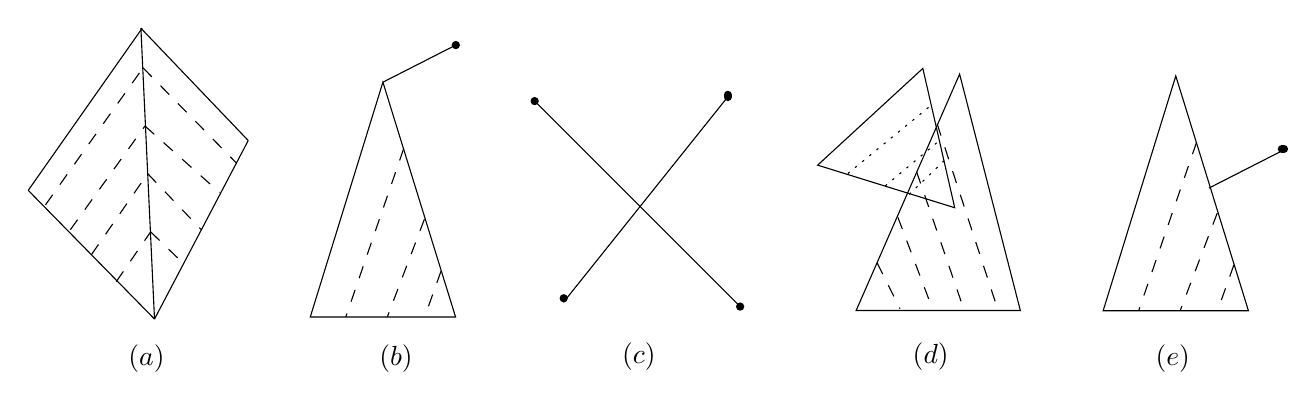
\begin{tikzpicture}[x=0.75pt,y=0.75pt,yscale=-1,xscale=1]
%uncomment if require: \path (0,300); %set diagram left start at 0, and has height of 300
%Straight Lines [id:da2433305781473396] 
\draw    (74.39,74) -- (126.11,128.11) ;
%Straight Lines [id:da6227399242346636] 
\draw    (75.01,74) -- (20.11,152.11) ;
%Straight Lines [id:da2605850731398158] 
\draw    (20.11,152.11) -- (80.95,214.11) ;
%Straight Lines [id:da8452031353987846] 
\draw    (80.95,214.11) -- (126.11,128.11) ;
%Straight Lines [id:da9893659492772733] 
\draw    (74.39,74) -- (80.95,214.11) ;
%Straight Lines [id:da5666990436403496] 
\draw  [dash pattern={on 4.5pt off 4.5pt}]  (28.41,159.11) -- (75.42,93.11) ;
%Straight Lines [id:da9463911730608483] 
\draw  [dash pattern={on 4.5pt off 4.5pt}]  (40.39,171.11) -- (76.34,121.11) ;
%Straight Lines [id:da3033443655778649] 
\draw  [dash pattern={on 4.5pt off 4.5pt}]  (50.53,183.11) -- (77.67,144.06) ;
%Straight Lines [id:da4740395971605613] 
\draw  [dash pattern={on 4.5pt off 4.5pt}]  (62.51,196.11) -- (79.1,172.11) ;
%Straight Lines [id:da45315048106015565] 
\draw  [dash pattern={on 4.5pt off 4.5pt}]  (79.1,172.11) -- (95.69,188.11) ;
%Straight Lines [id:da8142146081913095] 
\draw  [dash pattern={on 4.5pt off 4.5pt}]  (77.67,144.06) -- (103.53,171.11) ;
%Straight Lines [id:da8940757674809148] 
\draw  [dash pattern={on 4.5pt off 4.5pt}]  (76.34,121.11) -- (112.29,153.11) ;
%Straight Lines [id:da2573843730511203] 
\draw  [dash pattern={on 4.5pt off 4.5pt}]  (75.42,93.11) -- (120.58,139.11) ;
%Shape: Triangle [id:dp16571119505346799] 
\draw   (191,100) -- (226,213.11) -- (156,213.11) -- cycle ;
%Straight Lines [id:da1965612367742704] 
\draw  [dash pattern={on 4.5pt off 4.5pt}]  (201,132) -- (173.11,213.11) ;
%Straight Lines [id:da9312867516878975] 
\draw  [dash pattern={on 4.5pt off 4.5pt}]  (211,166) -- (193.11,213.11) ;
%Straight Lines [id:da9714161280437621] 
\draw  [dash pattern={on 4.5pt off 4.5pt}]  (219,191) -- (211.11,213.11) ;
%Straight Lines [id:da23084666962109224] 
\draw    (191,100) -- (226.11,82.11) ;
%Straight Lines [id:da7896712794084948] 
\draw    (264,109) -- (364,209) ;
%Straight Lines [id:da6414749028755078] 
\draw    (278,206) -- (357.11,107.11) ;
%Shape: Triangle [id:dp5612622822046731] 
\draw   (468.85,96.11) -- (498.11,210) -- (419,210) -- cycle ;
%Straight Lines [id:da19698622183489256] 
\draw  [dash pattern={on 4.5pt off 4.5pt}]  (429.11,187.11) -- (440.11,209.11) ;
%Straight Lines [id:da12675188454155584] 
\draw  [dash pattern={on 4.5pt off 4.5pt}]  (439.11,165.11) -- (456.11,210.11) ;
%Straight Lines [id:da011192874880048276] 
\draw  [dash pattern={on 4.5pt off 4.5pt}]  (448.11,143.11) -- (471.11,210.11) ;
%Straight Lines [id:da5270366769333337] 
\draw  [dash pattern={on 4.5pt off 4.5pt}]  (458,120) -- (487.11,209.11) ;
%Shape: Triangle [id:dp5770416539962782] 
\draw   (451.13,93.36) -- (466.49,160.48) -- (400.45,139.97) -- cycle ;
%Straight Lines [id:da05164565041458391] 
\draw  [dash pattern={on 0.84pt off 2.51pt}]  (444.56,154.06) -- (462.11,137.11) ;
%Straight Lines [id:da9411588517818319] 
\draw  [dash pattern={on 0.84pt off 2.51pt}]  (433,150) -- (459.11,128.11) ;
%Straight Lines [id:da5510688985707781] 
\draw  [dash pattern={on 0.84pt off 2.51pt}]  (415,144) -- (455.11,111.11) ;
%Shape: Triangle [id:dp07475980876949784] 
\draw   (573,97) -- (608,210.11) -- (538,210.11) -- cycle ;
%Straight Lines [id:da19702569241612622] 
\draw  [dash pattern={on 4.5pt off 4.5pt}]  (583,129) -- (555.11,210.11) ;
%Straight Lines [id:da7147258034299737] 
\draw  [dash pattern={on 4.5pt off 4.5pt}]  (593,163) -- (575.11,210.11) ;
%Straight Lines [id:da4878356421441634] 
\draw  [dash pattern={on 4.5pt off 4.5pt}]  (601,188) -- (593.11,210.11) ;
%Straight Lines [id:da05808148010059888] 
\draw    (589,151) -- (624.11,133.11) ;
%Shape: Free Drawing [id:dp9337003272798279] 
\draw  [line width=3] [line join = round][line cap = round] (278.11,204.11) .. controls (278.11,204.11) and (278.11,204.11) .. (278.11,204.11) ;
%Shape: Free Drawing [id:dp5934800956387472] 
\draw  [line width=3] [line join = round][line cap = round] (357.11,106.11) .. controls (357.11,106.44) and (357.11,106.78) .. (357.11,107.11) ;
%Shape: Free Drawing [id:dp9032497275218847] 
\draw  [line width=3] [line join = round][line cap = round] (363.11,208.11) .. controls (363.11,208.11) and (363.11,208.11) .. (363.11,208.11) ;
%Shape: Free Drawing [id:dp5037397828560217] 
\draw  [line width=3] [line join = round][line cap = round] (264.11,109.11) .. controls (264.11,109.11) and (264.11,109.11) .. (264.11,109.11) ;
%Shape: Free Drawing [id:dp547465563353533] 
\draw  [line width=3] [line join = round][line cap = round] (226.11,82.11) .. controls (226.11,82.11) and (226.11,82.11) .. (226.11,82.11) ;
%Shape: Free Drawing [id:dp8044607941509005] 
\draw  [line width=3] [line join = round][line cap = round] (624.11,132.11) .. controls (624.44,132.11) and (624.78,132.11) .. (625.11,132.11) ;

% Text Node
\draw (67.12,225.4) node [anchor=north west][inner sep=0.75pt]    {$( a)$};
% Text Node
\draw (188,225.4) node [anchor=north west][inner sep=0.75pt]    {$( b)$};
% Text Node
\draw (305,224.4) node [anchor=north west][inner sep=0.75pt]    {$( c)$};
% Text Node
\draw (445,224.4) node [anchor=north west][inner sep=0.75pt]    {$( d)$};
% Text Node
\draw (562,225.4) node [anchor=north west][inner sep=0.75pt]    {$( e)$};
\end{tikzpicture}\]
不难发现,上图中($a$)与($b$)是规则相处的,而($c$),($d$),($e$)则不是规则相处的.\\
但是,如果把($c$)中的图像看作四个单形拼起来的图形(在交点处增设一个顶点),那么它们是两两规则相处的.($d$),($e$)中的单形也可以进行类似处理,把它的2单形分成几个单形,使它们规则相处.
\begin{definition}
    设$K$是Euclid空间中有限个单形的集合,满足\\
    1) 若$[s]\in K$,则$[s]$的所有面都在$K$中\\
    2) $K$中任意两个单形规则相处,\\
    称这样的$K$是一个\emph{单纯复形},简称\emph{复形}.
\end{definition}

由定义,如果$[a_0,a_1,a_2]\in K$,则$[a_0],[a_1],[a_2],[a_0,a_1],[a_0,a_2],[a_1,a_2]$也都在复形$K$中(可以视为幂集为$K$的子集).\\
复形$K$的0单形叫做单纯复形的顶点,1单形叫做单纯复形的棱.复形$K$的维数是
$$
\text{dim } K = \left\{
    \begin{array}{c}
        -1, \text{当}K = \varnothing\\
        \max_{[s] \in K}\{\text{dim }[s]\}\\
    \end{array}
\right.
$$
其中$\text{dim }[s]$是单纯形$[s]$的维数.\\
如果复形$K$的子集$L$(也是一些单形的集合)本身也是一个复形,则称$L$为$K$的一个\emph{子复形}.\\
\begin{definition}
    设$K$为一个单纯复合型,赋予点集$\bigcup_{[s] \in K}[s]$Euclid空间的诱导拓扑锁构成的拓扑空间称为$K$决定的\emph{多面体},记作$|K|$,$\text{dim }K$也叫做多面体$K$的维数.如果$L$是$K$的子复形,称$(K,L)$为\emph{单纯复形偶},相应地,$(|K|,|L|)$叫做\emph{多面体偶}.
\end{definition}
也就是说,多面体$|K|$是由单纯复合形$K$的所有单纯形的点所成的点集.由单纯复合形的定义可知,多面体是由点,线段,三角形,四面体以及它们的高维类似物拼接起来的.\\
下面列举一些复形,多面体的简单性质,这些性质的证明都是容易的.
\begin{property}
    多面体是紧致的拓扑空间.
\end{property}
\begin{property}
    如果$L$是$K$的子复形,则$|L|$是$|K|$的闭子集.
\end{property}
\begin{property}
    多面体$|K|$是连通的当且仅当对于$K$中任意两个顶点$a$与$b$,存在$K$的一系列顶点$a = a_0,a_1,\cdots,a_r = b$使得$[a_0,a_1],[a_1,a_2],\cdots,[a_{r-1},a_r]$都是复形$K$的棱.
\end{property}
这样定义的多面体可以推广如下.
\begin{definition}
    设$X$是一个拓扑空间,如果存在复形$K$及其同胚映射$f : |K| \to X$,称$(K,f)$是空间$X$的一个\emph{单纯剖分},或\emph{三角剖分}.有时也简单地把$k$叫做$X$的一个单纯剖分,并把$X$称为一个\emph{可剖分空间}.
\end{definition}
\subsubsection{单纯复形的例子}
下面给出一些常用而又重要的例子,它们也同时给出了一些常见空间的单纯剖分.
\begin{example}
    设复形$K = \{[a_0],[a_1],[a_2],[a_0,a_1],[a_0,a_2],[a_1,a_2]\}$,它由三个顶点,三条棱组成,即$K$是一个由三角形的边缘组成的.显然$|K|$同胚于$S^1$,因此$K$可以看作是$S^1$的单纯剖分.\\
    不难看出$S^1$的单纯剖分并不唯一,但圆$S^1$在剖分以后至少有三个顶点.
    \[\tikzset{every picture/.style={line width=0.75pt}} %set default line width to 0.75pt        
    \begin{tikzpicture}[x=0.75pt,y=0.75pt,yscale=-1,xscale=1]
    %uncomment if require: \path (0,300); %set diagram left start at 0, and has height of 300
    
    %Shape: Triangle [id:dp7688697772661979] 
    \draw   (157.06,129) -- (214.11,226.33) -- (100,226.33) -- cycle ;
    %Curve Lines [id:da5868898957932644] 
    \draw    (247,181) .. controls (288.48,157.69) and (311.42,160.25) .. (345.44,180.08) ;
    \draw [shift={(347,181)}, rotate = 210.64] [color={rgb, 255:red, 0; green, 0; blue, 0 }  ][line width=0.75]    (10.93,-3.29) .. controls (6.95,-1.4) and (3.31,-0.3) .. (0,0) .. controls (3.31,0.3) and (6.95,1.4) .. (10.93,3.29)   ;
    %Shape: Circle [id:dp23627277424309012] 
    \draw   (375.5,177.56) .. controls (375.5,141.35) and (404.85,112) .. (441.06,112) .. controls (477.26,112) and (506.61,141.35) .. (506.61,177.56) .. controls (506.61,213.76) and (477.26,243.11) .. (441.06,243.11) .. controls (404.85,243.11) and (375.5,213.76) .. (375.5,177.56) -- cycle ;
    %Shape: Free Drawing [id:dp14651017333158234] 
    \draw  [line width=3] [line join = round][line cap = round] (393.11,132.33) .. controls (393.11,132.33) and (393.11,132.33) .. (393.11,132.33) ;
    %Shape: Free Drawing [id:dp9407187237683996] 
    \draw  [line width=3] [line join = round][line cap = round] (504.11,161.33) .. controls (504.11,161.33) and (504.11,161.33) .. (504.11,161.33) ;
    %Shape: Free Drawing [id:dp22203336219319914] 
    \draw  [line width=3] [line join = round][line cap = round] (421.11,240.33) .. controls (421.11,240.33) and (421.11,240.33) .. (421.11,240.33) ;
    
    % Text Node
    \draw (83,227.4) node [anchor=north west][inner sep=0.75pt]    {$a_{0}$};
    % Text Node
    \draw (216.11,229.73) node [anchor=north west][inner sep=0.75pt]    {$a_{1}$};
    % Text Node
    \draw (150,102.4) node [anchor=north west][inner sep=0.75pt]    {$a_{2}$};
    % Text Node
    \draw (295,141.4) node [anchor=north west][inner sep=0.75pt]    {$f$};
    % Text Node
    \draw (354,110.4) node [anchor=north west][inner sep=0.75pt]    {$f( a_{0})$};
    % Text Node
    \draw (389,253.4) node [anchor=north west][inner sep=0.75pt]    {$f( a_{1})$};
    % Text Node
    \draw (510,148.4) node [anchor=north west][inner sep=0.75pt]    {$f( a_{2})$};
    \end{tikzpicture}\]
\end{example}
\begin{example}
    下图左侧是一个Euclid空间$\mathbb{E}^3$中的一个三棱柱外侧(不包括顶部和底部)所成的图形,它有$6$个顶点,$12$条棱以及$6$个二维单形,它们组成一个复形$K$.右侧是复形$K$在平面上的一个示意图,此图中左右两侧的$[a_1,a_4]$在复形$K$中是同一条棱.
    \[\tikzset{every picture/.style={line width=0.75pt}} %set default line width to 0.75pt        
    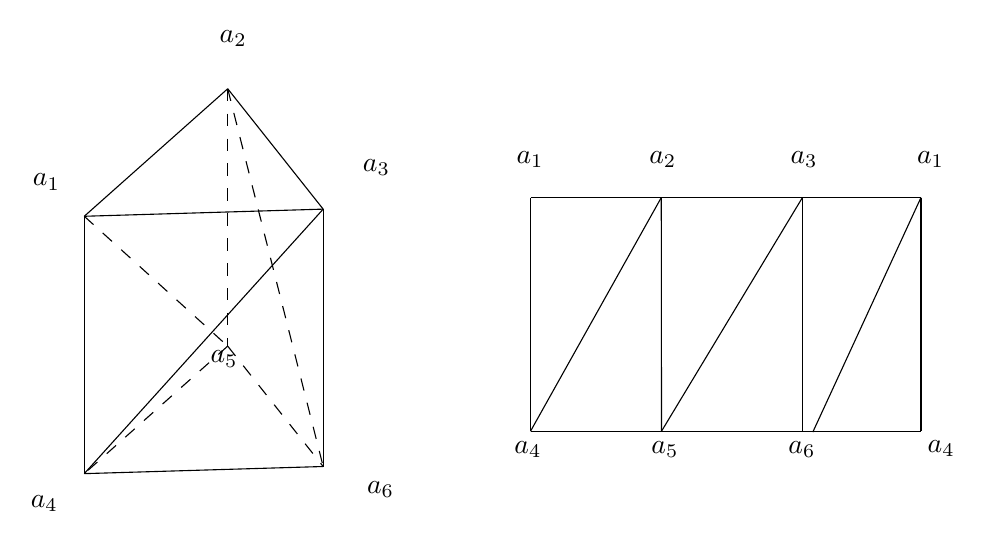
\begin{tikzpicture}[x=0.75pt,y=0.75pt,yscale=-1,xscale=1]
    %uncomment if require: \path (0,300); %set diagram left start at 0, and has height of 300
    
    %Straight Lines [id:da38488129770010215] 
    \draw    (177.11,56.56) -- (108,118) ;
    %Straight Lines [id:da4009196240846038] 
    \draw    (177.11,56.56) -- (223.11,114.56) ;
    %Straight Lines [id:da902225211129331] 
    \draw    (108,118) -- (223.11,114.56) ;
    %Straight Lines [id:da7435628323022323] 
    \draw    (108,118) -- (108,242) ;
    %Straight Lines [id:da9880503639939475] 
    \draw  [dash pattern={on 4.5pt off 4.5pt}]  (177.11,180.56) -- (108,242) ;
    %Straight Lines [id:da16527085136969855] 
    \draw  [dash pattern={on 4.5pt off 4.5pt}]  (177.11,180.56) -- (223.11,238.56) ;
    %Straight Lines [id:da8334881085338561] 
    \draw    (108,242) -- (223.11,238.56) ;
    %Straight Lines [id:da6833897637477797] 
    \draw  [dash pattern={on 4.5pt off 4.5pt}]  (177.11,56.56) -- (177.11,180.56) ;
    %Straight Lines [id:da14681862771817] 
    \draw    (223.11,114.56) -- (223.11,238.56) ;
    %Straight Lines [id:da6893512455245405] 
    \draw    (108,242) -- (223.11,114.56) ;
    %Straight Lines [id:da672621984482159] 
    \draw  [dash pattern={on 4.5pt off 4.5pt}]  (108,118) -- (177.11,180.56) ;
    %Straight Lines [id:da5790933795526962] 
    \draw  [dash pattern={on 4.5pt off 4.5pt}]  (177.11,56.56) -- (223.11,238.56) ;
    %Straight Lines [id:da9707450005595264] 
    \draw    (323,109) -- (511.11,109) ;
    %Straight Lines [id:da5245845660033037] 
    \draw    (323,109) -- (323,221.56) ;
    %Straight Lines [id:da27057055025138643] 
    \draw    (323,221.56) -- (511.11,221.56) ;
    %Straight Lines [id:da40203305768447706] 
    \draw    (511.11,109) -- (511.11,221.56) ;
    %Straight Lines [id:da6115939414929263] 
    \draw    (386,109) -- (386.11,221.56) ;
    %Straight Lines [id:da9801235769587859] 
    \draw    (454,109) -- (454,221.56) ;
    %Straight Lines [id:da47180768025426945] 
    \draw    (323,221.56) -- (386,109) ;
    %Straight Lines [id:da8006886386613494] 
    \draw    (386.11,221.56) -- (454,109) ;
    %Straight Lines [id:da7680416696298971] 
    \draw    (459,222) -- (511.11,109) ;
    
    % Text Node
    \draw (82,96.4) node [anchor=north west][inner sep=0.75pt]    {$a_{1}$};
    % Text Node
    \draw (172,27.4) node [anchor=north west][inner sep=0.75pt]    {$a_{2}$};
    % Text Node
    \draw (241,89.4) node [anchor=north west][inner sep=0.75pt]    {$a_{3}$};
    % Text Node
    \draw (81,251.4) node [anchor=north west][inner sep=0.75pt]    {$a_{4}$};
    % Text Node
    \draw (167.56,181.68) node [anchor=north west][inner sep=0.75pt]    {$a_{5}$};
    % Text Node
    \draw (243,244.4) node [anchor=north west][inner sep=0.75pt]    {$a_{6}$};
    % Text Node
    \draw (315,85.4) node [anchor=north west][inner sep=0.75pt]    {$a_{1}$};
    % Text Node
    \draw (379,85.4) node [anchor=north west][inner sep=0.75pt]    {$a_{2}$};
    % Text Node
    \draw (447,85.4) node [anchor=north west][inner sep=0.75pt]    {$a_{3}$};
    % Text Node
    \draw (508,85.4) node [anchor=north west][inner sep=0.75pt]    {$a_{1}$};
    % Text Node
    \draw (314,225.4) node [anchor=north west][inner sep=0.75pt]    {$a_{4}$};
    % Text Node
    \draw (380,225.4) node [anchor=north west][inner sep=0.75pt]    {$a_{5}$};
    % Text Node
    \draw (446,225.4) node [anchor=north west][inner sep=0.75pt]    {$a_{6}$};
    % Text Node
    \draw (513.11,224.96) node [anchor=north west][inner sep=0.75pt]    {$a_{4}$};
    
    
    \end{tikzpicture}\]
    不难发现,$|K|$同胚于柱面$S^1 \times I$,或平环$\{(x,y)\in\mathbb{E}^2:1\leq x^2+y^2 \leq 2\}$.因此上图中的复形$K$给出了下图柱面与平环的单纯剖分\\
\[\tikzset{every picture/.style={line width=0.75pt}} %set default line width to 0.75pt        
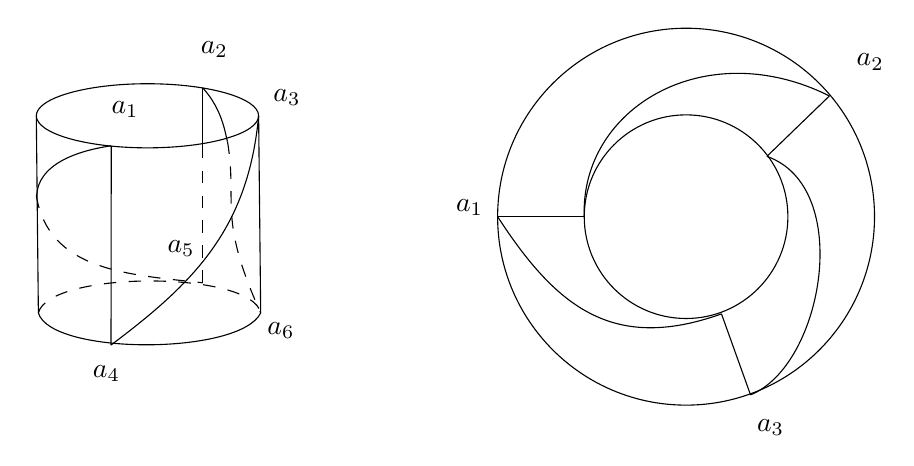
\begin{tikzpicture}[x=0.75pt,y=0.75pt,yscale=-1,xscale=1]
%uncomment if require: \path (0,300); %set diagram left start at 0, and has height of 300

%Shape: Circle [id:dp4999971914687651] 
\draw   (360,149.06) .. controls (360,121.96) and (381.96,100) .. (409.06,100) .. controls (436.15,100) and (458.11,121.96) .. (458.11,149.06) .. controls (458.11,176.15) and (436.15,198.11) .. (409.06,198.11) .. controls (381.96,198.11) and (360,176.15) .. (360,149.06) -- cycle ;
%Shape: Circle [id:dp33316983183423154] 
\draw   (318.26,149.06) .. controls (318.26,98.91) and (358.91,58.26) .. (409.06,58.26) .. controls (459.2,58.26) and (499.85,98.91) .. (499.85,149.06) .. controls (499.85,199.2) and (459.2,239.85) .. (409.06,239.85) .. controls (358.91,239.85) and (318.26,199.2) .. (318.26,149.06) -- cycle ;
%Straight Lines [id:da2690226183118438] 
\draw    (318.26,149.06) -- (360,149.06) ;
%Straight Lines [id:da6281857687908585] 
\draw    (448,120) -- (478.11,90.89) ;
%Straight Lines [id:da810061617294926] 
\draw    (426.11,195.89) -- (440.11,234.89) ;
%Curve Lines [id:da7015022745002477] 
\draw    (360,149.06) .. controls (358,96.89) and (418.11,60.89) .. (478.11,90.89) ;
%Curve Lines [id:da06919876782708978] 
\draw    (448,120) .. controls (490.11,134.89) and (475.11,220.89) .. (440.11,234.89) ;
%Curve Lines [id:da6035663429107088] 
\draw    (318.26,149.06) .. controls (346.11,191.89) and (373.22,214.78) .. (426.11,195.89) ;
%Shape: Ellipse [id:dp7359089288619383] 
\draw   (96,100.44) .. controls (96,91.91) and (119.98,85) .. (149.56,85) .. controls (179.13,85) and (203.11,91.91) .. (203.11,100.44) .. controls (203.11,108.97) and (179.13,115.89) .. (149.56,115.89) .. controls (119.98,115.89) and (96,108.97) .. (96,100.44) -- cycle ;
%Curve Lines [id:da20249362726404896] 
\draw    (97,195.44) .. controls (103.11,215.89) and (194.11,215.89) .. (204.11,195.44) ;
%Curve Lines [id:da3969475482249971] 
\draw  [dash pattern={on 4.5pt off 4.5pt}]  (97,195.44) .. controls (102.11,174.89) and (200.11,174.89) .. (204.11,195.44) ;
%Straight Lines [id:da24038990128553706] 
\draw    (96,100.44) -- (97,195.44) ;
%Straight Lines [id:da6295859681838718] 
\draw    (203.11,100.44) -- (204.11,195.44) ;
%Straight Lines [id:da4294706481322088] 
\draw    (132.11,114.89) -- (132,210.89) ;
%Straight Lines [id:da5457296850859954] 
\draw    (176.11,86.89) -- (176.11,114.89) ;
%Straight Lines [id:da13619207574101533] 
\draw  [dash pattern={on 4.5pt off 4.5pt}]  (176.11,114.89) -- (176.11,180.89) ;
%Curve Lines [id:da21393673179943629] 
\draw    (132.11,114.89) .. controls (92.11,120.89) and (97.11,139.89) .. (96,139) ;
%Curve Lines [id:da7856044799842534] 
\draw  [dash pattern={on 4.5pt off 4.5pt}]  (96,139) .. controls (102.11,174.89) and (139.11,176.89) .. (176.11,180.89) ;
%Curve Lines [id:da8144861182464729] 
\draw    (188.11,112.89) .. controls (187.11,109.89) and (186.11,97.89) .. (176.11,86.89) ;
%Curve Lines [id:da5354024775456783] 
\draw  [dash pattern={on 4.5pt off 4.5pt}]  (188.11,112.89) .. controls (193.11,142.89) and (183.11,148.89) .. (204.11,195.44) ;
%Curve Lines [id:da471795983694131] 
\draw    (132,210.89) .. controls (172,180.89) and (198.11,154.89) .. (203.11,100.44) ;

% Text Node
\draw (297,139.4) node [anchor=north west][inner sep=0.75pt]    {$a_{1}$};
% Text Node
\draw (490,69.4) node [anchor=north west][inner sep=0.75pt]    {$a_{2}$};
% Text Node
\draw (442,245.4) node [anchor=north west][inner sep=0.75pt]    {$a_{3}$};
% Text Node
\draw (131,92.4) node [anchor=north west][inner sep=0.75pt]    {$a_{1}$};
% Text Node
\draw (174,63.4) node [anchor=north west][inner sep=0.75pt]    {$a_{2}$};
% Text Node
\draw (209,86.4) node [anchor=north west][inner sep=0.75pt]    {$a_{3}$};
% Text Node
\draw (122,219.4) node [anchor=north west][inner sep=0.75pt]    {$a_{4}$};
% Text Node
\draw (158,159.4) node [anchor=north west][inner sep=0.75pt]    {$a_{5}$};
% Text Node
\draw (206.11,198.84) node [anchor=north west][inner sep=0.75pt]    {$a_{6}$};
\end{tikzpicture}\]
\end{example}
\begin{example}
    改变上例中左右两条棱的粘合方向(左)所得复形对应的拓扑空间为M\"{o}bius带(右,为展示其拼接,故与后文的彩色M\"{o}bius带不同).
    \[\tikzset{every picture/.style={line width=0.75pt}} %set default line width to 0.75pt        
    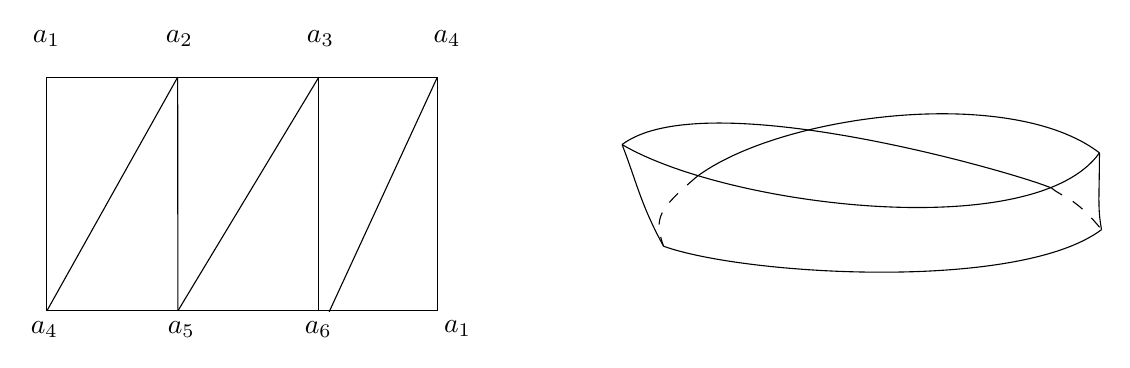
\begin{tikzpicture}[x=0.75pt,y=0.75pt,yscale=-1,xscale=1]
    %uncomment if require: \path (0,300); %set diagram left start at 0, and has height of 300
    
    %Straight Lines [id:da0055581689744395035] 
    \draw    (29,99) -- (217.11,99) ;
    %Straight Lines [id:da2712328604704062] 
    \draw    (29,99) -- (29,211.56) ;
    %Straight Lines [id:da9870370294330661] 
    \draw    (29,211.56) -- (217.11,211.56) ;
    %Straight Lines [id:da21130938076012007] 
    \draw    (217.11,99) -- (217.11,211.56) ;
    %Straight Lines [id:da042231172544964] 
    \draw    (92,99) -- (92.11,211.56) ;
    %Straight Lines [id:da24735570117875438] 
    \draw    (160,99) -- (160,211.56) ;
    %Straight Lines [id:da1550022448413797] 
    \draw    (29,211.56) -- (92,99) ;
    %Straight Lines [id:da7576857623847948] 
    \draw    (92.11,211.56) -- (160,99) ;
    %Straight Lines [id:da6415235113292541] 
    \draw    (165,212) -- (217.11,99) ;
    %Curve Lines [id:da09173392017805604] 
    \draw    (342,147) .. controls (382,117) and (493.11,102.44) .. (536.11,135.44) ;
    %Curve Lines [id:da9058908298243264] 
    \draw    (306.11,131.44) .. controls (346.11,101.44) and (497.11,145.44) .. (513.11,152.44) ;
    %Curve Lines [id:da9483158334746751] 
    \draw    (306.11,131.44) .. controls (313.11,149.44) and (315.11,160.44) .. (326.11,180.44) ;
    %Curve Lines [id:da29804912384137805] 
    \draw    (326.11,180.44) .. controls (365.11,194.44) and (497.11,202.44) .. (537.11,172.44) ;
    %Curve Lines [id:da9038345629182629] 
    \draw    (306.11,131.44) .. controls (357.11,161.44) and (505.11,179.44) .. (536.11,135.44) ;
    %Curve Lines [id:da8113728658567991] 
    \draw    (536.11,135.44) .. controls (536.11,156.44) and (535.11,161.44) .. (537.11,172.44) ;
    %Curve Lines [id:da7161756904337369] 
    \draw  [dash pattern={on 4.5pt off 4.5pt}]  (513.11,152.44) .. controls (519.11,157.44) and (524.11,156.44) .. (537.11,172.44) ;
    %Curve Lines [id:da9023307000598448] 
    \draw  [dash pattern={on 4.5pt off 4.5pt}]  (342,147) .. controls (324.11,162.44) and (321.11,166.44) .. (326.11,180.44) ;
    
    % Text Node
    \draw (21,75.4) node [anchor=north west][inner sep=0.75pt]    {$a_{1}$};
    % Text Node
    \draw (85,75.4) node [anchor=north west][inner sep=0.75pt]    {$a_{2}$};
    % Text Node
    \draw (153,75.4) node [anchor=north west][inner sep=0.75pt]    {$a_{3}$};
    % Text Node
    \draw (214,75.4) node [anchor=north west][inner sep=0.75pt]    {$a_{4}$};
    % Text Node
    \draw (20,215.4) node [anchor=north west][inner sep=0.75pt]    {$a_{4}$};
    % Text Node
    \draw (86,215.4) node [anchor=north west][inner sep=0.75pt]    {$a_{5}$};
    % Text Node
    \draw (152,215.4) node [anchor=north west][inner sep=0.75pt]    {$a_{6}$};
    % Text Node
    \draw (219.11,214.96) node [anchor=north west][inner sep=0.75pt]    {$a_{1}$};
    
    
    \end{tikzpicture}\]      
\end{example}
\begin{example}
    环面$T^2$的单纯剖分.\\
    将环面沿一个经圆剪开,得到的图形同胚于圆柱面,再把圆柱面沿一半剪开,得到一个长方形,因此环面可以视为一个长方形的对边粘合二乘,下图的左侧是环面的一个单纯剖分示意图
    \[\tikzset{every picture/.style={line width=0.75pt}} %set default line width to 0.75pt        
    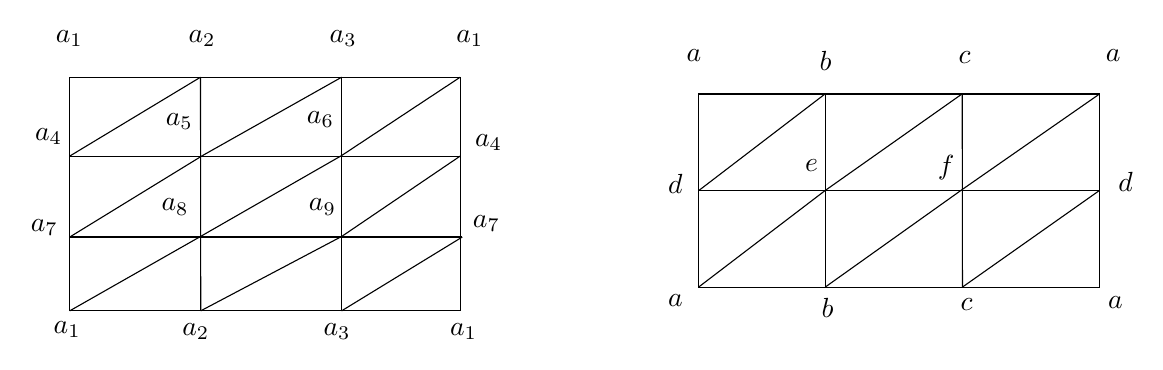
\begin{tikzpicture}[x=0.75pt,y=0.75pt,yscale=-1,xscale=1]
    %uncomment if require: \path (0,300); %set diagram left start at 0, and has height of 300
    
    %Straight Lines [id:da7989479221499458] 
    \draw    (51,119) -- (239.11,119) ;
    %Straight Lines [id:da8996601749247204] 
    \draw    (51,119) -- (51,231.56) ;
    %Straight Lines [id:da3769336094434623] 
    \draw    (51,231.56) -- (239.11,231.56) ;
    %Straight Lines [id:da033941692961417136] 
    \draw    (239.11,119) -- (239.11,231.56) ;
    %Straight Lines [id:da028273873005895123] 
    \draw    (114,119) -- (114.11,231.56) ;
    %Straight Lines [id:da7338319664431581] 
    \draw    (182,119) -- (182,231.56) ;
    %Straight Lines [id:da8625916947156347] 
    \draw    (51,157) -- (239.11,157) ;
    %Straight Lines [id:da09701707716036245] 
    \draw    (51,196) -- (240.11,196) ;
    %Straight Lines [id:da08471352802410026] 
    \draw    (51,157) -- (114,119) ;
    %Straight Lines [id:da09889876483958271] 
    \draw    (51,196) -- (115.11,156.67) ;
    %Straight Lines [id:da7288846292407272] 
    \draw    (115.11,156.67) -- (182,119) ;
    %Straight Lines [id:da7611493801007239] 
    \draw    (51,231.56) -- (114.11,195.67) ;
    %Straight Lines [id:da5149795584463694] 
    \draw    (114.11,195.67) -- (182.11,156.67) ;
    %Straight Lines [id:da634888860170189] 
    \draw    (182.11,156.67) -- (239.11,119) ;
    %Straight Lines [id:da19006411075543417] 
    \draw    (114.11,231.56) -- (182.11,195.67) ;
    %Straight Lines [id:da7867428813984834] 
    \draw    (182.11,195.67) -- (239.11,157) ;
    %Straight Lines [id:da8756835281385549] 
    \draw    (182,231.56) -- (240.11,196) ;
    %Shape: Rectangle [id:dp1057184375808553] 
    \draw   (354,127.11) -- (547.11,127.11) -- (547.11,220.11) -- (354,220.11) -- cycle ;
    %Straight Lines [id:da9212941839836413] 
    \draw    (354.06,173.61) -- (547.06,173.61) ;
    %Straight Lines [id:da0846579165502479] 
    \draw    (415,127) -- (415,220.11) ;
    %Straight Lines [id:da6648297712008773] 
    \draw    (481,127) -- (481.11,220.11) ;
    %Straight Lines [id:da4753162849411614] 
    \draw    (354,220.11) -- (415,173.56) ;
    %Straight Lines [id:da6545720407055529] 
    \draw    (354.06,173.61) -- (415,127) ;
    %Straight Lines [id:da030190303537098284] 
    \draw    (415,173.56) -- (481,127) ;
    %Straight Lines [id:da2045170510463299] 
    \draw    (415,220.11) -- (481.06,173.06) ;
    %Straight Lines [id:da13118660478310784] 
    \draw    (481.06,173.06) -- (547.11,127.11) ;
    %Straight Lines [id:da7952153838369707] 
    \draw    (481.11,220.11) -- (547.06,173.61) ;
    
    % Text Node
    \draw (43,95.4) node [anchor=north west][inner sep=0.75pt]    {$a_{1}$};
    % Text Node
    \draw (107,95.4) node [anchor=north west][inner sep=0.75pt]    {$a_{2}$};
    % Text Node
    \draw (175,95.4) node [anchor=north west][inner sep=0.75pt]    {$a_{3}$};
    % Text Node
    \draw (236,95.4) node [anchor=north west][inner sep=0.75pt]    {$a_{1}$};
    % Text Node
    \draw (42,235.4) node [anchor=north west][inner sep=0.75pt]    {$a_{1}$};
    % Text Node
    \draw (33,142.4) node [anchor=north west][inner sep=0.75pt]    {$a_{4}$};
    % Text Node
    \draw (96,135.4) node [anchor=north west][inner sep=0.75pt]    {$a_{5}$};
    % Text Node
    \draw (164,134.4) node [anchor=north west][inner sep=0.75pt]    {$a_{6}$};
    % Text Node
    \draw (245,145.4) node [anchor=north west][inner sep=0.75pt]    {$a_{4}$};
    % Text Node
    \draw (31,186.4) node [anchor=north west][inner sep=0.75pt]    {$a_{7}$};
    % Text Node
    \draw (94,176.4) node [anchor=north west][inner sep=0.75pt]    {$a_{8}$};
    % Text Node
    \draw (104,236.4) node [anchor=north west][inner sep=0.75pt]    {$a_{2}$};
    % Text Node
    \draw (172,236.4) node [anchor=north west][inner sep=0.75pt]    {$a_{3}$};
    % Text Node
    \draw (233,236.4) node [anchor=north west][inner sep=0.75pt]    {$a_{1}$};
    % Text Node
    \draw (165,176.4) node [anchor=north west][inner sep=0.75pt]    {$a_{9}$};
    % Text Node
    \draw (244,184.4) node [anchor=north west][inner sep=0.75pt]    {$a_{7}$};
    % Text Node
    \draw (347,104.4) node [anchor=north west][inner sep=0.75pt]    {$a$};
    % Text Node
    \draw (411,105.4) node [anchor=north west][inner sep=0.75pt]    {$b$};
    % Text Node
    \draw (478,105.4) node [anchor=north west][inner sep=0.75pt]    {$c$};
    % Text Node
    \draw (338,164.4) node [anchor=north west][inner sep=0.75pt]    {$d$};
    % Text Node
    \draw (549,104.4) node [anchor=north west][inner sep=0.75pt]    {$a$};
    % Text Node
    \draw (404,157.4) node [anchor=north west][inner sep=0.75pt]    {$e$};
    % Text Node
    \draw (468,155.4) node [anchor=north west][inner sep=0.75pt]    {$f$};
    % Text Node
    \draw (555,163.4) node [anchor=north west][inner sep=0.75pt]    {$d$};
    % Text Node
    \draw (338,222.4) node [anchor=north west][inner sep=0.75pt]    {$a$};
    % Text Node
    \draw (412,224.4) node [anchor=north west][inner sep=0.75pt]    {$b$};
    % Text Node
    \draw (479,224.4) node [anchor=north west][inner sep=0.75pt]    {$c$};
    % Text Node
    \draw (550,223.4) node [anchor=north west][inner sep=0.75pt]    {$a$};
    
    
    \end{tikzpicture}\]
    上图左侧就是一个环面的单纯剖分的平面示意图,它共有$9$个顶点,$27$条棱,$18$个三角形.\\
    但是上图右侧的图形并不能表示环面的单纯剖分.此图中连接点$e,b$的两条线段,这两条线段在环面上是不同的.但是在对应的复形中只能有一个1单形,也就是说,如果此图表示一个复形,那么在对应的多面体中以$e,b$为端点的两条线段应叠合称一条.同样,三点$e,f,b$在下半图形构成一个2单形,而在上半图形三点$e,f,b$不构成单形.因此右边的图形不能表示任何一个复形,自然也不是环面的单纯剖分.在叠合长方形得到环面$T^2$时,只能沿两边叠合,而不能把内部点也叠合.
\end{example}
\begin{example}
    Klein瓶的单纯剖分.\\
    把上图中的左图改为下图左侧形式,所得到的空间就是Klein瓶,它是将一个长方形的一对对边按照上例的方法叠合后,将令一对对边按照反方向叠合得到的.
    \[\tikzset{every picture/.style={line width=0.75pt}} %set default line width to 0.75pt        
    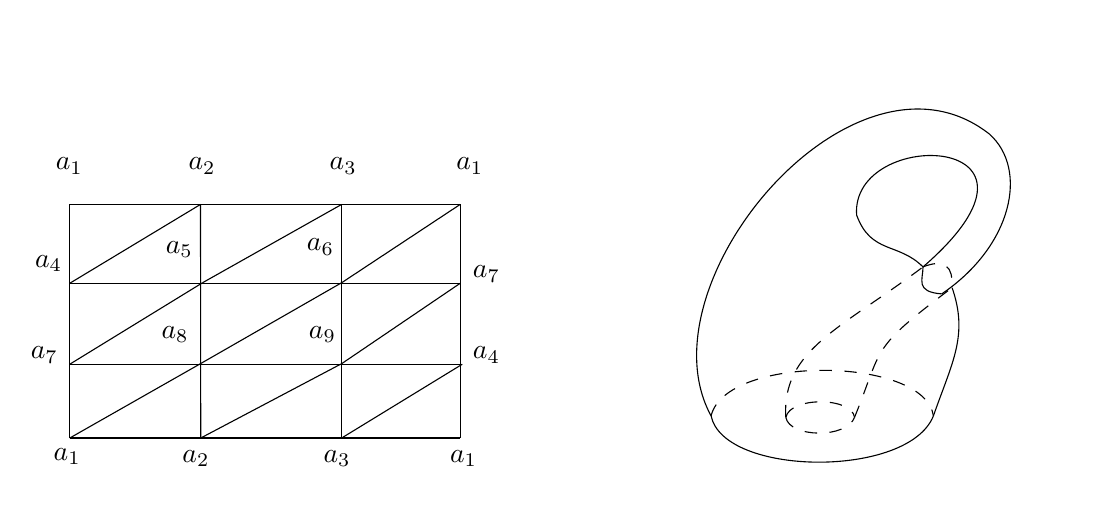
\begin{tikzpicture}[x=0.75pt,y=0.75pt,yscale=-1,xscale=1]
    %uncomment if require: \path (0,300); %set diagram left start at 0, and has height of 300
    
    %Straight Lines [id:da506679835350013] 
    \draw    (71,134.56) -- (259.11,134.56) ;
    %Straight Lines [id:da4845047158832321] 
    \draw    (71,134.56) -- (71,247.11) ;
    %Straight Lines [id:da8910182833878773] 
    \draw    (71,247.11) -- (259.11,247.11) ;
    %Straight Lines [id:da007708263540063154] 
    \draw    (259.11,134.56) -- (259.11,247.11) ;
    %Straight Lines [id:da8720985924033293] 
    \draw    (134,134.56) -- (134.11,247.11) ;
    %Straight Lines [id:da7113577614710846] 
    \draw    (202,134.56) -- (202,247.11) ;
    %Straight Lines [id:da9875000219738654] 
    \draw    (71,172.56) -- (259.11,172.56) ;
    %Straight Lines [id:da9212902342238742] 
    \draw    (71,211.56) -- (260.11,211.56) ;
    %Straight Lines [id:da43872921507480855] 
    \draw    (71,172.56) -- (134,134.56) ;
    %Straight Lines [id:da6497612287633825] 
    \draw    (71,211.56) -- (135.11,172.22) ;
    %Straight Lines [id:da4536181251286624] 
    \draw    (135.11,172.22) -- (202,134.56) ;
    %Straight Lines [id:da5009602691426858] 
    \draw    (71,247.11) -- (134.11,211.22) ;
    %Straight Lines [id:da23743114286944222] 
    \draw    (134.11,211.22) -- (202.11,172.22) ;
    %Straight Lines [id:da8540150403682925] 
    \draw    (202.11,172.22) -- (259.11,134.56) ;
    %Straight Lines [id:da4434289447600537] 
    \draw    (134.11,247.11) -- (202.11,211.22) ;
    %Straight Lines [id:da7072433373714824] 
    \draw    (202.11,211.22) -- (259.11,172.56) ;
    %Straight Lines [id:da7634830512009461] 
    \draw    (202,247.11) -- (260.11,211.56) ;
    %Curve Lines [id:da7737090620797373] 
    \draw    (380,236.44) .. controls (386.11,265.67) and (475.11,266.67) .. (487.11,236.44) ;
    %Curve Lines [id:da4320938959669849] 
    \draw  [dash pattern={on 4.5pt off 4.5pt}]  (380,236.44) .. controls (387.11,206.67) and (483.11,207.67) .. (487.11,236.44) ;
    %Curve Lines [id:da537722731775327] 
    \draw    (380,236.44) .. controls (345.11,172.67) and (449.11,49.67) .. (514.11,100.67) ;
    %Curve Lines [id:da40122973886210245] 
    \draw    (491.11,177.67) .. controls (525.11,154.67) and (533.11,117.67) .. (514.11,100.67) ;
    %Curve Lines [id:da1398572087447989] 
    \draw    (450.11,139.67) .. controls (447.11,96.67) and (557.11,99.67) .. (482.11,164.67) ;
    %Curve Lines [id:da427916102297456] 
    \draw    (450.11,139.67) .. controls (457.11,158.67) and (470.11,152.67) .. (482.11,164.67) ;
    %Curve Lines [id:da5138195479726921] 
    \draw    (487.11,236.44) .. controls (496.11,210.67) and (504.11,197.67) .. (496.11,174.67) ;
    %Curve Lines [id:da44855680334007664] 
    \draw    (482.11,164.67) .. controls (482.11,170.67) and (478.11,176.67) .. (491.11,177.67) ;
    %Curve Lines [id:da639703168923053] 
    \draw  [dash pattern={on 4.5pt off 4.5pt}]  (482.11,164.67) .. controls (497.11,158.67) and (496.11,170.67) .. (496.11,174.67) ;
    %Curve Lines [id:da18765334443769133] 
    \draw  [dash pattern={on 4.5pt off 4.5pt}]  (416,237.15) .. controls (417.89,247.1) and (445.4,247.44) .. (449.11,237.15) ;
    %Curve Lines [id:da26792373501200273] 
    \draw  [dash pattern={on 4.5pt off 4.5pt}]  (416,237.15) .. controls (418.2,227) and (447.87,227.34) .. (449.11,237.15) ;
    %Curve Lines [id:da3740479845293898] 
    \draw  [dash pattern={on 4.5pt off 4.5pt}]  (416,237.15) .. controls (414.11,204.67) and (442.11,194.67) .. (482.11,164.67) ;
    %Curve Lines [id:da9749798365296474] 
    \draw  [dash pattern={on 4.5pt off 4.5pt}]  (449.11,237.15) .. controls (463.11,202.67) and (456.11,204.67) .. (496.11,174.67) ;
    
    % Text Node
    \draw (63,110.96) node [anchor=north west][inner sep=0.75pt]    {$a_{1}$};
    % Text Node
    \draw (127,110.96) node [anchor=north west][inner sep=0.75pt]    {$a_{2}$};
    % Text Node
    \draw (195,110.96) node [anchor=north west][inner sep=0.75pt]    {$a_{3}$};
    % Text Node
    \draw (256,110.96) node [anchor=north west][inner sep=0.75pt]    {$a_{1}$};
    % Text Node
    \draw (62,250.96) node [anchor=north west][inner sep=0.75pt]    {$a_{1}$};
    % Text Node
    \draw (53,157.96) node [anchor=north west][inner sep=0.75pt]    {$a_{4}$};
    % Text Node
    \draw (116,150.96) node [anchor=north west][inner sep=0.75pt]    {$a_{5}$};
    % Text Node
    \draw (184,149.96) node [anchor=north west][inner sep=0.75pt]    {$a_{6}$};
    % Text Node
    \draw (264,201.96) node [anchor=north west][inner sep=0.75pt]    {$a_{4}$};
    % Text Node
    \draw (51,201.96) node [anchor=north west][inner sep=0.75pt]    {$a_{7}$};
    % Text Node
    \draw (114,191.96) node [anchor=north west][inner sep=0.75pt]    {$a_{8}$};
    % Text Node
    \draw (124,251.96) node [anchor=north west][inner sep=0.75pt]    {$a_{2}$};
    % Text Node
    \draw (192,251.96) node [anchor=north west][inner sep=0.75pt]    {$a_{3}$};
    % Text Node
    \draw (253,251.96) node [anchor=north west][inner sep=0.75pt]    {$a_{1}$};
    % Text Node
    \draw (185,191.96) node [anchor=north west][inner sep=0.75pt]    {$a_{9}$};
    % Text Node
    \draw (264,162.96) node [anchor=north west][inner sep=0.75pt]    {$a_{7}$};
    \end{tikzpicture}\]
\end{example}
\begin{example}
    射影空间$\mathbb{R}P^2$的单纯剖分.\\
    射影空间$\mathbb{R}P^2$是将球面$S^2$的每一对对称点叠合而成,它也可以看成是将单位圆盘$D^2$的边界$S^1$上对称点的叠合,而内部点保持不变得到,它的一个三角剖分如下图所示
    \[\tikzset{every picture/.style={line width=0.75pt}} %set default line width to 0.75pt        
    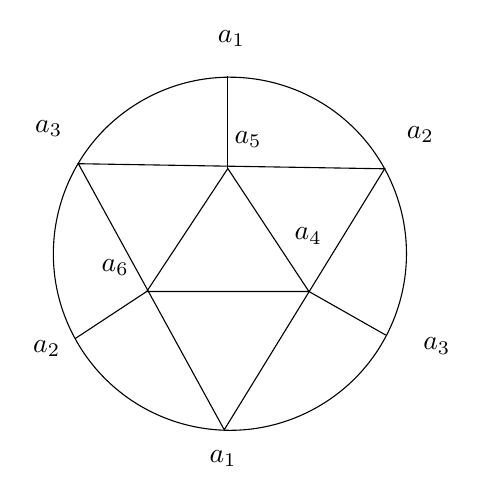
\begin{tikzpicture}[x=0.75pt,y=0.75pt,yscale=-1,xscale=1]
    %uncomment if require: \path (0,300); %set diagram left start at 0, and has height of 300
    
    %Shape: Circle [id:dp5849839847158507] 
    \draw   (153.16,70.48) .. controls (194.35,47.89) and (246.05,62.97) .. (268.63,104.16) .. controls (291.22,145.35) and (276.14,197.05) .. (234.95,219.63) .. controls (193.77,242.22) and (142.07,227.14) .. (119.48,185.95) .. controls (96.89,144.77) and (111.97,93.07) .. (153.16,70.48) -- cycle ;
    %Shape: Triangle [id:dp5152748146574699] 
    \draw   (268.61,104.12) -- (191.33,229.87) -- (121.03,101.67) -- cycle ;
    %Shape: Triangle [id:dp4782679961597993] 
    \draw   (193.06,104) -- (232.11,163.22) -- (154,163.22) -- cycle ;
    %Straight Lines [id:da5398997059934596] 
    \draw    (193.06,59.22) -- (193.06,104) ;
    %Straight Lines [id:da30367944665267776] 
    \draw    (154,163.22) -- (119.48,185.95) ;
    %Straight Lines [id:da9086924350885073] 
    \draw    (232.11,163.22) -- (269.11,184.22) ;
    
    % Text Node
    \draw (187,36.4) node [anchor=north west][inner sep=0.75pt]    {$a_{1}$};
    % Text Node
    \draw (183,238.4) node [anchor=north west][inner sep=0.75pt]    {$a_{1}$};
    % Text Node
    \draw (98,185.4) node [anchor=north west][inner sep=0.75pt]    {$a_{2}$};
    % Text Node
    \draw (278,82.4) node [anchor=north west][inner sep=0.75pt]    {$a_{2}$};
    % Text Node
    \draw (286,184.4) node [anchor=north west][inner sep=0.75pt]    {$a_{3}$};
    % Text Node
    \draw (99,79.4) node [anchor=north west][inner sep=0.75pt]    {$a_{3}$};
    % Text Node
    \draw (224,131.4) node [anchor=north west][inner sep=0.75pt]    {$a_{4}$};
    % Text Node
    \draw (195.06,85.01) node [anchor=north west][inner sep=0.75pt]    {$a_{5}$};
    % Text Node
    \draw (131,146.4) node [anchor=north west][inner sep=0.75pt]    {$a_{6}$};
    \end{tikzpicture}\]
\end{example}
\begin{example}
    球面$S^n$的单纯剖分.\\
    设$[a_0,a_1,\cdots,a_{n+1}]$是一个$n+1$维单形,它的所有维数小于$n+1$的面构成一个复形$K$,易见$|K| \cong S^n$.
\end{example}
\subsubsection{单形的定向}
设$K = \{[s_i^q]: i = 1,2,\cdots,a_q;q = 0,1,\cdots,n\}$是一个$n$维复形,$[s_1^q],\cdots,[s^q_{\alpha_q}]$是它的$\alpha_q$个$q$维单形.
\begin{definition}
    对一个单形的顶点给定一个排列,叫做给出了该单形的一个\emph{定向}.如果两个排列差了一个偶置换,称给出的定向相同;如果相差一个奇置换,给出的定向相反.指定了定向的单形叫做\emph{定向单形}.
\end{definition}
例如,单形$[s] = [a,b,c]$的顶点不同排列有
$$
abc,bca,cab,acb,cba,bac
$$
其中前三个与后三个给出的定向分别相同,而这两组排列给出的定向不同.我们用下式表示这些定向的关系.
$$
abc = bca = cab  = -acb = -cba = -bac
$$
也就是说,我们用等号表示相同定向的排列,而用$-$表示定向相反的排列.\\
由定义,每个单形有两个定向.设$[s] = [a_0,a_1,\cdots,a_q]$是一个$q$单形,$a_0a_1a_2\cdots a_q$与$a_1a_0a_2\cdots a_q$给出了$[s]$的两个定向,$[s]$的顶点的其他排列给出的定向分别可以这两个排列来表示.$a_0a_1a_2\cdots a_q$与$a_1a_0a_2\cdots a_q$等都叫做定向单形.0单形$[a_0]$也有两个定向,分别记为$a_0$与$-a_0$.\\
此后,对于$q$维单形,我们一般记其为$\Delta_q$
\newpage
\section{同伦}
\subsection{预备知识}
对于任何两个拓扑空间$X,Y$,记
$$
Y^X := \text{Hom}(X,Y)
$$
在$Y^X$中可以赋予一个紧开拓扑使其成为一个拓扑空间.


那么,紧开拓扑又是何方神圣呢?
\begin{definition}
    记$T = \{X\text{中所有紧致子集}\}$,$F = \{Y\text{中所有的开集}\}$.对于所有的$K \in T$以及$Y \in U$,记$N(K,U) = \{f: X \to Y : f(K)\subset U\}$.则
    $$
    \mathscr{B} = \{N(K,U) : K \in T, U \in F\}
    $$
    是$Y^X$的一个拓扑基,它可以生成$Y^X$的一个拓扑,称为$Y^X$的一个紧开拓扑
    \label{Def:1.1.1}
\end{definition}

接下来我们验证定义\ref{Def:1.1.1}中$\mathscr{B}$确实是$Y^X$的一个拓扑基.


根据我们在点集拓扑的知识可以得到引理\ref{Lem:1.1.1}
\begin{lemma}
$X$的子集族$\mathscr{B}$能够成为$X$上某个拓扑的基的充要条件为:


1. $X= \bigcup_{B \in \mathscr{B}} B$;


2. 对任意$B_1,B_2 \in \mathscr{B}$,交集$B_1\cap B_2$可以表示为$\mathscr{B}$中某些成员的并集
\label{Lem:1.1.1}
\end{lemma}
\begin{proof}


必要性:


设$\mathscr{B}$为某个拓扑$\mathscr{T}$的基.


因为$X$是开集,1. 显然满足.


因为$\mathscr{B}$中的成员均为开集.因此对于任意的$B_1,B_2 \in \mathscr{B}$都有$B_1 \cap B_2$是开集.根据基的定义可知2.自然满足.


充分性:


设$\mathscr{B}$为满足条件的子集族.作$\mathscr{B}$中所有可能的并集,记其全体为$\mathscr{T}$.不难发现$\mathscr{T}$满足$\bigcup \mathscr{T} = X$且$\varnothing \in \mathscr{T}$.且$\mathscr{T}$的任意并均属于$\mathscr{T}$(即也为开集).


而后设$U_1,U_2 \in \mathscr{T}$.当$U_1 \cap U_2 = \varnothing$时显然有$U_1 \cap U_2 \in \mathscr{T}$.当$U_1 \cap U_2 \neq \varnothing$时,由于$\mathscr{T}$为$\mathscr{B}$中所有可能并集的全体,因此可以得到对于任意的$x \in U_1 \cap U_2$存在$B_1,B_2$使得$x \in B_1$且$x \in B_2$.从而有$x \in B_1 \cap B_2 \subset U_1 \cap U_2$.根据2.可以知道存在$B_x\in \mathscr{B}$使得$x\in B_x \subset B_1 \cap B_2 \subset U_1 \cap U_2$.因此有$U_1 \cap U_2 = \bigcup_{x \in U_1 \cap U_2}B_x \in \mathscr{T}$
\end{proof}
因此我们只需要验证定义\ref{Def:1.1.1}的$\mathscr{B}$满足引理\ref{Lem:1.1.1}的条件即可.
\begin{proof}
    (定义\ref{Def:1.1.1}验证)


    1. 考虑$\bigcup_{K,U}N(K,U)$,不难发现对于任意的$f \in Y^X$,考虑$K \in T$由于$K$为紧集,因此$f(K)$也是一个紧集,因此对于$f(K)$总是存在一个开覆盖$U$使得$f(K) \subset U$,而由于开集的任意并集也是开集,因此$\bigcup U \in F$.因此有$f \in \bigcup_{K,U}N(K,U)$即$Y^X \subset \bigcup_{K,U}N(K,U)$至于反向的包含是显然的.因此1.满足


    2. 考虑$N(K,U)$与$N(K',U')$的交集,即$N(K,U) \cap N(K',U')$其表示所有的同时满足$f(K) \subset U$和$f(K') \subset U'$由于紧集的定义为所有的开覆盖均有有限子覆盖,因此考虑任意的$K \cup K'$的开覆盖,不难发现其也具有一个有限子覆盖,即它也是一个紧集,因此$N(K,U) \cap N(K',U') = N(K \cup K',U \cup U')$
    因此2.满足


    使用引理\ref{Lem:1.1.1}可以直接得到$\mathscr{B}$确实是一个拓扑基
\end{proof}


一般将赋予了紧开拓扑的拓扑空间$(Y^X,\mathscr{T})$称为映射空间.


但是在代数拓扑中,我们一般不会用到映射空间的概念,一般只将$Y^X$当作一个集合来使用.
 

\subsection{同伦与拓扑空间的同伦型}
\subsubsection{基本概念}
在讲同伦之前,我们先使用一个例子来说明同伦是什么.
\begin{example}
记$X = \{(x,y) \in \mathbb{R}^2: 1 \leq x^2+y^2 <2\}$,$S^1$为一个Euclid空间中的标准圆

由于$X$不是有界闭集,因此$X$在Euclid空间中不是紧致的,而$S^1$是紧致的,因此两者必然不会同胚.
而我们现在打算构建一个从$X$到$S^1$随着时间进行连续变化的映射$F : X\times I \to X$,其中$I$为一个单位的闭区间$[0,1]$使得对于$t\in I$,$t = 0$时$F(x,0) = x$,而$t = 1$时$F(x,1) \in S^1$,并且还有$f(X,1) = S^1$.


其具体的变化方式就如下图所示:
\[\tikzset{every picture/.style={line width=0.75pt}} %set default line width to 0.75pt       
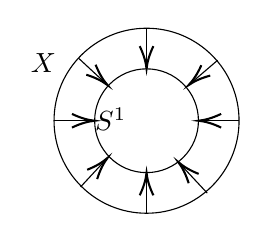
\begin{tikzpicture}[x=0.75pt,y=0.75pt,yscale=-1,xscale=1]
%uncomment if require: \path (0,223); %set diagram left start at 0, and has height of 223

%Shape: Circle [id:dp4925840575678846] 
\draw   (326,107) .. controls (326,93.19) and (337.19,82) .. (351,82) .. controls (364.81,82) and (376,93.19) .. (376,107) .. controls (376,120.81) and (364.81,132) .. (351,132) .. controls (337.19,132) and (326,120.81) .. (326,107) -- cycle ;
%Shape: Circle [id:dp6673585714851444] 
\draw   (306.43,107) .. controls (306.43,82.38) and (326.38,62.43) .. (351,62.43) .. controls (375.62,62.43) and (395.57,82.38) .. (395.57,107) .. controls (395.57,131.62) and (375.62,151.57) .. (351,151.57) .. controls (326.38,151.57) and (306.43,131.62) .. (306.43,107) -- cycle ;
%Straight Lines [id:da05623028261190144] 
\draw    (306.43,107) -- (324,107) ;
\draw [shift={(326,107)}, rotate = 180] [color={rgb, 255:red, 0; green, 0; blue, 0 }  ][line width=0.75]    (10.93,-3.29) .. controls (6.95,-1.4) and (3.31,-0.3) .. (0,0) .. controls (3.31,0.3) and (6.95,1.4) .. (10.93,3.29)   ;
%Straight Lines [id:da6061966896035791] 
\draw    (351,62.43) -- (351,80) ;
\draw [shift={(351,82)}, rotate = 270] [color={rgb, 255:red, 0; green, 0; blue, 0 }  ][line width=0.75]    (10.93,-3.29) .. controls (6.95,-1.4) and (3.31,-0.3) .. (0,0) .. controls (3.31,0.3) and (6.95,1.4) .. (10.93,3.29)   ;
%Straight Lines [id:da8942552451634078] 
\draw    (318.24,76.86) -- (330.77,88.5) ;
\draw [shift={(332.24,89.86)}, rotate = 222.88] [color={rgb, 255:red, 0; green, 0; blue, 0 }  ][line width=0.75]    (10.93,-3.29) .. controls (6.95,-1.4) and (3.31,-0.3) .. (0,0) .. controls (3.31,0.3) and (6.95,1.4) .. (10.93,3.29)   ;
%Straight Lines [id:da2121358075103843] 
\draw    (395.57,107) -- (378,107) ;
\draw [shift={(376,107)}, rotate = 360] [color={rgb, 255:red, 0; green, 0; blue, 0 }  ][line width=0.75]    (10.93,-3.29) .. controls (6.95,-1.4) and (3.31,-0.3) .. (0,0) .. controls (3.31,0.3) and (6.95,1.4) .. (10.93,3.29)   ;
%Straight Lines [id:da7826731411517867] 
\draw    (385.24,77.86) -- (372.76,88.56) ;
\draw [shift={(371.24,89.86)}, rotate = 319.4] [color={rgb, 255:red, 0; green, 0; blue, 0 }  ][line width=0.75]    (10.93,-3.29) .. controls (6.95,-1.4) and (3.31,-0.3) .. (0,0) .. controls (3.31,0.3) and (6.95,1.4) .. (10.93,3.29)   ;
%Straight Lines [id:da7974937312873482] 
\draw    (351,151.57) -- (351,134) ;
\draw [shift={(351,132)}, rotate = 90] [color={rgb, 255:red, 0; green, 0; blue, 0 }  ][line width=0.75]    (10.93,-3.29) .. controls (6.95,-1.4) and (3.31,-0.3) .. (0,0) .. controls (3.31,0.3) and (6.95,1.4) .. (10.93,3.29)   ;
%Straight Lines [id:da8363681975723793] 
\draw    (380.24,141.86) -- (367.6,128.32) ;
\draw [shift={(366.24,126.86)}, rotate = 46.97] [color={rgb, 255:red, 0; green, 0; blue, 0 }  ][line width=0.75]    (10.93,-3.29) .. controls (6.95,-1.4) and (3.31,-0.3) .. (0,0) .. controls (3.31,0.3) and (6.95,1.4) .. (10.93,3.29)   ;
%Straight Lines [id:da7895992072363935] 
\draw    (319.24,138.86) -- (330.88,126.32) ;
\draw [shift={(332.24,124.86)}, rotate = 132.88] [color={rgb, 255:red, 0; green, 0; blue, 0 }  ][line width=0.75]    (10.93,-3.29) .. controls (6.95,-1.4) and (3.31,-0.3) .. (0,0) .. controls (3.31,0.3) and (6.95,1.4) .. (10.93,3.29)   ;

% Text Node
\draw (294,73.4) node [anchor=north west][inner sep=0.75pt]    {$X$};
% Text Node
\draw (325,99.4) node [anchor=north west][inner sep=0.75pt]    {$S^{1}$};
\end{tikzpicture}\]
它将$X$上的所有点随着时间$t$沿着箭头$\to$不断收缩,最终收缩到$S^1$上.
我们不难发现在上述过程中,我们将$X$经由一个时间尺度$I$连续地变化到$S^1$上.从映射的角度来看,在$t = 0$时,$F(x,0) = x$无非就是一个恒等映射$\text{id}_X$,而$t = 1$时,$F(x,1) \in S^1$,即它从$\text{id}_X$变化为了一个$X \to S$的映射$g$,其中$g(x) = \frac{(x,y)}{\|(x,y)\|}$.
因此我们也可以得到$F$的表达式
$$
F((x,y),t) = \frac{(x,y)}{t+(1-t) \|(x,y)\|}
$$
\label{Exa:1.2.1}
\end{example}
例\ref{Exa:1.2.1}的变化过程在拓扑中就叫做一个同伦.这时候记$X \simeq S^1$.


接下来我们试图根据上述的引理来严格地描述同伦这一概念,在例\ref{Exa:2.2.1}中,我们只考虑了$\text{id}_X$到$g$的一个映射$F$,接下来我们不再局限于$\text{id}_X$上,而将$\text{id}_X$视为某映射$f$,那么先前的过程就可以说是$F$经由时间$t$将一个映射$f$连续地转变为另一个映射$g$.因此我们也可以得到同伦的一个严格定义.

\begin{definition}
    设$f,g$为两个映射,如果存在$F : X \times I \to Y$使得对任何的$x \in X$,都有$F(x,0) = f(x)$且$F(x,1) = g(x)$,那么就称$f$与$g$是同伦的.记为$f \simeq g$.或者$f \simeq^{F} g$,$F$称为$f$到$g$的一个伦移.
    \label{Def:1.2.1}
\end{definition}

令$F(x,t) = f_t(x),t \in I$我们就可以发现$F$是一个随时间$t$连续变化的一个映射.

令$f = f_0 = F(x,0)$,$g = f_1 = F(x,0)$我们可以得到如下图所示的一个逐渐变化的过程

\[\tikzset{every picture/.style={line width=0.75pt}} %set default line width to 0.75pt       
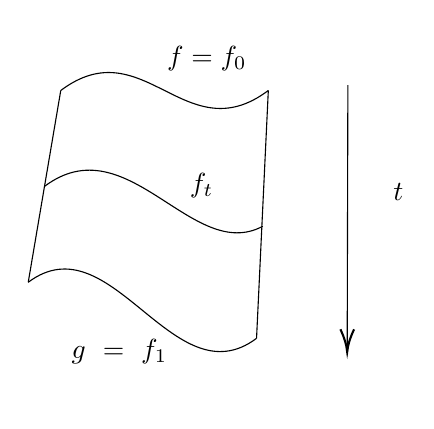
\begin{tikzpicture}[x=0.75pt,y=0.75pt,yscale=-1,xscale=1]
%uncomment if require: \path (0,223); %set diagram left start at 0, and has height of 223

%Curve Lines [id:da9058651841616174] 
\draw    (262,56) .. controls (302,26) and (322,86) .. (362,56) ;
%Straight Lines [id:da0513678676424314] 
\draw    (262,56) -- (246.33,148.4) ;
%Curve Lines [id:da5280458737870739] 
\draw    (246.33,148.4) .. controls (286.33,118.4) and (316.33,205.4) .. (356.33,175.4) ;
%Straight Lines [id:da573147102562708] 
\draw    (362,56) -- (356.33,175.4) ;
%Curve Lines [id:da28783759728665137] 
\draw    (254.17,102.2) .. controls (294.17,72.2) and (325.5,139.6) .. (359.33,121.4) ;
%Straight Lines [id:da27797775903405264] 
\draw    (400.33,53.4) -- (400.01,180) ;
\draw [shift={(400,182)}, rotate = 270.15] [color={rgb, 255:red, 0; green, 0; blue, 0 }  ][line width=0.75]    (10.93,-3.29) .. controls (6.95,-1.4) and (3.31,-0.3) .. (0,0) .. controls (3.31,0.3) and (6.95,1.4) .. (10.93,3.29)   ;

% Text Node
\draw (312,33.4) node [anchor=north west][inner sep=0.75pt]    {$f=f_{0}$};
% Text Node
\draw (266,174.4) node [anchor=north west][inner sep=0.75pt]    {$g\ =\ f_{1}$};
% Text Node
\draw (323,94.4) node [anchor=north west][inner sep=0.75pt]    {$f_{t}$};
% Text Node
\draw (421,99.4) node [anchor=north west][inner sep=0.75pt]    {$t$};


\end{tikzpicture}\]
既然有了同伦这一个关系,并且我们观察同伦关系的符号'$\simeq$',它长得有点像'=',那么我们不仅思考这其中是否有什么联系呢?也就是说,$\simeq$是否表示一个等价关系?


\begin{proposition}
在所有的$X \to Y$的映射组成的集合$Y^X$中,映射的同伦是一种等价关系.
\label{Pro:1.2.2}
\end{proposition}
\begin{proof}
反身性:考虑$F(x,t) = f(x)$即可,对于这个映射有$F(x,0) = f(x)$且$F(x,1) = f(x)$因此同伦关系具有反身性.
\\
对称性:假设$f \simeq g$,因而存在$F(x,t)$使得$F(x,0) = f(x)$且$F(x,1) = g(x)$我们只需要设$G(x,t) = F(x,1-t)$即可.有$G(x,0) = g(x)$且$G(x,1) = f(x)$因此同伦关系具有传递性.
\\
传递性:假设$f \simeq g$且$g \simeq h$,因此存在$F(x,t),G(x,t)$使得$F(x,0) = f(x)$,$F(x,1) = G(x,0) = g(x)$,$G(x,1) = h(x)$因此我们可以考虑构造一个如图所示的$H$
\[\tikzset{every picture/.style={line width=0.75pt}} %set default line width to 0.75pt       
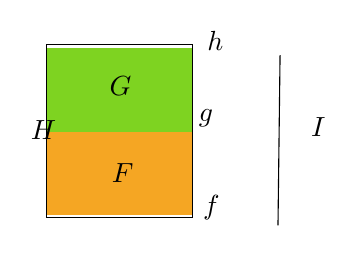
\begin{tikzpicture}[x=0.75pt,y=0.75pt,yscale=-1,xscale=1]
%uncomment if require: \path (0,223); %set diagram left start at 0, and has height of 223

%Shape: Rectangle [id:dp7371205886821253] 
\draw  [color={rgb, 255:red, 245; green, 166; blue, 35 }  ,draw opacity=1 ][fill={rgb, 255:red, 245; green, 166; blue, 35 }  ,fill opacity=1 ] (276,116) -- (346,116) -- (346,156) -- (276,156) -- cycle ;
%Shape: Rectangle [id:dp7309373772723575] 
\draw  [color={rgb, 255:red, 126; green, 211; blue, 33 }  ,draw opacity=1 ][fill={rgb, 255:red, 126; green, 211; blue, 33 }  ,fill opacity=1 ] (276,76) -- (346,76) -- (346,116) -- (276,116) -- cycle ;
%Shape: Rectangle [id:dp18238144249718236] 
\draw   (276,74.4) -- (346,74.4) -- (346,157.4) -- (276,157.4) -- cycle ;
%Straight Lines [id:da5868316488961693] 
\draw    (388.33,79.4) -- (387.33,161.4) ;

% Text Node
\draw (306,130.4) node [anchor=north west][inner sep=0.75pt]    {$F$};
% Text Node
\draw (305,88.4) node [anchor=north west][inner sep=0.75pt]    {$G$};
% Text Node
\draw (352,66.4) node [anchor=north west][inner sep=0.75pt]    {$h$};
% Text Node
\draw (348,104.4) node [anchor=north west][inner sep=0.75pt]    {$g$};
% Text Node
\draw (350,145.4) node [anchor=north west][inner sep=0.75pt]    {$f$};
% Text Node
\draw (402,108.4) node [anchor=north west][inner sep=0.75pt]    {$I$};
% Text Node
\draw (267,109.4) node [anchor=north west][inner sep=0.75pt]    {$H$};
\end{tikzpicture}\]


使得$H$将$F$与$G$"粘接"在了一起,因此可以得到$H$的表达式为
$$
H(x,t)= \left\{
\begin{array}{c}
F(x,2t) , 0 \leq t \leq \frac{1}{2}\\
G(x,2t-1) ,\frac{1}{2}\leq t \leq 1\\
\end{array}
\right.
$$
而后有$H(x,0) = f(x)$,$H(x,1) = h(x)$因此得到$f \simeq h$.即同伦关系具有传递性


因此同伦关系在$Y^X$中是一个等价关系
\end{proof}
得到同伦是一个等价关系后,就可以进一步得到一个重要的引理.
\begin{lemma}
    如果$f_0 \simeq f_1:X\to Y$且$g_0 \simeq g_2 : Y \to Z$是拓扑空间之间同伦的映射,则有$g_0 \circ f_0 \simeq g_1 \circ f_1 : X \to Z$.
    \label{lem:1.2.3}
\end{lemma}

\begin{proof}
    由于命题\ref{Pro:1.2.2}知同伦是一个等价关系,因此只需要证明$g_0 \circ f_0 \simeq g_0 \circ f_1 \circ g_1 \circ f_1$即可.\\
    1. 由于$f_0 \simeq f_1$,存在伦移$F : X \times I \to Y$使得$F : f_0 \simeq f_1$,定义映射
    $$
    H = g_0 \circ F : X \times I \to Z
    $$
    即对任意的$x \in X$,$t \in I$都有$H(x,t) = g_0(F(x,t))$.$H(x,0) = g_0(F(x,0)) = g_0 \circ f_0(x)$,$H(x,1) = g_0 \circ f_1(x)$.这也就证明了$H: g_0 \circ f_0 \simeq g_0 \circ f_1$.\\
    2. 由于$g_0 \simeq g_1$,存在伦移$G : Y \times I \to X$使得$G : g_0 \simeq g_1$,可以定义映射
    $$
    \tilde{H} = G \circ f_1: X \times I \to Z
    $$
    不难验证$\tilde{H}: g_0 \circ f_1 \simeq g_1 \circ f_1$.\\
    据此,就可以根据传递性得到$g_0 \circ f_0 \simeq g_1 \circ f_1$.
\end{proof}

由于等价关系可以在集合中形成一个分划,进而得到一个商集将符合等价关系的元素进行归类,自然地,我们也想对于$Y^X$中关于同伦关系作一个商集.
\begin{definition}
    $Y^X$中关于$\simeq$的商集记为$Y^X / \simeq$
    $$
    Y^X/\simeq := \{[f]: f: X \to Y\}
    $$
    且$[f] := \{g : g \simeq f\}$称$[f]$为同伦等价类.


    一般地,将$Y^X/\simeq$记为$[X,Y]$,称为从$X$到$Y$的同伦类集.
    \label{Def:1.2.2}
\end{definition}

这也就引出了代数拓扑中的另一个中心问题(同伦论):任给拓扑空间$X,Y$,$[X,Y]$中有多少个同伦类?


关于这个问题的研究目前也有一些进展
\begin{example}
    $[S^n ,S^n] \cong \mathbb{Z}$,$[S^3,S^2]\cong \mathbb{Z}$,$[S^4,S^3] \cong \mathbb{Z}_2$
\label{Exa:1.2.3}
\end{example}
既然在例\ref{Exa:1.2.3}中提到了$S^n$的同伦,不妨讨论一下任意一个拓扑空间$X$到$S^n$上的映射同伦关系.
\begin{proposition}
    设$X$为拓扑空间,$S^n$为$n+1$维球面,若存在两个映射$f,g : X \to S^n$,满足$\forall x \in X,f(x) \neq - g(x)$则$f \simeq g$
    \[\tikzset{every picture/.style={line width=0.75pt}} %set default line width to 0.75pt        
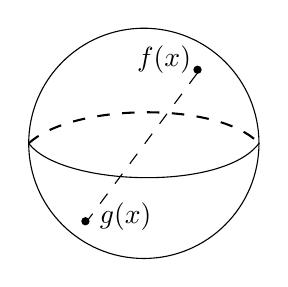
\begin{tikzpicture}[x=0.75pt,y=0.75pt,yscale=-1,xscale=1]
%uncomment if require: \path (0,223); %set diagram left start at 0, and has height of 223

%Shape: Circle [id:dp02705364568316715] 
\draw   (116,100.87) .. controls (116,70.23) and (140.83,45.4) .. (171.47,45.4) .. controls (202.1,45.4) and (226.93,70.23) .. (226.93,100.87) .. controls (226.93,131.5) and (202.1,156.33) .. (171.47,156.33) .. controls (140.83,156.33) and (116,131.5) .. (116,100.87) -- cycle ;
%Curve Lines [id:da6661878225569084] 
\draw [line width=0.75]  [dash pattern={on 4.5pt off 4.5pt}]  (116,100.87) .. controls (137.33,81.4) and (207.33,80.4) .. (226.93,100.87) ;
%Curve Lines [id:da12852557857307922] 
\draw    (116,100.87) .. controls (131.33,121.4) and (209.33,124.4) .. (226.93,100.87) ;
%Straight Lines [id:da8202551406495595] 
\draw  [dash pattern={on 4.5pt off 4.5pt}]  (196.97,67.37) -- (143.33,139.4) ;
%Shape: Free Drawing [id:dp9209610825269543] 
\draw  [line width=3] [line join = round][line cap = round] (197.33,65.4) .. controls (197.33,65.4) and (197.33,65.4) .. (197.33,65.4) ;
%Shape: Free Drawing [id:dp7931907502929314] 
\draw  [line width=3] [line join = round][line cap = round] (143.33,138.4) .. controls (143.33,138.4) and (143.33,138.4) .. (143.33,138.4) ;

% Text Node
\draw (149,128.4) node [anchor=north west][inner sep=0.75pt]    {$g( x)$};
% Text Node
\draw (167,52.4) node [anchor=north west][inner sep=0.75pt]    {$f( x)$};
\end{tikzpicture}\]
    其中$f(x) \neq -g(x)$在$S^2$中如上图所示
\label{Pro:1.2.5}
\end{proposition}
\begin{proof}
    若$f \simeq g$,则存在$F: X\times I \to S^n$使得$f(x) \neq g(x)$,那么不妨设
    $$
    F(x,t) = \frac{(1-t)f(x)+tg(x)}{\|(1-t)f(x)+tg(x)\|}
    $$
    此时若$\|(1-t)f(x) +tg(x)\|\neq 0$就有$F(x,0) = f(x)$且$f(x,1) = g(x)$,$\forall x \in X,F(x,t) \in S^n$.此时显然有$f \simeq g$.


    但是上述过程有一个要求,即$\|(1-t)f(x) +tg(x)\|\neq 0$,也就是说$(1-t) f(x) +tg(x) \neq 0$.若有
    $$
    (1-t)f(x)+tg(x) = 0 \Rightarrow(1-t)f(x) = -tg(x)
    $$
    两边同时取范数得到
    $$
    1-t = t
    $$
    即$t = \frac{1}{2}$.带回原式得到此时$f(x) = -g(x)$.


    因此若$f(x) \neq -g(x)$则必然存在$F(x,t)$使得$f \simeq g$.
\end{proof}



命题\ref{Pro:1.2.5}直接引出了命题\ref{Pro:1.2.6}
\begin{proposition}
若$X$到$S^n$的某个映射不为满射,则它一定同伦于某个常值映射
    \label{Pro:1.2.6}
\end{proposition}
\begin{proof}
    设$f : X \to S^n$不为满射,那么存在$x_0 \in S^n$使得$-x_0 \notin \text{Im }f$


    因此对于任意的$a \in X$都有$f(a) \neq -x_0$.


    根据命题\ref{Pro:1.2.5}可知,若我们设一个函数$g(x)$使得对于任意的$a \in X$都有$g(a) = -x_0$,那么就有$f \simeq g$.


    不难发现这样的$g(x)$就是常值映射$c_{x_0}$.


    因此若$f$不为满射,则其必然同伦于某个常值映射
\end{proof}


有了命题\ref{Pro:1.2.6}后,我们就可以延续例\ref{Exa:1.2.3}的工作了,在例\ref{Exa:1.2.3}中,我们总是考虑$S^n$到$S^m$之间的同伦类个数(其中$n$总是大于$m$).现在我们可以看看$n<m$的情况了.


不难发现,当$n<m$时$S^n \hookrightarrow S^m$为一个嵌入映射,显然不是满射,因此运用命题\ref{Pro:1.2.6}的结论可以得到$[S^n,S^m]$总是只有一个同伦类,即常值映射的同伦类.

\subsubsection{空间同伦}
回忆同胚的定义\ref{Def:0.1.1}.


若$f : X \xrightarrow{\cong}Y$则存在$g : Y \to X$使得
\[\begin{tikzcd}
	X && Y && Y && X \\
	\\
	&& X &&&& Y
	\arrow["g", from=1-3, to=3-3]
	\arrow["f", from=1-1, to=1-3]
	\arrow["{\text{id}_X}"', from=1-1, to=3-3]
	\arrow["g", from=1-5, to=1-7]
	\arrow["f", from=1-7, to=3-7]
	\arrow["{\text{id}_Y}"', from=1-5, to=3-7]
\end{tikzcd}\]
在同胚的意义下,$f\circ g$与$\text{id}_Y$以及$g \circ f$与$\text{id}_X$需要严格相等.


现在,由于我们引入了映射同伦这一观点,我们可以学习范畴中的"以同构代替严格等式",而同伦,就是我们所使用的"同构".这就引出了定义\ref{Def:2.2.3}
\begin{definition}
对于拓扑空间$X,Y$若存在映射$f : X \to Y$,$g : Y \to X$使得$g \circ f \simeq \text{id}_X$且$f \circ g \simeq \text{id}_Y$,即下述图表交换.
\[\begin{tikzcd}
	{(X,A)} && {(Y,B)} && {(Y,B)} && {(X,A)} \\
	\\
	&& {(X,A)} &&&& {(Y,B)} 
	&& {}
	\arrow["g", from=1-3, to=3-3]
	\arrow["f", from=1-1, to=1-3]
	\arrow["{\simeq1_{X}}"', from=1-1, to=3-3]
	\arrow["g", from=1-5, to=1-7]
	\arrow["f", from=1-7, to=3-7]
	\arrow["{\simeq 1_{Y}}"', from=1-5, to=3-7]
\end{tikzcd}\]
则称$X$和$Y$是同伦等价的,或称$X$与$Y$有着相同的伦型,记为$X \simeq Y$或$f : X \xrightarrow{\simeq}Y$.
    \label{Def:1.2.3}
\end{definition}

\subsubsection{空间偶以及空间偶之间的映射}
在具体的研究中,我们常常需要保持拓扑空间$X$的子空间$A$映射到拓扑空间$Y$的子空间$B$上(比如基点).但是对于这样的映射,我们需要使用额外的符号将其表述出来,如果我们记其为$f : A \to B$那就丢失$f$其实是$X \to Y$的映射这一信息,而记$f : X \to Y$又无法体现出$f(A) \subset B$,两者都写就过于繁琐了,因此,拓扑学家参考关系中有序偶这一概念,创造出空间偶来表示一些有这类特殊需求的映射.

\begin{definition}
    设$A$为$X$的一个子空间,则$(X,A)$称为一个空间偶,若$(Y,B)$为另一个空间偶,$f : X \to Y$为一个映射,并且有$f(A) \subset B$则称$f$为空间偶之间的映射,记为$f: (X,A) \to (Y,B)$.
    \label{Def:1.2.4}
\end{definition}

有空间偶上的映射,回想这一节的标题"同伦",那么自然也会想着构建出空间偶映射的同伦了.


空间偶映射之间的同伦该如何构建呢?


我们分几步进行探讨.


首先,对于两个映射,若它们是空间偶映射的同伦,那么它们应当在$X$和$Y$之间互相同伦,即存在伦移$F(x,t)$使得$F(x,0) = f(x)$且$F(x,1) = g(x)$.


其次,先前提到过,同伦映射是一个连续变化的过程,既然是空间偶映射之间的同伦,那么这个连续变化的过程应该限制在空间偶上,即$\forall t \in I$都有$F(A,t) \subset B$.


我们这就得到了空间偶映射之间同伦的定义.


\begin{definition}
    设$f,g : (X,A) \to (Y,B)$为空间偶之间的映射,若存在$F: X \times I \to Y$使得$F(x,0) = f(x)$且$F(x,1) = g(x)$,并且对于任意的$t \in I$都有$F(A,t) \subset B$则称$f$与$g$为空间偶映射的同伦,记为$f\simeq g:(X,A) \to (Y,B)$
\end{definition}

当子空间$A$和$B$坍缩为一个点的时候,我们把这个点称为基点.

\begin{definition}
    取$A = \{x_0\}, B = \{y_0\}$时称$X,Y$为带基点的空间,其中$x_0$为$X$的基点,$y_0$为$Y$的基点.
\end{definition}

类似地,我们可以定义空间偶之间的同伦.

\begin{definition}
    对于空间偶$(X,A)$,$(Y,B)$,若存在$f :(X,A) \to (Y,B)$,$g : (Y,B) \to (X,A)$使得$g \circ f\simeq 1_{(X,A)}$且$f \circ g \simeq 1_{(Y,B)}$即下图交换
    \[\begin{tikzcd}
	{(X,A)} && {(Y,B)} && {(Y,B)} && {(X,A)} \\
	\\
	&& {(X,A)} &&&& {(Y,B)} 
	&& {}
	\arrow["g", from=1-3, to=3-3]
	\arrow["f", from=1-1, to=1-3]
	\arrow["{\simeq1_{(X,A)}}"', from=1-1, to=3-3]
	\arrow["g", from=1-5, to=1-7]
	\arrow["f", from=1-7, to=3-7]
	\arrow["{\simeq 1_{(Y,B)}}"', from=1-5, to=3-7]
\end{tikzcd}\]
则称$(X,A)$与$(Y,B)$是空间偶上同伦等价的.
\end{definition}
\subsubsection{收缩核}
先从一个\sout{栗子}例子开始讲起(这个栗子有点大).
\begin{example}
$\mathbb{R}^2 \setminus\{O\}$与$S^1$是同伦的.


从几何直观上看,无非就是下图
\[\tikzset{every picture/.style={line width=0.75pt}} %set default line width to 0.75pt  
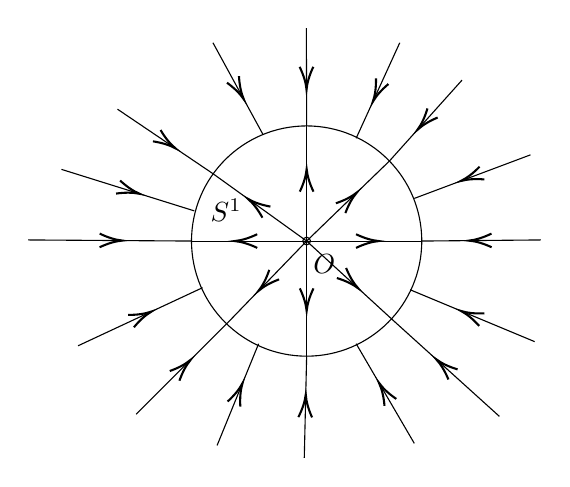
\begin{tikzpicture}[x=0.75pt,y=0.75pt,yscale=-1,xscale=1]
%uncomment if require: \path (0,223); %set diagram left start at 0, and has height of 223

%Shape: Circle [id:dp02705364568316715] 
\draw   (116,100.87) .. controls (116,70.23) and (140.83,45.4) .. (171.47,45.4) .. controls (202.1,45.4) and (226.93,70.23) .. (226.93,100.87) .. controls (226.93,131.5) and (202.1,156.33) .. (171.47,156.33) .. controls (140.83,156.33) and (116,131.5) .. (116,100.87) -- cycle ;
%Straight Lines [id:da33415538965340863] 
\draw    (126.33,68.4) -- (171.47,100.87) ;
\draw [shift={(143.22,80.55)}, rotate = 35.73] [color={rgb, 255:red, 0; green, 0; blue, 0 }  ][line width=0.75]    (10.93,-3.29) .. controls (6.95,-1.4) and (3.31,-0.3) .. (0,0) .. controls (3.31,0.3) and (6.95,1.4) .. (10.93,3.29)   ;
%Straight Lines [id:da4368346628206423] 
\draw    (171.47,45.4) -- (171.47,100.87) ;
\draw [shift={(171.47,66.13)}, rotate = 90] [color={rgb, 255:red, 0; green, 0; blue, 0 }  ][line width=0.75]    (10.93,-3.29) .. controls (6.95,-1.4) and (3.31,-0.3) .. (0,0) .. controls (3.31,0.3) and (6.95,1.4) .. (10.93,3.29)   ;
%Straight Lines [id:da24485194473395677] 
\draw    (226.93,100.87) -- (171.47,100.87) ;
\draw [shift={(206.2,100.87)}, rotate = 180] [color={rgb, 255:red, 0; green, 0; blue, 0 }  ][line width=0.75]    (10.93,-3.29) .. controls (6.95,-1.4) and (3.31,-0.3) .. (0,0) .. controls (3.31,0.3) and (6.95,1.4) .. (10.93,3.29)   ;
%Straight Lines [id:da007751330948918778] 
\draw    (171.47,100.87) -- (211.33,62.33) ;
\draw [shift={(195.71,77.43)}, rotate = 135.97] [color={rgb, 255:red, 0; green, 0; blue, 0 }  ][line width=0.75]    (10.93,-3.29) .. controls (6.95,-1.4) and (3.31,-0.3) .. (0,0) .. controls (3.31,0.3) and (6.95,1.4) .. (10.93,3.29)   ;
%Straight Lines [id:da7197695599626932] 
\draw    (116,100.87) -- (171.47,100.87) ;
\draw [shift={(136.73,100.87)}, rotate = 0] [color={rgb, 255:red, 0; green, 0; blue, 0 }  ][line width=0.75]    (10.93,-3.29) .. controls (6.95,-1.4) and (3.31,-0.3) .. (0,0) .. controls (3.31,0.3) and (6.95,1.4) .. (10.93,3.29)   ;
%Straight Lines [id:da02885928058013909] 
\draw    (171.47,100.87) -- (133.33,140.33) ;
\draw [shift={(148.23,124.91)}, rotate = 314.02] [color={rgb, 255:red, 0; green, 0; blue, 0 }  ][line width=0.75]    (10.93,-3.29) .. controls (6.95,-1.4) and (3.31,-0.3) .. (0,0) .. controls (3.31,0.3) and (6.95,1.4) .. (10.93,3.29)   ;
%Straight Lines [id:da6571891557883147] 
\draw    (171.47,100.87) -- (171.47,156.33) ;
\draw [shift={(171.47,134.6)}, rotate = 270] [color={rgb, 255:red, 0; green, 0; blue, 0 }  ][line width=0.75]    (10.93,-3.29) .. controls (6.95,-1.4) and (3.31,-0.3) .. (0,0) .. controls (3.31,0.3) and (6.95,1.4) .. (10.93,3.29)   ;
%Straight Lines [id:da6782459906432647] 
\draw    (171.47,100.87) -- (212.33,138.33) ;
\draw [shift={(196.32,123.65)}, rotate = 222.51] [color={rgb, 255:red, 0; green, 0; blue, 0 }  ][line width=0.75]    (10.93,-3.29) .. controls (6.95,-1.4) and (3.31,-0.3) .. (0,0) .. controls (3.31,0.3) and (6.95,1.4) .. (10.93,3.29)   ;
%Straight Lines [id:da3885143598329224] 
\draw    (80.33,37.33) -- (126.33,68.4) ;
\draw [shift={(108.31,56.22)}, rotate = 214.03] [color={rgb, 255:red, 0; green, 0; blue, 0 }  ][line width=0.75]    (10.93,-3.29) .. controls (6.95,-1.4) and (3.31,-0.3) .. (0,0) .. controls (3.31,0.3) and (6.95,1.4) .. (10.93,3.29)   ;
%Straight Lines [id:da8554099683385705] 
\draw    (37.33,100.33) -- (116,100.87) ;
\draw [shift={(82.67,100.64)}, rotate = 180.39] [color={rgb, 255:red, 0; green, 0; blue, 0 }  ][line width=0.75]    (10.93,-3.29) .. controls (6.95,-1.4) and (3.31,-0.3) .. (0,0) .. controls (3.31,0.3) and (6.95,1.4) .. (10.93,3.29)   ;
%Straight Lines [id:da764625353687989] 
\draw    (53.33,66.33) -- (117.33,86.33) ;
\draw [shift={(91.06,78.12)}, rotate = 197.35] [color={rgb, 255:red, 0; green, 0; blue, 0 }  ][line width=0.75]    (10.93,-3.29) .. controls (6.95,-1.4) and (3.31,-0.3) .. (0,0) .. controls (3.31,0.3) and (6.95,1.4) .. (10.93,3.29)   ;
%Straight Lines [id:da06864025772560778] 
\draw    (126.33,5.33) -- (150.33,49.33) ;
\draw [shift={(141.21,32.6)}, rotate = 241.39] [color={rgb, 255:red, 0; green, 0; blue, 0 }  ][line width=0.75]    (10.93,-3.29) .. controls (6.95,-1.4) and (3.31,-0.3) .. (0,0) .. controls (3.31,0.3) and (6.95,1.4) .. (10.93,3.29)   ;
%Straight Lines [id:da09891123110701128] 
\draw    (171.33,-1.67) -- (171.47,45.4) ;
\draw [shift={(171.42,27.87)}, rotate = 269.84] [color={rgb, 255:red, 0; green, 0; blue, 0 }  ][line width=0.75]    (10.93,-3.29) .. controls (6.95,-1.4) and (3.31,-0.3) .. (0,0) .. controls (3.31,0.3) and (6.95,1.4) .. (10.93,3.29)   ;
%Straight Lines [id:da32941276629096405] 
\draw    (216.33,5.33) -- (195.33,51.33) ;
\draw [shift={(203.34,33.79)}, rotate = 294.54] [color={rgb, 255:red, 0; green, 0; blue, 0 }  ][line width=0.75]    (10.93,-3.29) .. controls (6.95,-1.4) and (3.31,-0.3) .. (0,0) .. controls (3.31,0.3) and (6.95,1.4) .. (10.93,3.29)   ;
%Straight Lines [id:da9532074975088578] 
\draw    (246.33,23.33) -- (211.33,62.33) ;
\draw [shift={(224.83,47.3)}, rotate = 311.91] [color={rgb, 255:red, 0; green, 0; blue, 0 }  ][line width=0.75]    (10.93,-3.29) .. controls (6.95,-1.4) and (3.31,-0.3) .. (0,0) .. controls (3.31,0.3) and (6.95,1.4) .. (10.93,3.29)   ;
%Straight Lines [id:da6563564089799596] 
\draw    (279.33,59.33) -- (223.33,80.33) ;
\draw [shift={(245.72,71.94)}, rotate = 339.44] [color={rgb, 255:red, 0; green, 0; blue, 0 }  ][line width=0.75]    (10.93,-3.29) .. controls (6.95,-1.4) and (3.31,-0.3) .. (0,0) .. controls (3.31,0.3) and (6.95,1.4) .. (10.93,3.29)   ;
%Straight Lines [id:da9340859427257695] 
\draw    (284.33,100.33) -- (226.93,100.87) ;
\draw [shift={(249.63,100.66)}, rotate = 359.47] [color={rgb, 255:red, 0; green, 0; blue, 0 }  ][line width=0.75]    (10.93,-3.29) .. controls (6.95,-1.4) and (3.31,-0.3) .. (0,0) .. controls (3.31,0.3) and (6.95,1.4) .. (10.93,3.29)   ;
%Straight Lines [id:da32152909509991234] 
\draw    (61.33,151.33) -- (121.33,123.33) ;
\draw [shift={(96.77,134.8)}, rotate = 154.98] [color={rgb, 255:red, 0; green, 0; blue, 0 }  ][line width=0.75]    (10.93,-3.29) .. controls (6.95,-1.4) and (3.31,-0.3) .. (0,0) .. controls (3.31,0.3) and (6.95,1.4) .. (10.93,3.29)   ;
%Straight Lines [id:da5361579046466207] 
\draw    (89.33,184.33) -- (133.33,140.33) ;
\draw [shift={(115.58,158.09)}, rotate = 135] [color={rgb, 255:red, 0; green, 0; blue, 0 }  ][line width=0.75]    (10.93,-3.29) .. controls (6.95,-1.4) and (3.31,-0.3) .. (0,0) .. controls (3.31,0.3) and (6.95,1.4) .. (10.93,3.29)   ;
%Straight Lines [id:da6579783410694615] 
\draw    (128.33,199.33) -- (148.33,150.33) ;
\draw [shift={(140.6,169.28)}, rotate = 112.2] [color={rgb, 255:red, 0; green, 0; blue, 0 }  ][line width=0.75]    (10.93,-3.29) .. controls (6.95,-1.4) and (3.31,-0.3) .. (0,0) .. controls (3.31,0.3) and (6.95,1.4) .. (10.93,3.29)   ;
%Straight Lines [id:da14654337096112102] 
\draw    (170.33,205.33) -- (171.47,156.33) ;
\draw [shift={(171.04,174.83)}, rotate = 91.32] [color={rgb, 255:red, 0; green, 0; blue, 0 }  ][line width=0.75]    (10.93,-3.29) .. controls (6.95,-1.4) and (3.31,-0.3) .. (0,0) .. controls (3.31,0.3) and (6.95,1.4) .. (10.93,3.29)   ;
%Straight Lines [id:da6401364858477188] 
\draw    (223.33,198.33) -- (195.33,150.33) ;
\draw [shift={(206.31,169.15)}, rotate = 59.74] [color={rgb, 255:red, 0; green, 0; blue, 0 }  ][line width=0.75]    (10.93,-3.29) .. controls (6.95,-1.4) and (3.31,-0.3) .. (0,0) .. controls (3.31,0.3) and (6.95,1.4) .. (10.93,3.29)   ;
%Straight Lines [id:da41211560416533355] 
\draw    (264.33,185.33) -- (212.33,138.33) ;
\draw [shift={(233.88,157.81)}, rotate = 42.11] [color={rgb, 255:red, 0; green, 0; blue, 0 }  ][line width=0.75]    (10.93,-3.29) .. controls (6.95,-1.4) and (3.31,-0.3) .. (0,0) .. controls (3.31,0.3) and (6.95,1.4) .. (10.93,3.29)   ;
%Straight Lines [id:da9684292220825628] 
\draw    (281.33,149.33) -- (221.33,124.33) ;
\draw [shift={(245.79,134.53)}, rotate = 22.62] [color={rgb, 255:red, 0; green, 0; blue, 0 }  ][line width=0.75]    (10.93,-3.29) .. controls (6.95,-1.4) and (3.31,-0.3) .. (0,0) .. controls (3.31,0.3) and (6.95,1.4) .. (10.93,3.29)   ;
%Shape: Circle [id:dp5246914707050254] 
\draw   (169.61,100.87) .. controls (169.61,99.84) and (170.44,99.01) .. (171.47,99.01) .. controls (172.49,99.01) and (173.32,99.84) .. (173.32,100.87) .. controls (173.32,101.89) and (172.49,102.72) .. (171.47,102.72) .. controls (170.44,102.72) and (169.61,101.89) .. (169.61,100.87) -- cycle ;

% Text Node
\draw (173.47,106.12) node [anchor=north west][inner sep=0.75pt]    {$O$};
% Text Node
\draw (124,79.4) node [anchor=north west][inner sep=0.75pt]    {$S^{1}$};
\end{tikzpicture}\]
    首先,不难发现存在一个$S^1 \hookrightarrow \mathbb{R}^2 \setminus\{O\}$的包含映射$\iota$.


    而后,使用极坐标来表示$\mathbb{R}^2$上的点,可以将$\mathbb{R}^2 \setminus\{O\}$表示为
    $$
    \mathbb{R}\setminus\{O\} = \{(r,\theta): 0 < r <+\infty,0\leq \theta <2\pi\}
    $$
    因此可以得到一个$f : \mathbb{R}^2 \to S^1$即
    \begin{eqnarray*}
        f : \mathbb{R}^2\setminus\{O\} &\to& S^1\\
        (r,\theta) &\mapsto& (1,\theta)
        \end{eqnarray*}
    因此可以得到
    \[\begin{tikzcd}
	{S^1} && {\mathbb{R}^2\setminus\{O\}} && {\mathbb{R}^2\setminus\{O\}} && {S^1} \\
	\\
	&& {S^1} &&&& {\mathbb{R}^2\setminus\{O\}} 
	&& {}
	\arrow["f", from=1-3, to=3-3]
	\arrow["\iota", from=1-1, to=1-3]
	\arrow["{1_{S}}"', from=1-1, to=3-3]
	\arrow["f", from=1-5, to=1-7]
	\arrow["\iota", from=1-7, to=3-7]
	\arrow["{?}"', from=1-5, to=3-7]
\end{tikzcd}\]
    即$f \circ \iota = 1_S$,但是我们目前不知道$\iota \circ f$是什么样的(所以打个问号).
    不难发现$\iota \circ f(r,\theta) = (1,\theta) \in \mathbb{R}^2 \setminus \{O\}$
    因此可以构造
    \begin{eqnarray*}
        F : \mathbb{R}^2\setminus\{O\}\times I &\to& \mathbb{R}^2 \setminus\{O\}\\
        ((r,\theta),t) &\mapsto& ((1-t)r+t,\theta)
        \end{eqnarray*}
        可以发现$F((r,\theta),0) = (r,\theta) = 1_{\mathbb{R}^2\setminus\{O\}}$,且$F((r,\theta),1) = \iota \circ f(r,\theta)$,即
        \[\begin{tikzcd}
	&& {\mathbb{R}^2\setminus\{O\}} && {S^1} \\
	\\
	&&&& {\mathbb{R}^2\setminus\{O\}} 
	{}
	\arrow["f", from=1-3, to=1-5]
	\arrow["\iota", from=1-5, to=3-5]
	\arrow["{\simeq 1_{\mathbb{R}^2\setminus\{O\}}}"', from=1-3, to=3-5]
\end{tikzcd}\]
    \label{Exa:2.2.4}
\end{example}

接下来我们把例\ref{Exa:2.2.4}中$f \circ \iota = 1_S$以及$\iota \circ f \simeq 1_{\mathbb{R}^2 \setminus\{O\}}$这一特点刻画出来.
\begin{definition}
    设$A$为$X$的子空间,若存在$r : X \to A$,使得$r \circ \iota$为一个单位映射,即
    \[\begin{tikzcd}
	A && X \\
	\\
	&& A
	\arrow["\iota", from=1-1, to=1-3]
	\arrow["r", from=1-3, to=3-3]
	\arrow["{\text{id}_A}"', from=1-1, to=3-3]
\end{tikzcd}\]
则称$A$是$X$的收缩核.


更进一步,若$\iota \circ r \simeq \text{id}_X$,即
\[\begin{tikzcd}
	X && A \\
	\\
	&& X
	\arrow["r", from=1-1, to=1-3]
	\arrow["\iota", from=1-3, to=3-3]
	\arrow["{\simeq \text{id}_X}"', from=1-1, to=3-3]
\end{tikzcd}\]
则称$A$是$X$的形变收缩核.


如果在伦移过程中$A$不发生改变,则$A$为$X$的强形变收缩核.
\label{Def:2.2.8}
\end{definition}
如果一个空间$X$可以收缩到某一个点上,这类特殊的空间又有着单独的叫法.
\begin{definition}
    若空间$X$同伦等价于一个独点空间$\{pt\}$则称$X$为一个可收缩空间.
\end{definition}
\begin{example}
    $D^2 \simeq \{0\}$
\end{example}
\subsection{常见的拓扑空间}
\subsubsection{商空间}
\begin{definition}
    设$(X,\mathscr{T})$为一个拓扑空间,$\simeq$为$X$上的一个等价关系,记$X/\simeq$为$X$关于$\simeq$的商集.从而可以定义在$X/\simeq$上的拓扑$\mathscr{T}/\simeq$,其中$W\subset X/\simeq$为一个开集当且仅当$\pi^{-1}(W)$为$X$中的一个开集,其中$\pi : X \to X/\simeq$为一个自然射影.
\end{definition}
乍一看有点抽象,我们可以通过几个例子进行一番深入了解,读者可能需要准备一个矩形小纸片进行一点点小实验.
\begin{example}
    考虑$\mathbb{R}^{n+1}\setminus\{0\}$中的等价关系$\sim$


    对于$\mathbb{R}^{n+1}\setminus\{0\}$中的点$x = (x_1,x_2,\cdots,x_{n+1})$以及$y = (y_1,y_2,\cdots,y_{n+1})$,构建等价关系$x \sim y \Leftrightarrow \exists k \in \mathbb{R}\setminus\{0\}, x = ky$.(等价性交由读者进行验证)


    可以依照$\sim$构建一个商空间$\mathbb{R}^{n+1}\setminus\{0\}/\sim$,称其为一个$n$维实射影空间,记为$\mathbb{R}P^n$.其内元素,记为$[x_1,x_2,\cdots,x_{n+1}]$,表示$x = (x_1,x_2,\cdots,x_{n+1})$所在的等价类.从而有$[x_1,x_2,\cdots,x_{n+1}] = [\frac{x_1}{\|x\|},\frac{x_2}{\|x\|},\cdots,\frac{x_{n+1}}{\|x\|}]$为$\frac{x}{\|x\|}$的等价类,而$\frac{x}{\|x\|}\in S^n$因此可以得到一个结论:$\mathbb{R}P^n = S^n /\sim$,其中$x \sim -x$
\end{example}
\subsubsection{粘接}
为什么我们要引入一个商空间这种看起来很多余的概念呢?这是为了将一个或者多个空间依照某种等价关系"粘"起来.这听起来也挺抽象的,通过几个常见的粘接例子可以辅助进行理解这一概念.
\begin{example}
    在$I \times I$中定义等价关系$(t,0)\sim (1-t,0)$其它的点$(s,t)$只与自身等价.
    \[\tikzset{every picture/.style={line width=0.75pt}} %set default line width to 0.75pt     
\begin{tikzpicture}[x=0.75pt,y=0.75pt,yscale=-1,xscale=1]
%uncomment if require: \path (0,223); %set diagram left start at 0, and has height of 223

%Straight Lines [id:da744594172299702] 
\draw    (100,150) -- (210.11,149.35) ;
\draw [shift={(212.11,149.33)}, rotate = 179.66] [color={rgb, 255:red, 0; green, 0; blue, 0 }  ][line width=0.75]    (10.93,-3.29) .. controls (6.95,-1.4) and (3.31,-0.3) .. (0,0) .. controls (3.31,0.3) and (6.95,1.4) .. (10.93,3.29)   ;
%Straight Lines [id:da2026484697551596] 
\draw    (100,150) -- (100,107) -- (100,43) ;
\draw [shift={(100,41)}, rotate = 90] [color={rgb, 255:red, 0; green, 0; blue, 0 }  ][line width=0.75]    (10.93,-3.29) .. controls (6.95,-1.4) and (3.31,-0.3) .. (0,0) .. controls (3.31,0.3) and (6.95,1.4) .. (10.93,3.29)   ;
%Straight Lines [id:da24709043996031] 
\draw    (101,100) -- (151,100) ;
%Straight Lines [id:da8223606114591986] 
\draw    (151,100) -- (151,150) ;
%Shape: Free Drawing [id:dp5336292476876534] 
\draw  [line width=3] [line join = round][line cap = round] (100,138) .. controls (100,138) and (100,138) .. (100,138) ;
%Shape: Free Drawing [id:dp8062657120487398] 
\draw  [line width=3] [line join = round][line cap = round] (151,112) .. controls (151,112) and (151,112) .. (151,112) ;

% Text Node
\draw (87,131.4) node [anchor=north west][inner sep=0.75pt]    {$t$};
% Text Node
\draw (153,103.4) node [anchor=north west][inner sep=0.75pt]    {$1-t$};
% Text Node
\draw (88,29.4) node [anchor=north west][inner sep=0.75pt]    {$t$};
% Text Node
\draw (199,153.4) node [anchor=north west][inner sep=0.75pt]    {$s$};
% Text Node
\draw (90,81.4) node [anchor=north west][inner sep=0.75pt]    {$1$};
% Text Node
\draw (153,153.4) node [anchor=north west][inner sep=0.75pt]    {$1$};
\end{tikzpicture}\]
那么$I \times I/\sim$就是将上图中$(0,t)$和$(1,1-t)$给"粘"起来,也称为将$I \times \{0\}$与$I \times \{1\}$的反方向粘接.其图像为
\[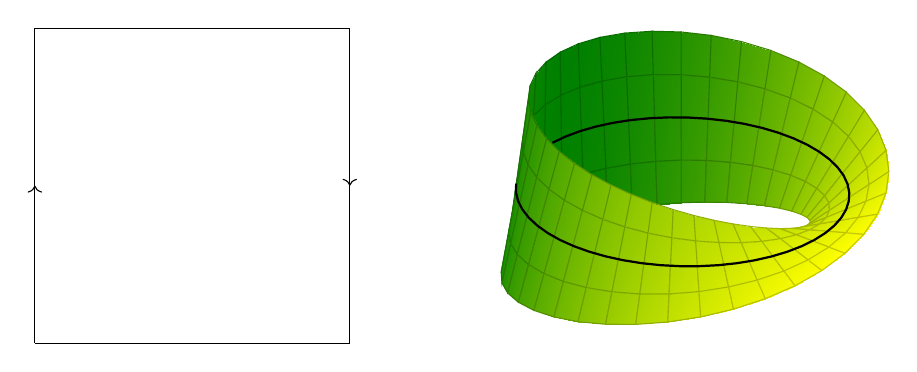
\begin{tikzpicture}[
decoration={
  markings,
  mark=at position 0.5 with {\arrow{>}}}
] 
\draw (-5,5) -- (-1,5);
\draw [postaction=decorate](-1,5) -- (-1,1);
\draw (-1,1) -- (-5,1);
\draw [postaction=decorate](-5,1) -- (-5,5);
\begin{axis}[
hide axis,
view={40}{40}
]
\addplot3 [
surf, shader=faceted interp,
point meta=x,
colormap/greenyellow,
samples=40,
samples y=5,
z buffer=sort,
domain=0:360,
y domain=-0.5:0.5
] (
{(1+0.5*y*cos(x/2)))*cos(x)},
{(1+0.5*y*cos(x/2)))*sin(x)},
{0.5*y*sin(x/2)});

\addplot3 [
samples=50,
domain=-145:180, % The domain needs to be adjusted manually, depending on the camera angle, unfortunately
samples y=0,
thick
] (
{cos(x)},
{sin(x)},
{0});
\end{axis}

\end{tikzpicture}
\]
其中左图为多边形表示(即沿着什么方向进行粘接,粘接起来就是将那两个箭头按照相同的方向黏在一起),右图为粘接后的图像(即一个M\"{o}bius环带)
\end{example}
下一个例子也是对于$I \times I$进行操作.
\begin{example}
    将$I \times I$中的$I \times \{0\}$与$I\times \{1\}$以及$\{0\}\times I$与$\{1\}\times I$都进行正方形粘接,其多边形表示为
    \[\begin{tikzpicture}[
decoration={
  markings,
  mark=at position 0.5 with {\arrow{>}}}
] 
\draw [postaction=decorate](-1,5) -- (-5,5);
\draw [postaction=decorate](-1,5) -- (-1,1);
\draw [postaction=decorate](-1,1) -- (-5,1);
\draw [postaction=decorate](-5,5) -- (-5,1);
\end{tikzpicture}\]
这就是我们常见的一个环带
\[\tikzset{every picture/.style={line width=0.75pt}} %set default line width to 0.75pt        
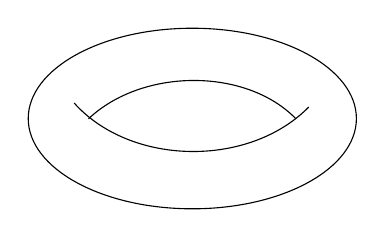
\begin{tikzpicture}[x=0.75pt,y=0.75pt,yscale=-1,xscale=1]
%uncomment if require: \path (0,300); %set diagram left start at 0, and has height of 300

%Curve Lines [id:da5145833269320492] 
\draw    (100,105) .. controls (126.11,80.33) and (176.11,80.33) .. (200,105) ;
%Curve Lines [id:da174982256536782] 
\draw    (93.11,97.33) .. controls (120.22,127.67) and (177.22,128.67) .. (206.11,99.33) ;
%Shape: Ellipse [id:dp9908711578508085] 
\draw   (71,104.83) .. controls (71,80.81) and (106.39,61.33) .. (150.06,61.33) .. controls (193.72,61.33) and (229.11,80.81) .. (229.11,104.83) .. controls (229.11,128.86) and (193.72,148.33) .. (150.06,148.33) .. controls (106.39,148.33) and (71,128.86) .. (71,104.83) -- cycle ;
\end{tikzpicture}\]
$I \times I/\sim$就是上述环带,记为$T$不难发现它无非就是$S^1 \times S^1$
\end{example}
我们已经考虑了对于小卡片$I \times I$的两种粘接方法了,接下来还有一种粘接方法
\begin{example}
    将$I \times I$中,$I \times \{0\}$与$I \times \{1\}$进行反方向粘接,而将$\{0\}\times I$与$\{1\}\times I$进行正方向粘接.得到的多边形表示以及图像为
     \[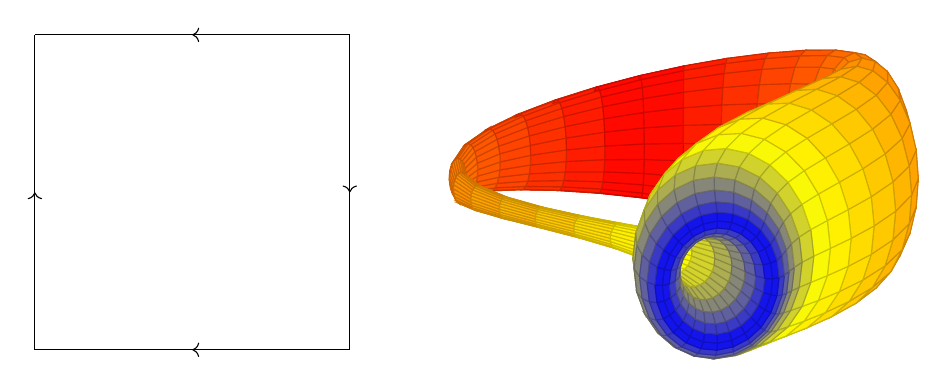
\begin{tikzpicture}[
decoration={
  markings,
  mark=at position 0.5 with {\arrow{>}}}
] 
\draw [postaction=decorate](-1,5) -- (-5,5);
\draw [postaction=decorate](-1,5) -- (-1,1);
\draw [postaction=decorate](-1,1) -- (-5,1);
\draw [postaction=decorate](-5,1) -- (-5,5);
	\begin{axis}[
		xlabel=$x$,
		ylabel=$y$,
		view/h=-10,
       hide axis,
	]
	\addplot3[
		surf,
		z buffer=sort,
		colormap={periodic}{%
			color=(blue) 
			   color=(yellow) 
			      color=(orange) 
				     color=(red)
			      color=(orange) 
	           color=(yellow) 
	        color=(blue)},
		domain=0:180, domain y=0:360,
		samples=41, samples y=25,
		variable=\u, variable y=\v,
		point meta=u,
		] 
		({-2/15 * cos(u) * (
		    3*cos(v) - 30*sin(u) 
		  + 90 *cos(u)^4 * sin(u) 
		  - 60 *cos(u)^6 * sin(u)  
		  + 5 * cos(u)*cos(v) * sin(u))
		 },
		 {-1/15 * sin(u) * (3*cos(v) 
		  - 3*cos(u)^2 * cos(v) 
		  - 48 * cos(u)^4*cos(v) 
		  + 48*cos(u)^6 *cos(v) 
		  - 60 *sin(u) 
		  + 5*cos(u)*cos(v)*sin(u) 
		  - 5*cos(u)^3 * cos(v) *sin(u) 
		  - 80*cos(u)^5 * cos(v)*sin(u) 
		  + 80*cos(u)^7 * cos(v) * sin(u))
		 },
		 {2/15 * (3 + 5*cos(u) *sin(u))*sin(v)});
	\end{axis}
\end{tikzpicture}\]
$I \times I$就是我们常说的Klein瓶.
\end{example}
粘接行为显然不仅仅适用于小纸片$I \times I$上.
\begin{example}
    设$X$为一个拓扑空间,将$X \times I$中$X \times\{1\}$粘接为一个点.
    \[\tikzset{every picture/.style={line width=0.75pt}} %set default line width to 0.75pt    
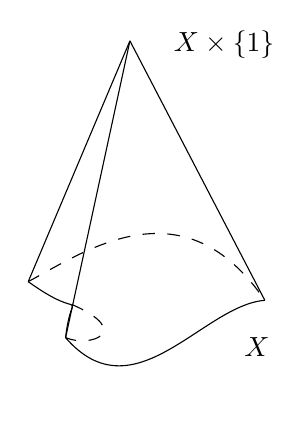
\begin{tikzpicture}[x=0.75pt,y=0.75pt,yscale=-1,xscale=1]
%uncomment if require: \path (0,246); %set diagram left start at 0, and has height of 246

%Curve Lines [id:da6444277677637305] 
\draw  [dash pattern={on 4.5pt off 4.5pt}]  (111.11,138.49) .. controls (139.11,123.49) and (186.11,90.49) .. (225.11,147.49) ;
%Curve Lines [id:da15933269378180293] 
\draw    (225.11,147.49) .. controls (195.22,149.83) and (162.11,203.49) .. (129.11,165.49) ;
%Straight Lines [id:da8713805055011097] 
\draw    (129.11,165.49) -- (160.11,22.49) ;
%Straight Lines [id:da5739490745379057] 
\draw    (160.11,22.49) -- (225.11,147.49) ;
%Straight Lines [id:da9424186414524165] 
\draw    (111.11,138.49) -- (160.11,22.49) ;
%Curve Lines [id:da06020756766297719] 
\draw    (111.11,138.49) .. controls (140.11,159.49) and (132.11,138.49) .. (129.11,165.49) ;
%Curve Lines [id:da6518113912028751] 
\draw  [dash pattern={on 4.5pt off 4.5pt}]  (132.11,149.49) .. controls (162.11,162.49) and (141.11,170.49) .. (129.11,165.49) ;

% Text Node
\draw (214,164.4) node [anchor=north west][inner sep=0.75pt]    {$X$};
% Text Node
\draw (180,16.4) node [anchor=north west][inner sep=0.75pt]    {$X\times \{1\}$};
\end{tikzpicture}\]
称其为一个锥体,记为$CX$,$X \times I$到$CX$的映射为一个射影映射$X \times I \to X \times I/\sim$,因此可以定义射影$\pi : X \times I \to CX$.不难发现$CX\simeq\{pt\}$.当$X = S^1$时,有$CS^1 \cong D^2$.(注意此处为$S^1$而不是$D^2$,它不包含底面).


此外,还可以将$X\times I$中$X \times \{0\}$与$X \times \{1\}$均粘接为一点(即$(x,0)\sim (y,0)$且$(x,1) \simeq (y,1)$,得到的空间形如
  \[ \tikzset{every picture/.style={line width=0.75pt}} %set default line width to 0.75pt        
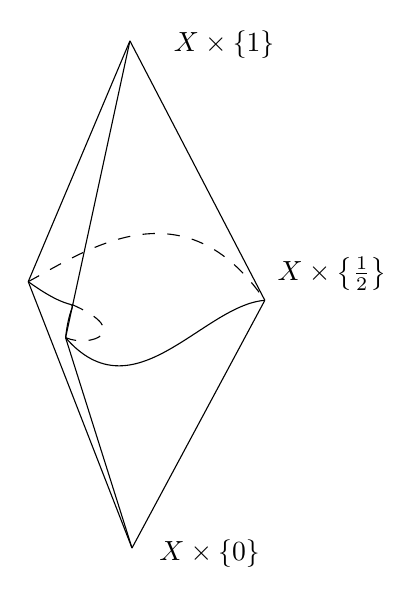
\begin{tikzpicture}[x=0.75pt,y=0.75pt,yscale=-1,xscale=1]
%uncomment if require: \path (0,333); %set diagram left start at 0, and has height of 333

%Curve Lines [id:da6444277677637305] 
\draw  [dash pattern={on 4.5pt off 4.5pt}]  (111.11,138.49) .. controls (139.11,123.49) and (186.11,90.49) .. (225.11,147.49) ;
%Curve Lines [id:da15933269378180293] 
\draw    (225.11,147.49) .. controls (195.22,149.83) and (162.11,203.49) .. (129.11,165.49) ;
%Straight Lines [id:da8713805055011097] 
\draw    (129.11,165.49) -- (160.11,22.49) ;
%Straight Lines [id:da5739490745379057] 
\draw    (160.11,22.49) -- (225.11,147.49) ;
\draw    (111.11,138.49) -- (160.11,22.49) ;
%Curve Lines [id:da06020756766297719] 
\draw    (111.11,138.49) .. controls (140.11,159.49) and (132.11,138.49) .. (129.11,165.49) ;
%Curve Lines [id:da6518113912028751] 
\draw  [dash pattern={on 4.5pt off 4.5pt}]  (132.11,149.49) .. controls (162.11,162.49) and (141.11,170.49) .. (129.11,165.49) ;
%Straight Lines [id:da2877261911804203] 
\draw    (111.11,138.49) -- (161.11,266.83) ;
%Straight Lines [id:da4298131926737394] 
\draw    (129.11,165.49) -- (161.11,266.83) ;
%Straight Lines [id:da22416750291611787] 
\draw    (225.11,147.49) -- (161.11,266.83) ;

% Text Node
\draw (230,125.4) node [anchor=north west][inner sep=0.75pt]    {$X\times \left\{\frac{1}{2}\right\}$};
% Text Node
\draw (180,16.4) node [anchor=north west][inner sep=0.75pt]    {$X\times \{1\}$};
% Text Node
\draw (173,261.4) node [anchor=north west][inner sep=0.75pt]    {$X\times \{0\}$};
\end{tikzpicture}\]
我们称其为$X$的一个双角锥,记为$\Sigma X$.不难发现$\Sigma S^1 \cong S^2$.
\end{example}
根据前面的4个例子,想必读者已然可以得出粘接的具体含义:即通过某种等价关系将空间中的某些区域进行粘合.接着就可以给出粘接的具体定义了
\begin{definition}
    设$A$为$X$的子空间,$f : A \times Y$在$X \sqcup Y$中定义等价关系$\sim$:对于任意的$a \in A$,$a \sim f(a)$.其它的点只与子集等价.得到的商空间$X \sqcup Y /\sim$称为将$X$沿着映射$f : A \to Y$粘合在$Y$上,记为$Y \cup_{f}X$
\end{definition}
注意,粘合是一个有序的过程,$Y \cup _f X$是将$X$粘合在$Y$上,$\cup$两侧的顺序是不能像集合一样随意调换的.


前文我们所介绍的粘接概念都是一个空间$X$与自身的粘接,接下来给出两个空间之间的粘接
\begin{example}
    设$f : X \to Y$,考虑$CX$中子空间$X \times \{0\}$到$Y$的映射
    \begin{eqnarray*}
        \tilde{f}: X \times \{0\} &\to& Y\\
        (x,0) &\mapsto& f(x)
    \end{eqnarray*}
    使用$\tilde{f}$将$CX$粘接在$Y$上,即$CX$沿$\tilde{f}: X \times \{0\} \to Y$粘接在$Y$上.


    得到的空间记为$Y \cup_{f} CX$,称为一个$f : X \to Y$的映射锥,不难发现$Y\hookrightarrow Y \cup_{f} CX$.


    比方说取$X = S^1$时,$f : S^1 \times Y$的映射锥为
    \[\tikzset{every picture/.style={line width=0.75pt}} %set default line width to 0.75pt   
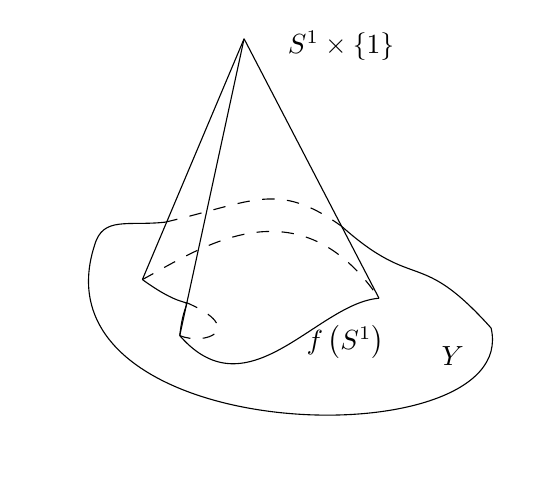
\begin{tikzpicture}[x=0.75pt,y=0.75pt,yscale=-1,xscale=1]
%uncomment if require: \path (0,333); %set diagram left start at 0, and has height of 333

%Curve Lines [id:da6444277677637305] 
\draw  [dash pattern={on 4.5pt off 4.5pt}]  (111.11,138.49) .. controls (139.11,123.49) and (186.11,90.49) .. (225.11,147.49) ;
%Curve Lines [id:da15933269378180293] 
\draw    (225.11,147.49) .. controls (195.22,149.83) and (162.11,203.49) .. (129.11,165.49) ;
%Straight Lines [id:da8713805055011097] 
\draw    (129.11,165.49) -- (160.11,22.49) ;
%Straight Lines [id:da5739490745379057] 
\draw    (160.11,22.49) -- (225.11,147.49) ;
%Straight Lines [id:da9424186414524165] 
\draw    (111.11,138.49) -- (160.11,22.49) ;
%Curve Lines [id:da06020756766297719] 
\draw    (111.11,138.49) .. controls (140.11,159.49) and (132.11,138.49) .. (129.11,165.49) ;
%Curve Lines [id:da6518113912028751] 
\draw  [dash pattern={on 4.5pt off 4.5pt}]  (132.11,149.49) .. controls (162.11,162.49) and (141.11,170.49) .. (129.11,165.49) ;
%Curve Lines [id:da6919048847206088] 
\draw    (88.11,121.83) .. controls (56.11,219.83) and (294.11,225.83) .. (279.11,161.83) ;
%Curve Lines [id:da26356149519388294] 
\draw    (88.11,121.83) .. controls (92.11,107.83) and (104.11,112.83) .. (122.11,110.83) ;
%Curve Lines [id:da925633666277923] 
\draw    (207.11,112.83) .. controls (243.11,144.83) and (244.11,122.83) .. (279.11,161.83) ;
%Curve Lines [id:da22227873309902302] 
\draw  [dash pattern={on 4.5pt off 4.5pt}]  (122.11,110.83) .. controls (165.11,100.83) and (176.11,90.83) .. (207.11,112.83) ;

% Text Node
\draw (189,159.4) node [anchor=north west][inner sep=0.75pt]    {$f\left( S^{1}\right)$};
% Text Node
\draw (180,17.4) node [anchor=north west][inner sep=0.75pt]    {$S^{1} \times \{1\}$};
% Text Node
\draw (254,169.4) node [anchor=north west][inner sep=0.75pt]    {$Y$};
\end{tikzpicture} \]
当$X$取$S^{n-1}$时,$f : S^{n-1} \to Y$的映射锥为$Y \cup_{f} CS^{n-1}$由于$CS^{n-1}\cong D^n$因此$Y \cup_{f} CS^{n-1} = Y \cup_{f} D^{n}$将其称为$Y$上粘接了一个$n$维胞腔.这也是CW复形的构想.
\end{example}
除了以锥体的方式进行粘合以外,我们也可以考虑直接使用$X \times I$作为一个柱体进行粘合.
\begin{example}
    设$f :X \to Y$为一个映射,将$X \times I$按照$f : X \times \{0\} \to Y$粘接在$Y$上,得到$Y \cup_f X \times I$称为$f$的映射柱.
    \[\tikzset{every picture/.style={line width=0.75pt}} %set default line width to 0.75pt 
 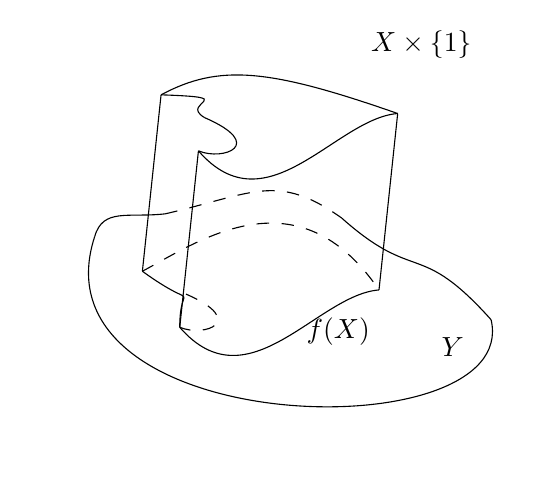
\begin{tikzpicture}[x=0.75pt,y=0.75pt,yscale=-1,xscale=1]
%uncomment if require: \path (0,333); %set diagram left start at 0, and has height of 333

%Curve Lines [id:da6444277677637305] 
\draw  [dash pattern={on 4.5pt off 4.5pt}]  (111.11,138.49) .. controls (139.11,123.49) and (186.11,90.49) .. (225.11,147.49) ;
%Curve Lines [id:da15933269378180293] 
\draw    (225.11,147.49) .. controls (195.22,149.83) and (162.11,203.49) .. (129.11,165.49) ;
%Straight Lines [id:da8713805055011097] 
\draw    (129.11,165.49) -- (138.11,80.49) ;
%Straight Lines [id:da5739490745379057] 
\draw    (234.11,62.49) -- (225.11,147.49) ;
%Straight Lines [id:da9424186414524165] 
\draw    (111.11,138.49) -- (120.11,53.49) ;
%Curve Lines [id:da06020756766297719] 
\draw    (111.11,138.49) .. controls (140.11,159.49) and (129.11,140.83) .. (129.11,165.49) ;
%Curve Lines [id:da6518113912028751] 
\draw  [dash pattern={on 4.5pt off 4.5pt}]  (132.11,149.49) .. controls (162.11,162.49) and (141.11,170.49) .. (129.11,165.49) ;
%Curve Lines [id:da6919048847206088] 
\draw    (88.11,121.83) .. controls (56.11,219.83) and (294.11,225.83) .. (279.11,161.83) ;
%Curve Lines [id:da26356149519388294] 
\draw    (88.11,121.83) .. controls (92.11,107.83) and (104.11,112.83) .. (122.11,110.83) ;
%Curve Lines [id:da925633666277923] 
\draw    (207.11,112.83) .. controls (243.11,144.83) and (244.11,122.83) .. (279.11,161.83) ;
%Curve Lines [id:da22227873309902302] 
\draw  [dash pattern={on 4.5pt off 4.5pt}]  (122.11,110.83) .. controls (165.11,100.83) and (176.11,90.83) .. (207.11,112.83) ;
%Curve Lines [id:da8795080597135727] 
\draw    (120.11,53.49) .. controls (148.11,38.49) and (172.11,40.83) .. (234.11,62.49) ;
%Curve Lines [id:da579791330936277] 
\draw    (234.11,62.49) .. controls (204.22,64.83) and (171.11,118.49) .. (138.11,80.49) ;
%Curve Lines [id:da623836388334464] 
\draw    (141.11,64.49) .. controls (171.11,77.49) and (150.11,85.49) .. (138.11,80.49) ;
%Curve Lines [id:da23519896120640116] 
\draw    (120.11,53.49) .. controls (160.11,54.83) and (128.11,56.83) .. (141.11,64.49) ;

% Text Node
\draw (189,159.4) node [anchor=north west][inner sep=0.75pt]    {$f( X)$};
% Text Node
\draw (220,21.4) node [anchor=north west][inner sep=0.75pt]    {$X\times \{1\}$};
% Text Node
\draw (254,169.4) node [anchor=north west][inner sep=0.75pt]    {$Y$};
\end{tikzpicture}\]
不难发现映射柱对于$X$也有一个嵌入映射$\iota_X : X \hookrightarrow Y \cup_f X \times I$.使得图表交换
\[\begin{tikzcd}
	X && Y \\
	\\
	&& {Y \cup_f X\times I}
	\arrow["f", from=1-1, to=1-3]
	\arrow["{\iota_Y}", from=1-3, to=3-3]
	\arrow["{\simeq \iota_X}"', from=1-1, to=3-3]
\end{tikzcd}\]
因此可以得到映射柱的一个作用:把任何映射都转变为一个嵌入映射.
\end{example}
为了配合理解,再增添两个例子配合消化.
\begin{example}
    $Y = S^1 \lor S^1$为$S^1$的一点和,将其两个圆分别记为$a$与$b$.
    接着考虑$D^2 \cong I \times I$,将其两条边分别记为$a$和$b$.接着,将$I \times I$上的$a$边粘在圆$a$上,将$I \times I$上的$b$边粘在圆$b$上.
    即
    \[\tikzset{every picture/.style={line width=0.75pt}} %set default line width to 0.75pt        
\begin{tikzpicture}[x=0.75pt,y=0.75pt,yscale=-1,xscale=1]
%uncomment if require: \path (0,349); %set diagram left start at 0, and has height of 349

%Shape: Ellipse [id:dp4483406660396818] 
\draw   (298.65,123.98) .. controls (298.39,117.01) and (299.53,111.39) .. (301.19,111.42) .. controls (302.85,111.45) and (304.4,117.13) .. (304.65,124.1) .. controls (304.9,131.07) and (303.77,136.69) .. (302.11,136.66) .. controls (300.45,136.62) and (298.9,130.95) .. (298.65,123.98) -- cycle ;
%Shape: Ellipse [id:dp9023826857993218] 
\draw   (285,103.36) .. controls (285,98.58) and (300.67,94.72) .. (320,94.72) .. controls (339.33,94.72) and (355,98.58) .. (355,103.36) .. controls (355,108.13) and (339.33,112) .. (320,112) .. controls (300.67,112) and (285,108.13) .. (285,103.36) -- cycle ;
\draw   (301.23,121.5) -- (300.01,134.9) -- (293.71,123.01) ;
\draw   (322,104.94) -- (337,110.97) -- (322,117) ;
%Straight Lines [id:da47795291834905806] 
\draw    (108.11,72.49) -- (185.11,72.49) ;
\draw [shift={(152.61,72.49)}, rotate = 180] [color={rgb, 255:red, 0; green, 0; blue, 0 }  ][line width=0.75]    (10.93,-3.29) .. controls (6.95,-1.4) and (3.31,-0.3) .. (0,0) .. controls (3.31,0.3) and (6.95,1.4) .. (10.93,3.29)   ;
%Straight Lines [id:da026838549565143532] 
\draw    (108.11,146.6) -- (185.11,146.6) ;
\draw [shift={(152.61,146.6)}, rotate = 180] [color={rgb, 255:red, 0; green, 0; blue, 0 }  ][line width=0.75]    (10.93,-3.29) .. controls (6.95,-1.4) and (3.31,-0.3) .. (0,0) .. controls (3.31,0.3) and (6.95,1.4) .. (10.93,3.29)   ;
%Straight Lines [id:da6097825619498349] 
\draw    (108.11,146.6) -- (108.11,72.49) ;
\draw [shift={(108.11,103.55)}, rotate = 90] [color={rgb, 255:red, 0; green, 0; blue, 0 }  ][line width=0.75]    (10.93,-3.29) .. controls (6.95,-1.4) and (3.31,-0.3) .. (0,0) .. controls (3.31,0.3) and (6.95,1.4) .. (10.93,3.29)   ;
%Straight Lines [id:da8720941867314604] 
\draw    (185.11,146.6) -- (185.11,72.49) ;
\draw [shift={(185.11,103.55)}, rotate = 90] [color={rgb, 255:red, 0; green, 0; blue, 0 }  ][line width=0.75]    (10.93,-3.29) .. controls (6.95,-1.4) and (3.31,-0.3) .. (0,0) .. controls (3.31,0.3) and (6.95,1.4) .. (10.93,3.29)   ;

% Text Node
\draw (349,79.4) node [anchor=north west][inner sep=0.75pt]    {$a$};
% Text Node
\draw (308,121.4) node [anchor=north west][inner sep=0.75pt]    {$b$};
% Text Node
\draw (140,154.4) node [anchor=north west][inner sep=0.75pt]    {$a$};
% Text Node
\draw (190,100.4) node [anchor=north west][inner sep=0.75pt]    {$b$};
% Text Node
\draw (142,48.4) node [anchor=north west][inner sep=0.75pt]    {$a^{-1}$};
% Text Node
\draw (75,102.4) node [anchor=north west][inner sep=0.75pt]    {$b^{-1}$};
\end{tikzpicture}\]
此时$I \times I$中$a$的对边也站到圆$a$上,但是$a$的对边的方向与绕$ab$所代表的箭头构成的方向相反,因此将其记为$a^{-1}$同理得到$b^{-1}$.最终我们得到的仍然是一个环面.因此可以得到$T \cong S^1 \lor S^1 \cup_{aba^{-1}b^{-1}}D^2$.
\end{example}
还有一些粘接是在三维空间中无法表示出来的
\begin{example}
    令$Y = S^1$,$D^2 = \{(x,y):x^2+y^2 = 4\}$.
    

    接下来我们打算将$D^2$以$1:1$的比例粘在$S^1$上(相当于绕了$S^1$两周)


    这样就得到了$S^1 \cup_2 D^2$不难发现其同胚于$\mathbb{R}P^2$.


    这个空间也就是常说的Moore空间.
\end{example}
\subsection{锥体的性质}
\begin{property}
    锥体的顶点是它的强形变收缩核,从而锥体是可缩的.
\end{property}
\begin{proof}
    映射$r : CX \to X \times \{1\}$是收缩映射.定义映射$H : CX \times I \to CX$,
    $$
    H((x,s),t) = (x,1-t+ts)
    $$
    不难发现$H$是连续的,且不难知道$\iota \circ r \simeq^H \text{id}_{CX}$,将$s = 1$带入上式,得到$H(v,t) = v$对于任意的$t \in I$成立.因此锥形$CX$的顶点是其强形变收缩核.
\end{proof}
显然,$x \in X$与$(x,0) \in CX$等同,$X$可以看成锥形$CX$的子集$X \times \{0\}$,$X$也是$CX$的一个子拓扑空间.对于映射$f : X \to Y$,如果存在映射$\overline{f} : CX \to Y$,使得$\overline{f}((x,0)) = f(x)$对于任意的$x \in X$成立,我们称映射$f$可以扩张到$CX$上,映射$\overline{f}$是映射$f$的扩张.
\begin{property}
    映射$f : X \to Y$同伦于一个常值映射当且仅当$f$可以扩张到锥形$CX$上.
\end{property}
\begin{proof}
    必要性: 设$y_0 \in Y$,同样以$y_0$表示从$X$到$Y$的常值映射,$y_0(x) = y_0$.如果有映射$F : X \times I \to Y$使得$f \simeq^F y_0 : X\to Y$.由于$F(x,1) = y_0$因此可以得到映射$F$诱导
    $$
    \tilde{F} : CX \to Y , \tilde{F}((x,t)) = F(x,t)
    $$
    显然有$\tilde{F}((x,0)) = F(x,0) = f(x)$因此称$\tilde{F}$是$f$在$CX$上的扩张.\\
    充分性: 设$\tilde{f}$是$f : X \to Y$的一个扩张,记$F  = \tilde{f} \circ \pi : X \times I \to Y$.即$F(x,t) = \tilde{f} (x,t)$,由于$F$是两个连续映射的复合,因此$F$也是连续的.记$y_1 = \tilde{f}(v)$,则$F(x,1) = y_1$,而$F(x,0) = f(x)$即$f(x) \simeq y_1$.
\end{proof}
\begin{corollary}
    映射$f:S^n \to Y$是零伦的充要条件是它可以被扩张到单位球体$D^{n+1}$上.
\end{corollary}
\begin{proof}
    如果$f$是零伦的,因此其同伦于一个常值映射,因此其可以被扩张到锥形$CS^n$上,由于$CS^n \cong D^{n+1}$因此其可以被扩张到$D^{n+1}$上.\\
    反之将$D^{n+1}$同胚到$CS^n$上,由于$f$可以被扩张到$CS^n$上,因此其是零伦.
\end{proof}
\subsection{习题}
习题节选自\cite{周建伟2007代数拓扑讲义}.
\begin{exercise}
设$f,g$都是常值映射,证明$f \simeq g$当且仅当$f(X)$,$g(X)$在$Y$的同一道路连通分支内.(此题建议在看完基本群中关于道路的定义后回顾)
\end{exercise}
\begin{solution}
    ($\Rightarrow$)若$f \simeq g$,则存在$F : X \times I \to Y$使得$F(x,0) = f(x)$且$F(x,1) = g(x)$.
    而由于$f$与$g$均为常值映射,因此有$f(x) = x_1 \in Y,g(x) = x_2 \in Y,\forall x \in X$.
    因此对于$F(x,t)$有$F(x,0) = x_1$且$F(x,1) = x_2$.因此$\sigma(t) = F(x,t)$是$Y$上的一个以$x_1$为起始点,$x_2$为终点的连续映射,因此$\sigma(t)$是一条道路.


    从而得到$x_1$与$x_2$处于$Y$的同一个道路连通分支内.即$f(X)$与$g(X)$处于$Y$的同一个道路连通分支内.\\
    ($\Leftarrow$)由于$f(X)$与$g(X)$处于$Y$的同一个道路连通分支内,因此可以找到一条道路$\sigma(t)$以$f(x)$为起点且以$g(x)$为终点($f(x)$与$g(x)$均为常值映射,因此$\sigma$存在).构建$F(x,t) = \sigma(t)$即可.不难发现$F(x,t)$是$f$与$g$的一个伦移.因此$f \simeq g$.
\end{solution}
\begin{exercise}
    设$f: S^1 \to S^1$为对径映射($f(x) = -x,\forall x\in S^1$),证明$f \simeq 1_{S^1}$.
\end{exercise}
\begin{solution}
    构建伦移$F : S^1 \times I \to S^1$使得$F(x,0) = -x$而$F(x,1) = x$即可.直接构建是有难度的,因此可以采用一些取巧的方式,将$S^1$使用极坐标进行表示$(1,\theta)$,有$f((1,\theta)) = (1,\theta+\pi)$.


    那么$F((1,\theta),t) = (1,\theta+(1-t)\pi)$此时有$F((1,\theta),0) = f((1,\theta))$且$F((1,\theta),1) = (1,\theta)$因此$f \simeq 1_S$.
\end{solution}
\begin{exercise}
    证明:$X$是可缩的拓扑空间当且仅当对任一拓扑空间$Z$以及任意两个映射$f,g : Z \to X$它们都同伦.由此证明可缩空间一定是道路连通的.
\end{exercise}
\begin{solution}
    ($\Rightarrow$)若$X$为一个可缩空间,则$X$同伦等价于一个独点空间$\{x_0\}$.因此$\{x_0\}$为$X$的一个形变收缩核.即对于$\iota : \{x_0\} \to X$,$\iota\circ c_{x_0} \simeq \text{id}_X$.


    考虑$f ,g :Z\to X$,有$\text{id}_X \circ f = f$且$\text{id}_X \circ g = g$.从而可以得到$\text{id}_X\circ f \simeq \iota\circ c_{x_0} \circ f$而$\iota \circ c_{x_0} \circ f(z) = x_0 = \iota \circ c_{x_0} \circ g(z)$
    因此有$\iota \circ c_{x_0} \circ f = \iota \circ c_{x_0} \circ g$又因为同伦关系是一个等价关系所以得到$f \simeq g$\\
    ($\Leftarrow$)若对于任意两个映射$f ,g : Z \to X$都有$f \simeq g$.因此考虑$\{x_0\} \to X$的所有映射(即$f$将$x_0$映射到任意一点)以及嵌入映射$\iota$.
    得到总是存在一个$\sigma(t): X\to X$使得对于任意的$x$都有$\sigma_x(0) = x$而$\sigma_x(1) = x_0$.
    因此考虑$F : X \times I \to X$,$F(x,t) = \sigma_x(t)$


    根据($\Leftarrow$)可以得知可收缩空间一定是道路连通的
\end{solution}
\begin{exercise}
    证明: 如果$f_i \simeq g_i: X_i \to Y_i,i= 1,2$,则$f_1 \times f_2 \simeq g_1 \times g_2: X_1 \times X_2  \to Y_1 \times Y_2$
\end{exercise}
\begin{solution}
    由于$f_i \simeq g_i$因此存在$F_i: X_i \times I \to Y_i$作为$f_i$与$g_i$的伦移.


    接下来考虑$F : X_1 \times X_2 \times I \to Y_1 \times Y_2$
    使得
    $$
    F((x_1,x_2),t) = (F(x_1,t),F(x_2,t))
    $$
    即可\\
    不难发现$F$是连续的并且$F((x_1,x_2),0) = (f_1(x_1),f_2(x_2))$,$F((x_1,x_2),1) = (g_1(x_1),g_2(x_2))$即$f_1 \times f_2 \simeq g_1 \times g_2$
\end{solution}
\begin{exercise}
    如果空间$X_i \simeq Y_i,i= 1,2$则$X_1 \times X_2 \simeq Y_1 \times Y_2$.
\end{exercise}
\begin{solution}
    若$X_i \simeq Y_i$则存在$f_i : X_i \to Y_i$以及$g_i : Y_i \to X_i$使得$f_i \circ g_i \simeq 1_{Y_i}$且$g_i \circ f_i \simeq 1_{X_i}$.


    因此存在$F_i : X_i \times I \to X_i$以及$G_i: Y_i \times I \to Y_i$使得$F_i(x,0) = g_i\circ f_i(x),F_i(x,1) = 1_{X_i}$且$G_i(x,0) = f_i \circ g_i (x),G_i(x,1) = g_i\circ f_i (x)$.
    
    
    令$F : X_1 \times X_2 \times I \to X_1 \times X_2$使得$F((x_1,x_2),t) = (F_i(x_1,t),F_i(x_2,t))$同理定义$G : Y_1 \times Y_2 \times I \to Y_1 \times Y_2$.

    有$F((x_1,x_2),0) = (g_1 \circ f_1(x_1),g_2 \circ f_2(x_2)) = g_1 \circ f_1 \times g_2 \circ f_2(x_1,x_2)$且$F((x_1,x_2),1) = 1_{X_1 \times X_2}$.因此$g_1 \circ f_1 \times g_2 \circ f_2 \simeq 1_{X_1 \times X_2}$.
    
    
    同理得到$G$的情况,因此有$X_1 \times X_2 \simeq Y_1 \times Y_2$.
\end{solution}
\begin{exercise}
    设$f : X \to Y$是同伦等价,则$f$的所有同伦逆彼此同伦.
\end{exercise}
\begin{solution}
    设$g_1,g_2$均为$f$的同伦逆,因此有$g_1 \circ f \simeq \text{id}_X \simeq g_2 \circ f$.且$f \circ g_1 \simeq \text{id}_Y \simeq f \circ g_2$.


    因此$g_1 \circ f \simeq g_2 \circ f$且$f \circ g_1 \simeq f \circ g_2$.得到$g_1 \circ f \circ g_1 \simeq g_1\circ f \circ g_2$而$g_1 \circ f \simeq \text{id}_X$这也就得到$g_1 \simeq g_2$.
\end{solution}
\begin{exercise}
    如果$f:X\to Y$,$g : Y\to Z$,$h : Z\to W$都是连续映射,使得$g \circ f : X \simeq Z$与$h \circ g : Y \simeq W$,证明,$f,g,h$都是同伦等价.
\end{exercise}
\begin{solution}
    由题意知,存在$k : Z \to X$使得$k \circ (g \circ f) \simeq \text{id}_X$且$(g \circ f) \circ k \simeq 1_Z$,由于$k \circ (g \circ f) = (k\circ g)\circ f \simeq \text{id}_X$.因此假设$k \circ g$是$f$的一个同伦逆.
    
    
    因此只需要证明$f \circ (k \circ g) \simeq \text{id}_Y$.


    由于$h \circ g: Y \simeq W$因此存在$k' : W \to Y$使得$k' \circ (h \circ g) \simeq \text{id}_Y$.


    观察到$h \circ g = h \circ 1_Z \circ g \simeq h \circ (g \circ f \circ k) \circ g = h \circ g \circ f \circ k \circ g$因此可以得出$f \circ k \circ g \simeq \text{id}_Y$.


    因此得到$k \circ g$就是$f$的同伦逆.即$f: X\simeq Y$.


    同理推知$g$和$h$都为同伦等价.
\end{solution}
\begin{exercise}
    证明可收缩空间的收缩核还是可收缩的.
\end{exercise}
\begin{solution}
    设$X$为一个可收缩空间,因此$X \simeq \{x_0\}$,即$\text{id}_X\simeq c_{x_0}$.


    考虑$X$的收缩核$A$,设$A$的嵌入映射为$\iota_A$,由于$A$是$X$的收缩核,因此存在$r : X \to A$使得$r \circ \iota_A = \text{id}_A$.不难发现$\text{id}_X$就是这样的一个$r$,由于$\text{id}_X \simeq c_{x_0}$因此$\text{id}_A \simeq c_{x_0}\circ \iota_A$.


    接下来考虑$c_{x_0}\circ \iota_A$得到$c_{x_0} \circ \iota_A (a) = x_0$.因此$c_{x_0} \circ \iota_A$是$A$上的常值映射.


    即$\text{id}_A \simeq c_{x_0}\mid_A$.因此$A$也是可收缩的.
\end{solution}
\begin{exercise}
    设$S_1,S_2$是平面上的两个不相交的圆,证明$S_1$是拓扑空间$X = S_1 \cup S_2$的收缩核,但不是形变收缩核.
\end{exercise}
\begin{solution}
    显然有$\text{id}_X \circ \iota_{S_1} = 1_{S_1}$因此$S_1$是$X$的一个收缩核.


    而$\iota_{S_1}\circ r(X)\subset S_1$.且$S_1 \cap S_2 = \varnothing$因此$\iota_{S_1} \circ r(X)$无法通过连续的变化变为$X$,从而$S_1$不是形变收缩核.
\end{solution}
\newpage
\section{基本群}
\subsection{引例}
对于$\frac{y}{x^2+y^2}$以及$\frac{x}{x^2+y^2}$在$\mathbb{R}^2 \setminus\{0\}$上连续,考虑曲线积分
$$
\int_{\gamma} -\frac{y}{x^2+y^2}\text{d}x + \frac{x}{x^2+y^2}\text{d}y
$$
令$P(x,y) = -\frac{y}{x^2+y^2}$,$Q(x,y) = \frac{x}{x^2+y^2}$.


由于
$$
\frac{\partial P}{\partial y} = -\frac{y^2-x^2}{(x^2+y^2)^2}\\
\frac{\partial Q}{\partial x} = -\frac{y^2-x^2}{(x^2+y^2)^2}
$$
因而曲线积分$\int_\gamma -\frac{y}{x^2+y^2}\text{d}x + \frac{x}{x^2+y^2}\text{d}y$与路径无关.


但是由于两者在原点$(0,0)$处均无定义.


考虑从$(x_1,y_1)$到$(x_2,y_2)$的三条曲线$\gamma_1,\gamma_2,\gamma_3$,如下图所示
\[\tikzset{every picture/.style={line width=0.75pt}} %set default line width to 0.75pt        
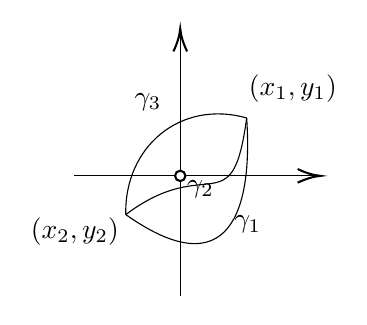
\begin{tikzpicture}[x=0.75pt,y=0.75pt,yscale=-1,xscale=1]
%uncomment if require: \path (0,300); %set diagram left start at 0, and has height of 300

%Curve Lines [id:da06870559142377042] 
\draw    (71,129) .. controls (121.24,164.45) and (132.24,126.45) .. (129.24,82.45) ;
%Curve Lines [id:da03251989569283409] 
\draw    (71,129) .. controls (111,99) and (122.24,134.45) .. (129.24,82.45) ;
%Curve Lines [id:da42661252124249494] 
\draw    (71,129) .. controls (70.24,96.45) and (97.24,73.45) .. (129.24,82.45) ;
%Shape: Circle [id:dp23193182681150648] 
\draw  [line width=0.75]  (94.74,110.35) .. controls (94.74,108.97) and (95.86,107.85) .. (97.24,107.85) .. controls (98.62,107.85) and (99.74,108.97) .. (99.74,110.35) .. controls (99.74,111.73) and (98.62,112.85) .. (97.24,112.85) .. controls (95.86,112.85) and (94.74,111.73) .. (94.74,110.35) -- cycle ;
%Straight Lines [id:da7506863408517561] 
\draw    (99.74,110.35) -- (162.74,110.35) ;
\draw [shift={(164.74,110.35)}, rotate = 180] [color={rgb, 255:red, 0; green, 0; blue, 0 }  ][line width=0.75]    (10.93,-3.29) .. controls (6.95,-1.4) and (3.31,-0.3) .. (0,0) .. controls (3.31,0.3) and (6.95,1.4) .. (10.93,3.29)   ;
%Straight Lines [id:da4964285997124258] 
\draw    (46.24,110.35) -- (94.74,110.35) ;
%Straight Lines [id:da4909197855746936] 
\draw    (97.24,107.85) -- (97.24,41.45) ;
\draw [shift={(97.24,39.45)}, rotate = 90] [color={rgb, 255:red, 0; green, 0; blue, 0 }  ][line width=0.75]    (10.93,-3.29) .. controls (6.95,-1.4) and (3.31,-0.3) .. (0,0) .. controls (3.31,0.3) and (6.95,1.4) .. (10.93,3.29)   ;
%Straight Lines [id:da674675323101249] 
\draw    (97.24,112.85) -- (97.24,168.45) ;

% Text Node
\draw (129,60.4) node [anchor=north west][inner sep=0.75pt]    {$(x_{1} ,y_{1})$};
% Text Node
\draw (24,129.4) node [anchor=north west][inner sep=0.75pt]    {$( x_{2} ,y_{2})$};
% Text Node
\draw (122,128.4) node [anchor=north west][inner sep=0.75pt]    {$\gamma _{1}$};
% Text Node
\draw (99.24,111.25) node [anchor=north west][inner sep=0.75pt]    {$\gamma _{2}$};
% Text Node
\draw (74,69.4) node [anchor=north west][inner sep=0.75pt]    {$\gamma _{3}$};


\end{tikzpicture}\]
首先考虑$\gamma_1$与$\gamma_2$的情况,由于$\gamma_1$与$\gamma_2$所围区域不包含原点,因此.
$$
\int_{\gamma_1} -\frac{y}{x^2+y^2}\text{d}x + \frac{x}{x^2+y^2}\text{d}y = \int_{\gamma_2} -\frac{y}{x^2+y^2}\text{d}x + \frac{x}{x^2+y^2}\text{d}y
$$
这是因为$\gamma_1$与$\gamma_2$所围成的闭区域$D$不包含原点,使用Green公式得到
$$
\oint_{\gamma_1 \cup \gamma_2} (P(x,y)\text{d}x+ Q(x,y)\text{d}y) = \iint_{D}(\frac{\partial Q}{\partial x} - \frac{\partial P}{\partial y}) \text{d}x\text{d}y= 0
$$
接下来考虑$\gamma_2$与$\gamma_3$所围成的封闭区域,这个封闭区域包含原点,因此
$$
\int_{\gamma_2} -\frac{y}{x^2+y^2}\text{d}x + \frac{x}{x^2+y^2}\text{d}y \neq\int_{\gamma_3} -\frac{y}{x^2+y^2}\text{d}x + \frac{x}{x^2+y^2}\text{d}y
$$
这是为什么呢?


由前文知该积分与路径无关,并且$\gamma_2$与$\gamma_3$所围的闭曲线只绕原点转了一圈,因此它等价于一个绕原点一圈的圆.
\[\tikzset{every picture/.style={line width=0.75pt}} %set default line width to 0.75pt        
\begin{tikzpicture}[x=0.75pt,y=0.75pt,yscale=-1,xscale=1]
%uncomment if require: \path (0,300); %set diagram left start at 0, and has height of 300

%Straight Lines [id:da8967222639034556] 
\draw    (119.74,130.35) -- (182.74,130.35) ;
\draw [shift={(184.74,130.35)}, rotate = 180] [color={rgb, 255:red, 0; green, 0; blue, 0 }  ][line width=0.75]    (10.93,-3.29) .. controls (6.95,-1.4) and (3.31,-0.3) .. (0,0) .. controls (3.31,0.3) and (6.95,1.4) .. (10.93,3.29)   ;
%Straight Lines [id:da6121366738703817] 
\draw    (66.24,130.35) -- (114.74,130.35) ;
%Straight Lines [id:da7441230748182697] 
\draw    (117.24,127.85) -- (117.24,61.45) ;
\draw [shift={(117.24,59.45)}, rotate = 90] [color={rgb, 255:red, 0; green, 0; blue, 0 }  ][line width=0.75]    (10.93,-3.29) .. controls (6.95,-1.4) and (3.31,-0.3) .. (0,0) .. controls (3.31,0.3) and (6.95,1.4) .. (10.93,3.29)   ;
%Straight Lines [id:da1010791338820205] 
\draw    (117.24,132.85) -- (117.24,188.45) ;
%Shape: Circle [id:dp3303446961731127] 
\draw  [line width=0.75]  (114.74,130.35) .. controls (114.74,128.97) and (115.86,127.85) .. (117.24,127.85) .. controls (118.62,127.85) and (119.74,128.97) .. (119.74,130.35) .. controls (119.74,131.73) and (118.62,132.85) .. (117.24,132.85) .. controls (115.86,132.85) and (114.74,131.73) .. (114.74,130.35) -- cycle ;
%Shape: Circle [id:dp37478675775873693] 
\draw   (92.24,130.35) .. controls (92.24,116.54) and (103.43,105.35) .. (117.24,105.35) .. controls (131.05,105.35) and (142.24,116.54) .. (142.24,130.35) .. controls (142.24,144.16) and (131.05,155.35) .. (117.24,155.35) .. controls (103.43,155.35) and (92.24,144.16) .. (92.24,130.35) -- cycle ;
\draw   (116.89,149.36) .. controls (122.67,151.13) and (127.86,151.48) .. (132.47,150.41) .. controls (128.45,152.9) and (125.02,156.82) .. (122.18,162.15) ;

% Text Node
\draw (140,146.4) node [anchor=north west][inner sep=0.75pt]    {$\gamma $};


\end{tikzpicture}\]

接下来取$\mathbb{R}^2 \setminus\{(0,0)\}$的一条曲线$\gamma$
$$
\gamma = \left\{
\begin{array}{c}
x = \cos \theta \\
y = \sin \theta \\
\end{array},
0 \leq \theta \leq 2\pi
\right.
$$
得到
\begin{eqnarray*}
    \oint_{\gamma} -\frac{y}{x^2+y^2}\text{d}x + \frac{x}{x^2+y^2}\text{d}y &=& \int_{0}^{2\pi} -\frac{\sin \theta}{1}(-\sin \theta)\text{d}\theta + \frac{\cos \theta}{1}(\cos \theta)\text{d}\theta 
    \\ 
    &=& \int_{0}^{2\pi} \text{d}\theta = 2\pi 
\end{eqnarray*}

而$\int_{\gamma_3 \cup \gamma_2} \cdot = \int_\gamma\cdot$因此得到二者不相等.


此外,还可以进行推广,对于任何$\mathbb{R}^2 \setminus\{(0,0)\}$中的闭曲线$\gamma$有
$$
\oint_{\gamma} -\frac{y}{x^2+y^2}\text{d}x + \frac{x}{x^2+y^2}\text{d}y = 2k\pi(k \in \mathbb{Z})
$$
其中$k$表示闭曲线绕原点正向(逆时针)旋转的周数.


由于$k$与具体的形状无关,因此$k$也是一个拓扑性质,$\mathbb{Z}$就是$\mathbb{R}^2 \setminus\{(0,0)\}$的一个基本群.
\subsection{道路同伦}
在开始之前,先问一个问题,什么是道路?在数学中又该如何定义它?


在生活中,道路就是供我们通行的路径(比如高速公路就是道路的一种),有起点也有终点.在日常出行中,我们走的路也是有起点也有终点的,并且总是能够在经过一段时间后到达终点上.


接下来,将日常生活的空间视为一个拓扑空间,把自己视为拓扑空间中的一个点,在日常出行中,从出发位置到目的地,就是一个点到另一个点的移动过程.


而道路,就是连接这两点的一条线(不一定是直线),由于总是能够在一段时间内到达目的地,因此从起始点出发到目的地的时间段可以视为一个$\mathbb{R}$上的闭区间,既然是一个闭区间,那就同胚于$I$(简单来说就是将出发时刻记为$0$,将到达时刻记为$1$)由于人在空间中是不会闪现的,因此行走的道路自然也是连续的.


因此道路可以抽象为一个连续的映射,以下是其具体定义.
\begin{definition}
    映射$\sigma : I \to X$在$\sigma(0) = x_0$,$\sigma(1) = x_1$时被称为$X$中从$x_0$到$x_1$的一条道路.对$X$中两条从$x_0$到$x_1$的道路$\sigma,\tau$如果存在伦移$F: I \times I \to X$使得$F(s,0) = \sigma(s)$,$F(s,1) = \tau(s)$且有$F(0,t) = x_0$且$F(1,t) = x_1$恒成立,则称$\sigma$与$\tau$道路同伦,称$F$为从$\sigma$到$\tau$的道路伦移,记为$\sigma\simeq_p^F\tau$或$\sigma\simeq_p \tau$.有时也简记为$\sigma \simeq \tau\quad \text{rel} \{0,1\}$
\end{definition}
\[\tikzset{every picture/.style={line width=0.75pt}} %set default line width to 0.75pt        
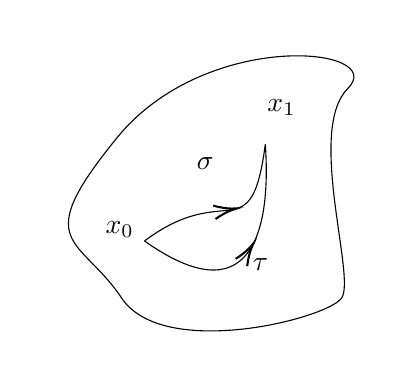
\begin{tikzpicture}[x=0.75pt,y=0.75pt,yscale=-1,xscale=1]
%uncomment if require: \path (0,300); %set diagram left start at 0, and has height of 300

%Curve Lines [id:da06870559142377042] 
\draw    (71,129) .. controls (121.24,164.45) and (132.24,126.45) .. (129.24,82.45) ;
\draw [shift={(123.54,130.12)}, rotate = 122.21] [color={rgb, 255:red, 0; green, 0; blue, 0 }  ][line width=0.75]    (10.93,-3.29) .. controls (6.95,-1.4) and (3.31,-0.3) .. (0,0) .. controls (3.31,0.3) and (6.95,1.4) .. (10.93,3.29)   ;
%Curve Lines [id:da03251989569283409] 
\draw    (71,129) .. controls (111,99) and (122.24,134.45) .. (129.24,82.45) ;
\draw [shift={(115.45,113.32)}, rotate = 170.17] [color={rgb, 255:red, 0; green, 0; blue, 0 }  ][line width=0.75]    (10.93,-3.29) .. controls (6.95,-1.4) and (3.31,-0.3) .. (0,0) .. controls (3.31,0.3) and (6.95,1.4) .. (10.93,3.29)   ;
%Shape: Polygon Curved [id:ds048370975326988086] 
\draw   (58,79) .. controls (101,26.49) and (189,35.49) .. (169,55.49) .. controls (149,75.49) and (173,146.49) .. (166,156.49) .. controls (159,166.49) and (80,186.49) .. (60,156.49) .. controls (40,126.49) and (15,131.51) .. (58,79) -- cycle ;

% Text Node
\draw (95,87.4) node [anchor=north west][inner sep=0.75pt]    {$\sigma $};
% Text Node
\draw (51,118.4) node [anchor=north west][inner sep=0.75pt]    {$x_{0}$};
% Text Node
\draw (129,59.4) node [anchor=north west][inner sep=0.75pt]    {$x_{1}$};
% Text Node
\draw (122,136.4) node [anchor=north west][inner sep=0.75pt]    {$\tau $};


\end{tikzpicture}\]
为什么道路同伦这个概念需要区别于同伦而单独提出来呢?我们通过一个例子来增进理解.
\begin{example}
    若$X$为一个道路连通空间,$\sigma,\tau : I \to X$为$X$上的任意两条道路,不妨设$\sigma(0) = x_0$且$\tau(0) =x_0'$.
    \[\tikzset{every picture/.style={line width=0.75pt}} %set default line width to 0.75pt       
    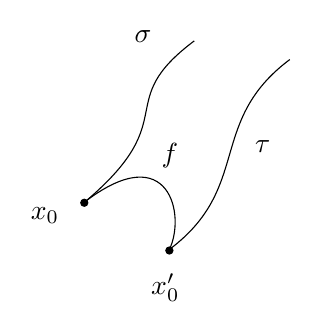
\begin{tikzpicture}[x=0.75pt,y=0.75pt,yscale=-1,xscale=1]
    %uncomment if require: \path (0,300); %set diagram left start at 0, and has height of 300
    
    %Shape: Free Drawing [id:dp5082817438840954] 
    \draw  [line width=3] [line join = round][line cap = round] (258,202.49) .. controls (258,202.49) and (258,202.49) .. (258,202.49) ;
    %Shape: Free Drawing [id:dp3307765313110329] 
    \draw  [line width=3] [line join = round][line cap = round] (299,225.49) .. controls (299,225.49) and (299,225.49) .. (299,225.49) ;
    %Curve Lines [id:da7696510424591116] 
    \draw    (259,201.49) .. controls (306,161.49) and (271,154.49) .. (311,124.49) ;
    %Curve Lines [id:da26510510560661493] 
    \draw    (299,225) .. controls (339,195) and (317,163.49) .. (357,133.49) ;
    %Curve Lines [id:da22288900476686457] 
    \draw    (259,201.49) .. controls (299,171.49) and (307,208.49) .. (299,225) ;
    
    % Text Node
    \draw (231,203.4) node [anchor=north west][inner sep=0.75pt]    {$x_{0}$};
    % Text Node
    \draw (281,118.4) node [anchor=north west][inner sep=0.75pt]    {$\sigma $};
    % Text Node
    \draw (339,171.4) node [anchor=north west][inner sep=0.75pt]    {$\tau $};
    % Text Node
    \draw (289,235.4) node [anchor=north west][inner sep=0.75pt]    {$x_{0} '$};
    % Text Node
    \draw (294,172.4) node [anchor=north west][inner sep=0.75pt]    {$f$};
    \end{tikzpicture}\]    
   选定一条从$x_0 \to x_0'$的道路$f$.
   不难看出存在以下映射.
   \begin{eqnarray*}
    F_1 : I \times I &\to& X\\
    F_1(s,t) &=& \sigma(s(1-t))\\
    F_1(s,0) &=& \sigma(s)\\
    F_1(s,1) &\equiv& \sigma(0) = x_0
   \end{eqnarray*}
   类似地,定义
   \begin{eqnarray*}
    F_2 : I \times I &\to& X\\
    F_2(s,t) &=& f(t)\\
    F_2(s,0) &\equiv & f(0) = x_0\\
    F_2(s,1) &\equiv & f(1) = x_0'
   \end{eqnarray*}
   以及
   \begin{eqnarray*}
    F_3 : I \times I &\to& X\\
    F_3(s,t) &=& \tau(st)\\
    F_3(s,0) &\equiv& \tau(0) = x_0'\\
    F_3(s,1) &=& \tau(s)
   \end{eqnarray*}
接下来使用配凑大法将$F_1,F_2,F_3$连在一起.令
$$
F(s,t) = \left\{
    \begin{array}{c}
        F_1(s,t) ,0 \leq t \leq 1/3\\
        F_2(s,3t-1) , 1/3 \leq t \leq 2/3\\
        F_3(s,3t-2) , 2/3 \leq t \leq 1
    \end{array}
\right.
$$
如此这般,就得到了一个$\sigma$到$\tau$的伦移,因此$\sigma \simeq \tau$.

所以,在一个道路连通分支内,任意两条道路都是同伦的,因此,为作区分,将道路同伦这一概念定义为起终点相同的道路.
\end{example}


\begin{example}
    $\mathbb{R}^n$中从$x_0$到$x_1$的任意两条道路都是道路同伦的.
\end{example}

不难发现,道路同伦也是一个等价关系.
\begin{proposition}
    $X$中所有从$x_0$到$x_1$的道路所构成的集合中道路同伦$\simeq_p$为一个等价关系
\end{proposition}
\begin{proof}
    略
\end{proof}
\begin{definition}
    将$X$中所有的道路记为$PX$,它是一个拓扑空间(有所谓的紧开拓扑).那么道路同伦等价类记为
    $$
    PX /\simeq_p  = \{[\sigma]:\sigma \text{是}X\text{中的道路}\}
    $$
\end{definition}

由于道路同伦是一个等价关系,因此可以在$PX$中赋予一种商结构,将$PX/\simeq_p$称为一个道路同伦商集.


接下来,选定$X$中一点$x_0$令$P_{(X,x_0)}$为所有从$x_0$出发的道路所构成的集合,即
$$
P_{(X,x_0)} := \{\sigma : I \to X : \sigma(0) = x_0\}
$$
自然地,对于道路的终点可以得到一个映射$\pi : P_{(X,x_0)}\to X$将$\sigma$映射到$\sigma(1)$上.


因此考虑其逆$\pi^{-1}(x_1)$得到
$$
\pi^{-1}(x_1) = \{\sigma : I \to X : \sigma(0) = x_0,\sigma(1) = x_1\}
$$

特别地,取$x_1 = x_0$时,有
$$
\pi^{-1}(x_0) = \{\sigma : I \to X : \sigma(0) = \sigma(1) = x_0\}
$$
将$pi^{-1}(x_0)$记作$\Omega X$,称为回路空间.


我们为什么要费那么大功夫去搞这个回路空间呢?
\subsection{道路的合成(道路乘积)与基本群定义}
现在我们有两条首尾相连的道路$\sigma,\tau$($\sigma(1) = \tau(0)$).打算像在命题\ref{Pro:2.2.2}将$F$与$G$连起来一般,将$\sigma$与$\tau$这两条道路连起来.
\[\tikzset{every picture/.style={line width=0.75pt}} %set default line width to 0.75pt        
\begin{tikzpicture}[x=0.75pt,y=0.75pt,yscale=-1,xscale=1]
%uncomment if require: \path (0,139); %set diagram left start at 0, and has height of 139

%Shape: Free Drawing [id:dp1843163846894187] 
\draw  [line width=3] [line join = round][line cap = round] (60.11,59.97) .. controls (60.11,59.97) and (60.11,59.97) .. (60.11,59.97) ;
%Shape: Free Drawing [id:dp5605149749067355] 
\draw  [line width=3] [line join = round][line cap = round] (152.11,90.97) .. controls (152.11,90.97) and (152.11,90.97) .. (152.11,90.97) ;
%Shape: Free Drawing [id:dp907744320416149] 
\draw  [line width=3] [line join = round][line cap = round] (242.11,39.97) .. controls (242.11,39.97) and (242.11,39.97) .. (242.11,39.97) ;
%Curve Lines [id:da6817533462288632] 
\draw    (60.11,59.97) .. controls (100.11,29.97) and (111.11,120.97) .. (151.11,90.97) ;
\draw [shift={(109.83,80.46)}, rotate = 229.78] [color={rgb, 255:red, 0; green, 0; blue, 0 }  ][line width=0.75]    (10.93,-3.29) .. controls (6.95,-1.4) and (3.31,-0.3) .. (0,0) .. controls (3.31,0.3) and (6.95,1.4) .. (10.93,3.29)   ;
%Curve Lines [id:da7274614261760568] 
\draw    (151.11,90.97) .. controls (191.11,60.97) and (147.11,38.97) .. (241.11,39.97) ;
\draw [shift={(190.25,44.05)}, rotate = 159.15] [color={rgb, 255:red, 0; green, 0; blue, 0 }  ][line width=0.75]    (10.93,-3.29) .. controls (6.95,-1.4) and (3.31,-0.3) .. (0,0) .. controls (3.31,0.3) and (6.95,1.4) .. (10.93,3.29)   ;

% Text Node
\draw (35,31.73) node [anchor=north west][inner sep=0.75pt]    {$x_{0}$};
% Text Node
\draw (139,57.73) node [anchor=north west][inner sep=0.75pt]    {$x_{1}$};
% Text Node
\draw (244,13.73) node [anchor=north west][inner sep=0.75pt]    {$x_{2}$};
% Text Node
\draw (87,62.73) node [anchor=north west][inner sep=0.75pt]    {$\sigma $};
% Text Node
\draw (183,23.73) node [anchor=north west][inner sep=0.75pt]    {$\tau $};
\end{tikzpicture}\]
这就引出了定义
\begin{definition}
    设$\sigma,\tau: I\to X$为$X$中的两条道路,若$\sigma(1) = \tau(0)$(条件),则其道路的乘积$\sigma \cdot \tau$被定义为
    $$
    \sigma \cdot \tau (s) =\left\{
        \begin{array}{c}
            \sigma(2s) , 0\leq s \leq 1/2\\
            \tau(2s - 1), 1/2 \leq s \leq 1
        \end{array}
    \right.
    $$
\end{definition}
不难发现,不是所有的$\sigma ,\tau \in PX$都满足上述条件,因而先研究一个必然满足这一条件的集合,也就是前文构建的回路空间$\Omega X$.


可以发现道路乘积定义了一个运算
\begin{eqnarray*}
    \Omega X \times \Omega X &\to& \Omega X\\
    (\sigma,\tau) &\mapsto& \sigma \cdot \tau
\end{eqnarray*}
不难发现,道路的合成也是道路,既然是道路,那道路同伦关系就是一个等价关系,因此可以考虑对其进行分类(找到其等价类).
\begin{lemma}
    设$X$中的道路$\sigma \simeq_p \sigma'$,$\tau \simeq_p \tau'$如果$\sigma(1) = \tau(0)$则有$\sigma \cdot \tau \simeq_p \sigma' \cdot \tau'$.
    \[\tikzset{every picture/.style={line width=0.75pt}} %set default line width to 0.75pt        
    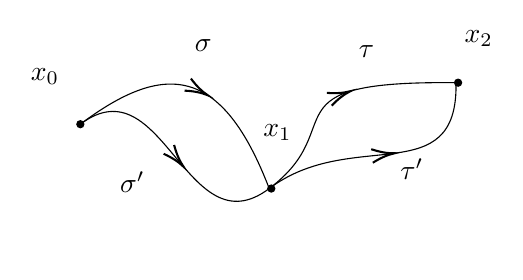
\begin{tikzpicture}[x=0.75pt,y=0.75pt,yscale=-1,xscale=1]
    %uncomment if require: \path (0,171); %set diagram left start at 0, and has height of 171
    
    %Shape: Free Drawing [id:dp1843163846894187] 
    \draw  [line width=3] [line join = round][line cap = round] (60.11,59.97) .. controls (60.11,59.97) and (60.11,59.97) .. (60.11,59.97) ;
    %Shape: Free Drawing [id:dp5605149749067355] 
    \draw  [line width=3] [line join = round][line cap = round] (152.11,90.97) .. controls (152.11,90.97) and (152.11,90.97) .. (152.11,90.97) ;
    %Shape: Free Drawing [id:dp907744320416149] 
    \draw  [line width=3] [line join = round][line cap = round] (242.11,39.97) .. controls (242.11,39.97) and (242.11,39.97) .. (242.11,39.97) ;
    %Curve Lines [id:da6817533462288632] 
    \draw    (60.11,59.97) .. controls (100.11,29.97) and (128.11,30.97) .. (151.11,90.97) ;
    \draw [shift={(121.5,46.03)}, rotate = 208.02] [color={rgb, 255:red, 0; green, 0; blue, 0 }  ][line width=0.75]    (10.93,-3.29) .. controls (6.95,-1.4) and (3.31,-0.3) .. (0,0) .. controls (3.31,0.3) and (6.95,1.4) .. (10.93,3.29)   ;
    %Curve Lines [id:da7274614261760568] 
    \draw    (151.11,90.97) .. controls (191.11,60.97) and (147.11,38.97) .. (241.11,39.97) ;
    \draw [shift={(190.25,44.05)}, rotate = 159.15] [color={rgb, 255:red, 0; green, 0; blue, 0 }  ][line width=0.75]    (10.93,-3.29) .. controls (6.95,-1.4) and (3.31,-0.3) .. (0,0) .. controls (3.31,0.3) and (6.95,1.4) .. (10.93,3.29)   ;
    %Curve Lines [id:da7875605958108474] 
    \draw    (60.11,59.97) .. controls (100.11,29.97) and (111.11,120.97) .. (151.11,90.97) ;
    \draw [shift={(109.83,80.46)}, rotate = 229.78] [color={rgb, 255:red, 0; green, 0; blue, 0 }  ][line width=0.75]    (10.93,-3.29) .. controls (6.95,-1.4) and (3.31,-0.3) .. (0,0) .. controls (3.31,0.3) and (6.95,1.4) .. (10.93,3.29)   ;
    %Curve Lines [id:da761050411421468] 
    \draw    (151.11,90.97) .. controls (191.11,60.97) and (242.11,92.63) .. (241.11,39.97) ;
    \draw [shift={(211.49,73.97)}, rotate = 173.16] [color={rgb, 255:red, 0; green, 0; blue, 0 }  ][line width=0.75]    (10.93,-3.29) .. controls (6.95,-1.4) and (3.31,-0.3) .. (0,0) .. controls (3.31,0.3) and (6.95,1.4) .. (10.93,3.29)   ;
    
    % Text Node
    \draw (35,31.73) node [anchor=north west][inner sep=0.75pt]    {$x_{0}$};
    % Text Node
    \draw (147,58.73) node [anchor=north west][inner sep=0.75pt]    {$x_{1}$};
    % Text Node
    \draw (244,13.73) node [anchor=north west][inner sep=0.75pt]    {$x_{2}$};
    % Text Node
    \draw (114,17.73) node [anchor=north west][inner sep=0.75pt]    {$\sigma $};
    % Text Node
    \draw (193,20.73) node [anchor=north west][inner sep=0.75pt]    {$\tau $};
    % Text Node
    \draw (78,81.4) node [anchor=north west][inner sep=0.75pt]    {$\sigma '$};
    % Text Node
    \draw (213,75.4) node [anchor=north west][inner sep=0.75pt]    {$\tau '$};

    \end{tikzpicture}\]
    \label{lem:2.3.1}
\end{lemma}
\begin{proof}
    设$F : I \times I \to X$是从$\sigma$到$\sigma'$的道路伦移,$G : I \times I \to X$是$\tau$到$\tau'$的道路伦移.
    \[\tikzset{every picture/.style={line width=0.75pt}} %set default line width to 0.75pt        
    \begin{tikzpicture}[x=0.75pt,y=0.75pt,yscale=-1,xscale=1]
    %uncomment if require: \path (0,240); %set diagram left start at 0, and has height of 240
    
    %Straight Lines [id:da1048989390886439] 
    \draw    (100,115) -- (100,33.97) ;
    \draw [shift={(100,31.97)}, rotate = 90] [color={rgb, 255:red, 0; green, 0; blue, 0 }  ][line width=0.75]    (10.93,-3.29) .. controls (6.95,-1.4) and (3.31,-0.3) .. (0,0) .. controls (3.31,0.3) and (6.95,1.4) .. (10.93,3.29)   ;
    %Straight Lines [id:da007610078873852011] 
    \draw    (100,115) -- (197.11,115) ;
    \draw [shift={(199.11,115)}, rotate = 180] [color={rgb, 255:red, 0; green, 0; blue, 0 }  ][line width=0.75]    (10.93,-3.29) .. controls (6.95,-1.4) and (3.31,-0.3) .. (0,0) .. controls (3.31,0.3) and (6.95,1.4) .. (10.93,3.29)   ;
    %Straight Lines [id:da07472037644264229] 
    \draw    (100,73.49) -- (152.11,73.49) ;
    %Straight Lines [id:da11204901187947547] 
    \draw    (152.11,73.49) -- (152.11,115) ;
    %Straight Lines [id:da04646677663877119] 
    \draw    (126.06,73.49) -- (126.06,114.97) ;
    
    % Text Node
    \draw (84,18.4) node [anchor=north west][inner sep=0.75pt]    {$t$};
    % Text Node
    \draw (201.11,118.4) node [anchor=north west][inner sep=0.75pt]    {$s$};
    % Text Node
    \draw (107,54.4) node [anchor=north west][inner sep=0.75pt]    {$\sigma '$};
    % Text Node
    \draw (135,54.4) node [anchor=north west][inner sep=0.75pt]    {$\tau '$};
    % Text Node
    \draw (109,117.4) node [anchor=north west][inner sep=0.75pt]    {$\sigma $};
    % Text Node
    \draw (135,118.4) node [anchor=north west][inner sep=0.75pt]    {$\tau $};
    % Text Node
    \draw (108,85.4) node [anchor=north west][inner sep=0.75pt]    {$F$};
    % Text Node
    \draw (133,85.4) node [anchor=north west][inner sep=0.75pt]    {$G$}; 
    \end{tikzpicture}\]    
    考虑$\sigma \cdot \tau$与$\sigma' \cdot \tau'$.
    \begin{eqnarray*}
        \sigma \cdot \tau(s) &=& \left\{
        \begin{array}{c}
        \sigma(2s), 0 \leq s \leq 1/2\\
        \tau(2s-1), 1/2 \leq s \leq 1\\
        \end{array}
        \right.\\
        \sigma' \cdot \tau'(s) &=& \left\{
        \begin{array}{c}
        \sigma'(2s), 0 \leq s \leq 1/2\\
        \tau'(2s-1), 1/2 \leq s \leq 1\\
        \end{array}
        \right.
    \end{eqnarray*}
    不难发现$\sigma$与$\sigma'$均分别在$\sigma \cdot \tau$与$\sigma' \cdot \tau'$的$[0,1/2]$段而$\tau$部分在$[1/2,1]$段.


    因此可以分别对于$s \in [0,1/2]$以及$s \in [1/2,1]$两个部分进行考虑,不难发现前半段将$\sigma$转变为$\sigma'$的方式无非就是$F$,而后半段就是$G$,因此可以构建
    $$
    H(s,t) = \left\{
\begin{array}{c}
    F(2s,t),0\leq s \leq 1/2\\
    G(2s-1,t),1/2 \leq s \leq 1\\
\end{array}
    \right.
    $$
    不难发现,$H$将$\sigma \cdot \tau$伦移为$\sigma' \cdot \tau'$.即其为$\sigma \cdot \tau$到$\sigma' \cdot \tau'$的道路伦移.
\end{proof}
接下来在$\sigma$与$\tau$以外给出一段道路$\omega$使得$\omega(0) = \tau(1)$,如图所示.
\[\tikzset{every picture/.style={line width=0.75pt}} %set default line width to 0.75pt        
\begin{tikzpicture}[x=0.75pt,y=0.75pt,yscale=-1,xscale=1]
%uncomment if require: \path (0,171); %set diagram left start at 0, and has height of 171

%Shape: Free Drawing [id:dp1843163846894187] 
\draw  [line width=3] [line join = round][line cap = round] (60.11,59.97) .. controls (60.11,59.97) and (60.11,59.97) .. (60.11,59.97) ;
%Shape: Free Drawing [id:dp5605149749067355] 
\draw  [line width=3] [line join = round][line cap = round] (152.11,90.97) .. controls (152.11,90.97) and (152.11,90.97) .. (152.11,90.97) ;
%Shape: Free Drawing [id:dp907744320416149] 
\draw  [line width=3] [line join = round][line cap = round] (242.11,39.97) .. controls (242.11,39.97) and (242.11,39.97) .. (242.11,39.97) ;
%Curve Lines [id:da6817533462288632] 
\draw    (60.11,59.97) .. controls (100.11,29.97) and (128.11,30.97) .. (151.11,90.97) ;
\draw [shift={(121.5,46.03)}, rotate = 208.02] [color={rgb, 255:red, 0; green, 0; blue, 0 }  ][line width=0.75]    (10.93,-3.29) .. controls (6.95,-1.4) and (3.31,-0.3) .. (0,0) .. controls (3.31,0.3) and (6.95,1.4) .. (10.93,3.29)   ;
%Curve Lines [id:da7274614261760568] 
\draw    (151.11,90.97) .. controls (191.11,60.97) and (147.11,38.97) .. (241.11,39.97) ;
\draw [shift={(190.25,44.05)}, rotate = 159.15] [color={rgb, 255:red, 0; green, 0; blue, 0 }  ][line width=0.75]    (10.93,-3.29) .. controls (6.95,-1.4) and (3.31,-0.3) .. (0,0) .. controls (3.31,0.3) and (6.95,1.4) .. (10.93,3.29)   ;
%Shape: Free Drawing [id:dp055216021293476025] 
\draw  [line width=3] [line join = round][line cap = round] (203.11,88.63) .. controls (203.11,88.63) and (203.11,88.63) .. (203.11,88.63) ;
%Curve Lines [id:da9036501942071511] 
\draw    (241.11,39.97) .. controls (281.11,9.97) and (210.11,151.63) .. (202.11,89.63) ;
\draw [shift={(234.88,84.48)}, rotate = 302.22] [color={rgb, 255:red, 0; green, 0; blue, 0 }  ][line width=0.75]    (10.93,-3.29) .. controls (6.95,-1.4) and (3.31,-0.3) .. (0,0) .. controls (3.31,0.3) and (6.95,1.4) .. (10.93,3.29)   ;

% Text Node
\draw (35,31.73) node [anchor=north west][inner sep=0.75pt]    {$x_{0}$};
% Text Node
\draw (147,58.73) node [anchor=north west][inner sep=0.75pt]    {$x_{1}$};
% Text Node
\draw (244,13.73) node [anchor=north west][inner sep=0.75pt]    {$x_{2}$};
% Text Node
\draw (114,17.73) node [anchor=north west][inner sep=0.75pt]    {$\sigma $};
% Text Node
\draw (193,20.73) node [anchor=north west][inner sep=0.75pt]    {$\tau $};
% Text Node
\draw (196,68.73) node [anchor=north west][inner sep=0.75pt]    {$x_{3}$};
% Text Node
\draw (248,78.73) node [anchor=north west][inner sep=0.75pt]    {$\omega $};
\end{tikzpicture}\]
考虑$(\sigma \cdot \tau)\cdot \omega$以及$\sigma \cdot(\tau \cdot \omega)$根据我们丰富的经验,当然希望这两是相同的,这样就可以自然地定义群运算了.
但是不幸的是,
\begin{eqnarray*}
    (\sigma \cdot \tau)\cdot \omega = 
    \left\{
        \begin{array}{c}
            \sigma \cdot \tau(2s) , 0\leq s \leq 1/2\\
            \omega(2s-1), 1/2 \leq s \leq 1\\
        \end{array}
    \right.
    =
    \left\{
        \begin{array}{c}
            \sigma(4s),0\leq s \leq 1/4\\
            \tau(4s - 1),1/4 \leq s \leq 1/2\\
            \omega(2s - 1), 1/2 \leq s \leq 1\\
        \end{array}
    \right.\\
    \sigma \cdot (\tau\cdot \omega) = 
    \left\{
        \begin{array}{c}
            \sigma(2s) , 0\leq s \leq 1/2\\
            \tau \cdot \omega(2s-1), 1/2 \leq s \leq 1\\
        \end{array}
    \right.
    =
    \left\{
        \begin{array}{c}
            \sigma(2s),0\leq s \leq 1/2\\
            \tau(4s - 2),1/2 \leq s \leq 3/4\\
            \omega(4s - 3), 3/4 \leq s \leq 1\\
        \end{array}
    \right.
\end{eqnarray*}

因此,我们得到了一个不幸的消息,$(\sigma \cdot \tau)\cdot \omega \neq \sigma \cdot (\tau \cdot \omega)$.


所幸天无绝人之路,我们还学过同伦这个概念,在形变收缩核那块我们也曾使用过利用同伦来代替严格等式这一思想.
\begin{proposition}
    设$\sigma,\tau,\omega: I \to X$为$X$中的三条道路,且满足$\sigma(1) = \tau(0),\tau(1) = \omega(0)$.则有$\sigma \cdot(\tau \cdot \omega) = (\sigma \cdot \tau) \cdot \omega$.
\end{proposition}
\begin{proof}
    若$\sigma \cdot (\tau \cdot \omega) = (\sigma \cdot \tau)\cdot \omega$则可以得到下图
    \[\tikzset{every picture/.style={line width=0.75pt}} %set default line width to 0.75pt        
    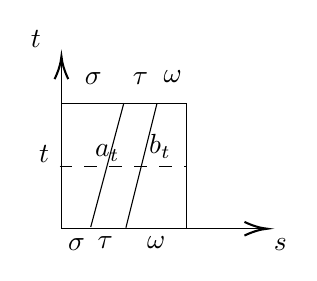
\begin{tikzpicture}[x=0.75pt,y=0.75pt,yscale=-1,xscale=1]
    %uncomment if require: \path (0,202); %set diagram left start at 0, and has height of 202
    
    %Straight Lines [id:da04747425940026373] 
    \draw    (120,140) -- (120,58.97) ;
    \draw [shift={(120,56.97)}, rotate = 90] [color={rgb, 255:red, 0; green, 0; blue, 0 }  ][line width=0.75]    (10.93,-3.29) .. controls (6.95,-1.4) and (3.31,-0.3) .. (0,0) .. controls (3.31,0.3) and (6.95,1.4) .. (10.93,3.29)   ;
    %Straight Lines [id:da3219629386493783] 
    \draw    (120,140) -- (217.11,140) ;
    \draw [shift={(219.11,140)}, rotate = 180] [color={rgb, 255:red, 0; green, 0; blue, 0 }  ][line width=0.75]    (10.93,-3.29) .. controls (6.95,-1.4) and (3.31,-0.3) .. (0,0) .. controls (3.31,0.3) and (6.95,1.4) .. (10.93,3.29)   ;
    %Straight Lines [id:da9931172020798975] 
    \draw    (120,79.49) -- (180.11,79.49) ;
    %Straight Lines [id:da8434683594079744] 
    \draw    (180.11,79.49) -- (180.11,140.19) ;
    %Straight Lines [id:da8799143647172114] 
    \draw    (150.06,79.49) -- (134.11,139.19) ;
    %Straight Lines [id:da15033802259086904] 
    \draw    (166.06,79.49) -- (151.06,139.49) ;
    %Straight Lines [id:da14271700034761436] 
    \draw  [dash pattern={on 4.5pt off 4.5pt}]  (119.11,109.84) -- (180.11,109.84) ;
    
    % Text Node
    \draw (104,43.4) node [anchor=north west][inner sep=0.75pt]    {$t$};
    % Text Node
    \draw (221.11,143.4) node [anchor=north west][inner sep=0.75pt]    {$s$};
    % Text Node
    \draw (122,143.4) node [anchor=north west][inner sep=0.75pt]    {$\sigma $};
    % Text Node
    \draw (136.11,142.59) node [anchor=north west][inner sep=0.75pt]    {$\tau $};
    % Text Node
    \draw (160,142.4) node [anchor=north west][inner sep=0.75pt]    {$\omega $};
    % Text Node
    \draw (168,62.4) node [anchor=north west][inner sep=0.75pt]    {$\omega $};
    % Text Node
    \draw (153.11,63.59) node [anchor=north west][inner sep=0.75pt]    {$\tau $};
    % Text Node
    \draw (130,63.4) node [anchor=north west][inner sep=0.75pt]    {$\sigma $};
    % Text Node
    \draw (108,98.4) node [anchor=north west][inner sep=0.75pt]    {$t$};
    % Text Node
    \draw (135,98.4) node [anchor=north west][inner sep=0.75pt]    {$a_{t}$};
    % Text Node
    \draw (161,93.4) node [anchor=north west][inner sep=0.75pt]    {$b_{t}$};
    \end{tikzpicture}\]
不妨令$F :I \times I \to X$在固定$t$时刻后
$$
F(s,t) = \left\{
\begin{array}{c}
    \sigma(\frac{s}{a_t}) , 0\leq s \leq a_t\\
    \tau(\frac{s-a_t}{b_t - a_t}), a_t \leq s \leq b_t\\
    \omega(\frac{s-b_t}{1-b_t}),b_t \leq s \leq 1\\
    \end{array}
\right.
$$
得到$F(s,0) = (\sigma\cdot \tau) \cdot \omega(s)$,$F(s,1) = \sigma \cdot(\tau \cdot \omega)(s)$且$F(0,t) = x_0$,$F(1,t) = x_3$.
因此$F$是$(\sigma \cdot \tau) \cdot \omega$到$\sigma \cdot (\tau \cdot \omega)$的道路伦移.
\end{proof}
既然道路的合成在同伦层面上满足结合律,根据商映射的思想,我们或许可以将道路同伦类转化为一个代表元道路进行考虑.首先要给道路同伦类进行一个明确的定义.
\begin{definition}
    以$x_0$为起终点的闭路关于道路同伦的所有等价类集$\Omega X / \simeq_p$记为$\pi_1(X,x_0)$,其元素为闭路的等价类$[\sigma] := \{\tau: \tau \simeq_p \sigma\}$,$\sigma$称为$[\sigma]$的一个代表元.
\end{definition}
根据定义不难得到$\sigma \simeq_p \tau \Leftrightarrow [\sigma] = [\tau]$.


那么,根据引理\ref{lem:2.3.1}可以得到当$\sigma \simeq_p \sigma'$且$\tau \simeq_p \tau'$时有$\sigma \cdot \tau \simeq_p \sigma' \cdot \tau'$.这说明$[\sigma \cdot\tau] = [\sigma' \cdot \tau']$.


很自然地,延续先前的思想,打算在$\pi_1(X,x_0)$上定义一个乘法.
\begin{definition}
    在$\pi_1(X,x_0)$定义乘法"$\cdot$":$[\sigma]\cdot[\tau] = [\sigma \cdot\tau]$.
\end{definition}
我们希望$\pi_1(X,x_0)$能够在"$\cdot$"下构成一个群.\\
在构成群之前,需要定义一个幺元,
\begin{lemma}
    $c_{x_0} : I \times X$为一个常值映射,$\forall s \in I$,$c_{x_0}(s) = x_0$.是$\pi_1(X,x_0)$的幺元.
    \label{lem:2.3.3}
\end{lemma}
\begin{proof}
    欲证$c_{x_0}$为一个左幺元.即证$[c_{x_0}][\sigma] = [c_{x_0}\cdot \sigma] = [\sigma]$这无非是在说$c_{x_0} \cdot \sigma \simeq_p \sigma$.\\
    考虑\[\tikzset{every picture/.style={line width=0.75pt}} %set default line width to 0.75pt        
    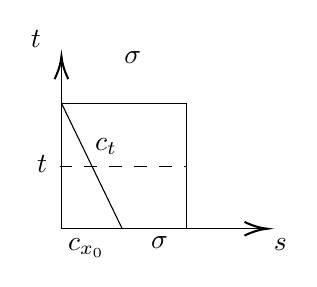
\begin{tikzpicture}[x=0.75pt,y=0.75pt,yscale=-1,xscale=1]
    %uncomment if require: \path (0,300); %set diagram left start at 0, and has height of 300
    
    %Straight Lines [id:da19291644418943243] 
    \draw    (140,160) -- (140,78.97) ;
    \draw [shift={(140,76.97)}, rotate = 90] [color={rgb, 255:red, 0; green, 0; blue, 0 }  ][line width=0.75]    (10.93,-3.29) .. controls (6.95,-1.4) and (3.31,-0.3) .. (0,0) .. controls (3.31,0.3) and (6.95,1.4) .. (10.93,3.29)   ;
    %Straight Lines [id:da6168966791216064] 
    \draw    (140,160) -- (237.11,160) ;
    \draw [shift={(239.11,160)}, rotate = 180] [color={rgb, 255:red, 0; green, 0; blue, 0 }  ][line width=0.75]    (10.93,-3.29) .. controls (6.95,-1.4) and (3.31,-0.3) .. (0,0) .. controls (3.31,0.3) and (6.95,1.4) .. (10.93,3.29)   ;
    %Straight Lines [id:da4782473849485722] 
    \draw    (140,99.49) -- (200.11,99.49) ;
    %Straight Lines [id:da8618500508034459] 
    \draw    (200.11,99.49) -- (200.11,160.19) ;
    %Straight Lines [id:da4760533810114089] 
    \draw  [dash pattern={on 4.5pt off 4.5pt}]  (139.11,129.84) -- (200.11,129.84) ;
    %Straight Lines [id:da8985714233088198] 
    \draw    (169.11,159.65) -- (140,99.49) ;
    
    % Text Node
    \draw (124,63.4) node [anchor=north west][inner sep=0.75pt]    {$t$};
    % Text Node
    \draw (241.11,163.4) node [anchor=north west][inner sep=0.75pt]    {$s$};
    % Text Node
    \draw (127,123.4) node [anchor=north west][inner sep=0.75pt]    {$t$};
    % Text Node
    \draw (182,162.4) node [anchor=north west][inner sep=0.75pt]    {$\sigma $};
    % Text Node
    \draw (169,73.4) node [anchor=north west][inner sep=0.75pt]    {$\sigma $};
    % Text Node
    \draw (142,163.4) node [anchor=north west][inner sep=0.75pt]    {$c_{x_{0}}$};
    % Text Node
    \draw (155,115.4) node [anchor=north west][inner sep=0.75pt]    {$c_{t}$};
    \end{tikzpicture}\]
    令$F : I \times I \to X$,在固定$t$时为
    $$
    F(s,t) = \left\{
        \begin{array}{c}
            c_{x_0}(\frac{s}{c_t}),0\leq s \leq c_t\\
            \sigma(\frac{s-c_t}{1-c_t}),c_t \leq s\leq 1\\
        \end{array}
    \right.
    $$
    得到$F(s,0) = c_{x_0}\cdot \sigma(s)$,$F(s,1) = \sigma(s)$,$F(0,t) = x_0 = F(1,t)$


    因此$c_{x_0} \cdot \sigma \simeq_p \sigma$,即$c_{x_0}$是一个左幺元.右幺元的情况类似可证.
\end{proof}
此时$\pi_1(X,x_0)$成功地变成了一个幺半群,距离它变成一个群还差一点——逆元.
\begin{lemma}
    对于任意的$[\sigma] \in \pi_1(X,x_0)$有$\sigma^{-1}: I \to X$,使得$\sigma^{-1}(s) = \sigma(1-s)$,$[\sigma^{-1}]$是$[\sigma]$的逆元.
    \label{lem:2.3.4}
\end{lemma}
\begin{proof}
    若$\sigma^{-1}$是$\sigma$的左逆元,则$[\sigma^{-1}][\sigma] = [\sigma^{-1}\sigma] = [c_{x_0}]$.即证$\sigma^{-1}\sigma \simeq_p c_{x_0}$.
    考虑
    \[\tikzset{every picture/.style={line width=0.75pt}} %set default line width to 0.75pt        
    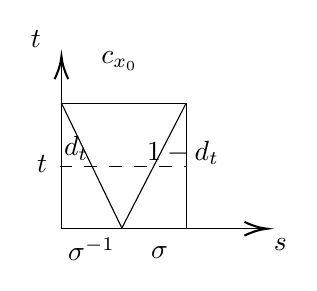
\begin{tikzpicture}[x=0.75pt,y=0.75pt,yscale=-1,xscale=1]
    %uncomment if require: \path (0,300); %set diagram left start at 0, and has height of 300
    
    %Straight Lines [id:da19291644418943243] 
    \draw    (140,160) -- (140,78.97) ;
    \draw [shift={(140,76.97)}, rotate = 90] [color={rgb, 255:red, 0; green, 0; blue, 0 }  ][line width=0.75]    (10.93,-3.29) .. controls (6.95,-1.4) and (3.31,-0.3) .. (0,0) .. controls (3.31,0.3) and (6.95,1.4) .. (10.93,3.29)   ;
    %Straight Lines [id:da6168966791216064] 
    \draw    (140,160) -- (237.11,160) ;
    \draw [shift={(239.11,160)}, rotate = 180] [color={rgb, 255:red, 0; green, 0; blue, 0 }  ][line width=0.75]    (10.93,-3.29) .. controls (6.95,-1.4) and (3.31,-0.3) .. (0,0) .. controls (3.31,0.3) and (6.95,1.4) .. (10.93,3.29)   ;
    %Straight Lines [id:da4782473849485722] 
    \draw    (140,99.49) -- (200.11,99.49) ;
    %Straight Lines [id:da8618500508034459] 
    \draw    (200.11,99.49) -- (200.11,160.19) ;
    %Straight Lines [id:da4760533810114089] 
    \draw  [dash pattern={on 4.5pt off 4.5pt}]  (139.11,129.84) -- (200.11,129.84) ;
    %Straight Lines [id:da8985714233088198] 
    \draw    (169.11,159.65) -- (140,99.49) ;
    %Straight Lines [id:da8912683354343096] 
    \draw    (169.11,159.65) -- (200.11,99.49) ;
    
    % Text Node
    \draw (124,63.4) node [anchor=north west][inner sep=0.75pt]    {$t$};
    % Text Node
    \draw (241.11,163.4) node [anchor=north west][inner sep=0.75pt]    {$s$};
    % Text Node
    \draw (127,123.4) node [anchor=north west][inner sep=0.75pt]    {$t$};
    % Text Node
    \draw (182,167.4) node [anchor=north west][inner sep=0.75pt]    {$\sigma$};
    % Text Node
    \draw (158,73.4) node [anchor=north west][inner sep=0.75pt]    {$c_{x_{0}}$};
    % Text Node
    \draw (142,163.4) node [anchor=north west][inner sep=0.75pt]    {$\sigma ^{-1}$};
    % Text Node
    \draw (140,114.4) node [anchor=north west][inner sep=0.75pt]    {$d_{t}$};
    % Text Node
    \draw (180,116.4) node [anchor=north west][inner sep=0.75pt]    {$1-d_{t}$};
    \end{tikzpicture}\]
    构建$F: I \times I \to X$,固定$t$时,
    $$
    F(s,t) = \left\{
        \begin{array}{c}
            \sigma^{-1}(2s) , 0\leq s \leq d_t\\
            \sigma^{-1}(2d_t) = \sigma(1-2d_t),d_t \leq s \leq 1-d_t\\
            \sigma(2s -1), 1-d_t \leq s \leq 1\\
        \end{array}
    \right.
    $$
    由于$F(s,1) = x_0$,$F(s,0) = \sigma^{-1} \sigma(s)$而$F(0,t) = F(1,t) =x_0$因此$\sigma^{-1} \sigma \simeq_p c_{x_0}$.因此$[\sigma^{-1}]$是$[\sigma]$的左逆,右逆的情况类似可证.

\end{proof}
\begin{theorem}
    $\pi_1(X,x_0)$在"$\cdot$"下构成一个群,称为$X$的基本群(一般来说不交换)
\end{theorem}
\begin{proof}
    封闭性: $\forall [\sigma],[\tau] \in \pi_1(X,x_0)$有$[\sigma]\cdot [\tau] = [\sigma \cdot \tau] \in \pi_1(X,x_0)$.\\
    结合律: $([\sigma]\cdot [\tau])\cdot [\omega] = [(\sigma \cdot \tau)\cdot \omega]$,$[\sigma]\cdot([\tau]\cdot [\omega]) = [\sigma \cdot (\tau \cdot \omega)]$.由于$(\sigma \cdot \tau)\cdot \omega \simeq_p \sigma\cdot(\tau \cdot \omega)$.因此得到$[(\sigma \cdot \tau)\cdot \omega] =[\sigma \cdot (\tau \cdot \omega)]$.\\
    单位元(幺元):  $c_{x_0} : I \times X$为一个常值映射,$\forall s \in I$,$c_{x_0}(s) = x_0$.根据引理\ref{lem:2.3.3}可知$c_{x_0}$是$\pi_1(X,x_0)$的幺元.\\
    逆元: 根据引理\ref{lem:2.3.4}可知$\sigma^{-1}(s) := \sigma(1-s)$的等价类$[\sigma^{-1}]$是$[\sigma]$的逆元.\\
    因此$\pi_1(X,x_0)$构成一个群.
\end{proof}
并不是所有的基本群都是非平凡的.对于基本群为平凡群的拓扑空间,我们称其为单连通的.
\begin{example}
    考虑$0 \in \mathbb{R}^n$有$\pi_1(\mathbb{R}^n,0) = \{[e]\}$\\
    这是因为对于任意的$\sigma \in \Omega X$.
    \[\tikzset{every picture/.style={line width=0.75pt}} %set default line width to 0.75pt        
    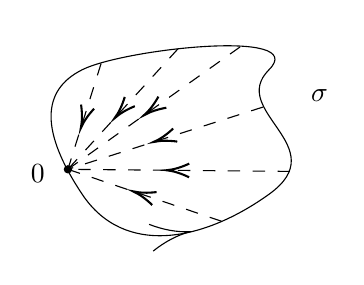
\begin{tikzpicture}[x=0.75pt,y=0.75pt,yscale=-1,xscale=1]
    %uncomment if require: \path (0,199); %set diagram left start at 0, and has height of 199
    
    %Shape: Polygon Curved [id:ds8497521177851743] 
    \draw   (140,58) .. controls (160,48) and (250,38) .. (230,58) .. controls (210,78) and (262.11,94.98) .. (230,118) .. controls (197.89,141.02) and (160,148) .. (140,118) .. controls (120,88) and (120,68) .. (140,58) -- cycle ;
    %Shape: Free Drawing [id:dp9025273576596802] 
    \draw  [line width=3] [line join = round][line cap = round] (133.11,105.98) .. controls (133.11,105.98) and (133.11,105.98) .. (133.11,105.98) ;
    \draw   (172.23,132.49) .. controls (179.01,135.11) and (185.55,136.3) .. (191.89,136.05) .. controls (185.77,137.72) and (179.89,140.82) .. (174.21,145.36) ;
    %Straight Lines [id:da4703503910238467] 
    \draw  [dash pattern={on 4.5pt off 4.5pt}]  (149.11,54.98) -- (133.11,105.98) ;
    \draw [shift={(139.32,86.2)}, rotate = 287.42] [color={rgb, 255:red, 0; green, 0; blue, 0 }  ][line width=0.75]    (10.93,-3.29) .. controls (6.95,-1.4) and (3.31,-0.3) .. (0,0) .. controls (3.31,0.3) and (6.95,1.4) .. (10.93,3.29)   ;
    %Straight Lines [id:da573484188414934] 
    \draw  [dash pattern={on 4.5pt off 4.5pt}]  (186.11,47.98) -- (133.11,105.98) ;
    \draw [shift={(155.56,81.41)}, rotate = 312.42] [color={rgb, 255:red, 0; green, 0; blue, 0 }  ][line width=0.75]    (10.93,-3.29) .. controls (6.95,-1.4) and (3.31,-0.3) .. (0,0) .. controls (3.31,0.3) and (6.95,1.4) .. (10.93,3.29)   ;
    %Straight Lines [id:da973678317753256] 
    \draw  [dash pattern={on 4.5pt off 4.5pt}]  (216.11,46.98) -- (133.11,105.98) ;
    \draw [shift={(169.72,79.96)}, rotate = 324.59] [color={rgb, 255:red, 0; green, 0; blue, 0 }  ][line width=0.75]    (10.93,-3.29) .. controls (6.95,-1.4) and (3.31,-0.3) .. (0,0) .. controls (3.31,0.3) and (6.95,1.4) .. (10.93,3.29)   ;
    %Straight Lines [id:da6972031846506068] 
    \draw  [dash pattern={on 4.5pt off 4.5pt}]  (227.11,75.98) -- (133.11,105.98) ;
    \draw [shift={(174.4,92.8)}, rotate = 342.3] [color={rgb, 255:red, 0; green, 0; blue, 0 }  ][line width=0.75]    (10.93,-3.29) .. controls (6.95,-1.4) and (3.31,-0.3) .. (0,0) .. controls (3.31,0.3) and (6.95,1.4) .. (10.93,3.29)   ;
    %Straight Lines [id:da8216272709289776] 
    \draw  [dash pattern={on 4.5pt off 4.5pt}]  (240.11,106.98) -- (133.11,105.98) ;
    \draw [shift={(180.61,106.42)}, rotate = 0.54] [color={rgb, 255:red, 0; green, 0; blue, 0 }  ][line width=0.75]    (10.93,-3.29) .. controls (6.95,-1.4) and (3.31,-0.3) .. (0,0) .. controls (3.31,0.3) and (6.95,1.4) .. (10.93,3.29)   ;
    %Straight Lines [id:da13537795611629533] 
    \draw  [dash pattern={on 4.5pt off 4.5pt}]  (207.11,130.98) -- (133.11,105.98) ;
    \draw [shift={(164.43,116.56)}, rotate = 18.67] [color={rgb, 255:red, 0; green, 0; blue, 0 }  ][line width=0.75]    (10.93,-3.29) .. controls (6.95,-1.4) and (3.31,-0.3) .. (0,0) .. controls (3.31,0.3) and (6.95,1.4) .. (10.93,3.29)   ;
    
    % Text Node
    \draw (249,66.4) node [anchor=north west][inner sep=0.75pt]    {$\sigma $};
    % Text Node
    \draw (114,102.4) node [anchor=north west][inner sep=0.75pt]    {$0$};
    \end{tikzpicture}\]
    可以构建$F : I \times I \to X$使得$F(s,t) = (1-t)\sigma(s)$.
\end{example}
\begin{theorem}
    对于任何群$G$,都存在拓扑空间$X$使得$\pi_1(X,x_0) \cong G$.
\end{theorem}

\subsection{基本群的性质}
不难发现基本群可以写成所有带基点的拓扑空间所构成的范畴$\bold{Top_*}$到全体群所构成的范畴$\bold{Grp}$的一个函子
$$
\pi_1(\cdot) : (X,x_0) \to \pi_1(X,x_0)
$$
设$f$是一个映射$(X,x_0) \to (Y,y_0)$,则对$X$中的闭路$\sigma : I \to X$有$\sigma(0) = \sigma(1) = x_0$.有
\[\begin{tikzcd}
	I && X \\
	\\
	&& Y
	\arrow["\sigma", from=1-1, to=1-3]
	\arrow["f", from=1-3, to=3-3]
	\arrow["{f \circ \sigma}"', from=1-1, to=3-3]
\end{tikzcd}\]
此时$f\circ \sigma(0) = f\circ \sigma (1) = f(x_0) = y_0$.是$Y$中的闭路.

\begin{lemma}
    若$X$中的两条道路$\sigma$与$\tau$是道路同伦的,则$f \circ \sigma \simeq_p f \circ \tau$.
    \[\tikzset{every picture/.style={line width=0.75pt}} %set default line width to 0.75pt        
    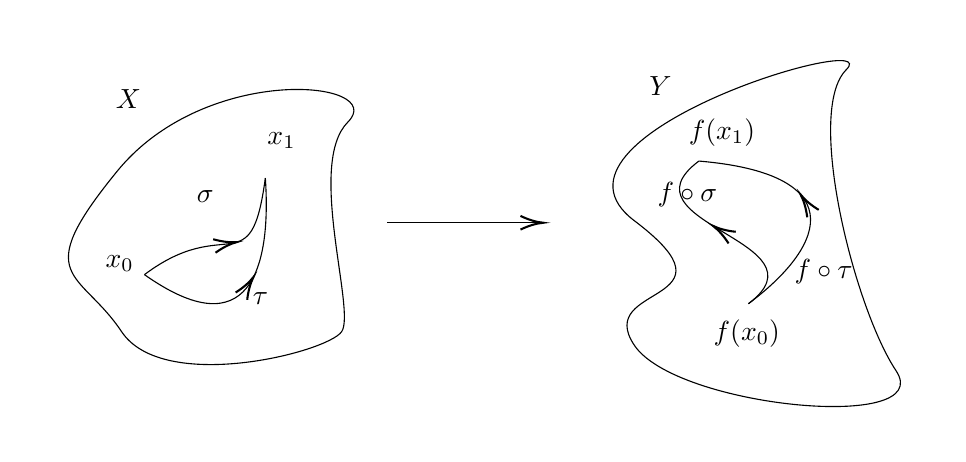
\begin{tikzpicture}[x=0.75pt,y=0.75pt,yscale=-1,xscale=1]
    %uncomment if require: \path (0,199); %set diagram left start at 0, and has height of 199
    
    %Curve Lines [id:da06870559142377042] 
    \draw    (71,129) .. controls (121.24,164.45) and (132.24,126.45) .. (129.24,82.45) ;
    \draw [shift={(123.54,130.12)}, rotate = 122.21] [color={rgb, 255:red, 0; green, 0; blue, 0 }  ][line width=0.75]    (10.93,-3.29) .. controls (6.95,-1.4) and (3.31,-0.3) .. (0,0) .. controls (3.31,0.3) and (6.95,1.4) .. (10.93,3.29)   ;
    %Curve Lines [id:da03251989569283409] 
    \draw    (71,129) .. controls (111,99) and (122.24,134.45) .. (129.24,82.45) ;
    \draw [shift={(115.45,113.32)}, rotate = 170.17] [color={rgb, 255:red, 0; green, 0; blue, 0 }  ][line width=0.75]    (10.93,-3.29) .. controls (6.95,-1.4) and (3.31,-0.3) .. (0,0) .. controls (3.31,0.3) and (6.95,1.4) .. (10.93,3.29)   ;
    %Shape: Polygon Curved [id:ds048370975326988086] 
    \draw   (58,79) .. controls (101,26.49) and (189,35.49) .. (169,55.49) .. controls (149,75.49) and (173,146.49) .. (166,156.49) .. controls (159,166.49) and (80,186.49) .. (60,156.49) .. controls (40,126.49) and (15,131.51) .. (58,79) -- cycle ;
    %Straight Lines [id:da6508973504868432] 
    \draw    (188,104) -- (261.11,104) ;
    \draw [shift={(263.11,104)}, rotate = 180] [color={rgb, 255:red, 0; green, 0; blue, 0 }  ][line width=0.75]    (10.93,-3.29) .. controls (6.95,-1.4) and (3.31,-0.3) .. (0,0) .. controls (3.31,0.3) and (6.95,1.4) .. (10.93,3.29)   ;
    %Shape: Polygon Curved [id:ds167148134718476] 
    \draw   (307,103) .. controls (253.11,62.28) and (429.11,10.28) .. (409.11,30.28) .. controls (389.11,50.28) and (413.11,145.28) .. (433.11,175.28) .. controls (453.11,205.28) and (327,193) .. (307,163) .. controls (287,133) and (360.89,143.72) .. (307,103) -- cycle ;
    %Curve Lines [id:da7097567503859206] 
    \draw    (362,143) .. controls (402,113) and (298.11,104.28) .. (338.11,74.28) ;
    \draw [shift={(344.83,105.44)}, rotate = 31.54] [color={rgb, 255:red, 0; green, 0; blue, 0 }  ][line width=0.75]    (10.93,-3.29) .. controls (6.95,-1.4) and (3.31,-0.3) .. (0,0) .. controls (3.31,0.3) and (6.95,1.4) .. (10.93,3.29)   ;
    %Curve Lines [id:da238430296934657] 
    \draw    (362,143) .. controls (402,113) and (409.11,80.28) .. (338.11,74.28) ;
    \draw [shift={(387.13,90.42)}, rotate = 56.97] [color={rgb, 255:red, 0; green, 0; blue, 0 }  ][line width=0.75]    (10.93,-3.29) .. controls (6.95,-1.4) and (3.31,-0.3) .. (0,0) .. controls (3.31,0.3) and (6.95,1.4) .. (10.93,3.29)   ;
    
    % Text Node
    \draw (95,87.4) node [anchor=north west][inner sep=0.75pt]    {$\sigma $};
    % Text Node
    \draw (51,118.4) node [anchor=north west][inner sep=0.75pt]    {$x_{0}$};
    % Text Node
    \draw (129,59.4) node [anchor=north west][inner sep=0.75pt]    {$x_{1}$};
    % Text Node
    \draw (122,136.4) node [anchor=north west][inner sep=0.75pt]    {$\tau $};
    % Text Node
    \draw (56,38.4) node [anchor=north west][inner sep=0.75pt]    {$X$};
    % Text Node
    \draw (332,52.4) node [anchor=north west][inner sep=0.75pt]    {$f( x_{1})$};
    % Text Node
    \draw (344,149.4) node [anchor=north west][inner sep=0.75pt]    {$f( x_{0})$};
    % Text Node
    \draw (317,83.4) node [anchor=north west][inner sep=0.75pt]    {$f\circ \sigma $};
    % Text Node
    \draw (383,120.4) node [anchor=north west][inner sep=0.75pt]    {$f\circ \tau $};
    % Text Node
    \draw (313,32.4) node [anchor=north west][inner sep=0.75pt]    {$Y$};
    \end{tikzpicture}\]
\end{lemma}
\begin{proof}
    设$F$是从$\sigma$到$\tau$的道路伦移$F : I \times I \to X$,有$F(s,0) = \sigma(s)$,$F(s,1) = \tau(s)$,$F(0,t) = x_0$,$F(1,t) = x_1$.


    考虑复合$f \circ F$有
    \[\begin{tikzcd}
        {I\times I} && X \\
        \\
        && Y
        \arrow["F", from=1-1, to=1-3]
        \arrow["f", from=1-3, to=3-3]
        \arrow["{f \circ F}"', from=1-1, to=3-3]
    \end{tikzcd}\]
    $f \circ F : f \circ \sigma \to f\circ \tau$为道路伦移.因此$f \circ \sigma \simeq_p f \circ \tau$.
\end{proof}
对于$[\sigma] \in \pi_1(X,x_0)$,若$\sigma,\tau \in [\sigma]$则$f \circ\sigma \simeq f \circ \tau$即$[f \circ \sigma] = [f \circ \tau] \in \pi_1(Y,y_0)$.\\
因此可以由$f$定义一个$\pi_1(X,x_0)$到$\pi_1(Y,y_0)$的映射$f_*$.
\begin{definition}
    设$f : (X,x_0) \to (Y,y_0)$,定义$\pi_1(X,x_0)$到$\pi_1(Y,y_0)$的映射$f_*$.对于$\pi_1(X,x_0)$中的任意元$[\sigma]$有$f_*([\sigma]) = [f \circ \sigma] \in \pi_1(Y,y_0)$.
\end{definition}
既然得到了$f_*$,且它是两个基本群之间的映射.因此可以试着验证一下它是否为一个群同态.
\begin{lemma}
    $f : X \to Y$导出基本群的同态$f_*:\pi_1(X,x_0) \to \pi_1(Y,y_0)$是群同态.且满足\\
    i) 对$f : X \to Y$,$g : Y \to Z$,有
    $$
    (g \circ f)_* = g_* \circ f_*
    $$
    即下列图交换
    \[\begin{tikzcd}
        {(X,x_0)} && {(Y,y_0)} && {\pi_1(X,x_0)} && {\pi_1(Y,y_0)} \\
        &&& \Rightarrow \\
        && {(Z,z_0)} &&&& {\pi_1(Z,z_0)}
        \arrow["{f_*}", from=1-5, to=1-7]
        \arrow["{g_*}", from=1-7, to=3-7]
        \arrow["{(g \circ f)_*}"', from=1-5, to=3-7]
        \arrow["f", from=1-1, to=1-3]
        \arrow["g", from=1-3, to=3-3]
        \arrow["{g \circ f}"', from=1-1, to=3-3]
    \end{tikzcd}\]\\
    ii) $\text{id}_X : X \to X$导出的$(\text{id}_X)_* = \text{id} : \pi_1(X,x_0) \to \pi_1(X,x_0)$
\end{lemma}
\begin{proof}
    对任意的$[\sigma],[\tau]\in \pi_1(X,x_0)$.若$f_*$为一个群同态,则有$f_*([\sigma][\tau]) = f_*([\sigma])f_*([\tau]) = [f\sigma][f\tau]$.\\
    $$
    f_*([\sigma][\tau]) = f_*([\sigma\circ \tau]) = [f\cdot(\sigma\circ\tau)]
    $$
    因此只需要证明$[f\cdot(\sigma \circ \tau)] = [f\sigma \circ f\tau]$即可.
    $$
    f\circ(\sigma \circ \tau)(s) = \left\{
        \begin{array}{c}
            f \circ \sigma(2s),0\leq s \leq 1/2\\
            f \circ \tau(2s - 1), 1/2 \leq s \leq 1\\
        \end{array}
    \right.
    $$
    因此$[f\cdot(\sigma \circ \tau)] = [f\sigma \circ f \tau]$,即$f_*$是一个群同态,后面两条性质是显然的.
\end{proof}
\subsubsection{基本群是同胚不变量}
\begin{theorem}
    如果$X$与$Y$是两个同胚的道路连通的拓扑空间,那么它们的基本群$\pi_1(X,x_0),\pi_1(Y,y_0)$同构.
\end{theorem}
\begin{proof}
    由于$X$与$Y$同胚,因此可以找到同胚映射$f : X \xrightarrow{\cong} Y$以及其逆$g : Y \to X$使得$g \circ f = \text{id}_X$且$f \circ g = \text{id}_Y$.
    因此得到
    \[\begin{tikzcd}
        {(X,x_0)} && {(Y,y_0)} && {\pi_1(X,x_0)} && {\pi_1(Y,y_0)} \\
        &&& \Rightarrow \\
        && {(X,x_0)} &&&& {\pi_1(X,x_0)}
        \arrow["{f_*}", from=1-5, to=1-7]
        \arrow["{g_*}", from=1-7, to=3-7]
        \arrow["{(g \circ f)_*= \text{id}}"', from=1-5, to=3-7]
        \arrow["f", from=1-1, to=1-3]
        \arrow["g", from=1-3, to=3-3]
        \arrow["{g \circ f = \text{id}_X}"', from=1-1, to=3-3]
    \end{tikzcd}\]
    即$f_*$与$g_*$均为双射,又因为$f_*$为群同态,因此$f_*$为群同构,即$\pi_1(X,x_0)$与$\pi_1(Y,y_0)$同构.
\end{proof}
因此得知,基本群反映了空间的拓扑性质,是拓扑空间中的同胚不变量.
\subsubsection{基本群是同伦不变量}
接下来观察基本群是否是同伦不变量(设$f : (X,x_0) \to (Y,y_0)$,$g: (Y,y_0) \to (X,x_1)$满足$g \circ f \simeq \text{id}_X$以及$f \circ g \simeq \text{id}_Y$,则$f_*$与$g_*$均为同构)
\begin{lemma}
    若$f \simeq_p g : (X,x_0) \to (Y,y_0)$则$f_* = g_*: \pi_1(X,x_0) \to \pi_1(Y,y_0)$且$f$到$g$的伦移$F : X \times I \to Y$应当满足对任意的$t \in I$有$F(x_0,t) \equiv y_0$.
\end{lemma}
\begin{proof}
    设$F :X \times I \to Y$为$f$到$g$的伦移,由于$f$与$g$是空间偶映射之间的同伦,因此对任意的$t \in I$,$f(x_0,t) \equiv y_0$.\\
    欲证$f_* = g_*$,即证对于任意的$[\sigma]\in \pi_1(X,x_0)$有$f_*([\sigma]) = g_*([\sigma])$.即$[f\sigma] = [g \sigma]\Rightarrow f \sigma \simeq_p g \sigma$.\\
    定义$H : I \times I \to Y$使以下图表交换
    \[\begin{tikzcd}
        {I \times I} && {X \times I} \\
        \\
        && Y
        \arrow["F", from=1-3, to=3-3]
        \arrow["{\sigma \times 1}", from=1-1, to=1-3]
        \arrow["H"', from=1-1, to=3-3]
    \end{tikzcd}\]
    只需要令$H(s,t) = F(\sigma(s),t)$,就得到$H(0,t) = F(\sigma(0) ,t) \equiv t_0 \equiv H(1,t) = F(\sigma(1),t)$.且$H(s,0) = f(\sigma(s))$,$H(s,1) = g(\sigma(s))$因此得到$f\sigma \simeq_p g \sigma$.
\end{proof}
\begin{corollary}
    若$f : (X,x_0)\xrightarrow{\simeq} (Y,y_0)$是同伦等价,且$g : (Y,y_0) \to (X,x_0)$是其同伦逆.有\\
    \[\begin{tikzcd}
        {(X,x_0)} && {(Y,y_0)} && {(Y,y_0)} && {(X,x_0)} \\
        \\
        && {(X,x_0)} &&&& {(Y,y_0)}
        \arrow["g", from=1-5, to=1-7]
        \arrow["f", from=1-7, to=3-7]
        \arrow["{\simeq 1_{(Y,y_0)}}"', from=1-5, to=3-7]
        \arrow["f", from=1-1, to=1-3]
        \arrow["{\simeq 1_{(X,x_0)}}"', from=1-1, to=3-3]
        \arrow["g", from=1-3, to=3-3]
    \end{tikzcd}\]
    则
    \[\begin{tikzcd}
        {\pi_1(X,x_0)} && {\pi_1(Y,y_0)} && {\pi_1(Y,y_0)} && {\pi_1(X,x_0)} \\
        \\
        && {\pi_1(X,x_0)} &&&& {\pi_1(Y,y_0)}
        \arrow["{g_*}", from=1-5, to=1-7]
        \arrow["{f_*}", from=1-7, to=3-7]
        \arrow["{\text{id}}"', from=1-5, to=3-7]
        \arrow["{f_*}", from=1-1, to=1-3]
        \arrow["{\text{id}}"', from=1-1, to=3-3]
        \arrow["{g_*}", from=1-3, to=3-3]
    \end{tikzcd}\]
\end{corollary}

    任取$x_0\in X$,且有两个同伦的映射$f,g$,$H: X \times I \to Y$是从$f$到$g$的一个伦移,记$f(x_0) = y_0$,$g(x_0) = y_0'$,存在$\gamma: I \to Y$使得$\gamma(t)  = H(x_0,t)$.
    \[\tikzset{every picture/.style={line width=0.75pt}} %set default line width to 0.75pt        
    \begin{tikzpicture}[x=0.75pt,y=0.75pt,yscale=-1,xscale=1]
    %uncomment if require: \path (0,300); %set diagram left start at 0, and has height of 300
    
    %Shape: Polygon Curved [id:ds37773380399094103] 
    \draw   (78,99) .. controls (121,46.49) and (209,55.49) .. (189,75.49) .. controls (169,95.49) and (193,166.49) .. (186,176.49) .. controls (179,186.49) and (100,206.49) .. (80,176.49) .. controls (60,146.49) and (35,151.51) .. (78,99) -- cycle ;
    %Shape: Polygon Curved [id:ds9160194930438348] 
    \draw   (327,123) .. controls (273.11,82.28) and (449.11,30.28) .. (429.11,50.28) .. controls (409.11,70.28) and (433.11,165.28) .. (453.11,195.28) .. controls (473.11,225.28) and (347,213) .. (327,183) .. controls (307,153) and (380.89,163.72) .. (327,123) -- cycle ;
    %Shape: Free Drawing [id:dp9565053855116716] 
    \draw  [line width=3] [line join = round][line cap = round] (120.11,129.54) .. controls (120.11,129.54) and (120.11,129.54) .. (120.11,129.54) ;
    %Shape: Free Drawing [id:dp4173452523503234] 
    \draw  [line width=3] [line join = round][line cap = round] (388.11,97.54) .. controls (388.11,97.54) and (388.11,97.54) .. (388.11,97.54) ;
    %Shape: Free Drawing [id:dp09692621653559708] 
    \draw  [line width=3] [line join = round][line cap = round] (389.11,177.54) .. controls (389.11,177.54) and (389.11,177.54) .. (389.11,177.54) ;
    %Straight Lines [id:da831664797000935] 
    \draw  [dash pattern={on 4.5pt off 4.5pt}]  (121.11,129.54) -- (387.13,97.78) ;
    \draw [shift={(389.11,97.54)}, rotate = 173.19] [color={rgb, 255:red, 0; green, 0; blue, 0 }  ][line width=0.75]    (10.93,-3.29) .. controls (6.95,-1.4) and (3.31,-0.3) .. (0,0) .. controls (3.31,0.3) and (6.95,1.4) .. (10.93,3.29)   ;
    %Straight Lines [id:da3606372304265042] 
    \draw  [dash pattern={on 4.5pt off 4.5pt}]  (121.11,129.54) -- (387.14,177.19) ;
    \draw [shift={(389.11,177.54)}, rotate = 190.15] [color={rgb, 255:red, 0; green, 0; blue, 0 }  ][line width=0.75]    (10.93,-3.29) .. controls (6.95,-1.4) and (3.31,-0.3) .. (0,0) .. controls (3.31,0.3) and (6.95,1.4) .. (10.93,3.29)   ;
    %Curve Lines [id:da39123878251274125] 
    \draw    (389.11,97.54) .. controls (427.11,132.54) and (354.11,156.54) .. (389.11,177.54) ;
    \draw [shift={(389.41,143.96)}, rotate = 304.61] [color={rgb, 255:red, 0; green, 0; blue, 0 }  ][line width=0.75]    (10.93,-3.29) .. controls (6.95,-1.4) and (3.31,-0.3) .. (0,0) .. controls (3.31,0.3) and (6.95,1.4) .. (10.93,3.29)   ;
    
    % Text Node
    \draw (121,106.4) node [anchor=north west][inner sep=0.75pt]    {$x_{0}$};
    % Text Node
    \draw (76,58.4) node [anchor=north west][inner sep=0.75pt]    {$X$};
    % Text Node
    \draw (333,52.4) node [anchor=north west][inner sep=0.75pt]    {$Y$};
    % Text Node
    \draw (229,97.4) node [anchor=north west][inner sep=0.75pt]    {$f$};
    % Text Node
    \draw (243,154.4) node [anchor=north west][inner sep=0.75pt]    {$g$};
    % Text Node
    \draw (392,78.4) node [anchor=north west][inner sep=0.75pt]    {$y_{0}$};
    % Text Node
    \draw (401,171.4) node [anchor=north west][inner sep=0.75pt]    {$y_{0} '$};
    % Text Node
    \draw (372,121.4) node [anchor=north west][inner sep=0.75pt]    {$\gamma $};
    
    
    \end{tikzpicture}\]
    由于前文已经导出了$f_*$和$g_*$这两个基本群之间的同态,分别映射为$Y$上的两个基本群$\pi_1(Y,y_0)$与$\pi_1(Y,y_0')$,它们之间是有联系的,为了观察这一点,接下来不再使用$X$中的道路,而是讨论$Y$上的道路建立基本群之间的联系.
    \begin{definition}
        对于$Y$中从$y_0$到$y_0'$的道路$\gamma : I \to Y$,$\gamma(0) = y_0$且$\gamma(1) = y_0'$.定义映射$\gamma_* : \pi_1(Y,y_0) \to \pi_1(Y,y_1)$.
        \[\tikzset{every picture/.style={line width=0.75pt}} %set default line width to 0.75pt        
        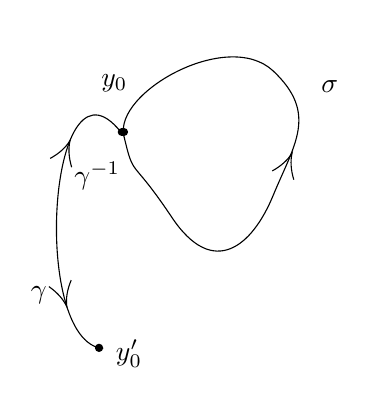
\begin{tikzpicture}[x=0.75pt,y=0.75pt,yscale=-1,xscale=1]
        %uncomment if require: \path (0,300); %set diagram left start at 0, and has height of 300
        
        %Shape: Polygon Curved [id:ds5635319154810139] 
        \draw   (158.11,96.43) .. controls (153.11,75.43) and (208.11,44.43) .. (230,65) .. controls (251.89,85.57) and (240.11,100.43) .. (230,125) .. controls (219.89,149.57) and (201.11,165.43) .. (181.11,135.43) .. controls (161.11,105.43) and (163.11,117.43) .. (158.11,96.43) -- cycle ;
        %Curve Lines [id:da6828853234933467] 
        \draw    (158.11,96.43) .. controls (122.11,46.43) and (112.11,195.76) .. (148.11,198.76) ;
        %Shape: Free Drawing [id:dp4819410348916706] 
        \draw  [line width=3] [line join = round][line cap = round] (158.11,94.43) .. controls (157.78,94.43) and (157.44,94.43) .. (157.11,94.43) ;
        %Shape: Free Drawing [id:dp43300925795200396] 
        \draw  [line width=3] [line join = round][line cap = round] (146.11,198.43) .. controls (146.11,198.43) and (146.11,198.43) .. (146.11,198.43) ;
        \draw   (132.7,165.81) .. controls (130.79,170.38) and (130.07,174.61) .. (130.54,178.48) .. controls (128.87,174.95) and (126.01,171.76) .. (121.96,168.92) ;
        \draw   (229.58,113.17) .. controls (233.91,110.77) and (237.09,107.9) .. (239.12,104.57) .. controls (238.25,108.37) and (238.51,112.65) .. (239.94,117.39) ;
        \draw   (122.57,107.16) .. controls (126.91,104.77) and (130.09,101.9) .. (132.13,98.57) .. controls (131.25,102.37) and (131.51,106.65) .. (132.92,111.4) ;
        
        % Text Node
        \draw (112,167.4) node [anchor=north west][inner sep=0.75pt]    {$\gamma $};
        % Text Node
        \draw (153,193.4) node [anchor=north west][inner sep=0.75pt]    {$y_{0} '$};
        % Text Node
        \draw (146,65.4) node [anchor=north west][inner sep=0.75pt]    {$y_{0}$};
        % Text Node
        \draw (252,68.4) node [anchor=north west][inner sep=0.75pt]    {$\sigma $};
        % Text Node
        \draw (133,107.4) node [anchor=north west][inner sep=0.75pt]    {$\gamma ^{-1}$};
        
        
        \end{tikzpicture}\]
        对于$[\sigma] \in \pi_1(Y,y_0)$有$\gamma_*([\sigma]) = [\gamma^{-1} \sigma \gamma]$
    \end{definition}
先讨论一下$\gamma_*$的定义是否合理(是否与代表元的选取有关)
    \begin{proof}
        取$\sigma,\tau \in [\sigma]$有$\sigma\simeq_p \tau$.\\
        考虑$\gamma^{-1} \sigma \gamma$与$\gamma^{-1} \tau \gamma$.\\
        由于$\sigma \simeq_p \tau$因此存在$F : I \times I \to Y$使得$F$为$\sigma$到$\tau$的道路伦移.\\
        由于$\gamma^{-1} \sigma \gamma(s) = \left\{\begin{array}{c}\gamma^{-1}(3s), 0\leq s \leq 1/3\\ \sigma(3s-1), 1/3\leq s \leq 2/3\\\gamma(3s-2), 2/3 \leq s \leq 1\\ \end{array}\right.$,并且$\gamma^{-1} \tau \gamma$也是如此,因此可以得到
        \[\tikzset{every picture/.style={line width=0.75pt}} %set default line width to 0.75pt        
        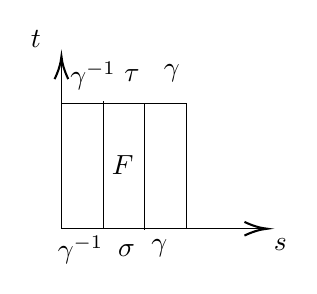
\begin{tikzpicture}[x=0.75pt,y=0.75pt,yscale=-1,xscale=1]
        %uncomment if require: \path (0,215); %set diagram left start at 0, and has height of 215
        
        %Straight Lines [id:da023674488024737705] 
        \draw    (140,160) -- (140,78.97) ;
        \draw [shift={(140,76.97)}, rotate = 90] [color={rgb, 255:red, 0; green, 0; blue, 0 }  ][line width=0.75]    (10.93,-3.29) .. controls (6.95,-1.4) and (3.31,-0.3) .. (0,0) .. controls (3.31,0.3) and (6.95,1.4) .. (10.93,3.29)   ;
        %Straight Lines [id:da2682098160398645] 
        \draw    (140,160) -- (237.11,160) ;
        \draw [shift={(239.11,160)}, rotate = 180] [color={rgb, 255:red, 0; green, 0; blue, 0 }  ][line width=0.75]    (10.93,-3.29) .. controls (6.95,-1.4) and (3.31,-0.3) .. (0,0) .. controls (3.31,0.3) and (6.95,1.4) .. (10.93,3.29)   ;
        %Straight Lines [id:da2239736895727893] 
        \draw    (140,99.49) -- (200.11,99.49) ;
        %Straight Lines [id:da959624115535711] 
        \draw    (200.11,99.49) -- (200.11,160.19) ;
        %Straight Lines [id:da35857264614699824] 
        \draw    (160.11,98.66) -- (160.11,159.66) ;
        %Straight Lines [id:da8803049896268498] 
        \draw    (180.11,99.66) -- (180.11,160.66) ;
        
        % Text Node
        \draw (124,63.4) node [anchor=north west][inner sep=0.75pt]    {$t$};
        % Text Node
        \draw (241.11,163.4) node [anchor=north west][inner sep=0.75pt]    {$s$};
        % Text Node
        \draw (137,162.4) node [anchor=north west][inner sep=0.75pt]    {$\gamma ^{-1}$};
        % Text Node
        \draw (166,166.4) node [anchor=north west][inner sep=0.75pt]    {$\sigma $};
        % Text Node
        \draw (182.11,164.06) node [anchor=north west][inner sep=0.75pt]    {$\gamma $};
        % Text Node
        \draw (143,78.18) node [anchor=north west][inner sep=0.75pt]    {$\gamma ^{-1}$};
        % Text Node
        \draw (169,82.18) node [anchor=north west][inner sep=0.75pt]    {$\tau $};
        % Text Node
        \draw (188.11,79.84) node [anchor=north west][inner sep=0.75pt]    {$\gamma $};
        % Text Node
        \draw (163,123.4) node [anchor=north west][inner sep=0.75pt]    {$F$};
        \end{tikzpicture}\]        
        不难发现可以得到一个映射
        $$
        G(s,t) = \left\{
            \begin{array}{c}
                \gamma^{-1}(3s),0\leq s \leq 1/3\\
                F(3s-1,t),1/3\leq s \leq 2/3\\
                \gamma(3s - 2), 2/3 \leq s \leq 1\\
            \end{array}
        \right.
        $$
        有$G(s,1) = \gamma^{-1}\tau \gamma(s)$,$G(s,0) = \gamma^{-1} \sigma \gamma(s)$,$G(0,t) \equiv y_0' \equiv G(1,t)$.
        因此$\gamma_*$的定义无关于代表元的选取.
    \end{proof}
    对于$\gamma_*$,它连接着$\pi_1(Y,y_0)$与$\pi_1(Y,y_0')$,为两个群之间的映射,因此其为一个群的同态,而且不难想象它还是一个同构.
    \begin{lemma}
        $\gamma_*: \pi_1(Y,y_0) \to \pi_1(Y,y_0')$是一个群同态.
        \label{lem:2.4.6}
    \end{lemma}
    \begin{proof}
        对$[\sigma],[\tau] \in \pi_1(Y,y_0)$,有$\gamma_*([\sigma][\tau]) = [\gamma^{-1} \sigma \tau \gamma]$需要证明$[\gamma^{-1} \sigma \tau \gamma] = [\gamma^{-1} \sigma\gamma][\gamma^{-1} \tau \gamma]$.这无非是要证明$\gamma^{-1}(\sigma \tau)\gamma \simeq_p \gamma^{-1}\sigma\gamma \gamma^{-1} \tau \gamma$后者同伦于$\gamma^{-1} \sigma c_{y_0} \tau \gamma$\\
        由于$c_{y_0}$为$\pi_1(Y,y_0)$上的幺元,因此$\gamma^{-1} \sigma \tau \gamma \simeq_p \gamma^{-1}\sigma c_{y_0} \tau \gamma$.
    \end{proof}
    \begin{theorem}
        对于$Y$中$y_0$到$y_1$的道路$\gamma$,其导出基本群之间的同态
        $$
        \gamma_* :\qquad \pi_1(Y,y_0) \to \pi_1(Y,y_0')
        $$
        是群同构(当$\gamma$为一个闭路时为内自同构).因此,当$Y$是一个道路连通空间时,$\pi_1(Y,y_0)$与$y_0$的选取无关,即$\pi_1(Y,y_0)$可以简记为$\pi_1(Y)$.
    \end{theorem}
    \begin{proof}
        不难发现$\gamma^{-1}(s) = \gamma(1-s)$,且其为一个$y_0'$到$y_0$的道路,因此可以构建一个$\gamma^{-1}_*$使得$\gamma^{-1}_*([\sigma']) = [\gamma \sigma' \gamma^{-1}]$对于任意的$[\sigma']\in \pi_1(Y,y_0')$成立,因此令$[\sigma'] = [\gamma^{-1}\sigma \gamma]$得到$\gamma^{-1}([\gamma^{-1}\sigma \gamma]) = [\sigma]$.\\
        换句话说:$\gamma^{-1}_*(\gamma([\sigma])) = [\sigma]$且$\gamma(\gamma^{-1}[\sigma']) = [\sigma]$.\\
        \[\begin{tikzcd}
            {\pi_1(Y,y_0)} && {\pi_1(Y,y_0')} && {\pi_1(Y,y_0')} && {\pi_1(Y,y_0)} \\
            \\
            && {\pi_1(Y,y_0)} &&&& {\pi_1(Y,y_0')}
            \arrow["{\gamma^{-1}_*}", from=1-5, to=1-7]
            \arrow["{\gamma_*}", from=1-7, to=3-7]
            \arrow["{\text{id}}"', from=1-5, to=3-7]
            \arrow["{\gamma_*}", from=1-1, to=1-3]
            \arrow["{\text{id}}"', from=1-1, to=3-3]
            \arrow["{\gamma^{-1}_*}", from=1-3, to=3-3]
        \end{tikzcd}\]
        因此根据双射的定义容易看出$\gamma_*$就是一个双射.结合引理\ref{lem:2.4.6}得到$\gamma_*$是一个同构.
    \end{proof}
    做了这些准备后,终于可以讨论基本群的同伦不变性了,当然,把考虑的范围转回$X$和$Y$这两个拓扑空间上.
    \begin{theorem}
        设$f \simeq g : X \to Y$,$H : X \times I \to Y$为$f$到$g$的伦移.$\gamma : I \to Y$,$\gamma(t) = H(x_0,t)$是从$y_0 = f(x_0)$到$y_0' = g(x_0)$的道路,则以下图表交换
        \[\begin{tikzcd}
            && {\pi_1(Y,y_0)} \\
            {\pi_1(X,x_0)} \\
            && {\pi_1(Y,y_0')}
            \arrow["{f_*}", from=2-1, to=1-3]
            \arrow["{g_*}"', from=2-1, to=3-3]
            \arrow["\gamma", dashed, from=1-3, to=3-3]
            \arrow["\cong", from=3-3, to=1-3]
        \end{tikzcd}\]
        \label{the:2.4.8}
    \end{theorem}
\begin{proof}
    若图表交换,则$\gamma_* \circ f_* ([\sigma]) = \gamma_*([f\sigma]) = [\gamma^{-1}f \sigma \gamma] = g_*([\sigma]) = [g\sigma]$.因此需要证明$\gamma^{-1} f \sigma \gamma \simeq g \sigma$.\\
    由于$f \simeq g$,因此其伦移$F$已经提供了这样的形变,记$f_t(x) = F(x,t)$且$f_0 = f,f_1 = g$,有$(f_t \circ \sigma)(t) = F(\sigma(t) ,s)$,这是以$\gamma(t) = F(x_0,t)$为起点的闭路,在$t = 0$时,它是$f_0 \circ \sigma$;在$t = 1$时,它是$f_1 \circ \sigma$.\\
    考虑
    \[\tikzset{every picture/.style={line width=0.75pt}} %set default line width to 0.75pt        
    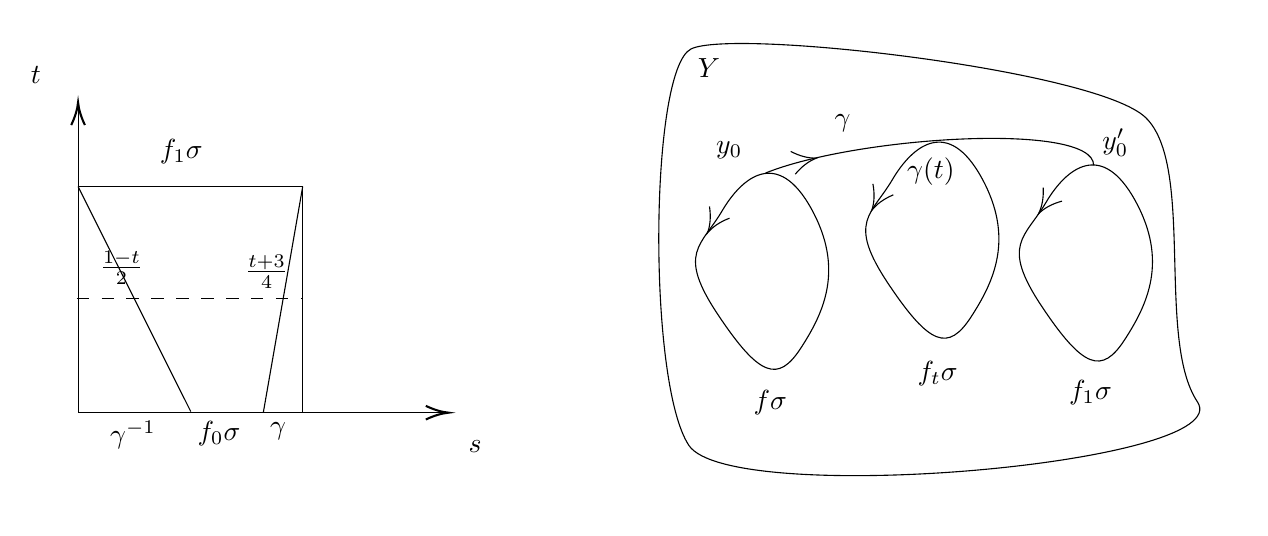
\begin{tikzpicture}[x=0.75pt,y=0.75pt,yscale=-1,xscale=1]
    %uncomment if require: \path (0,300); %set diagram left start at 0, and has height of 300
    
    %Straight Lines [id:da7326845184385022] 
    \draw    (32.81,206.45) -- (32.81,58.93) ;
    \draw [shift={(32.81,56.93)}, rotate = 90] [color={rgb, 255:red, 0; green, 0; blue, 0 }  ][line width=0.75]    (10.93,-3.29) .. controls (6.95,-1.4) and (3.31,-0.3) .. (0,0) .. controls (3.31,0.3) and (6.95,1.4) .. (10.93,3.29)   ;
    %Straight Lines [id:da354480377502957] 
    \draw    (32.81,206.45) -- (209.29,206.45) ;
    \draw [shift={(211.29,206.45)}, rotate = 180] [color={rgb, 255:red, 0; green, 0; blue, 0 }  ][line width=0.75]    (10.93,-3.29) .. controls (6.95,-1.4) and (3.31,-0.3) .. (0,0) .. controls (3.31,0.3) and (6.95,1.4) .. (10.93,3.29)   ;
    %Straight Lines [id:da4659715399167659] 
    \draw    (32.81,97.47) -- (141.05,97.47) ;
    %Straight Lines [id:da13459575898394882] 
    \draw    (141.05,97.47) -- (141.05,206.8) ;
    %Straight Lines [id:da7822766128896861] 
    \draw    (32.81,97.47) -- (87.11,205.89) ;
    %Straight Lines [id:da9471442903201657] 
    \draw    (141.05,97.47) -- (122.05,206.45) ;
    %Straight Lines [id:da6201679166743947] 
    \draw  [dash pattern={on 4.5pt off 4.5pt}]  (32.11,151.22) -- (141.05,151.22) ;
    %Shape: Polygon Curved [id:ds7494667016664387] 
    \draw   (328.11,31.22) .. controls (348.11,21.22) and (523.11,41.22) .. (547.11,64.22) .. controls (571.11,87.22) and (552.11,171.22) .. (572.11,201.22) .. controls (592.11,231.22) and (347.11,252.22) .. (327.11,222.22) .. controls (307.11,192.22) and (308.11,41.22) .. (328.11,31.22) -- cycle ;
    %Shape: Polygon Curved [id:ds36588193778139577] 
    \draw   (343.11,109.22) .. controls (353.11,92.22) and (370.11,79.22) .. (386.11,108.22) .. controls (402.11,137.22) and (392.11,158.22) .. (381.11,175.22) .. controls (370.11,192.22) and (361.11,189.22) .. (341.11,159.22) .. controls (321.11,129.22) and (333.11,126.22) .. (343.11,109.22) -- cycle ;
    %Curve Lines [id:da5554480560122492] 
    \draw    (364,91) .. controls (408.11,73.22) and (522.11,66.22) .. (522.11,87.22) ;
    %Shape: Polygon Curved [id:ds4370666312827538] 
    \draw   (425.11,94.22) .. controls (435.11,77.22) and (452.11,64.22) .. (468.11,93.22) .. controls (484.11,122.22) and (474.11,143.22) .. (463.11,160.22) .. controls (452.11,177.22) and (443.11,174.22) .. (423.11,144.22) .. controls (403.11,114.22) and (415.11,111.22) .. (425.11,94.22) -- cycle ;
    %Shape: Polygon Curved [id:ds6430484700164885] 
    \draw   (499.11,105.22) .. controls (509.11,88.22) and (526.11,75.22) .. (542.11,104.22) .. controls (558.11,133.22) and (548.11,154.22) .. (537.11,171.22) .. controls (526.11,188.22) and (517.11,185.22) .. (497.11,155.22) .. controls (477.11,125.22) and (489.11,122.22) .. (499.11,105.22) -- cycle ;
    \draw   (376.17,80.57) .. controls (380.56,82.86) and (384.71,83.93) .. (388.61,83.79) .. controls (384.96,85.16) and (381.53,87.74) .. (378.36,91.54) ;
    \draw   (346.68,112.74) .. controls (342.05,114.51) and (338.5,116.91) .. (336.02,119.92) .. controls (337.42,116.28) and (337.76,112.01) .. (337.02,107.11) ;
    \draw   (425.61,101.49) .. controls (421.04,103.41) and (417.57,105.92) .. (415.19,109.02) .. controls (416.47,105.33) and (416.66,101.05) .. (415.76,96.18) ;
    \draw   (506.86,104.52) .. controls (502.08,105.82) and (498.31,107.86) .. (495.54,110.61) .. controls (497.3,107.12) and (498.06,102.91) .. (497.8,97.96) ;
    
    % Text Node
    \draw (8.8,38.58) node [anchor=north west][inner sep=0.75pt]    {$t$};
    % Text Node
    \draw (219.69,218.66) node [anchor=north west][inner sep=0.75pt]    {$s$};
    % Text Node
    \draw (71,73.4) node [anchor=north west][inner sep=0.75pt]    {$f_{1} \sigma $};
    % Text Node
    \draw (47,209.4) node [anchor=north west][inner sep=0.75pt]    {$\gamma ^{-1}$};
    % Text Node
    \draw (89.11,209.29) node [anchor=north west][inner sep=0.75pt]    {$f_{0} \sigma $};
    % Text Node
    \draw (124.05,209.85) node [anchor=north west][inner sep=0.75pt]    {$\gamma $};
    % Text Node
    \draw (42,127.4) node [anchor=north west][inner sep=0.75pt]    {$\frac{1-t}{2}$};
    % Text Node
    \draw (112,129.4) node [anchor=north west][inner sep=0.75pt]    {$\frac{t+3}{4}$};
    % Text Node
    \draw (357,194.4) node [anchor=north west][inner sep=0.75pt]    {$f\sigma $};
    % Text Node
    \draw (436,180.4) node [anchor=north west][inner sep=0.75pt]    {$f_{t} \sigma $};
    % Text Node
    \draw (509,189.4) node [anchor=north west][inner sep=0.75pt]    {$f_{1} \sigma $};
    % Text Node
    \draw (339,74.4) node [anchor=north west][inner sep=0.75pt]    {$y_{0}$};
    % Text Node
    \draw (396,61.4) node [anchor=north west][inner sep=0.75pt]    {$\gamma $};
    % Text Node
    \draw (431,82.4) node [anchor=north west][inner sep=0.75pt]    {$\gamma ( t)$};
    % Text Node
    \draw (525,68.4) node [anchor=north west][inner sep=0.75pt]    {$y_{0} '$};
    % Text Node
    \draw (330.11,34.62) node [anchor=north west][inner sep=0.75pt]    {$Y$};
    
    
    \end{tikzpicture}\]    
    根据上图可令
    $$
    H(s,t) = \left\{
        \begin{array}{c}
            \gamma^{-1}(2s), 0\leq s \leq \frac{1-t}{2}\\
            F(\sigma(\frac{s - \frac{1-t}{2}}{\frac{t+3}{4} -\frac{1-t}{2}}),t) , \frac{1-t}{2}\leq s \leq \frac{t+3}{4}\\
            \gamma(4s - 3), \frac{t+3}{4} \leq s \leq 1\\
        \end{array}
    \right.
    $$
    计算得到
    $$
    H(s,t) = \left\{
        \begin{array}{c}
            \gamma^{-1}(2s), 0\leq s \leq \frac{1-t}{2}\\
            F(\sigma(\frac{4s+2t-2}{3t+1}),t) , \frac{1-t}{2}\leq s \leq \frac{t+3}{4}\\
            \gamma(4s - 3), \frac{t+3}{4} \leq s \leq 1\\
        \end{array}
    \right.
    $$
    不难发现$H : \gamma^{-1}(f\sigma \cdot \gamma) \simeq_p g \sigma$.
\end{proof}
\begin{corollary}
    若$f : X \xrightarrow{\simeq} Y$是同伦等价,$g : Y \to X$为其同伦逆,若$f(x_0) = y_0$则$f_* : \pi_1(X,x_0) \to \pi_1(Y,y_0)$是同构.
\label{cor:2.4.9}
\end{corollary}
\begin{proof}
    由于$f : X \xrightarrow{\simeq} Y$是同伦等价,因此存在其同伦逆$g$使得$g \circ f\simeq \text{id}_X$,而$f \circ g \simeq \text{id}_Y$.这说明下述图表等价
    \[\begin{tikzcd}
        X && Y && {\pi_1(X,x_0)} && {\pi_1(Y,y_0)} \\
        \\
        && X &&&& {\pi_1(X,x_1)}
        \arrow["f", from=1-1, to=1-3]
        \arrow["g", from=1-3, to=3-3]
        \arrow["{\simeq \text{id}_X}"', from=1-1, to=3-3]
        \arrow["{f_*}", from=1-5, to=1-7]
        \arrow["{g_*}", from=1-7, to=3-7]
        \arrow["{(g\circ f)_*}"', from=1-5, to=3-7]
    \end{tikzcd}\]
    设$g(y_0) = x_1$则有右侧图表交换.\\
    不难发现$g \circ f(x_0) = x_1$,因此可以构建一条道路$\gamma$使得$\gamma(0) = x_0$,$\gamma(1) = x_1$.进而可以发现$\gamma$所诱导的基本群之间的同态就是$(g \circ f)_*$因此$(g \circ f)_*$是一个同构.同理得到$(f \circ g)_*$也是一个同构,这也就说明$f_*$与$g_*$均为同构.
\end{proof}
\subsubsection{单连通空间}
首先回顾一下单连通的定义:若一个拓扑空间$X$的基本群是平凡的,那么它就是一个单连通空间.\\
由于一点所成的拓扑空间(可收缩空间)是单连通的.因此根据定理\ref{the:2.4.8}得到.
\begin{corollary}
    可收缩空间都是单连通的.
\end{corollary}

下面的定理给出了单连通空间的一些重要性质.记$D^2 = \{x \in \mathbb{R}^2: \|x\|\leq 1\}$是一个单位闭圆盘.$S^1$为单位元.
\begin{theorem}
    对于道路连通的拓扑空间$X$,以下几个条件是等价的:\\
    1) $X$是单连通的\\
    2) 任何映射$f : S^1 \to X$可以被扩张到$D^2$上.\\
    3) $X$中任意两条起终点相同的道路是道路同伦的.
\end{theorem}
\begin{proof}
    1)$\Rightarrow$ 2) : 设$X$是单连通空间,选取映射$p: I^2 \to D^2$,把$I^2$的三边$\{0\}\times I$,$\{1\}\times I$,$I\times \{1\}$映成$D^2$上的同一点$(1,0)$,把$I \times \{0\}$映射到$D^2$的边界$S^1$上,因此得到在$I^2$的内部$p$是一个同胚.\\
    把$S^1$上的点表示为$e^{2\pi i t}$,$t \in [0,1]$.任意映射$f :S^1 \to X$可以表示为$f(e^{2\pi t})$,由此可得$X$中的闭道路
    $$
    \tilde{f}: I \to X , \tilde{f}(t) = f(e^{2\pi i t}), x_0 = \tilde{f}(0) = \tilde{f}(1)
    $$
    假如$X$是单连通的,有同伦$F : \tilde{f} \simeq_p c_{x_0}$,这样的映射$F$把$\{0\}\times I$,$\{1\}\times I$以及$I \times \{1\}$映射为$X$上的同一点$x_0$.对任意的$y \in D^2$,由于$p$是满射,因此有$(t,s) \in I^2$使得$p(t,s) = y$,定义
    $$
    \tilde{F} : D^2 \to X , \tilde{F}(y) = F(t,s)
    $$
    根据映射$p$与$F$的构造得到$\tilde{F}(y)$与$(t,s)$的选取无关,$\tilde{F}$是连续的.这些映射的关系如图所示
    \[\tikzset{every picture/.style={line width=0.75pt}} %set default line width to 0.75pt        
    \begin{tikzpicture}[x=0.75pt,y=0.75pt,yscale=-1,xscale=1]
    %uncomment if require: \path (0,366); %set diagram left start at 0, and has height of 366
    
    %Shape: Square [id:dp4845038046330641] 
    \draw   (85,55) -- (173.11,55) -- (173.11,143.11) -- (85,143.11) -- cycle ;
    %Curve Lines [id:da31945061218720294] 
    \draw    (135.11,184.78) .. controls (148.62,206.01) and (138.85,235.62) .. (131.86,251.15) ;
    \draw [shift={(131.11,252.78)}, rotate = 295.02] [color={rgb, 255:red, 0; green, 0; blue, 0 }  ][line width=0.75]    (10.93,-3.29) .. controls (6.95,-1.4) and (3.31,-0.3) .. (0,0) .. controls (3.31,0.3) and (6.95,1.4) .. (10.93,3.29)   ;
    %Shape: Circle [id:dp04275805942315136] 
    \draw   (83,309.5) .. controls (83,281.86) and (105.41,259.44) .. (133.06,259.44) .. controls (160.7,259.44) and (183.11,281.86) .. (183.11,309.5) .. controls (183.11,337.14) and (160.7,359.56) .. (133.06,359.56) .. controls (105.41,359.56) and (83,337.14) .. (83,309.5) -- cycle ;
    %Shape: Free Drawing [id:dp05898813267828151] 
    \draw  [line width=3] [line join = round][line cap = round] (183.11,310.78) .. controls (183.11,310.78) and (183.11,310.78) .. (183.11,310.78) ;
    %Shape: Polygon Curved [id:ds8492425534449546] 
    \draw   (383.11,104.78) .. controls (392.22,72.11) and (538.22,99.11) .. (543.11,126.78) .. controls (548,154.44) and (599,273.44) .. (581.11,310.78) .. controls (563.22,348.11) and (407,284.44) .. (387,254.44) .. controls (367,224.44) and (374,137.44) .. (383.11,104.78) -- cycle ;
    %Shape: Polygon Curved [id:ds42221848341359336] 
    \draw   (418,167.44) .. controls (438,157.44) and (424,155.44) .. (442.11,163.78) .. controls (460.22,172.11) and (488,197.44) .. (508,227.44) .. controls (528,257.44) and (438,257.44) .. (418,227.44) .. controls (398,197.44) and (398,177.44) .. (418,167.44) -- cycle ;
    %Shape: Free Drawing [id:dp4578386233533023] 
    \draw  [line width=3] [line join = round][line cap = round] (430.11,156.78) .. controls (430.11,156.78) and (430.11,156.78) .. (430.11,156.78) ;
    %Curve Lines [id:da3267150823296623] 
    \draw    (206,129.44) .. controls (250.66,111.95) and (300.11,124.52) .. (337,150.97) ;
    \draw [shift={(338.11,151.78)}, rotate = 216.12] [color={rgb, 255:red, 0; green, 0; blue, 0 }  ][line width=0.75]    (10.93,-3.29) .. controls (6.95,-1.4) and (3.31,-0.3) .. (0,0) .. controls (3.31,0.3) and (6.95,1.4) .. (10.93,3.29)   ;
    %Curve Lines [id:da8731824573752278] 
    \draw    (223.11,301.78) .. controls (255.78,305.74) and (293.24,285.85) .. (332.8,256.34) ;
    \draw [shift={(334,255.44)}, rotate = 143.13] [color={rgb, 255:red, 0; green, 0; blue, 0 }  ][line width=0.75]    (10.93,-3.29) .. controls (6.95,-1.4) and (3.31,-0.3) .. (0,0) .. controls (3.31,0.3) and (6.95,1.4) .. (10.93,3.29)   ;
    
    % Text Node
    \draw (122,30.4) node [anchor=north west][inner sep=0.75pt]    {$x_{0}$};
    % Text Node
    \draw (57,89.4) node [anchor=north west][inner sep=0.75pt]    {$x_{0}$};
    % Text Node
    \draw (187,90.4) node [anchor=north west][inner sep=0.75pt]    {$x_{0}$};
    % Text Node
    \draw (121,153.4) node [anchor=north west][inner sep=0.75pt]    {$\tilde{f}$};
    % Text Node
    \draw (58,304.84) node [anchor=north west][inner sep=0.75pt]    {$f$};
    % Text Node
    \draw (188,301.84) node [anchor=north west][inner sep=0.75pt]    {$( 1,0)$};
    % Text Node
    \draw (124,299.84) node [anchor=north west][inner sep=0.75pt]    {$D^{2}$};
    % Text Node
    \draw (423,136.84) node [anchor=north west][inner sep=0.75pt]    {$x_{0}$};
    % Text Node
    \draw (508,199.84) node [anchor=north west][inner sep=0.75pt]    {$f$};
    % Text Node
    \draw (553,280.84) node [anchor=north west][inner sep=0.75pt]    {$X$};
    % Text Node
    \draw (263,97.84) node [anchor=north west][inner sep=0.75pt]    {$F$};
    % Text Node
    \draw (278,298.84) node [anchor=north west][inner sep=0.75pt]    {$\tilde{F}$};
    \end{tikzpicture}\]    
    显然有$\tilde{F}$是$f$在$D^2$上的扩充,这证明了$(1) \Rightarrow(2)$.\\
    (2) $\Rightarrow$ (3) 定义连续映射$p' I^2 \to D^2$,使
    $$
    p'(\{0\}\times I) = (-1,0), p'(\{1\}\times I) = (1,0) \in S^1
    $$
    而$I \times \{1\}$与$I \times \{0\}$分别变成$S^1$的上半圆与下半圆.\\
    假设任何映射$f : S^1 \to X$都可以扩充到$D^2$上.对于$X$中任何两条满足$\alpha(0) = \beta(0)$,$\alpha(1) = \beta(1)$的道路$\alpha$与$\beta$,有$\alpha \circ \beta^{-1}$是$X$中的闭路.
    \[\tikzset{every picture/.style={line width=0.75pt}} %set default line width to 0.75pt              
\begin{tikzpicture}[x=0.75pt,y=0.75pt,yscale=-1,xscale=1]
%uncomment if require: \path (0,408); %set diagram left start at 0, and has height of 408

%Shape: Square [id:dp16983623487216293] 
\draw   (77,45.75) -- (165.8,45.75) -- (165.8,134.56) -- (77,134.56) -- cycle ;
%Curve Lines [id:da29271068090639973] 
\draw    (127.11,176.22) .. controls (140.62,197.45) and (130.85,227.06) .. (123.86,242.59) ;
\draw [shift={(123.11,244.22)}, rotate = 295.02] [color={rgb, 255:red, 0; green, 0; blue, 0 }  ][line width=0.75]    (10.93,-3.29) .. controls (6.95,-1.4) and (3.31,-0.3) .. (0,0) .. controls (3.31,0.3) and (6.95,1.4) .. (10.93,3.29)   ;
%Shape: Circle [id:dp05279069211784826] 
\draw   (75,321.94) .. controls (75,294.3) and (97.41,271.89) .. (125.06,271.89) .. controls (152.7,271.89) and (175.11,294.3) .. (175.11,321.94) .. controls (175.11,349.59) and (152.7,372) .. (125.06,372) .. controls (97.41,372) and (75,349.59) .. (75,321.94) -- cycle ;
%Shape: Free Drawing [id:dp7283154712611459] 
\draw  [line width=3] [line join = round][line cap = round] (175.11,323.22) .. controls (175.11,323.22) and (175.11,323.22) .. (175.11,323.22) ;
%Shape: Polygon Curved [id:ds5075794709877115] 
\draw   (375.11,96.22) .. controls (384.22,63.56) and (530.22,90.56) .. (535.11,118.22) .. controls (540,145.89) and (591,264.89) .. (573.11,302.22) .. controls (555.22,339.56) and (399,275.89) .. (379,245.89) .. controls (359,215.89) and (366,128.89) .. (375.11,96.22) -- cycle ;
%Shape: Polygon Curved [id:ds39719538305666036] 
\draw   (410,158.89) .. controls (430,148.89) and (416,146.89) .. (434.11,155.22) .. controls (452.22,163.56) and (480,188.89) .. (500,218.89) .. controls (520,248.89) and (430,248.89) .. (410,218.89) .. controls (390,188.89) and (390,168.89) .. (410,158.89) -- cycle ;
%Shape: Free Drawing [id:dp9616558637667705] 
\draw  [line width=3] [line join = round][line cap = round] (422.11,148.22) .. controls (422.11,148.22) and (422.11,148.22) .. (422.11,148.22) ;
%Curve Lines [id:da8654768830422339] 
\draw    (198,120.89) .. controls (242.66,103.4) and (292.11,115.97) .. (329,142.42) ;
\draw [shift={(330.11,143.22)}, rotate = 216.12] [color={rgb, 255:red, 0; green, 0; blue, 0 }  ][line width=0.75]    (10.93,-3.29) .. controls (6.95,-1.4) and (3.31,-0.3) .. (0,0) .. controls (3.31,0.3) and (6.95,1.4) .. (10.93,3.29)   ;
%Curve Lines [id:da6796824365725223] 
\draw    (215.11,293.22) .. controls (247.78,297.18) and (285.24,277.29) .. (324.8,247.79) ;
\draw [shift={(326,246.89)}, rotate = 143.13] [color={rgb, 255:red, 0; green, 0; blue, 0 }  ][line width=0.75]    (10.93,-3.29) .. controls (6.95,-1.4) and (3.31,-0.3) .. (0,0) .. controls (3.31,0.3) and (6.95,1.4) .. (10.93,3.29)   ;
%Shape: Free Drawing [id:dp31190516653861855] 
\draw  [line width=3] [line join = round][line cap = round] (75.11,322.22) .. controls (75.11,322.22) and (75.11,322.22) .. (75.11,322.22) ;
\draw   (115,265.94) -- (130,271.97) -- (115,278) ;
\draw   (106.73,362.26) -- (119.77,371.83) -- (103.74,373.95) ;
\draw   (105.91,129.06) -- (121,134.85) -- (106.1,141.12) ;
\draw   (105,39.94) -- (120,45.97) -- (105,52) ;
%Shape: Free Drawing [id:dp07719393117540174] 
\draw  [line width=3] [line join = round][line cap = round] (480.11,240.44) .. controls (480.11,240.44) and (480.11,240.44) .. (480.11,240.44) ;
\draw   (402.14,196.37) -- (405.8,212.11) -- (392.26,203.28) ;
\draw   (480.52,186.39) -- (486.77,201.31) -- (471.94,194.87) ;

% Text Node
\draw (114,21.84) node [anchor=north west][inner sep=0.75pt]    {$\beta $};
% Text Node
\draw (37,81.84) node [anchor=north west][inner sep=0.75pt]    {$\alpha ( 0)$};
% Text Node
\draw (179,81.84) node [anchor=north west][inner sep=0.75pt]    {$\alpha ( 1)$};
% Text Node
\draw (113,144.84) node [anchor=north west][inner sep=0.75pt]    {$\alpha $};
% Text Node
\draw (180,314.29) node [anchor=north west][inner sep=0.75pt]    {$\alpha ( 1)$};
% Text Node
\draw (116,312.29) node [anchor=north west][inner sep=0.75pt]    {$D^{2}$};
% Text Node
\draw (545,272.29) node [anchor=north west][inner sep=0.75pt]    {$X$};
% Text Node
\draw (255,89.29) node [anchor=north west][inner sep=0.75pt]    {$F$};
% Text Node
\draw (270,290.29) node [anchor=north west][inner sep=0.75pt]    {$\tilde{F}$};
% Text Node
\draw (32,312.29) node [anchor=north west][inner sep=0.75pt]    {$\alpha ( 0)$};
% Text Node
\draw (118.06,376.4) node [anchor=north west][inner sep=0.75pt]    {$\alpha $};
% Text Node
\draw (125.11,247.62) node [anchor=north west][inner sep=0.75pt]    {$\beta $};
% Text Node
\draw (470,246.4) node [anchor=north west][inner sep=0.75pt]    {$\alpha ( 1)$};
% Text Node
\draw (411,118.29) node [anchor=north west][inner sep=0.75pt]    {$\alpha ( 0)$};
% Text Node
\draw (399.06,221.18) node [anchor=north west][inner sep=0.75pt]    {$\alpha $};
% Text Node
\draw (490.11,168.62) node [anchor=north west][inner sep=0.75pt]    {$\beta $};
\end{tikzpicture}\]    
    $\alpha$与$\beta$可以分别看作是$S^1$的下半圆与上半圆到$X$的映射,$\alpha \circ \beta^{-1}$看作$S^1$到$X$上的映射.由条件2)可以得到$\alpha \circ \beta^{-1}: S^1 \to X$可以扩充到$D^2$上,设为$\tilde{F}$.令$F = \tilde{F} \circ p': I^2 \to X$得到$F(t,s) = \tilde{F}(p'(t,s))$.由$p'$的构造可以得到$F : \alpha \simeq_p \beta$.\\
    3) $\Rightarrow$ 1) 设$\alpha : I \to X$为任一闭路,$c_{x_0}$为$X$中的常值道路,$x_0 = \alpha(0) = \alpha(1)$因此得到$\alpha \simeq_p c_{x_0}$即$X$是单连通的.
\end{proof}
\subsubsection{高维同伦群}

\newpage
\section{奇异同调群}
\subsection{链复形与链映射\cite{姜伯驹2006同调论}}
\subsubsection{链复形及其同调群}
本节为从代数角度观察同调群,部分几何上的直观性在后文会进行解释,读者可以将这些构造视为一个预览.从拓扑空间中构造同调群,中间的环节就是链复形.本节就介绍这个\emph{代数}的范畴.
\begin{definition}
    一个\emph{链复形}$C = \{C_q,\partial_q\}$是一串Abel群$C_q$(称为$q$维\emph{链群})和一串同态$\partial_q : C_q \to C_{q-1}$(称为$q$维\emph{边缘算子}),排成一个序列
    \[\begin{tikzcd}
        \cdots && {C_{q+1}} && {C_q} && {C_{q-1}} && {C_{q-2}} && \cdots
        \arrow[from=1-1, to=1-3]
        \arrow["{\partial_{q+1}}", from=1-3, to=1-5]
        \arrow["{\partial_q}", from=1-5, to=1-7]
        \arrow["{\partial_{q-1}}", from=1-7, to=1-9]
        \arrow[from=1-9, to=1-11]
    \end{tikzcd}\]
    满足条件:对每个维数$q$都有$\partial_q \circ \partial_{q+1} = 0$,即"两次边缘为零".
\end{definition}
\begin{definition}
    链复形$C = \{C_q,\partial_q\}$的$q$维\emph{闭链群}
    $$
    Z_q(C) : = \ker \partial_q
    $$
    其元素称为$C$的$q$维\emph{闭链};\\
    $C$的$q$维\emph{边缘链群}
    $$
    B_q(C) := \Image \partial_{q+1}
    $$
    其元素称为$C$的$q$维\emph{边缘链}.由于$\partial^2 = 0$,边缘链一定是闭链,即$B_q \subset Z_q \subset C_q$.\\
    商群
    $$
    H_q(C) := Z_q(C)/B_q(C)
    $$
    称为$C$的$q$维\emph{同调群},其元素称为$C$的$q$维\emph{同调类},闭链$z_q \in Z_q(C)$所代表的同调类记作$[z_q]\in H_q(C)$.我们常把所有维数的同调群放在一起,写成$H_*(C) = \{H_q(C)\}$.
\end{definition}
\subsubsection{链映射及其诱导同态}
\begin{definition}
    设$C,D$是链复形,一个\emph{链映射}$f : C \to D$是一串同态$f = \{f_q : C_q \to D_q\}$,满足条件: 对每个维数$q$都有
    $$
    \partial_q \circ f_q = f_{q-1} \circ \partial_q
    $$
    即下面的图表交换
    \[\begin{tikzcd}
        \cdots && {C_{q+1}} && {C_q} && {C_{q-1}} && {C_{q-2}} && \cdots \\
        \\
        \cdots && {D_{q+1}} && {D_q} && {D_{q-1}} && {D_{q-2}} && \cdots
        \arrow[from=1-1, to=1-3]
        \arrow["{\partial_{q+1}}", from=1-3, to=1-5]
        \arrow["{\partial_q}", from=1-5, to=1-7]
        \arrow["{\partial_{q-1}}", from=1-7, to=1-9]
        \arrow[from=1-9, to=1-11]
        \arrow[from=3-1, to=3-3]
        \arrow["{\partial_{q+1}}", from=3-3, to=3-5]
        \arrow["{\partial_{q}}", from=3-5, to=3-7]
        \arrow["{\partial_{q-1}}", from=3-7, to=3-9]
        \arrow[from=3-9, to=3-11]
        \arrow["{f_{q+1}}"', from=1-3, to=3-3]
        \arrow["{f_q}"', from=1-5, to=3-5]
        \arrow["{f_{q-1}}", from=1-7, to=3-7]
        \arrow["{f_{q-2}}", from=1-9, to=3-9]
        \arrow["{f_q \circ \partial_{q+1}}"{description}, curve={height=-12pt}, from=1-3, to=3-5]
        \arrow["{\partial_{q+1} \circ f_{q+1}}"{description}, curve={height=12pt}, from=1-3, to=3-5]
    \end{tikzcd}\]
\end{definition}
\begin{proposition}
    链映射$f : C \to D$诱导同调群的同态$f_* : H_*(C) \to H_*(D)$,
    $$
    f_*([z_q]) := [f_q(z_q)], \text{对于}z_q \in Z_q(C)
    $$
\end{proposition}
\begin{proof}
    链映射由于与边缘算子可交换,因此其把闭链映射为闭链($Z_q(C) \to Z_q(D)$),把边缘链映射为边缘链($B_q(C) \to B_q(D)$),因此其诱导商群的同态$f_* : H_q(C) \to H_q(D)$.
\end{proof}
\begin{proposition}
    链复形与链映射组成一个范畴.称为"链复形的范畴",写成$\{$链复形,链映射$\}$
\end{proposition}
\begin{proof}
    考虑范畴$\mathscr{C}$,将所有的链复形$C$视为其对象$\Obj(\mathscr{C})$,将链复形之间的链映射视为其态射集$\Mor(\mathscr{C})$.\\
    自然地有其态射的合成定义为
    \begin{eqnarray*}
        \Hom_{\mathscr{C}}(C,D) \times \Hom_{\mathscr{C}}(D,E) &\to& \Hom_{\mathscr{C}}(C,E)\\
        (f,g) &\mapsto& g \circ f
    \end{eqnarray*}
    需要验证这个定义是合理的\\
    考虑以下图表
    \[\begin{tikzcd}
        \cdots && {C_{q+1}} && {C_q} && {C_{q-1}} && {C_{q-2}} && \cdots \\
        \\
        \cdots && {D_{q+1}} && {D_q} && {D_{q-1}} && {D_{q-2}} && \cdots \\
        \\
        \cdots && {E_{q+1}} && {E_q} && {E_{q-1}} && {E_{q-2}} && \cdots
        \arrow[from=1-1, to=1-3]
        \arrow["{\partial_{q+1}}", from=1-3, to=1-5]
        \arrow["{\partial_q}", from=1-5, to=1-7]
        \arrow["{\partial_{q-1}}", from=1-7, to=1-9]
        \arrow[from=1-9, to=1-11]
        \arrow[from=3-1, to=3-3]
        \arrow["{\partial_{q+1}}", from=3-3, to=3-5]
        \arrow["{\partial_q}", from=3-5, to=3-7]
        \arrow["{\partial_{q-1}}", from=3-7, to=3-9]
        \arrow[from=3-9, to=3-11]
        \arrow["{f_{q+1}}"', from=1-3, to=3-3]
        \arrow["{f_q}"', from=1-5, to=3-5]
        \arrow["{f_{q-1}}", from=1-7, to=3-7]
        \arrow["{f_{q-2}}", from=1-9, to=3-9]
        \arrow[from=5-1, to=5-3]
        \arrow["{g_{q+1}}"', from=3-3, to=5-3]
        \arrow["{g_q}"', from=3-5, to=5-5]
        \arrow["{\partial_{q+1}}", from=5-3, to=5-5]
        \arrow["{\partial_{q}}", from=5-5, to=5-7]
        \arrow["{\partial_{q-1}}", from=5-7, to=5-9]
        \arrow["{g_{q-1}}", from=3-7, to=5-7]
        \arrow["{g_{q-2}}", from=3-9, to=5-9]
        \arrow[from=5-9, to=5-11]
    \end{tikzcd}\]
由于$\partial_{q+1} f_{q+1} = f_q\partial_{q+1}$,且$\partial_{q+1} g_{q+1} = g_q\partial_{q+1}$.因此上半部分与下半部分的图表都是交换的.\\
考虑$g_{q+1}\circ f_{q+1}$,得到$\partial_{q+1} (g \circ f)_{q+1} = \partial_{q+1} g_{q+1} \circ f_{q+1} = g_q \partial_{q+1}\circ f_{q+1} = g_q \circ f_q \circ \partial_{q+1}$得到$(g \circ f)_q \circ \partial_{q+1} = \partial_{q+1} \circ (g \circ f)_{q+1}$.因此$g \circ f$的定义是合理的.\\
接下来验证其符合范畴定义的两条公理:\\
(恒等映射): 考虑$\text{id}_C = \{\text{id}_{C_q}: C_q \to C_q\}$.即对于每个$C_i$都有$\text{id}_{C_i}$为其上的恒等映射.因此对于$f : C \to D$与$g : B \to C$有$f \circ \text{id}_C = \{f_q \circ \text{id}_{C_q}\} = f$同理得到$\text{id}_C \circ g = g$.因此对于$\mathscr{C}$中的每个对象都有其恒等映射$\text{id}_C$.\\
(结合律): 接下来验证态射的合成满足结合律.这是显然的.\\
因此$\mathscr{C}$确实构成了一个范畴.
\end{proof}
一个Abel群序列$G_* = \{G_q : q \in \Z\}$称为一个\emph{分次群}.分次群的同态$\phi_* : G_* \to G_*'$是指一个同态序列$\{\phi_q : G_q \to G_q'\}$.以$\{$分次群,同态$\}$表示分次群及其同态所构成的范畴.那么我们已经构作出了协变的\emph{同调函子}$H_*: \{\text{链复形,链映射}\} \to \{\text{分次群,同态}\}$.
\subsubsection{链同伦}
\begin{definition}
    两个链映射$f,g : C \to D$称为是\emph{链同伦的},如果存在一串同态$T = \{T_q : C_q \to D_{q+1}\}$,如下面图表
    \[\begin{tikzcd}
        \cdots && {C_{q+1}} && {C_q} && {C_{q-1}} && {C_{q-2}} && \cdots \\
        \\
        \cdots && {D_{q+1}} && {D_q} && {D_{q-1}} && {D_{q-2}} && \cdots
        \arrow[from=1-1, to=1-3]
        \arrow["\partial", from=1-3, to=1-5]
        \arrow["\partial", from=1-5, to=1-7]
        \arrow["\partial", from=1-7, to=1-9]
        \arrow[from=1-9, to=1-11]
        \arrow[from=3-1, to=3-3]
        \arrow["\partial", from=3-3, to=3-5]
        \arrow["\partial", from=3-5, to=3-7]
        \arrow["\partial", from=3-7, to=3-9]
        \arrow[from=3-9, to=3-11]
        \arrow["{g }"', from=1-3, to=3-3]
        \arrow["f", from=1-7, to=3-7]
        \arrow["f", from=1-9, to=3-9]
        \arrow["T"', dashed, from=1-5, to=3-3]
        \arrow["f", from=1-3, to=3-3]
        \arrow["g"', from=1-5, to=3-5]
        \arrow["f", from=1-5, to=3-5]
        \arrow["g"', from=1-7, to=3-7]
        \arrow["g"', from=1-9, to=3-9]
        \arrow["T"', dashed, from=1-7, to=3-5]
        \arrow["T"', dashed, from=1-9, to=3-7]
    \end{tikzcd}\]
    使得对每个维数$q$,都有
    $$
    \partial_{q+1} \circ T_q + T_{q-1}\circ \partial_q = g_q - f_q
    $$
    $T$称为联结$f,g$的一个\emph{链同伦},记号为
    $$
    f \simeq g : C \to D \text{或} T : f \simeq g : C \to D
    $$
\end{definition}
\begin{remark}
    链映射之间的链同伦关系,是$\bold{Top}$中映射之间的同伦关系在代数范畴$\{$链复形,链映射$\}$中的翻版.其定义中的公式来源于柱形的边缘公式(且听下节分解).
\end{remark}
因此部分$\bold{Top}$中的同伦性质可以被挪移到同调群上.
\begin{theorem}
    设$f \simeq g: C \to D$.则$f_* = g_*: H_*(C) \to H_*(D)$.即,链同伦的链映射诱导出相同的同调同态.
\end{theorem}
\begin{proof}
    设$T : f \simeq g: C\to D$.对于$z_q \in Z_q(C)$,根据同调同态的定义得到
    $$
    g_*([z_q])-f_*([z_q]) = [g_q(z_q)] - [f_q(z_q)] = [g_q(z_q) - f_q(z_q)] = [\partial_{q+1} \circ T_q(z_q)+ T_{q-1}\partial_q (z_q)]
    $$
    由于$z_q \in Z_q(C) = \ker\partial_q$因此显然有
    $$
    [\partial_{q+1} \circ T_q(z_q)+ T_{q-1}\partial_q (z_q)] = [\partial_{q+1}(T_q(z_q))] +0
    $$
    而$T_q$为同态故其将$Z_q(C)$映射到$Z_{q+1}(C)$,因此
    $$
    [\partial_{q+1}(T_q(z_q))]  =0
    $$
    从而得到$g_* = f_*$.
\end{proof}
由于映射同伦是一个等价关系,因此也可以类似得到
\begin{proposition}
    链映射之间的链同伦关系是一个等价关系.
\end{proposition}
\begin{proof}
    (自反性) 考虑$T_q = 0$,得到$T_{q-1} \circ \partial_{q} + \partial_{q+1} \circ T_{q} = 0 = f_q - f_q$.因此$f \simeq f$.\\
    (对称性) 若$f \simeq g$,则存在$T$使得$T_{q-1} \circ \partial_{q} + \partial_{q+1} \circ T_{q} = g_q - f_q$令$T' = -T$就可以得到$T'_{q-1} \circ \partial_{q} + \partial_{q+1} \circ T'_{q} = -(g_q - f_q) = f_q - g_q$.从而有$g \simeq f$.\\
    (传递性) 若$f \simeq g$且$g \simeq h$,则存在$T',T''$使得$T'_{q-1} \circ \partial_{q} + \partial_{q+1} \circ T'_{q} = g_q - f_q$,$T''_{q-1} \circ \partial_{q} + \partial_{q+1} \circ T''_{q} = h_q - g_q$.得到
    \begin{eqnarray*}
    h_q - f_q &=& T'_{q-1} \circ \partial_{q} + \partial_{q+1} \circ T'_{q} = g_q - f_q+T''_{q-1} \circ \partial_{q} + \partial_{q+1} \circ T''_{q}\\
    &=& (T'_{q-1}+T''_{q-1})\circ \partial_q + \partial_{q+1} \circ (T'_q + T''_q)
    \end{eqnarray*}
    因此$f \simeq h$.\\
    综上所述,链映射之间的链同伦关系是一个等价关系.
\end{proof}
同样地,对于同伦等价的拓扑空间也可以推广到链复形上.
\begin{definition}
    两个链复形$C,D$称为是\emph{链同伦等价的},如果存在链映射$f : C \to D$和$g : D \to C$使得
    $$
    g \circ f \simeq \text{id}_{C}: C \to C , f \circ g \simeq \text{id}_D : D \to D
    $$
    $f$和$g$都称为$C,D$之间的\emph{链同伦等价},记号是$C \simeq D$或$f : C \simeq D$.
\end{definition}
根据推论\ref{cor:2.4.9}得到
\begin{proposition}
    链同伦等价诱导同调群的同构,因而链同构等价的复形具有同构的同调群.
\end{proposition}
\begin{proof}
    设$f :C \simeq D$,其同伦逆$g : D \to C$.得到$(g \circ f)_* = \text{id}_{H_*(C)}$且$(f \circ g)_* = \text{id}_{H_*(D)}$.即以下图表交换
    \[\begin{tikzcd}
        {H_*(C)} && {H_*(D)} && {H_*(D)} && {H_*(C)} \\
        \\
        && {H_*(C)} &&&& {H_*(D)}
        \arrow["{f_*}", from=1-1, to=1-3]
        \arrow["{g_*}", from=1-3, to=3-3]
        \arrow["{g_*}", from=1-5, to=1-7]
        \arrow["{f_*}", from=1-7, to=3-7]
        \arrow["{\text{id}_{H_*(D)}}"', from=1-5, to=3-7]
        \arrow["{\text{id}_{H_*(C)}}"', from=1-1, to=3-3]
    \end{tikzcd}\]
    因此$f_*$与$g_*$是同构.
\end{proof}
此外,引理\ref{lem:1.2.3}也可以挪移到链同伦上
\begin{proposition}
    设$f \simeq f' : C \to D$,$g \simeq g' : D \to E$都是链同伦的链映射.则$g \circ f \simeq g' \circ f': C\to E$.
\end{proposition}
\begin{proof}
    考虑以下图表
    \[\begin{tikzcd}
        \cdots && {C_{q+1}} && {C_q} && {C_{q-1}} && {C_{q-2}} && \cdots \\
        \\
        \cdots && {D_{q+1}} && {D_q} && {D_{q-1}} && {D_{q-2}} && \cdots \\
        \\
        \cdots && {E_{q+1}} && {E_q} && {E_{q-1}} && {E_{q-2}} && \cdots
        \arrow[from=1-1, to=1-3]
        \arrow["{\partial_{q+1}}", from=1-3, to=1-5]
        \arrow["{\partial_q}", from=1-5, to=1-7]
        \arrow["{\partial_{q-1}}", from=1-7, to=1-9]
        \arrow[from=1-9, to=1-11]
        \arrow[from=3-1, to=3-3]
        \arrow["{\partial_{q+1}}", from=3-3, to=3-5]
        \arrow["{\partial_q}", from=3-5, to=3-7]
        \arrow["{\partial_{q-1}}", from=3-7, to=3-9]
        \arrow[from=3-9, to=3-11]
        \arrow["{f_{q+1}}"', from=1-3, to=3-3]
        \arrow["{f_q}"', from=1-5, to=3-5]
        \arrow["{f_{q-1}}", from=1-7, to=3-7]
        \arrow["{f_{q-2}}", from=1-9, to=3-9]
        \arrow[from=5-1, to=5-3]
        \arrow["{g_{q+1}}"', from=3-3, to=5-3]
        \arrow["{g_q}"', from=3-5, to=5-5]
        \arrow["{\partial_{q+1}}", from=5-3, to=5-5]
        \arrow["{\partial_{q}}", from=5-5, to=5-7]
        \arrow["{\partial_{q-1}}", from=5-7, to=5-9]
        \arrow["{g_{q-2}}", from=3-9, to=5-9]
        \arrow[from=5-9, to=5-11]
        \arrow["{T'}"', dashed, from=1-5, to=3-3]
        \arrow["{T''}"', dashed, from=3-5, to=5-3]
        \arrow["{T'}"', dashed, from=1-7, to=3-5]
        \arrow["{T'}"', dashed, from=1-9, to=3-7]
        \arrow["{g_{q-1}}", from=3-7, to=5-7]
        \arrow["{T''}"', dashed, from=3-7, to=5-5]
        \arrow["{T''}"', dashed, from=3-9, to=5-7]
    \end{tikzcd}\]
    其中$T'$和$T''$分别是$f$到$f'$和$g$到$g'$的同伦.\\
    接下来证明$g \circ f \simeq g' \circ f'$,将证明分为两步进行:\\
    1) $g \circ f \simeq g \circ f'$.由于
    \begin{equation}
        (g \circ f')_q - (g \circ f)_q = g \circ (f' - f) = g \circ (T'_{q-1} \circ \partial_q + \partial_{q+1}\circ T'_q)
        \tag{1}
        \label{equ:3.1.7.1}
    \end{equation}
    根据链映射的定义有
    $$
    g_q\circ\partial_{q+1} = \partial_{q+1}\circ g_{q+1}
    $$
    因此不妨令$T = \{ T_q = g_{q+1} \circ T'_{q}: C_q \to D_{q+1}\}$
    得到
    $$
    T_{q-1} \circ \partial_q + \partial_{q+1}\circ T_q = (\ref{equ:3.1.7.1})
    $$
    因此得到了$g \circ f \simeq g \circ f'$.\\
    2) $g \circ f' \simeq g' \circ f'$.由于
    \begin{equation}
        g' \circ f' - g \circ f' = (g' - g)\circ f = (\partial_{q+1}\circ T''_q + T''_{q-1}\circ \partial_{q})\circ f
        \tag{2}
        \label{equ:3.1.7.2}
    \end{equation}
    同理,令$T =\{T_q : T_q'' \circ f_q: C_q \to D_{q+1}\}$得到
    $$
    T_{q-1} \circ \partial_q + \partial_{q+1}\circ T_q = (\ref{equ:3.1.7.2})
    $$
    即$g \circ f' \simeq g' \circ f'$.根据链同伦是一个等价关系得到$g \circ f \simeq g' \circ f'$.
\end{proof}
\begin{proposition}
    链同伦等价是链复形之间的等价关系.
\end{proposition}
\begin{proof}
    Trivial.
\end{proof}
\subsection{奇异同调群}
\subsubsection{奇异单形}
在$\mathbb{R}^{q+1}$中,记第$i$个坐标轴上的单位点为$e_i$,即第$i$个点的坐标为$1$,其余坐标为$0$.\\
奇异单形为单形在任意一个拓扑空间$X$中的形状(可以是平凡的).
\begin{definition}
    拓扑空间$X$中的一个$q$维\emph{奇异单形}.就是从$q$维标准单形到$X$的一个映射$\sigma : \Delta_q \to X$.
\end{definition}
下图是一个$2$维奇异单形的例子.
\[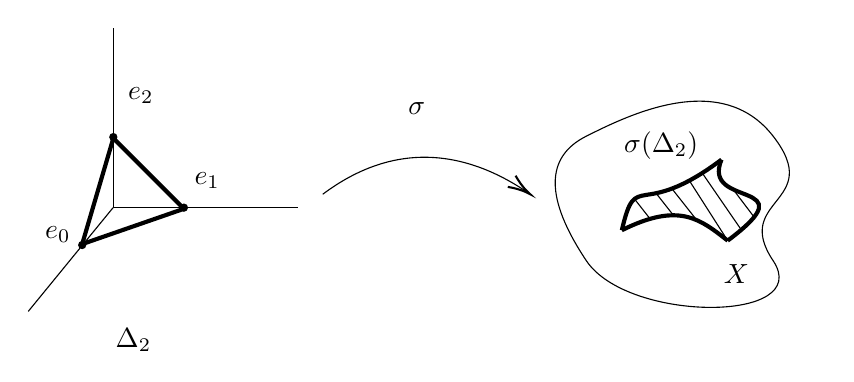
\begin{tikzpicture}[x=0.75pt,y=0.75pt,yscale=-1,xscale=1]
%uncomment if require: \path (0,512); %set diagram left start at 0, and has height of 512

%Straight Lines [id:da503174047552124] 
\draw    (109,59) -- (109,145.44) ;
%Straight Lines [id:da09475116159746144] 
\draw    (109,145.44) -- (198.11,145.44) ;
%Straight Lines [id:da7387438842628895] 
\draw    (109,145.44) -- (68.11,195.44) ;
%Shape: Free Drawing [id:dp6195845154381956] 
\draw  [line width=3] [line join = round][line cap = round] (109.11,111.44) .. controls (109.11,111.44) and (109.11,111.44) .. (109.11,111.44) ;
%Shape: Free Drawing [id:dp6516041505480692] 
\draw  [line width=3] [line join = round][line cap = round] (94.11,163.44) .. controls (94.11,163.44) and (94.11,163.44) .. (94.11,163.44) ;
%Shape: Free Drawing [id:dp5815067055358059] 
\draw  [line width=3] [line join = round][line cap = round] (143.11,145.44) .. controls (143.11,145.44) and (143.11,145.44) .. (143.11,145.44) ;
%Straight Lines [id:da01605907736149592] 
\draw [line width=1.5]    (109.11,112) -- (94.11,163) ;
%Straight Lines [id:da3089600654785245] 
\draw [line width=1.5]    (109.11,112) -- (143.11,146) ;
%Straight Lines [id:da5159186655732428] 
\draw [line width=1.5]    (94.11,163) -- (143.11,146) ;
%Shape: Polygon Curved [id:ds46177874595661206] 
\draw   (337,111) .. controls (357,101) and (401.89,78.67) .. (427,111) .. controls (452.11,143.33) and (407,141) .. (427,171) .. controls (447,201) and (357,201) .. (337,171) .. controls (317,141) and (317,121) .. (337,111) -- cycle ;
%Curve Lines [id:da493708026572965] 
\draw [line width=1.5]    (354.11,156.33) .. controls (361.11,126.33) and (362.11,152.33) .. (402.11,122.33) ;
%Curve Lines [id:da7836817972981569] 
\draw [line width=1.5]    (354.11,156.33) .. controls (382.11,142.33) and (392.11,151.33) .. (405.11,161.33) ;
%Curve Lines [id:da2253003780123357] 
\draw [line width=1.5]    (405.11,161.33) .. controls (445.11,131.33) and (392.11,146.33) .. (402.11,122.33) ;
%Straight Lines [id:da12123329661111604] 
\draw    (360,141) -- (368.11,151.33) ;
%Straight Lines [id:da001419918022801392] 
\draw    (371,139) -- (379.11,149.33) ;
%Straight Lines [id:da23513656652241943] 
\draw    (378,136) -- (390.11,151.33) ;
%Straight Lines [id:da3217109021043796] 
\draw    (387,133) -- (405.11,161.33) ;
%Straight Lines [id:da006251413827196517] 
\draw    (393,129) -- (411.11,155.33) ;
%Straight Lines [id:da5486328774853213] 
\draw    (408,137) -- (418.11,150.33) ;
%Curve Lines [id:da2653470293192983] 
\draw    (210,139) .. controls (249.2,109.6) and (284.67,121.82) .. (308.55,138) ;
\draw [shift={(310,139)}, rotate = 214.9] [color={rgb, 255:red, 0; green, 0; blue, 0 }  ][line width=0.75]    (10.93,-3.29) .. controls (6.95,-1.4) and (3.31,-0.3) .. (0,0) .. controls (3.31,0.3) and (6.95,1.4) .. (10.93,3.29)   ;

% Text Node
\draw (75,153.4) node [anchor=north west][inner sep=0.75pt]    {$e_{0}$};
% Text Node
\draw (147,127.4) node [anchor=north west][inner sep=0.75pt]    {$e_{1}$};
% Text Node
\draw (115,86.4) node [anchor=north west][inner sep=0.75pt]    {$e_{2}$};
% Text Node
\draw (109,202.4) node [anchor=north west][inner sep=0.75pt]    {$\Delta _{2}$};
% Text Node
\draw (402,171.4) node [anchor=north west][inner sep=0.75pt]    {$X$};
% Text Node
\draw (354,107.4) node [anchor=north west][inner sep=0.75pt]    {$\sigma ( \Delta _{2})$};
% Text Node
\draw (250,93.4) node [anchor=north west][inner sep=0.75pt]    {$\sigma $};


\end{tikzpicture}\]
\begin{example}
    若$C$为Euclid空间的凸集,$c_0,c_1,\cdots,c_1 \in C$,则有唯一的线性映射$\Delta_q \to C$把顶点$e_0,e_1,\cdots,e_q$分别映射为$C$中的点$c_0,c_1,\cdots,c_q$.这个映射我们记作$(c_0c_1\cdots c_q)$,
    $$
    (c_0c_1\cdots c_q) : \Delta_q \to C, \quad\sum_{i} x_i e_i \mapsto \sum_i x_i c_i
    $$
    我们把它看成是$C$上的一个$q$维奇异单形,成为\emph{线性奇异单形}.
\end{example}
\subsubsection{奇异单形的边缘算子}
首先介绍单形的边缘算子.设$e_0e_1\cdots e_i \cdots e_q$是一个$q$维定向单形,$e_0e_1\cdots \hat{e_i}\cdots e_q = e_0 e_1 \cdots e_{i-1}e_{i+1} \cdots e_q$表示从单形$e_0e_1\cdots e_i \cdots e_q$去掉顶点$e_i$后所形成的一个$q-1$维定向单形.\\
依据这一点,可以得到一个对应:
$$
(e_0,e_1,\cdots,e_{n-1}) \to e_0,e_1,\cdots e_{i-1}\hat{e}_i 
$$
对其作一个线性扩张,得到映射$\iota_i : \Delta^{q-1} \to \Delta^q$,
$$
\iota_i(t_0e_0+t_1e_1+\cdots+t_{q-1}e_{q-1}) = t_0e_0 t_1e_1+\cdots +t_{q-1}e_{q-1} +t_i e_{q+1}+ t_{q+1}e_{q+2}+\cdots +t_{q-1}e_q
$$
称为$\Delta_q$的第$i$个面(算子),这是一个嵌入映射.
\begin{example}
    考虑$\iota_i : \Delta_0 \to \Delta_1$,$i= 0,1$,容易得到.
    \[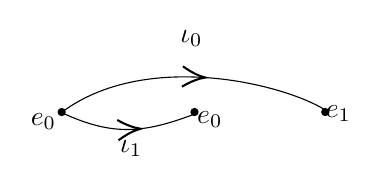
\begin{tikzpicture}[x=0.75pt,y=0.75pt,yscale=-1,xscale=1]
        %uncomment if require: \path (0,300); %set diagram left start at 0, and has height of 300
        
        %Shape: Free Drawing [id:dp7449941804994256] 
        \draw  [line width=3] [line join = round][line cap = round] (129.11,173.78) .. controls (129.11,173.78) and (129.11,173.78) .. (129.11,173.78) ;
        %Shape: Free Drawing [id:dp00985830510716168] 
        \draw  [line width=3] [line join = round][line cap = round] (193.11,173.78) .. controls (193.11,173.78) and (193.11,173.78) .. (193.11,173.78) ;
        %Curve Lines [id:da3308573165314823] 
        \draw    (129,174) .. controls (154.11,185.78) and (169.11,183.78) .. (193.11,174.78) ;
        \draw [shift={(167.11,181.82)}, rotate = 176.47] [color={rgb, 255:red, 0; green, 0; blue, 0 }  ][line width=0.75]    (10.93,-4.9) .. controls (6.95,-2.3) and (3.31,-0.67) .. (0,0) .. controls (3.31,0.67) and (6.95,2.3) .. (10.93,4.9)   ;
        %Shape: Free Drawing [id:dp88873777233093] 
        \draw  [line width=3] [line join = round][line cap = round] (256.11,173.78) .. controls (256.11,173.78) and (256.11,173.78) .. (256.11,173.78) ;
        %Curve Lines [id:da018165795265155493] 
        \draw    (129,174) .. controls (169,144) and (235.11,159.78) .. (256.11,172.78) ;
        \draw [shift={(198.23,157.16)}, rotate = 182.7] [color={rgb, 255:red, 0; green, 0; blue, 0 }  ][line width=0.75]    (10.93,-4.9) .. controls (6.95,-2.3) and (3.31,-0.67) .. (0,0) .. controls (3.31,0.67) and (6.95,2.3) .. (10.93,4.9)   ;
        
        % Text Node
        \draw (156,186.4) node [anchor=north west][inner sep=0.75pt]    {$\iota _{1}$};
        % Text Node
        \draw (185,133.4) node [anchor=north west][inner sep=0.75pt]    {$\iota _{0}$};
        % Text Node
        \draw (113,173.4) node [anchor=north west][inner sep=0.75pt]    {$e_{0}$};
        % Text Node
        \draw (193.11,172.18) node [anchor=north west][inner sep=0.75pt]    {$e_{0}$};
        % Text Node
        \draw (255.11,169.18) node [anchor=north west][inner sep=0.75pt]    {$e_{1}$};
        
        
        \end{tikzpicture}\]
        完全类似地,考察$\iota_i : \Delta_1 \to \Delta_2$,$i = 0,1,2$.容易知道
        \[\begin{tikzpicture}[x=0.75pt,y=0.75pt,yscale=-1,xscale=1]
            %uncomment if require: \path (0,300); %set diagram left start at 0, and has height of 300
            
            %Shape: Free Drawing [id:dp8830035066360153] 
            \draw  [line width=3] [line join = round][line cap = round] (203.11,190.78) .. controls (203.11,190.78) and (203.11,190.78) .. (203.11,190.78) ;
            %Shape: Free Drawing [id:dp5444529789816717] 
            \draw  [line width=3] [line join = round][line cap = round] (151.11,190.78) .. controls (151.11,190.78) and (151.11,190.78) .. (151.11,190.78) ;
            %Straight Lines [id:da550630155076905] 
            \draw    (150,191) -- (204.11,191) ;
            %Shape: Triangle [id:dp22130882389747897] 
            \draw   (383.56,155) -- (419.11,221.67) -- (348,221.67) -- cycle ;
            %Shape: Free Drawing [id:dp06193023010788212] 
            \draw  [line width=3] [line join = round][line cap = round] (383.11,153.78) .. controls (383.11,153.78) and (383.11,153.78) .. (383.11,153.78) ;
            %Shape: Free Drawing [id:dp37007755119638297] 
            \draw  [line width=3] [line join = round][line cap = round] (348.11,220.78) .. controls (348.11,220.78) and (348.11,220.78) .. (348.11,220.78) ;
            %Shape: Free Drawing [id:dp24847498796389655] 
            \draw  [line width=3] [line join = round][line cap = round] (418.11,220.78) .. controls (418.11,220.78) and (418.11,220.78) .. (418.11,220.78) ;
            %Curve Lines [id:da006029462474998359] 
            \draw    (185.24,191.2) .. controls (231.77,240.7) and (349.85,271.58) .. (382.28,225.62) ;
            \draw [shift={(383.24,224.2)}, rotate = 122.86] [color={rgb, 255:red, 0; green, 0; blue, 0 }  ][line width=0.75]    (10.93,-4.9) .. controls (6.95,-2.3) and (3.31,-0.67) .. (0,0) .. controls (3.31,0.67) and (6.95,2.3) .. (10.93,4.9)   ;
            %Curve Lines [id:da19368169284398506] 
            \draw    (177.06,191) .. controls (201.12,138.47) and (306.18,143.15) .. (365.35,187.53) ;
            \draw [shift={(366.24,188.2)}, rotate = 217.33] [color={rgb, 255:red, 0; green, 0; blue, 0 }  ][line width=0.75]    (10.93,-4.9) .. controls (6.95,-2.3) and (3.31,-0.67) .. (0,0) .. controls (3.31,0.67) and (6.95,2.3) .. (10.93,4.9)   ;
            %Curve Lines [id:da8428113189467297] 
            \draw    (176.24,183.2) .. controls (233.19,40.12) and (495.6,125.34) .. (405.62,182.35) ;
            \draw [shift={(404.24,183.2)}, rotate = 328.77] [color={rgb, 255:red, 0; green, 0; blue, 0 }  ][line width=0.75]    (10.93,-4.9) .. controls (6.95,-2.3) and (3.31,-0.67) .. (0,0) .. controls (3.31,0.67) and (6.95,2.3) .. (10.93,4.9)   ;
            
            % Text Node
            \draw (144,166.4) node [anchor=north west][inner sep=0.75pt]    {$e_{0}$};
            % Text Node
            \draw (197,166.4) node [anchor=north west][inner sep=0.75pt]    {$e_{1}$};
            % Text Node
            \draw (334,223.4) node [anchor=north west][inner sep=0.75pt]    {$e_{0}$};
            % Text Node
            \draw (421.11,225.07) node [anchor=north west][inner sep=0.75pt]    {$e_{1}$};
            % Text Node
            \draw (384,131.4) node [anchor=north west][inner sep=0.75pt]    {$e_{2}$};
            % Text Node
            \draw (278,245.4) node [anchor=north west][inner sep=0.75pt]    {$\iota _{2}$};
            % Text Node
            \draw (272,132.4) node [anchor=north west][inner sep=0.75pt]    {$\iota _{1}$};
            % Text Node
            \draw (338,85.4) node [anchor=north west][inner sep=0.75pt]    {$\iota _{0}$};
            
            
            \end{tikzpicture}\]
\end{example}
不难发现第$i$个面的定义可以自然地推广到奇异单形上.
\begin{definition}
    $X$中$q$维奇异单形的第$i$个面$\sigma_i$定义为$\sigma_i := \sigma \circ \iota_i$.
\end{definition}
奇异单形的第$i$个面有以下形象的例子($\sigma_i$)
\[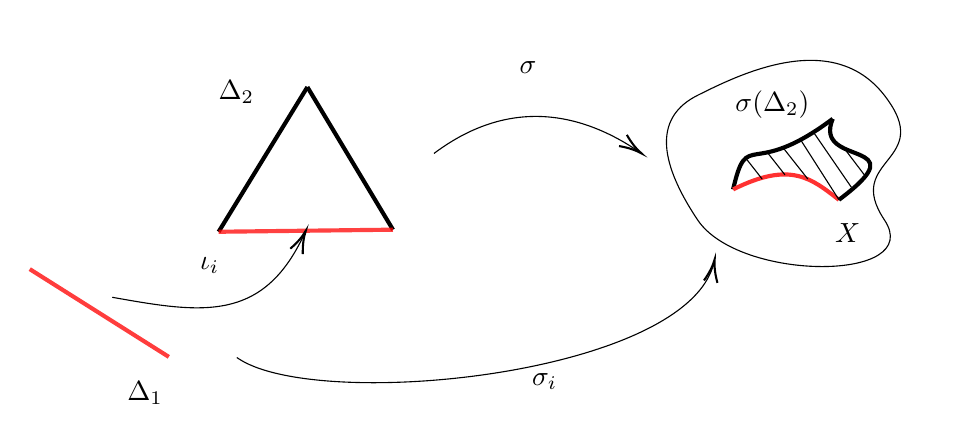
\begin{tikzpicture}[x=0.75pt,y=0.75pt,yscale=-1,xscale=1]
%uncomment if require: \path (0,300); %set diagram left start at 0, and has height of 300

%Shape: Polygon Curved [id:ds34662657022348364] 
\draw   (357,131) .. controls (377,121) and (421.89,98.67) .. (447,131) .. controls (472.11,163.33) and (427,161) .. (447,191) .. controls (467,221) and (377,221) .. (357,191) .. controls (337,161) and (337,141) .. (357,131) -- cycle ;
%Curve Lines [id:da643028031344026] 
\draw [line width=1.5]    (374.11,176.33) .. controls (381.11,146.33) and (382.11,172.33) .. (422.11,142.33) ;
%Curve Lines [id:da8982185245552112] 
\draw [color={rgb, 255:red, 255; green, 49; blue, 49 }  ,draw opacity=1 ][line width=1.5]    (374.11,176.33) .. controls (402.11,162.33) and (412.11,171.33) .. (425.11,181.33) ;
%Curve Lines [id:da5346660361158584] 
\draw [line width=1.5]    (425.11,181.33) .. controls (465.11,151.33) and (412.11,166.33) .. (422.11,142.33) ;
%Straight Lines [id:da3651154266380803] 
\draw    (380,161) -- (388.11,171.33) ;
%Straight Lines [id:da8490078509768548] 
\draw    (391,159) -- (399.11,169.33) ;
%Straight Lines [id:da1614881369599388] 
\draw    (398,156) -- (410.11,171.33) ;
%Straight Lines [id:da022264595020748068] 
\draw    (407,153) -- (425.11,181.33) ;
%Straight Lines [id:da8582309444054428] 
\draw    (413,149) -- (431.11,175.33) ;
%Straight Lines [id:da8682417870792505] 
\draw    (428,157) -- (438.11,170.33) ;
%Curve Lines [id:da172067423344767] 
\draw    (230,159) .. controls (269.2,129.6) and (304.67,141.82) .. (328.55,158) ;
\draw [shift={(330,159)}, rotate = 214.9] [color={rgb, 255:red, 0; green, 0; blue, 0 }  ][line width=0.75]    (10.93,-3.29) .. controls (6.95,-1.4) and (3.31,-0.3) .. (0,0) .. controls (3.31,0.3) and (6.95,1.4) .. (10.93,3.29)   ;
%Straight Lines [id:da010100200832178219] 
\draw [line width=1.5]    (169,127) -- (126.24,196.73) ;
%Straight Lines [id:da14966051948760328] 
\draw [line width=1.5]    (169,127) -- (210.24,195.73) ;
%Straight Lines [id:da8039502815259065] 
\draw [color={rgb, 255:red, 255; green, 5; blue, 5 }  ,draw opacity=0.76 ][line width=1.5]    (126.24,196.73) -- (210.24,195.73) ;
%Straight Lines [id:da35488428527575544] 
\draw [color={rgb, 255:red, 255; green, 0; blue, 0 }  ,draw opacity=0.76 ][line width=1.5]    (35.24,214.73) -- (102.24,257.01) ;
%Curve Lines [id:da9747852055533246] 
\draw    (75,228.3) .. controls (117.81,235.93) and (147.64,240.91) .. (167.64,197.55) ;
\draw [shift={(168.24,196.23)}, rotate = 114.06] [color={rgb, 255:red, 0; green, 0; blue, 0 }  ][line width=0.75]    (10.93,-3.29) .. controls (6.95,-1.4) and (3.31,-0.3) .. (0,0) .. controls (3.31,0.3) and (6.95,1.4) .. (10.93,3.29)   ;
%Curve Lines [id:da7560599433572159] 
\draw    (135,257.3) .. controls (171.87,283.74) and (351.59,266.37) .. (364.89,211.68) ;
\draw [shift={(365.24,210.01)}, rotate = 100.12] [color={rgb, 255:red, 0; green, 0; blue, 0 }  ][line width=0.75]    (10.93,-3.29) .. controls (6.95,-1.4) and (3.31,-0.3) .. (0,0) .. controls (3.31,0.3) and (6.95,1.4) .. (10.93,3.29)   ;

% Text Node
\draw (422,191.4) node [anchor=north west][inner sep=0.75pt]    {$X$};
% Text Node
\draw (374,127.4) node [anchor=north west][inner sep=0.75pt]    {$\sigma ( \Delta _{2})$};
% Text Node
\draw (270,113.4) node [anchor=north west][inner sep=0.75pt]    {$\sigma $};
% Text Node
\draw (81,267.7) node [anchor=north west][inner sep=0.75pt]    {$\Delta _{1}$};
% Text Node
\draw (125,122.7) node [anchor=north west][inner sep=0.75pt]    {$\Delta _{2}$};
% Text Node
\draw (116,207.7) node [anchor=north west][inner sep=0.75pt]    {$\iota _{i}$};
% Text Node
\draw (276,263.7) node [anchor=north west][inner sep=0.75pt]    {$\sigma _{i}$};


\end{tikzpicture}\]    
根据预备知识中关于单形定向的讨论,并且由$\iota_i$得知$q$维单形的边缘是$q-1$维单形,而单形又是有方向的,若一个单形两个相接面的方向相反,则必然会造成问题,因此对于一个$q$为定向单形$\Delta_q$,定义$(-1)^i \iota_i \Delta_{q-1}$为其顺向面,那么,整个定向单形的\emph{边缘}就可以表示为$\sum_{i= 0}^q (-1)^i \iota_i \Delta_{q-1}$.这自然也可以推广到奇异单形上.
\begin{definition}
    $X$中的$q$维奇异单形$\sigma : \Delta_q  \to X$的\emph{边缘},定义为$X$中的如下的$q-1$维奇异链
    $$
    \partial \sigma = \partial( \sigma \circ (e_0\cdots e_q)) := \sum_{i = 0}^q(-1)^i \sigma \circ \iota_i
    $$
\end{definition}
\begin{lemma}
    \[\begin{tikzcd}
        {\Delta_{k-2}} && {\Delta_{k-1}} \\
        \\
        {\Delta_{k-1}} && {\Delta_k}
        \arrow["{\iota_j}", from=1-1, to=1-3]
        \arrow["{\iota_i}", from=1-3, to=3-3]
        \arrow["{\iota_{i-1}}"', from=1-1, to=3-1]
        \arrow["{\iota_j}"', from=3-1, to=3-3]
    \end{tikzcd}\]
    在$1 \leq j+1 \leq i \leq k>2$时是交换的.
    \label{lem:3.2.3}
\end{lemma}
\subsubsection{奇异链复形与奇异同调群}
设$X$为拓扑空间.
\begin{definition}
    以$X$中全体$q$维奇异单形为基,生成一个自由Abel群,记作$S_q(X)$,称为$X$的$q$维\emph{奇异链群},其中的元素称为$X$的$q$维\emph{奇异链}.于是,奇异链是奇异单形的整系数线性组合:
    $$
    c_q = k_1 \sigma_q^{(1)}+\cdots + k_r\sigma_q^r. k_i \in \Z, \sigma_q^{(i)}: \Delta_q \to X
    $$
    负维数的奇异链群规定为$0$.
\end{definition}
\begin{remark}
$S_q(X)$可以被表示为$S_q(X) := \Z^{\bigoplus\Hom_{\bold{Top}}(\Delta_q, X)}$,其中对于任一集合$S$,$\Z^{\bigoplus S}: = \{\phi : S \to \Z : \text{仅对有限个}s \in S\text{有}\phi(s) \neq 0\}$.它是一个自然的阿贝尔群,通常把$\phi$写为$\sum_{s \in S}\phi(s) s$.
\end{remark}
接下来,对于奇异单形的边缘作线性扩张,得到一个\emph{边缘算子}$\partial_q : S_q(X) \to S_{q-1}(X)$,
$$
\partial_q(k_1\sigma^{(1)}_q + \cdots + k_r \sigma_q^{(r)}) := k_\partial \sigma_q^{(1)}+\cdots + k_r \partial \sigma_q^{(r)}
$$
\begin{proposition}
    两次边缘为零,即$S_*(X) = \{S_q(X),\partial_q\}$是链复形.
\end{proposition}
\begin{proof}
    代数解释:\\
    令$\sigma : \Delta_q\to X$是一个$X$中的$q$阶奇异单形,考虑
    \begin{eqnarray*}
    \partial_{k-1}\partial_k \sigma = \partial_{k-1}(\sum_{i = 0}^k (-1)^i \sigma_i) &=& \sum_{j = 0}^{k-1}(\sum_{i = 0}^k(-1)^{i+j}(\sigma_i)_j)\\ 
    &=& \sum_{k-1 \geq j \geq i \geq 0}(-1)^{i+j}\sigma \circ \iota_i \iota_j + \sum_{k \geq i \geq j-1 \geq 1}(-1)^{i+j}\sigma \iota_i \iota_j
\end{eqnarray*}
至于等式的来源可以参考下图
\[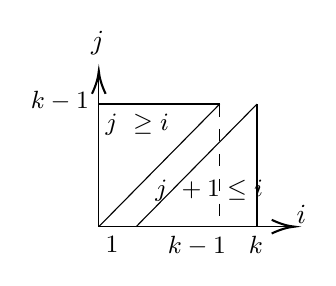
\begin{tikzpicture}[x=0.75pt,y=0.75pt,yscale=-1,xscale=1]
    %uncomment if require: \path (0,300); %set diagram left start at 0, and has height of 300
    
    %Straight Lines [id:da9048194505226212] 
    \draw    (100,110) -- (100,37.06) ;
    \draw [shift={(100,35.06)}, rotate = 90] [color={rgb, 255:red, 0; green, 0; blue, 0 }  ][line width=0.75]    (10.93,-3.29) .. controls (6.95,-1.4) and (3.31,-0.3) .. (0,0) .. controls (3.31,0.3) and (6.95,1.4) .. (10.93,3.29)   ;
    %Straight Lines [id:da8652735048806979] 
    \draw    (100,110) -- (192.24,110) ;
    \draw [shift={(194.24,110)}, rotate = 180] [color={rgb, 255:red, 0; green, 0; blue, 0 }  ][line width=0.75]    (10.93,-3.29) .. controls (6.95,-1.4) and (3.31,-0.3) .. (0,0) .. controls (3.31,0.3) and (6.95,1.4) .. (10.93,3.29)   ;
    %Straight Lines [id:da28442939191333716] 
    \draw    (100,50.93) -- (158.24,50.93) ;
    %Straight Lines [id:da664795246037033] 
    \draw    (100,110) -- (158.24,50.93) ;
    %Straight Lines [id:da12460967686209323] 
    \draw    (118,110) -- (176.24,50.93) ;
    %Straight Lines [id:da6255481967953405] 
    \draw    (176.24,50.93) -- (176.24,110.06) ;
    %Straight Lines [id:da473637212898806] 
    \draw  [dash pattern={on 4.5pt off 4.5pt}]  (158.24,50.93) -- (158.24,110.06) ;
    
    % Text Node
    \draw (95,14.4) node [anchor=north west][inner sep=0.75pt]    {$j$};
    % Text Node
    \draw (194,98.4) node [anchor=north west][inner sep=0.75pt]    {$i$};
    % Text Node
    \draw (102,113.4) node [anchor=north west][inner sep=0.75pt]  [font=\small]  {$1$};
    % Text Node
    \draw (171,113.4) node [anchor=north west][inner sep=0.75pt]  [font=\small]  {$k$};
    % Text Node
    \draw (132,113.4) node [anchor=north west][inner sep=0.75pt]  [font=\small]  {$k-1$};
    % Text Node
    \draw (66,43.4) node [anchor=north west][inner sep=0.75pt]  [font=\small]  {$k-1$};
    % Text Node
    \draw (102,54.33) node [anchor=north west][inner sep=0.75pt]  [font=\small]  {$j\ \geq i$};
    % Text Node
    \draw (126,86.4) node [anchor=north west][inner sep=0.75pt]  [font=\small]  {$j\ +1\leq i$};
    
    
    \end{tikzpicture}\]    
使用引理\ref{lem:3.2.3},将右侧$\iota_i\iota_j$转换为$\iota_{j-1}\iota_i$得到上式为$0$.\\
几何解释(自创):\\
根据单形的拆分得知,经过两次边缘映射后,其正负项相互抵消(下图是一个$\Delta_3$的例子,可以推广到奇异单形上).
\begin{figure}[h]
    \centering
    \begin{tikzpicture}[x=0.75pt,y=0.75pt,yscale=-1,xscale=1]
        %uncomment if require: \path (0,423); %set diagram left start at 0, and has height of 423
        
        %Straight Lines [id:da2683057003712348] 
        \draw    (83.11,176.78) -- (20,270) ;
        %Straight Lines [id:da9714838589404016] 
        \draw    (83.11,176.78) -- (154.11,267.78) ;
        %Straight Lines [id:da3735150508784115] 
        \draw    (20,270) -- (154.11,267.78) ;
        %Straight Lines [id:da6397676892011297] 
        \draw  [dash pattern={on 4.5pt off 4.5pt}]  (20,270) -- (81.11,242.78) ;
        %Straight Lines [id:da90634890157439] 
        \draw  [dash pattern={on 4.5pt off 4.5pt}]  (83.11,176.78) -- (81.11,242.78) ;
        %Straight Lines [id:da10319366644604022] 
        \draw  [dash pattern={on 4.5pt off 4.5pt}]  (81.11,242.78) -- (154.11,267.78) ;
        %Right Arrow [id:dp9347608471214321] 
        \draw   (165,207.47) -- (192.67,207.47) -- (192.67,202.17) -- (211.11,212.78) -- (192.67,223.39) -- (192.67,218.08) -- (165,218.08) -- cycle ;
        %Straight Lines [id:da7834820342261699] 
        \draw    (312.11,20.11) -- (276,78) ;
        \draw [shift={(290.88,54.15)}, rotate = 301.96] [color={rgb, 255:red, 0; green, 0; blue, 0 }  ][line width=0.75]    (10.93,-4.9) .. controls (6.95,-2.3) and (3.31,-0.67) .. (0,0) .. controls (3.31,0.67) and (6.95,2.3) .. (10.93,4.9)   ;
        %Straight Lines [id:da515468212229135] 
        \draw    (312.11,20.11) -- (350.11,78) ;
        \draw [shift={(327.27,43.2)}, rotate = 56.72] [color={rgb, 255:red, 0; green, 0; blue, 0 }  ][line width=0.75]    (10.93,-4.9) .. controls (6.95,-2.3) and (3.31,-0.67) .. (0,0) .. controls (3.31,0.67) and (6.95,2.3) .. (10.93,4.9)   ;
        %Straight Lines [id:da9723329548318203] 
        \draw    (276,78) -- (350.11,78) ;
        \draw [shift={(319.06,78)}, rotate = 180] [color={rgb, 255:red, 0; green, 0; blue, 0 }  ][line width=0.75]    (10.93,-4.9) .. controls (6.95,-2.3) and (3.31,-0.67) .. (0,0) .. controls (3.31,0.67) and (6.95,2.3) .. (10.93,4.9)   ;
        %Straight Lines [id:da5217347841932396] 
        \draw    (313.11,112.11) -- (277,170) ;
        \draw [shift={(298.76,135.12)}, rotate = 121.96] [color={rgb, 255:red, 0; green, 0; blue, 0 }  ][line width=0.75]    (10.93,-4.9) .. controls (6.95,-2.3) and (3.31,-0.67) .. (0,0) .. controls (3.31,0.67) and (6.95,2.3) .. (10.93,4.9)   ;
        %Straight Lines [id:da8218271470012828] 
        \draw    (313.11,112.11) -- (351.11,170) ;
        \draw [shift={(335.4,146.07)}, rotate = 236.72] [color={rgb, 255:red, 0; green, 0; blue, 0 }  ][line width=0.75]    (10.93,-4.9) .. controls (6.95,-2.3) and (3.31,-0.67) .. (0,0) .. controls (3.31,0.67) and (6.95,2.3) .. (10.93,4.9)   ;
        %Straight Lines [id:da587590665380666] 
        \draw    (277,170) -- (351.11,170) ;
        \draw [shift={(307.06,170)}, rotate = 0] [color={rgb, 255:red, 0; green, 0; blue, 0 }  ][line width=0.75]    (10.93,-4.9) .. controls (6.95,-2.3) and (3.31,-0.67) .. (0,0) .. controls (3.31,0.67) and (6.95,2.3) .. (10.93,4.9)   ;
        %Straight Lines [id:da5137587958943668] 
        \draw    (311.11,217.11) -- (275,275) ;
        \draw [shift={(289.88,251.15)}, rotate = 301.96] [color={rgb, 255:red, 0; green, 0; blue, 0 }  ][line width=0.75]    (10.93,-4.9) .. controls (6.95,-2.3) and (3.31,-0.67) .. (0,0) .. controls (3.31,0.67) and (6.95,2.3) .. (10.93,4.9)   ;
        %Straight Lines [id:da2552932766352658] 
        \draw    (311.11,217.11) -- (349.11,275) ;
        \draw [shift={(326.27,240.2)}, rotate = 56.72] [color={rgb, 255:red, 0; green, 0; blue, 0 }  ][line width=0.75]    (10.93,-4.9) .. controls (6.95,-2.3) and (3.31,-0.67) .. (0,0) .. controls (3.31,0.67) and (6.95,2.3) .. (10.93,4.9)   ;
        %Straight Lines [id:da04285724706917082] 
        \draw    (275,275) -- (349.11,275) ;
        \draw [shift={(318.06,275)}, rotate = 180] [color={rgb, 255:red, 0; green, 0; blue, 0 }  ][line width=0.75]    (10.93,-4.9) .. controls (6.95,-2.3) and (3.31,-0.67) .. (0,0) .. controls (3.31,0.67) and (6.95,2.3) .. (10.93,4.9)   ;
        %Straight Lines [id:da8416469924464907] 
        \draw    (310.11,307.11) -- (274,365) ;
        \draw [shift={(295.76,330.12)}, rotate = 121.96] [color={rgb, 255:red, 0; green, 0; blue, 0 }  ][line width=0.75]    (10.93,-4.9) .. controls (6.95,-2.3) and (3.31,-0.67) .. (0,0) .. controls (3.31,0.67) and (6.95,2.3) .. (10.93,4.9)   ;
        %Straight Lines [id:da023975347364358246] 
        \draw    (310.11,307.11) -- (348.11,365) ;
        \draw [shift={(332.4,341.07)}, rotate = 236.72] [color={rgb, 255:red, 0; green, 0; blue, 0 }  ][line width=0.75]    (10.93,-4.9) .. controls (6.95,-2.3) and (3.31,-0.67) .. (0,0) .. controls (3.31,0.67) and (6.95,2.3) .. (10.93,4.9)   ;
        %Straight Lines [id:da8170517685343011] 
        \draw    (274,365) -- (348.11,365) ;
        \draw [shift={(304.06,365)}, rotate = 0] [color={rgb, 255:red, 0; green, 0; blue, 0 }  ][line width=0.75]    (10.93,-4.9) .. controls (6.95,-2.3) and (3.31,-0.67) .. (0,0) .. controls (3.31,0.67) and (6.95,2.3) .. (10.93,4.9)   ;
        %Right Arrow [id:dp5779117078657976] 
        \draw   (384,44.33) -- (411.67,44.33) -- (411.67,40.11) -- (430.11,48.56) -- (411.67,57) -- (411.67,52.78) -- (384,52.78) -- cycle ;
        %Straight Lines [id:da4937438950315176] 
        \draw    (467,18) -- (520.11,18) ;
        \draw [shift={(499.56,18)}, rotate = 180] [color={rgb, 255:red, 0; green, 0; blue, 0 }  ][line width=0.75]    (10.93,-4.9) .. controls (6.95,-2.3) and (3.31,-0.67) .. (0,0) .. controls (3.31,0.67) and (6.95,2.3) .. (10.93,4.9)   ;
        %Straight Lines [id:da9724111287688495] 
        \draw    (468,51) -- (521.11,51) ;
        \draw [shift={(500.56,51)}, rotate = 180] [color={rgb, 255:red, 0; green, 0; blue, 0 }  ][line width=0.75]    (10.93,-4.9) .. controls (6.95,-2.3) and (3.31,-0.67) .. (0,0) .. controls (3.31,0.67) and (6.95,2.3) .. (10.93,4.9)   ;
        %Straight Lines [id:da6437597226154304] 
        \draw    (468,85) -- (521.11,85) ;
        \draw [shift={(500.56,85)}, rotate = 180] [color={rgb, 255:red, 0; green, 0; blue, 0 }  ][line width=0.75]    (10.93,-4.9) .. controls (6.95,-2.3) and (3.31,-0.67) .. (0,0) .. controls (3.31,0.67) and (6.95,2.3) .. (10.93,4.9)   ;
        %Right Arrow [id:dp9479555319764421] 
        \draw   (387,146.44) -- (414.67,146.44) -- (414.67,142.22) -- (433.11,150.67) -- (414.67,159.11) -- (414.67,154.89) -- (387,154.89) -- cycle ;
        %Straight Lines [id:da9882819810472951] 
        \draw    (468,115.11) -- (521.11,115.11) ;
        \draw [shift={(500.56,115.11)}, rotate = 180] [color={rgb, 255:red, 0; green, 0; blue, 0 }  ][line width=0.75]    (10.93,-4.9) .. controls (6.95,-2.3) and (3.31,-0.67) .. (0,0) .. controls (3.31,0.67) and (6.95,2.3) .. (10.93,4.9)   ;
        %Straight Lines [id:da26914862324305155] 
        \draw    (469,148.11) -- (522.11,148.11) ;
        \draw [shift={(501.56,148.11)}, rotate = 180] [color={rgb, 255:red, 0; green, 0; blue, 0 }  ][line width=0.75]    (10.93,-4.9) .. controls (6.95,-2.3) and (3.31,-0.67) .. (0,0) .. controls (3.31,0.67) and (6.95,2.3) .. (10.93,4.9)   ;
        %Straight Lines [id:da3230894707726426] 
        \draw    (469,182.11) -- (522.11,182.11) ;
        \draw [shift={(501.56,182.11)}, rotate = 180] [color={rgb, 255:red, 0; green, 0; blue, 0 }  ][line width=0.75]    (10.93,-4.9) .. controls (6.95,-2.3) and (3.31,-0.67) .. (0,0) .. controls (3.31,0.67) and (6.95,2.3) .. (10.93,4.9)   ;
        %Right Arrow [id:dp5885996071845241] 
        \draw   (389,247.44) -- (416.67,247.44) -- (416.67,243.22) -- (435.11,251.67) -- (416.67,260.11) -- (416.67,255.89) -- (389,255.89) -- cycle ;
        %Straight Lines [id:da3856258762242464] 
        \draw    (470,214.11) -- (523.11,214.11) ;
        \draw [shift={(502.56,214.11)}, rotate = 180] [color={rgb, 255:red, 0; green, 0; blue, 0 }  ][line width=0.75]    (10.93,-4.9) .. controls (6.95,-2.3) and (3.31,-0.67) .. (0,0) .. controls (3.31,0.67) and (6.95,2.3) .. (10.93,4.9)   ;
        %Straight Lines [id:da4365711937813117] 
        \draw    (471,247.11) -- (524.11,247.11) ;
        \draw [shift={(503.56,247.11)}, rotate = 180] [color={rgb, 255:red, 0; green, 0; blue, 0 }  ][line width=0.75]    (10.93,-4.9) .. controls (6.95,-2.3) and (3.31,-0.67) .. (0,0) .. controls (3.31,0.67) and (6.95,2.3) .. (10.93,4.9)   ;
        %Straight Lines [id:da4725915740719264] 
        \draw    (471,281.11) -- (524.11,281.11) ;
        \draw [shift={(503.56,281.11)}, rotate = 180] [color={rgb, 255:red, 0; green, 0; blue, 0 }  ][line width=0.75]    (10.93,-4.9) .. controls (6.95,-2.3) and (3.31,-0.67) .. (0,0) .. controls (3.31,0.67) and (6.95,2.3) .. (10.93,4.9)   ;
        %Right Arrow [id:dp8986328315128365] 
        \draw   (386,348.44) -- (413.67,348.44) -- (413.67,344.22) -- (432.11,352.67) -- (413.67,361.11) -- (413.67,356.89) -- (386,356.89) -- cycle ;
        %Straight Lines [id:da14695928522891766] 
        \draw    (471,320.11) -- (524.11,320.11) ;
        \draw [shift={(503.56,320.11)}, rotate = 180] [color={rgb, 255:red, 0; green, 0; blue, 0 }  ][line width=0.75]    (10.93,-4.9) .. controls (6.95,-2.3) and (3.31,-0.67) .. (0,0) .. controls (3.31,0.67) and (6.95,2.3) .. (10.93,4.9)   ;
        %Straight Lines [id:da5797605924172149] 
        \draw    (472,353.11) -- (525.11,353.11) ;
        \draw [shift={(504.56,353.11)}, rotate = 180] [color={rgb, 255:red, 0; green, 0; blue, 0 }  ][line width=0.75]    (10.93,-4.9) .. controls (6.95,-2.3) and (3.31,-0.67) .. (0,0) .. controls (3.31,0.67) and (6.95,2.3) .. (10.93,4.9)   ;
        %Straight Lines [id:da8088231678038875] 
        \draw    (472,387.11) -- (525.11,387.11) ;
        \draw [shift={(504.56,387.11)}, rotate = 180] [color={rgb, 255:red, 0; green, 0; blue, 0 }  ][line width=0.75]    (10.93,-4.9) .. controls (6.95,-2.3) and (3.31,-0.67) .. (0,0) .. controls (3.31,0.67) and (6.95,2.3) .. (10.93,4.9)   ;
        %Shape: Rectangle [id:dp06614670898470587] 
        \draw   (234.38,6.11) -- (376.18,6.11) -- (376.18,391.66) -- (234.38,391.66) -- cycle ;
        %Straight Lines [id:da3327587478277738] 
        \draw    (235.31,97.11) -- (307.26,97.11) -- (377.11,97.11) ;
        %Straight Lines [id:da45915359952520385] 
        \draw    (235.31,196.78) -- (377.11,196.78) ;
        %Straight Lines [id:da165433183849641] 
        \draw    (234.38,295.11) -- (376.18,295.11) ;
        
        % Text Node
        \draw (78,147.4) node [anchor=north west][inner sep=0.75pt]    {$e_{0}$};
        % Text Node
        \draw (12,274.4) node [anchor=north west][inner sep=0.75pt]    {$e_{1}$};
        % Text Node
        \draw (148,270.4) node [anchor=north west][inner sep=0.75pt]    {$e_{2}$};
        % Text Node
        \draw (87,222.4) node [anchor=north west][inner sep=0.75pt]    {$e_{3}$};
        % Text Node
        \draw (75,292.4) node [anchor=north west][inner sep=0.75pt]    {$\Delta _{3}$};
        % Text Node
        \draw (240,46.4) node [anchor=north west][inner sep=0.75pt]    {$0:$};
        % Text Node
        \draw (305,9.4) node [anchor=north west][inner sep=0.75pt]    {$e_{1}$};
        % Text Node
        \draw (262,77.4) node [anchor=north west][inner sep=0.75pt]    {$e_{2}$};
        % Text Node
        \draw (350.11,76.4) node [anchor=north west][inner sep=0.75pt]    {$e_{3}$};
        % Text Node
        \draw (307.11,101.51) node [anchor=north west][inner sep=0.75pt]    {$e_{0}$};
        % Text Node
        \draw (261,172.4) node [anchor=north west][inner sep=0.75pt]    {$e_{2}$};
        % Text Node
        \draw (353.11,173.4) node [anchor=north west][inner sep=0.75pt]    {$e_{3}$};
        % Text Node
        \draw (241,237.4) node [anchor=north west][inner sep=0.75pt]    {$2:$};
        % Text Node
        \draw (305.11,205.18) node [anchor=north west][inner sep=0.75pt]    {$e_{0}$};
        % Text Node
        \draw (260,272.4) node [anchor=north west][inner sep=0.75pt]    {$e_{1}$};
        % Text Node
        \draw (351.11,271.4) node [anchor=north west][inner sep=0.75pt]    {$e_{3}$};
        % Text Node
        \draw (241,328.4) node [anchor=north west][inner sep=0.75pt]    {$3:$};
        % Text Node
        \draw (303,298.4) node [anchor=north west][inner sep=0.75pt]    {$e_{0}$};
        % Text Node
        \draw (258,367.4) node [anchor=north west][inner sep=0.75pt]    {$e_{1}$};
        % Text Node
        \draw (350.11,368.4) node [anchor=north west][inner sep=0.75pt]    {$e_{2}$};
        % Text Node
        \draw (176,185.4) node [anchor=north west][inner sep=0.75pt]    {$\partial $};
        % Text Node
        \draw (396,24.4) node [anchor=north west][inner sep=0.75pt]    {$\partial $};
        % Text Node
        \draw (239,137.4) node [anchor=north west][inner sep=0.75pt]    {$1:$};
        % Text Node
        \draw (446,7.4) node [anchor=north west][inner sep=0.75pt]    {$e_{1}$};
        % Text Node
        \draw (529,10.4) node [anchor=north west][inner sep=0.75pt]    {$e_{2}$};
        % Text Node
        \draw (447,40.4) node [anchor=north west][inner sep=0.75pt]    {$e_{2}$};
        % Text Node
        \draw (532,41.4) node [anchor=north west][inner sep=0.75pt]    {$e_{3}$};
        % Text Node
        \draw (447,74.4) node [anchor=north west][inner sep=0.75pt]    {$e_{3}$};
        % Text Node
        \draw (530,76.4) node [anchor=north west][inner sep=0.75pt]    {$e_{1}$};
        % Text Node
        \draw (399,126.51) node [anchor=north west][inner sep=0.75pt]    {$\partial $};
        % Text Node
        \draw (447,104.51) node [anchor=north west][inner sep=0.75pt]    {$e_{0}$};
        % Text Node
        \draw (532,105.51) node [anchor=north west][inner sep=0.75pt]    {$e_{3}$};
        % Text Node
        \draw (448,137.51) node [anchor=north west][inner sep=0.75pt]    {$e_{2}$};
        % Text Node
        \draw (531,138.51) node [anchor=north west][inner sep=0.75pt]    {$e_{0}$};
        % Text Node
        \draw (448,171.51) node [anchor=north west][inner sep=0.75pt]    {$e_{3}$};
        % Text Node
        \draw (531,172.51) node [anchor=north west][inner sep=0.75pt]    {$e_{2}$};
        % Text Node
        \draw (401,227.51) node [anchor=north west][inner sep=0.75pt]    {$\partial $};
        % Text Node
        \draw (449,203.51) node [anchor=north west][inner sep=0.75pt]    {$e_{0}$};
        % Text Node
        \draw (532,204.51) node [anchor=north west][inner sep=0.75pt]    {$e_{1}$};
        % Text Node
        \draw (450,236.51) node [anchor=north west][inner sep=0.75pt]    {$e_{1}$};
        % Text Node
        \draw (533,237.51) node [anchor=north west][inner sep=0.75pt]    {$e_{3}$};
        % Text Node
        \draw (450,270.51) node [anchor=north west][inner sep=0.75pt]    {$e_{3}$};
        % Text Node
        \draw (533,271.51) node [anchor=north west][inner sep=0.75pt]    {$e_{0}$};
        % Text Node
        \draw (398,328.51) node [anchor=north west][inner sep=0.75pt]    {$\partial $};
        % Text Node
        \draw (450,308.51) node [anchor=north west][inner sep=0.75pt]    {$e_{1}$};
        % Text Node
        \draw (533,310.51) node [anchor=north west][inner sep=0.75pt]    {$e_{0}$};
        % Text Node
        \draw (451,342.51) node [anchor=north west][inner sep=0.75pt]    {$e_{0}$};
        % Text Node
        \draw (534,343.51) node [anchor=north west][inner sep=0.75pt]    {$e_{2}$};
        % Text Node
        \draw (451,376.51) node [anchor=north west][inner sep=0.75pt]    {$e_{2}$};
        % Text Node
        \draw (534,377.51) node [anchor=north west][inner sep=0.75pt]    {$e_{1}$};
        % Text Node
        \draw (556,187.4) node [anchor=north west][inner sep=0.75pt]  [font=\LARGE]  {$=0$};
        
        
        \end{tikzpicture}
\end{figure}
不难发现对于所有的奇异单形,在计算其两次边缘后,由于方向互相抵消,因此最终结果为$0$.
\end{proof}
\begin{definition}
    链复形$S_*(X) = \{S_q(X),\partial_q\}$称为$X$的\emph{奇异链复形}.链复形$S_*(X)$的同调群称为$X$的\emph{奇异同调群},记作
    $$
    H_*(X) := H_*(S_*(X))
    $$
\end{definition}
空间$X$的奇异闭链,奇异边缘链,奇异同调类等等,就是指链复形$S_*(X)$中的闭链,边缘链,同调类等等.
\begin{definition}
    设$f : X \to Y$是映射.它把$X$的每个奇异单形$\sigma :\Delta_q \to X$映射为$Y$的一个奇异单形
    $$
    f_{\#} := f \circ \sigma
    $$
    通过线性扩张,我们得到了同态$f_{\#} : S_*(X) \to S_*(Y)$.
\end{definition}
\newpage
\subsection{The sigular homology of a star-shaped set in $\R^n$}
这是一个超级简单的计算奇异同调群的例子:
\begin{definition}
    Let $0 \in X \subset \R^n$, such that $t \cdot P \in X$ if $t \in [0,1]$,$P \in X$. Then say $X$ is a star-shaped set.
\end{definition}
\begin{example}
    A star-shaped set $X$ as shown in the figure below
   \[\begin{tikzpicture}[x=0.75pt,y=0.75pt,yscale=-1,xscale=1]
        %uncomment if require: \path (0,300); %set diagram left start at 0, and has height of 300
        
        %Shape: Polygon Curved [id:ds8577046931655508] 
        \draw   (140,70) .. controls (160,60) and (283,30) .. (318.24,56.79) .. controls (353.48,83.57) and (290.48,137.57) .. (273.24,152.79) .. controls (256,168) and (160,160) .. (140,130) .. controls (120,100) and (120,80) .. (140,70) -- cycle ;
        %Shape: Free Drawing [id:dp25267980618306396] 
        \draw  [line width=3] [line join = round][line cap = round] (202.24,96.79) .. controls (202.24,96.79) and (202.24,96.79) .. (202.24,96.79) ;
        %Shape: Free Drawing [id:dp22361539780001993] 
        \draw  [line width=3] [line join = round][line cap = round] (281.24,86.79) .. controls (281.24,86.79) and (281.24,86.79) .. (281.24,86.79) ;
        %Straight Lines [id:da47125633247908283] 
        \draw    (202.24,96.79) -- (282.24,86.79) ;
        %Shape: Free Drawing [id:dp22519794442687346] 
        \draw  [line width=3] [line join = round][line cap = round] (233.24,92.79) .. controls (233.24,92.79) and (233.24,92.79) .. (233.24,92.79) ;
        
        % Text Node
        \draw (186,112.4) node [anchor=north west][inner sep=0.75pt]    {$O$};
        % Text Node
        \draw (281,98.4) node [anchor=north west][inner sep=0.75pt]    {$P$};
        % Text Node
        \draw (132,72.4) node [anchor=north west][inner sep=0.75pt]    {$X$};
        % Text Node
        \draw (225,102.4) node [anchor=north west][inner sep=0.75pt]    {$t\cdotp P$};
        
        
        \end{tikzpicture}\]
\end{example}
(由于英文不好,后半段使用中文讲解)\\
考虑一个星型的拓扑空间$X$,我们现在想求出它的奇异同调群$H_\cdot(X)$,先观察一个最简单的例子,在$\R^2$上的一个拓扑空间$X$
\[\begin{tikzpicture}[x=0.75pt,y=0.75pt,yscale=-1,xscale=1]
    %uncomment if require: \path (0,300); %set diagram left start at 0, and has height of 300
    
    %Shape: Polygon Curved [id:ds5411478507797027] 
    \draw   (134.24,73.03) .. controls (151.48,53.46) and (172.39,93.98) .. (205.24,94.03) .. controls (238.08,94.08) and (278.24,58.03) .. (271.24,78.32) .. controls (264.24,98.6) and (326,175.6) .. (308.24,208.03) .. controls (290.48,240.46) and (160,225.6) .. (140,195.6) .. controls (120,165.6) and (117,92.6) .. (134.24,73.03) -- cycle ;
    
    % Text Node
    \draw (205,61.4) node [anchor=north west][inner sep=0.75pt]    {$X$};
    
    
    \end{tikzpicture}\]
    现在计算其一维同调群$H_1(X) = Z_1(X)/B_1(X)$,即
    \[\begin{tikzcd}
        {S_2(X)} && {S_1(X)} && {S_0(X)}
        \arrow["{\partial_2}", from=1-1, to=1-3]
        \arrow["{\partial_1}", from=1-3, to=1-5]
    \end{tikzcd}\]
    上链中的$\ker \partial_1 / \Image \partial_2$.\\
    不难发现,$S_1(X)$中的元素可以被拆成一些路径的线性组合
    \[\begin{tikzpicture}[x=0.75pt,y=0.75pt,yscale=-1,xscale=1]
        %uncomment if require: \path (0,300); %set diagram left start at 0, and has height of 300
        
        %Straight Lines [id:da42658851987113744] 
        \draw    (120,252) -- (120,170.54) ;
        \draw [shift={(120,168.54)}, rotate = 90] [color={rgb, 255:red, 0; green, 0; blue, 0 }  ][line width=0.75]    (10.93,-3.29) .. controls (6.95,-1.4) and (3.31,-0.3) .. (0,0) .. controls (3.31,0.3) and (6.95,1.4) .. (10.93,3.29)   ;
        %Straight Lines [id:da1546809730437031] 
        \draw    (120,252) -- (209.24,252) ;
        \draw [shift={(211.24,252)}, rotate = 180] [color={rgb, 255:red, 0; green, 0; blue, 0 }  ][line width=0.75]    (10.93,-3.29) .. controls (6.95,-1.4) and (3.31,-0.3) .. (0,0) .. controls (3.31,0.3) and (6.95,1.4) .. (10.93,3.29)   ;
        %Straight Lines [id:da8577607803360965] 
        \draw    (120,210.27) -- (165.62,252) ;
        %Shape: Polygon Curved [id:ds13829699022922015] 
        \draw   (350.01,153.96) .. controls (363.85,137.28) and (380.63,171.81) .. (406.99,171.86) .. controls (433.35,171.9) and (465.58,141.17) .. (459.96,158.46) .. controls (454.34,175.75) and (503.91,241.38) .. (489.65,269.02) .. controls (475.4,296.66) and (370.69,284) .. (354.64,258.43) .. controls (338.58,232.86) and (336.18,170.64) .. (350.01,153.96) -- cycle ;
        %Curve Lines [id:da9426814463681075] 
        \draw    (389.14,248.45) .. controls (389.34,223.48) and (434.28,235.42) .. (432.67,207.29) ;
        %Curve Lines [id:da18986759721600577] 
        \draw    (224,204.89) .. controls (263.6,175.19) and (282.85,174.61) .. (322.78,203.99) ;
        \draw [shift={(324,204.89)}, rotate = 216.61] [color={rgb, 255:red, 0; green, 0; blue, 0 }  ][line width=0.75]    (10.93,-4.9) .. controls (6.95,-2.3) and (3.31,-0.67) .. (0,0) .. controls (3.31,0.67) and (6.95,2.3) .. (10.93,4.9)   ;
        %Shape: Free Drawing [id:dp4493198739202313] 
        \draw  [line width=3] [line join = round][line cap = round] (120.24,210.6) .. controls (120.24,210.6) and (120.24,210.6) .. (120.24,210.6) ;
        %Shape: Free Drawing [id:dp6287139462681155] 
        \draw  [color={rgb, 255:red, 245; green, 166; blue, 35 }  ,draw opacity=1 ][line width=3] [line join = round][line cap = round] (389.24,248.6) .. controls (389.24,248.6) and (389.24,248.6) .. (389.24,248.6) ;
        %Shape: Free Drawing [id:dp25869264906838096] 
        \draw  [line width=3] [line join = round][line cap = round] (433.24,206.6) .. controls (433.24,206.6) and (433.24,206.6) .. (433.24,206.6) ;
        %Shape: Free Drawing [id:dp8029651352026388] 
        \draw  [color={rgb, 255:red, 245; green, 166; blue, 35 }  ,draw opacity=1 ][line width=3] [line join = round][line cap = round] (165.24,252.6) .. controls (165.24,252.6) and (165.24,252.6) .. (165.24,252.6) ;
        
        % Text Node
        \draw (97,254.4) node [anchor=north west][inner sep=0.75pt]    {$0$};
        % Text Node
        \draw (102,200.4) node [anchor=north west][inner sep=0.75pt]    {$1$};
        % Text Node
        \draw (159,258.43) node [anchor=north west][inner sep=0.75pt]    {$1$};
        % Text Node
        \draw (156,200.43) node [anchor=north west][inner sep=0.75pt]    {$\Delta _{1}$};
        % Text Node
        \draw (388.42,172.92) node [anchor=north west][inner sep=0.75pt]    {$X$};
        % Text Node
        \draw (267,151.29) node [anchor=north west][inner sep=0.75pt]    {$\sigma $};
        % Text Node
        \draw (427,184.29) node [anchor=north west][inner sep=0.75pt]    {$+$};
        % Text Node
        \draw (383,252.29) node [anchor=north west][inner sep=0.75pt]    {$-$};
        % Text Node
        \draw (213.24,255.4) node [anchor=north west][inner sep=0.75pt]    {$e_{0}$};
        % Text Node
        \draw (106,148.29) node [anchor=north west][inner sep=0.75pt]    {$e_{1}$};
        
        
        \end{tikzpicture}\]
        而其边界就是取该路径的两个端点并赋予正负号.\\
        因此$X$中的闭曲线(方向不固定),可以再把它细分为一些路径的并,只要确定了合适的方向,就可以将其边界(指路径的)转化为$0$.而后将其分解为若干个二维奇异单形的并
        \[\begin{tikzpicture}[x=0.75pt,y=0.75pt,yscale=-1,xscale=1]
            %uncomment if require: \path (0,300); %set diagram left start at 0, and has height of 300
            
            %Straight Lines [id:da7371590459656794] 
            \draw    (216.24,155.22) -- (262.24,144.84) ;
            %Straight Lines [id:da8251636480249205] 
            \draw    (216.24,155.22) -- (260.24,193.13) ;
            %Straight Lines [id:da09124276797330722] 
            \draw    (175,131) -- (216.24,155.22) ;
            %Straight Lines [id:da642199634802505] 
            \draw    (216.24,155.22) -- (207.24,203.13) ;
            %Shape: Polygon Curved [id:ds5411478507797027] 
            \draw   (134.24,73.03) .. controls (151.48,53.46) and (172.39,93.98) .. (205.24,94.03) .. controls (238.08,94.08) and (278.24,58.03) .. (271.24,78.32) .. controls (264.24,98.6) and (326,175.6) .. (308.24,208.03) .. controls (290.48,240.46) and (160,225.6) .. (140,195.6) .. controls (120,165.6) and (117,92.6) .. (134.24,73.03) -- cycle ;
            %Shape: Free Drawing [id:dp17142687304476456] 
            \draw  [line width=3] [line join = round][line cap = round] (216.24,155.03) .. controls (216.24,155.03) and (216.24,155.03) .. (216.24,155.03) ;
            %Curve Lines [id:da18814132228723213] 
            \draw    (175,131) .. controls (215,101) and (247.48,110.68) .. (262.24,144.84) ;
            \draw [shift={(216.78,113.15)}, rotate = 359.96] [color={rgb, 255:red, 0; green, 0; blue, 0 }  ][line width=0.75]    (10.93,-4.9) .. controls (6.95,-2.3) and (3.31,-0.67) .. (0,0) .. controls (3.31,0.67) and (6.95,2.3) .. (10.93,4.9)   ;
            %Curve Lines [id:da48941886576983706] 
            \draw    (262.24,144.84) .. controls (250.24,160.13) and (248.24,180.13) .. (260.24,193.13) ;
            \draw [shift={(253.48,162.12)}, rotate = 100.5] [color={rgb, 255:red, 0; green, 0; blue, 0 }  ][line width=0.75]    (10.93,-4.9) .. controls (6.95,-2.3) and (3.31,-0.67) .. (0,0) .. controls (3.31,0.67) and (6.95,2.3) .. (10.93,4.9)   ;
            %Curve Lines [id:da9033137518808732] 
            \draw    (175,131) .. controls (146.24,143.13) and (157.24,161.22) .. (166.24,177.22) .. controls (175.24,193.22) and (210.24,183.13) .. (207.24,203.13) ;
            %Curve Lines [id:da354703034403139] 
            \draw    (207.24,203.13) .. controls (240.24,200.13) and (241.24,224.13) .. (260.24,193.13) ;
            \draw [shift={(243.07,209.17)}, rotate = 190.43] [color={rgb, 255:red, 0; green, 0; blue, 0 }  ][line width=0.75]    (10.93,-4.9) .. controls (6.95,-2.3) and (3.31,-0.67) .. (0,0) .. controls (3.31,0.67) and (6.95,2.3) .. (10.93,4.9)   ;
            %Shape: Free Drawing [id:dp11774394185971992] 
            \draw  [line width=3] [line join = round][line cap = round] (263.24,145.03) .. controls (263.24,145.03) and (263.24,145.03) .. (263.24,145.03) ;
            %Shape: Free Drawing [id:dp8195311437658195] 
            \draw  [line width=3] [line join = round][line cap = round] (175.24,131.03) .. controls (175.24,131.03) and (175.24,131.03) .. (175.24,131.03) ;
            %Shape: Free Drawing [id:dp187390093599622] 
            \draw  [line width=3] [line join = round][line cap = round] (207.24,203.03) .. controls (207.24,203.03) and (207.24,203.03) .. (207.24,203.03) ;
            %Shape: Free Drawing [id:dp382936273503953] 
            \draw  [line width=3] [line join = round][line cap = round] (260.24,192.03) .. controls (260.24,192.03) and (260.24,192.03) .. (260.24,192.03) ;
            \draw   (167.16,167.93) .. controls (166.89,173.42) and (167.75,177.98) .. (169.75,181.63) .. controls (166.61,178.89) and (162.34,177.08) .. (156.92,176.17) ;
            
            % Text Node
            \draw (205,61.4) node [anchor=north west][inner sep=0.75pt]    {$X$};
            % Text Node
            \draw (209,165.4) node [anchor=north west][inner sep=0.75pt]    {$O$};
            % Text Node
            \draw (269,161.4) node [anchor=north west][inner sep=0.75pt]    {$\sigma $};
            % Text Node
            \draw (249,104.4) node [anchor=north west][inner sep=0.75pt]    {$\sigma '$};
            % Text Node
            \draw (147,182.4) node [anchor=north west][inner sep=0.75pt]    {$\sigma ''$};
            % Text Node
            \draw (236,208.4) node [anchor=north west][inner sep=0.75pt]    {$\sigma '''$};
            
            
            \end{tikzpicture}\]           
            接下来说明通过这种方式可以得到$H_k(X) = 0,k >0$.
            \begin{proof}
                以$\Delta_1$为例,映射$\sigma$将$\Delta_1$映射为$X$上的道路.接下来我们想要将一个二维单形$\Delta_2$也映射到拓扑空间$X$上,并且使得$\sigma(\Delta_1)$为其$t_0$面.如图所示
                \[\begin{tikzpicture}[x=0.75pt,y=0.75pt,yscale=-1,xscale=1]
                    %uncomment if require: \path (0,363); %set diagram left start at 0, and has height of 363
                    
                    %Straight Lines [id:da9334478549442882] 
                    \draw [color={rgb, 255:red, 139; green, 87; blue, 42 }  ,draw opacity=1 ]   (120.11,313.31) -- (172.11,275.09) ;
                    %Straight Lines [id:da29835315827904574] 
                    \draw [color={rgb, 255:red, 139; green, 87; blue, 42 }  ,draw opacity=1 ]   (409.11,142.42) -- (477.11,120.09) ;
                    %Straight Lines [id:da4310757431738286] 
                    \draw    (140,160.39) -- (140,78.94) ;
                    \draw [shift={(140,76.94)}, rotate = 90] [color={rgb, 255:red, 0; green, 0; blue, 0 }  ][line width=0.75]    (10.93,-3.29) .. controls (6.95,-1.4) and (3.31,-0.3) .. (0,0) .. controls (3.31,0.3) and (6.95,1.4) .. (10.93,3.29)   ;
                    %Straight Lines [id:da24987023174283696] 
                    \draw    (140,160.39) -- (229.24,160.39) ;
                    \draw [shift={(231.24,160.39)}, rotate = 180] [color={rgb, 255:red, 0; green, 0; blue, 0 }  ][line width=0.75]    (10.93,-3.29) .. controls (6.95,-1.4) and (3.31,-0.3) .. (0,0) .. controls (3.31,0.3) and (6.95,1.4) .. (10.93,3.29)   ;
                    %Straight Lines [id:da4848246787165955] 
                    \draw [color={rgb, 255:red, 245; green, 166; blue, 35 }  ,draw opacity=1 ]   (140,118.66) -- (185.62,160.39) ;
                    %Curve Lines [id:da49187734630239577] 
                    \draw [color={rgb, 255:red, 245; green, 166; blue, 35 }  ,draw opacity=1 ]   (244,113.28) .. controls (283.6,83.58) and (302.85,83) .. (342.78,112.38) ;
                    \draw [shift={(344,113.28)}, rotate = 216.61] [color={rgb, 255:red, 245; green, 166; blue, 35 }  ,draw opacity=1 ][line width=0.75]    (10.93,-4.9) .. controls (6.95,-2.3) and (3.31,-0.67) .. (0,0) .. controls (3.31,0.67) and (6.95,2.3) .. (10.93,4.9)   ;
                    %Shape: Free Drawing [id:dp5464440522353111] 
                    \draw  [line width=3] [line join = round][line cap = round] (410.11,141.98) .. controls (410.11,141.98) and (410.11,141.98) .. (410.11,141.98) ;
                    %Curve Lines [id:da7697452573180901] 
                    \draw [color={rgb, 255:red, 245; green, 166; blue, 35 }  ,draw opacity=1 ]   (501.11,151.65) .. controls (458.11,117.65) and (487.11,81.65) .. (430.11,55.65) ;
                    \draw [shift={(468.5,93.78)}, rotate = 70.71] [color={rgb, 255:red, 245; green, 166; blue, 35 }  ,draw opacity=1 ][line width=0.75]    (10.93,-4.9) .. controls (6.95,-2.3) and (3.31,-0.67) .. (0,0) .. controls (3.31,0.67) and (6.95,2.3) .. (10.93,4.9)   ;
                    %Straight Lines [id:da3315852378526212] 
                    \draw    (145,333.31) -- (145,208.94) ;
                    \draw [shift={(145,206.94)}, rotate = 90] [color={rgb, 255:red, 0; green, 0; blue, 0 }  ][line width=0.75]    (10.93,-3.29) .. controls (6.95,-1.4) and (3.31,-0.3) .. (0,0) .. controls (3.31,0.3) and (6.95,1.4) .. (10.93,3.29)   ;
                    %Straight Lines [id:da1999782877563221] 
                    \draw    (105.11,291.39) -- (234.24,291.39) ;
                    \draw [shift={(236.24,291.39)}, rotate = 180] [color={rgb, 255:red, 0; green, 0; blue, 0 }  ][line width=0.75]    (10.93,-3.29) .. controls (6.95,-1.4) and (3.31,-0.3) .. (0,0) .. controls (3.31,0.3) and (6.95,1.4) .. (10.93,3.29)   ;
                    %Straight Lines [id:da08203213793466624] 
                    \draw [color={rgb, 255:red, 245; green, 166; blue, 35 }  ,draw opacity=1 ]   (145,249.66) -- (190.62,291.39) ;
                    %Straight Lines [id:da7392114526593221] 
                    \draw    (178.11,262.65) -- (89.62,339.34) ;
                    \draw [shift={(88.11,340.65)}, rotate = 319.09] [color={rgb, 255:red, 0; green, 0; blue, 0 }  ][line width=0.75]    (10.93,-3.29) .. controls (6.95,-1.4) and (3.31,-0.3) .. (0,0) .. controls (3.31,0.3) and (6.95,1.4) .. (10.93,3.29)   ;
                    %Straight Lines [id:da4501143949572324] 
                    \draw    (145,249.66) -- (120.11,313.31) ;
                    %Straight Lines [id:da4592030843775976] 
                    \draw    (120.11,313.31) -- (190.62,291.39) ;
                    %Curve Lines [id:da5813069734689664] 
                    \draw    (311,276.42) .. controls (345.76,298.53) and (398.05,258.57) .. (398.12,208.28) ;
                    \draw [shift={(398.11,206.76)}, rotate = 88.88] [color={rgb, 255:red, 0; green, 0; blue, 0 }  ][line width=0.75]    (10.93,-3.29) .. controls (6.95,-1.4) and (3.31,-0.3) .. (0,0) .. controls (3.31,0.3) and (6.95,1.4) .. (10.93,3.29)   ;
                    %Straight Lines [id:da6150148795445465] 
                    \draw    (430.11,55.65) -- (409.11,142.42) ;
                    %Straight Lines [id:da12807809549128657] 
                    \draw    (409.11,142.42) -- (501.11,151.65) ;
                    %Curve Lines [id:da3739297113453761] 
                    \draw    (162,283) .. controls (166.07,308.83) and (167.09,373.77) .. (205.92,345.96) ;
                    \draw [shift={(207.11,345.09)}, rotate = 143.13] [color={rgb, 255:red, 0; green, 0; blue, 0 }  ][line width=0.75]    (10.93,-3.29) .. controls (6.95,-1.4) and (3.31,-0.3) .. (0,0) .. controls (3.31,0.3) and (6.95,1.4) .. (10.93,3.29)   ;
                    %Shape: Free Drawing [id:dp3592609077439066] 
                    \draw  [color={rgb, 255:red, 245; green, 166; blue, 35 }  ,draw opacity=1 ][line width=3] [line join = round][line cap = round] (477.24,119.98) .. controls (477.24,119.98) and (477.24,119.98) .. (477.24,119.98) ;
                    %Shape: Free Drawing [id:dp3979223938444696] 
                    \draw  [color={rgb, 255:red, 245; green, 166; blue, 35 }  ,draw opacity=1 ][line width=3] [line join = round][line cap = round] (172.24,274.6) .. controls (172.24,274.6) and (172.24,274.6) .. (172.24,274.6) ;
                    %Shape: Free Drawing [id:dp50700383106198] 
                    \draw  [color={rgb, 255:red, 139; green, 87; blue, 42 }  ,draw opacity=1 ][line width=3] [line join = round][line cap = round] (461.24,125.6) .. controls (461.24,125.6) and (461.24,125.6) .. (461.24,125.6) ;
                    %Shape: Free Drawing [id:dp3644883341706704] 
                    \draw  [color={rgb, 255:red, 139; green, 87; blue, 42 }  ,draw opacity=1 ][line width=3] [line join = round][line cap = round] (162.24,282.6) .. controls (162.24,282.6) and (162.24,282.6) .. (162.24,282.6) ;
                    %Curve Lines [id:da9305951587226238] 
                    \draw    (172.11,275.09) .. controls (213.82,289.64) and (224.48,266.55) .. (226,245.99) ;
                    \draw [shift={(226.11,244.09)}, rotate = 92.73] [color={rgb, 255:red, 0; green, 0; blue, 0 }  ][line width=0.75]    (10.93,-3.29) .. controls (6.95,-1.4) and (3.31,-0.3) .. (0,0) .. controls (3.31,0.3) and (6.95,1.4) .. (10.93,3.29)   ;
                    %Curve Lines [id:da38170185179585125] 
                    \draw    (461,125) .. controls (467.02,154.64) and (476.81,132.77) .. (478.06,175.11) ;
                    \draw [shift={(478.11,177.09)}, rotate = 268.73] [color={rgb, 255:red, 0; green, 0; blue, 0 }  ][line width=0.75]    (10.93,-3.29) .. controls (6.95,-1.4) and (3.31,-0.3) .. (0,0) .. controls (3.31,0.3) and (6.95,1.4) .. (10.93,3.29)   ;
                    
                    % Text Node
                    \draw (176,108.82) node [anchor=north west][inner sep=0.75pt]    {$\Delta _{1}$};
                    % Text Node
                    \draw (233.24,163.79) node [anchor=north west][inner sep=0.75pt]    {$t_{0}$};
                    % Text Node
                    \draw (126,56.68) node [anchor=north west][inner sep=0.75pt]    {$t_{1}$};
                    % Text Node
                    \draw (114,247.82) node [anchor=north west][inner sep=0.75pt]    {$\Delta _{2}$};
                    % Text Node
                    \draw (129,189.68) node [anchor=north west][inner sep=0.75pt]    {$t_{1}$};
                    % Text Node
                    \draw (81.24,311.79) node [anchor=north west][inner sep=0.75pt]    {$t_{0}$};
                    % Text Node
                    \draw (238,283.05) node [anchor=north west][inner sep=0.75pt]    {$t_{2}$};
                    % Text Node
                    \draw (395,144.4) node [anchor=north west][inner sep=0.75pt]    {$O$};
                    % Text Node
                    \draw (529,33.4) node [anchor=north west][inner sep=0.75pt]    {$\subset \mathbb{R}^{n}$};
                    % Text Node
                    \draw (191,323.4) node [anchor=north west][inner sep=0.75pt]    {$( t_{0} ,t_{1} ,t_{2})$};
                    % Text Node
                    \draw (181,212.4) node [anchor=north west][inner sep=0.75pt]    {$\left( 0,\frac{t_{1}}{t_{1} +t_{2}} ,\frac{t_{2}}{t_{1} +t_{2}}\right)$};
                    % Text Node
                    \draw (287,66.4) node [anchor=north west][inner sep=0.75pt]    {$\sigma $};
                    % Text Node
                    \draw (472,84.4) node [anchor=north west][inner sep=0.75pt]    {$\sigma \left(\frac{t_{1}}{t_{1} +t_{2}} ,\frac{t_{2}}{t_{1} +t_{2}}\right)$};
                    % Text Node
                    \draw (434,172.4) node [anchor=north west][inner sep=0.75pt]    {$( 1-t_{0}) \sigma \left(\frac{t_{1}}{t_{1} +t_{2}} ,\frac{t_{2}}{t_{1} +t_{2}}\right)$};
                    
                    
                    \end{tikzpicture}\]
                    构建这个映射的具体方式,是选取$t_0$面上的一个点,不难发现,在$\Delta_2$中其坐标为$\left(0,\frac{t_1}{t_1+t_2},\frac{t_2}{t_1+t_2}\right)$,但是在$\Delta_1$上看其坐标为$\left(\frac{t_1}{t_1+t_2},\frac{t_2}{t_1+t_2}\right)$,因此其对应到$X$上的坐标为$\sigma\left(\frac{t_1}{t_1+t_2},\frac{t_2}{t_1+t_2}\right)$.考虑$\Delta_2$上从$t_0$到$t_0$面上以$\left(0,\frac{t_1}{t_1+t_2},\frac{t_2}{t_1+t_2}\right)$为交点的连线,其上任意一点可以写为$(t_0,t_1,t_2)$,而$t_0$表示其距离$t_0$顶点的距离,不难得到其对应到$X$中的坐标为$(1-t_0)\sigma\left(\frac{t_1}{t_1+t_2},\frac{t_2}{t_1+t_2}\right)$当$t_0 = 1$时,其对应到$O$点上.这样一个映射使用$H\sigma$表示.
                    $$
                    (H\sigma)(t_0,t_1,t_2) = \left\{
                        \begin{array}{c}
                            (1-t_0)\sigma\left(\frac{t_1}{t_1+t_2},\frac{t_2}{t_1+t_2}\right) ,otherwise\\
                            0,(t_0,t_1,t_2) = (1,0,0)\\
                        \end{array}
                    \right.
                    $$
                    现在,考虑$\sigma_k$的情况,$\sigma : \Delta_k \to X$为一个$k$维奇异单形,不难类似地定义出$H\sigma$
                    \begin{eqnarray*}
                        H\sigma : \Delta_{k+1} &\to& X\\
                        (t_0,t_1,\cdots,t_{k+1}) &\mapsto& \left\{\begin{array}{c} 0,(t_0,t_1,\cdots,t_{k+1}) = (1,0,\cdots,0)\\ (1-t_0)\sigma\left(\frac{t_1}{\sum_{i=1}^{k+1}t_i},\cdots,\frac{t_{k+1}}{\sum_{i=1}^{k+1}t_i}\right),otherwise\\\end{array}\right.
                    \end{eqnarray*}
                    容易得到它是连续的.并且$(H\sigma)_0 = \sigma$,$(H\sigma)_i=H(\sigma_{i-1})$(显然的).因此可以得到一个结论\\
                    \begin{eqnarray*}
                        \partial(H\sigma) &=& \sum_{i = 0}^{k+1}(-1)^i (H\sigma)_i \\
                        &=& \sigma + \sum_{i = 1}^{k+1}(-1)^i(H\sigma)_i \\
                        &=& \sigma - \sum_{j=0}^k(-1)^jH(\sigma_{j})\\
                        &=& \sigma - H\partial \sigma
                    \end{eqnarray*}
                    若$\sigma \in Z_k(X)$则$\partial\sigma = 0$ 即$ \sigma = \partial(H\sigma)\in B_k(X)$因此可以得到在$X$中有$H_k(X) = 0,k \geq 1$
                   
            \end{proof}

\subsection{ Chain Homotopy vs. Homotopy(extra)}
同伦与链同伦的关系在前文中并没有讲清楚,在此处进行着重讲解(参考齐震宇,代数拓扑3 同伦诱导链同伦),笔记暂时设计为英文,穿插部分中文解释.在此处没有明确提到但是又很有益于读者理解链同伦的一点是:链同伦诱导了同调群之间的同构,这与同伦映射诱导基本群之间的同构是相对应的.
\begin{definition}
    (Chain Homotopy) Let $C$,$C'$ be two chain complexes, $(f_0)_\#$ and $(f_1)_\#$ be chain maps.
    \[\begin{tikzcd}
        C && {C'}
        \arrow["{(f_0)_\#}", shift left, from=1-1, to=1-3]
        \arrow["{(f_1)_\#}"', shift right, from=1-1, to=1-3]
    \end{tikzcd}\]
    A chain homotopy from $(f_0)_\#$ to $(f_1)_\#$ consists of group homomorphisms $h_k: C_k\to C_{k+1}'$ so that $(f_1)_k - (f_0)_k = \partial_{k+1}'h_k + h_{k-1}\partial_k , k \in \Z$.
\end{definition}
The diagram of chain homotopy is 
\[\begin{tikzcd}
	&& \cdots && {C_k} && {C_{k-1}} && \cdots \\
	\\
	\cdots && {C_{k+1}'} && {C_k'} && \cdots
	\arrow["{\partial_{k+1}'}"', from=3-3, to=3-5]
	\arrow["{h_k}"', from=1-5, to=3-3]
	\arrow["{h_{k-1}}", from=1-7, to=3-5]
	\arrow["{\partial_k}", from=1-5, to=1-7]
	\arrow["{(f_1)_k - (f_0)_k}"{description}, from=1-5, to=3-5]
	\arrow[from=1-7, to=1-9]
	\arrow[from=1-3, to=1-5]
	\arrow[from=3-1, to=3-3]
	\arrow[from=3-5, to=3-7]
\end{tikzcd}\]
Notation : $f_0 \simeq^{h_\#}f_1$.

\begin{definition}
    (Homotopy) 即同伦定义
\end{definition}


\subsubsection{(Homotopy $\Rightarrow$ Chain Homotopy)}
Let $f_0 \simeq f_1 : X \to Y$ in $\bold{Top}$. we want to show that $(f_1)_\# \simeq (f_2)_\#$, notice that in $\bold{Top}$ we have:
\[\begin{tikzcd}
	X && {X \times I} && Y
	\arrow["{i_1}", shift left, from=1-1, to=1-3]
	\arrow["{i_0}"', shift right, from=1-1, to=1-3]
	\arrow["h"{description}, from=1-3, to=1-5]
	\arrow["{f_0}"{description}, curve={height=24pt}, from=1-1, to=1-5]
	\arrow["{f_1}"{description}, curve={height=-24pt}, from=1-1, to=1-5]
\end{tikzcd}\]
Note that we may reduce the problem to the case $Y= X\times I$,$f_0 = i_0, f_1 = i_1$.\\
\begin{theorem}
    It exist a family of natural transformations
    $$
    h_k : S_k \to S_{k+1}(\cdot \times I),k \in \Z
    $$
    so that $(i_1)_\# - (i_0)_\# = \partial'_{k+1} \circ h_k + h_{k-1} \circ \partial_k, \forall k \in \Z$.
    \[\begin{tikzcd}
        \cdots && {S_{k+1}} && {S_{k}} && {S_{k-1}} && \cdots \\
        \\
        \cdots && {S_{k+1}(\cdot\times I)} && {S_k(\cdot \times I)} && {S_{k-1} (\cdot \times I)} && \cdots
        \arrow[from=1-1, to=1-3]
        \arrow[from=3-1, to=3-3]
        \arrow[from=1-3, to=3-3]
        \arrow["{(i_1)_\# - (i_0)_\#}"{description}, from=1-5, to=3-5]
        \arrow[from=1-3, to=1-5]
        \arrow["{\partial_{k+1}'}"{description}, from=3-3, to=3-5]
        \arrow["{\partial_k}"{description}, from=1-5, to=1-7]
        \arrow[from=3-5, to=3-7]
        \arrow[from=1-7, to=1-9]
        \arrow[from=3-7, to=3-9]
        \arrow[from=1-7, to=3-7]
        \arrow["{h_k}"{description}, from=1-5, to=3-3]
        \arrow["{h_{k-1}}"{description}, from=1-7, to=3-5]
    \end{tikzcd}\]
    In other words, for any topological space $X$, we need to construct $S_k(X) \xrightarrow{h_k(X)} S_{k+1}(X \times I),k \in \Z$, so that $i_1(X)_\# - i_0(X)_\# = \partial'_{k+1}(X \times I)\circ h_k(X) + h_{k-1}(X) \circ \partial_k(X)$. And
    \[\begin{tikzcd}
        X && {S_k(X)} && {S_{k+1}(X \times I)} \\
        \\
        Y && {S_k(Y)} && {S_{k+1}(Y \times I)}
        \arrow["f", from=1-1, to=3-1]
        \arrow["{f_\#}"', from=1-3, to=3-3]
        \arrow["{(f \times \text{id}_I)_\#}", from=1-5, to=3-5]
        \arrow["{h_k(X)}", from=1-3, to=1-5]
        \arrow["{h_k(Y)}"', from=3-3, to=3-5]
    \end{tikzcd}\]
\end{theorem}
\begin{proof}
    1) If such $h_k$ exists for every $k \in \Z$, it is determined by $h_k(\Delta_k)(\text{id}_{\Delta_k})$(取$S_k(X)$中的生成元$\sigma$,而$\sigma$可以完全由$S_k(\Delta_k)$中的元素所决定,不妨设这个元素为$\text{id}_{\Delta_k}$), thus the diagram below is commutative(the pink part is determined by $\sigma$)
    \[\begin{tikzcd}
        {\sigma:\Delta_k \to X} &&&& \textcolor{rgb,255:red,224;green,133;blue,133}{\text{id}_{\Delta_k}} \\
        & {S_k(X)} && \textcolor{rgb,255:red,224;green,133;blue,133}{S_k(\Delta_k)} \\
        \\
        & {S_{k+1}(X \times I)} && \textcolor{rgb,255:red,224;green,133;blue,133}{S_{k+1}(\Delta_k \times I)} \\
        \textcolor{rgb,255:red,224;green,133;blue,133}{(\sigma \times \text{id})_\#(h_k(\Delta_k)\text{id}_{\Delta_k})} &&&& \textcolor{rgb,255:red,224;green,133;blue,133}{h_k(\Delta_k)\text{id}_{\Delta_k}}
        \arrow["{h_k(\Delta_k)}"', color={rgb,255:red,224;green,133;blue,133}, dashed, from=2-4, to=4-4]
        \arrow["{h_k(X)}", dashed, from=2-2, to=4-2]
        \arrow["{h_k(X)\sigma \,\, \text{must be}}"', color={rgb,255:red,224;green,133;blue,133}, maps to, from=1-1, to=5-1]
        \arrow[color={rgb,255:red,224;green,133;blue,133}, maps to, from=1-5, to=1-1]
        \arrow["\in"{marking}, draw=none, from=1-1, to=2-2]
        \arrow["\in"{marking}, color={rgb,255:red,224;green,133;blue,133}, draw=none, from=5-1, to=4-2]
        \arrow["\ni"{marking}, color={rgb,255:red,224;green,133;blue,133}, draw=none, from=1-5, to=2-4]
        \arrow["\ni"{marking}, color={rgb,255:red,224;green,133;blue,133}, draw=none, from=5-5, to=4-4]
        \arrow[color={rgb,255:red,224;green,133;blue,133}, maps to, from=1-5, to=5-5]
        \arrow[color={rgb,255:red,224;green,133;blue,133}, maps to, from=5-5, to=5-1]
        \arrow["{(\sigma \times\text{id}_I)_\#}"', color={rgb,255:red,224;green,133;blue,133}, from=4-4, to=4-2]
        \arrow["{\sigma_\#}", color={rgb,255:red,224;green,133;blue,133}, from=2-4, to=2-2]
    \end{tikzcd}\]
    Hence, if $h_k$ exists, it is determined by its definition, and its form is as shown in the diagram above. Thus we can use above step as the definition of $h_k$(事先选定好$h_k$,即选定了$h_k(X)$作用在$\sigma$上的点,接下来的问题就是如何选好$(h_k(\Delta_k)\text{id}_{\Delta_k})$使其满足定理所给条件).\\
    2) On the other hand, if we have chosen an element $\xi_k \in S_{k+1}(\Delta_k \times I)$ to play a role of $h_k(\Delta_k) \text{id}_{\Delta_k}$ and define 
    \[\begin{tikzcd}
        {\bigoplus_{\sigma : \Delta_k \to X}\Z \sigma} \\
        {S_k(X)} && {S_{k+1}(X \times I)} \\
        \sigma && {h_k(X)\sigma} & {(\sigma \times \text{id})_\# \xi_k}
        \arrow["{=}"{marking}, draw=none, from=1-1, to=2-1]
        \arrow["{h_k(X)}", from=2-1, to=2-3]
        \arrow[maps to, from=3-1, to=3-3]
        \arrow["\in"{marking}, draw=none, from=3-1, to=2-1]
        \arrow["\in"{marking}, draw=none, from=3-3, to=2-3]
        \arrow["{ := }"{marking}, draw=none, from=3-3, to=3-4]
    \end{tikzcd}\]
    then we need to prove $h_k : S_k \to S_{k+1}(\cdot \times I)$ is a natural transformation(虽然前文说如果$h_k$是一个自然变换,它就完全由上文决定,但是并没有说明在这一步这样定义的$h_X$就是一个自然变换). Therefore, consider diagram below
    \[\begin{tikzcd}
        && \textcolor{rgb,255:red,224;green,133;blue,133}{\text{id}_{\Delta_k}} && \textcolor{rgb,255:red,224;green,133;blue,133}{\xi_k} \\
        \sigma && \textcolor{rgb,255:red,224;green,133;blue,133}{S_k(\Delta_k)} && \textcolor{rgb,255:red,224;green,133;blue,133}{S_{k+1}(\Delta_k \times I)} \\
        & {S_k(X)} && {S_{k+1}(X \times I)} & \textcolor{rgb,255:red,224;green,133;blue,133}{(\sigma \times \text{id}_I)_\# \xi_k} \\
        \\
        & {S_k(Y)} && {S_{k+1}(Y \times I)} \\
        {f \circ \sigma} &&& {((f \circ \sigma) \times \text{id}_I)_\# \xi_k} & \textcolor{rgb,255:red,224;green,133;blue,133}{(f \times \text{id}_I)_\#(\sigma \times \text{id}_I)_\# \xi_k}
        \arrow["{h_k(X)}"', from=3-2, to=3-4]
        \arrow["{h_k(Y)}"', from=5-2, to=5-4]
        \arrow["{f_\#}"', from=3-2, to=5-2]
        \arrow["{(f \times \text{id}_I)_\#}"', from=3-4, to=5-4]
        \arrow["\in"{marking}, draw=none, from=2-1, to=3-2]
        \arrow["{\sigma_\#}"{description}, color={rgb,255:red,224;green,133;blue,133}, from=2-3, to=3-2]
        \arrow["{(f \circ \sigma)_\#}"{description, pos=0.6}, color={rgb,255:red,224;green,133;blue,133}, from=2-3, to=5-2]
        \arrow[color={rgb,255:red,224;green,133;blue,133}, dashed, from=2-3, to=2-5]
        \arrow["{(\sigma \times \text{id}_I)_\#}"{description}, color={rgb,255:red,224;green,133;blue,133}, from=2-5, to=3-4]
        \arrow[color={rgb,255:red,224;green,133;blue,133}, from=2-5, to=5-4]
        \arrow["\ni"{marking}, color={rgb,255:red,224;green,133;blue,133}, draw=none, from=3-5, to=3-4]
        \arrow[maps to, from=2-1, to=6-1]
        \arrow[color={rgb,255:red,224;green,133;blue,133}, maps to, from=3-5, to=6-5]
        \arrow["\in"{marking}, draw=none, from=6-1, to=5-2]
        \arrow["\ni"{marking}, color={rgb,255:red,224;green,133;blue,133}, draw=none, from=6-5, to=5-4]
        \arrow["\in"{marking}, color={rgb,255:red,224;green,133;blue,133}, draw=none, from=1-3, to=2-3]
        \arrow["\in"{marking}, color={rgb,255:red,224;green,133;blue,133}, draw=none, from=1-5, to=2-5]
        \arrow[color={rgb,255:red,224;green,133;blue,133}, maps to, from=1-3, to=2-1]
        \arrow[color={rgb,255:red,224;green,133;blue,133}, maps to, from=1-3, to=1-5]
        \arrow[color={rgb,255:red,224;green,133;blue,133}, curve={height=-40pt}, maps to, from=1-5, to=3-5]
        \arrow[maps to, from=6-1, to=6-4]
        \arrow["\in"{marking}, draw=none, from=6-4, to=5-4]
        \arrow["{\overset{\large{?}}{=}}"{marking}, draw=none, from=6-4, to=6-5]
    \end{tikzcd}\]
    we need to check if $((f \circ \sigma)\times \text{id}_I)_\# \xi_k = (f \times \text{id}_I)_\# (\sigma \times \text{id}_I)_\# \xi_k$, it determines whether the diagram commutative.
    \begin{remark}
        此处,可以将交换图表的主体想象为如下图所示的几何图形.
        \begin{figure}[h]
            \centering
            \begin{tikzpicture}[x=0.75pt,y=0.75pt,yscale=-1,xscale=1]
                %uncomment if require: \path (0,300); %set diagram left start at 0, and has height of 300
                
                %Straight Lines [id:da5874169894851797] 
                \draw    (100,151.2) -- (191.24,151.2) ;
                %Straight Lines [id:da3006789409180859] 
                \draw    (100,151.2) -- (142.24,102.92) ;
                %Straight Lines [id:da057982665885798035] 
                \draw    (191.24,151.2) -- (233.48,102.92) ;
                %Straight Lines [id:da9365150465483651] 
                \draw    (142.24,102.92) -- (233.48,102.92) ;
                %Straight Lines [id:da24530158502807464] 
                \draw    (100,151.2) -- (100,221.92) ;
                %Straight Lines [id:da8749558324240851] 
                \draw    (100,221.92) -- (191.24,221.92) ;
                %Straight Lines [id:da6473787294291364] 
                \draw    (191.24,151.2) -- (191.24,221.92) ;
                %Straight Lines [id:da49016867873098113] 
                \draw    (233.48,102.92) -- (191.24,221.92) ;
                %Straight Lines [id:da845508866264904] 
                \draw  [dash pattern={on 4.5pt off 4.5pt}]  (142.24,102.92) -- (100,221.92) ;
                \end{tikzpicture}
        \end{figure}
        我们想证明的是该几何图形的正面可以交换,已有条件为其它几个面均可交换(左右两侧的交换性来源于链映射$\#$,).
    \end{remark}
    Since $((f\circ \sigma)\times \text{id}_i)_\#  = (f \times \text{id}_I)_\#(\sigma \times \text{id}_I)_\#$,we have the diagram above commutative.\\
    3) Furthermore, if $h_{k-1}$ and $h_k$ are defined in the manner of 2), and $\xi_k = h_k(\Delta_k) \text{id}_{\Delta_k}$ so that(假设是对的)
    \begin{equation}
        \partial_{k+1}(\Delta_k \times I)h_k(\Delta_k)\text{id}_{\Delta_k} = i_1(\Delta_k)_\#\text{id}_{\Delta_k} - i_0(\Delta_k)_\# \text{id}_{\Delta_k}- h_{k-1}(\Delta_k)\partial_{k}(\Delta_k)\text{id}_{\Delta_k}
        \tag{$*$}
        \label{*}
    \end{equation}
   Consider the diagram
    \[\begin{tikzcd}
        \textcolor{rgb,255:red,221;green,120;blue,120}{\text{id}_{\Delta_k}} & \textcolor{rgb,255:red,221;green,120;blue,120}{S_k(\Delta_k)} && \textcolor{rgb,255:red,221;green,120;blue,120}{S_{k-1}(\Delta_k)} \\
        &&& {S_k(X)} && {S_{k-1}(X)} \\
        \textcolor{rgb,255:red,221;green,120;blue,120}{S_{k+1}(\Delta_{k} \times I)} && \textcolor{rgb,255:red,221;green,120;blue,120}{S_k(\Delta_k \times I)\quad} \\
        \textcolor{rgb,255:red,221;green,120;blue,120}{\xi_k} && {S_{k+1}(X\times I)} && {S_k(X \times I)} \\
        && \textcolor{rgb,255:red,221;green,120;blue,120}{h_k(X)\sigma}
        \arrow["{\partial_k(X)}", from=2-4, to=2-6]
        \arrow["{\partial_{k+1}(X \times I)}", from=4-3, to=4-5]
        \arrow["{h_{k-1}(X)}"{description}, from=2-6, to=4-5]
        \arrow["{h_k(X)}"{description, pos=0.3}, from=2-4, to=4-3]
        \arrow["{i_1(X)_\# - i_0(X)_\#}"{description}, from=2-4, to=4-5]
        \arrow[color={rgb,255:red,221;green,120;blue,120}, from=1-2, to=1-4]
        \arrow["{\sigma_\#}"{description}, from=1-2, to=2-4]
        \arrow["{\sigma_\#}"{description}, from=1-4, to=2-6]
        \arrow[color={rgb,255:red,221;green,120;blue,120}, from=1-2, to=3-3]
        \arrow[color={rgb,255:red,221;green,120;blue,120}, dashed, from=1-4, to=3-3]
        \arrow[color={rgb,255:red,221;green,120;blue,120}, dashed, from=1-2, to=3-1]
        \arrow[color={rgb,255:red,214;green,92;blue,92}, from=3-1, to=3-3]
        \arrow["{(\sigma \times \text{id}_I)_\#}"{description}, from=3-1, to=4-3]
        \arrow["{(\sigma \times \text{id}_I)_\#}"{description, pos=0.4}, from=3-3, to=4-5]
        \arrow["\in"{marking}, color={rgb,255:red,221;green,120;blue,120}, draw=none, from=5-3, to=4-3]
        \arrow["\in"{marking}, color={rgb,255:red,221;green,120;blue,120}, draw=none, from=1-1, to=1-2]
        \arrow[color={rgb,255:red,221;green,120;blue,120}, maps to, from=4-1, to=5-3]
        \arrow["\in"{marking}, color={rgb,255:red,221;green,120;blue,120}, draw=none, from=4-1, to=3-1]
        \arrow[color={rgb,255:red,221;green,120;blue,120}, curve={height=50pt}, maps to, from=1-1, to=4-1]
    \end{tikzcd}\]
    then
    $$
    \partial_{k+1}(X \times I) \circ h_k(X)\sigma = \partial_{k+1}(X \times I)(\sigma \times \text{id}_I)_\#h_k(\Delta_k)\text{id}_{\Delta_k}
    $$
    The formula (\ref{*}) tell us
    \begin{eqnarray*}
        \partial_{k+1}(X \times I)(\sigma \times \text{id}_I)_\#h_k(\Delta_k)\text{id}_{\Delta_k} &=& (\sigma \times \text{id}_I)_\# \partial_{k+1}(\Delta_k \times I)h_k(\Delta_k)\text{id}_{\Delta_k}\\
        &=&(\sigma \times \text{id}_I)_\# (i_1(\Delta_k)_\# - i_0(\Delta_k)_\#\text{id}_{\Delta_k} - h_{k-1} (\Delta_k)\partial_k(\Delta_k)\text{id}_{\Delta_k})\\
        &=&(i_1(X)_\# - i_0(X)_\#)\sigma_\#\text{id}_{\Delta_k} - h_{k-1}(X)\sigma_\#\partial_k(\Delta_k)\text{id}_{\Delta_k}\\
        &=&i_1(X)_\#\sigma - i_0(X)_\# \sigma - h_{k-1}(X)\partial_k(X)\sigma   
    \end{eqnarray*}
4) Use Mathematical Introduction to find $\xi_k$ which satisfies formula (\ref{*}).\\
when $k = 0$,we have
\[\begin{tikzcd}
	&& {\text{id}_{\Delta_0}} \\
	&&& {S_0(\Delta_0)} && 0 && \cdots \\
	\\
	& {S_1(\Delta_0 \times I)} && {S_0(\Delta_0 \times I)} && 0 && \cdots \\
	{\xi_0}
	\arrow[from=2-4, to=2-6]
	\arrow[from=2-6, to=2-8]
	\arrow["0"{description}, dashed, from=2-6, to=4-4]
	\arrow[from=4-6, to=4-8]
	\arrow[from=4-4, to=4-6]
	\arrow["{\partial_1(\Delta_0 \times I)}", from=4-2, to=4-4]
	\arrow["{h_1(\Delta_0)}"{description}, dashed, from=2-4, to=4-2]
	\arrow["{i_1(\Delta_0) _\# - i_0(\Delta_0)_\#}"{description}, from=2-4, to=4-4]
	\arrow[curve={height=30pt}, maps to, from=1-3, to=5-1]
	\arrow["\in"{marking}, draw=none, from=5-1, to=4-2]
	\arrow["\in"{marking}, draw=none, from=1-3, to=2-4]
\end{tikzcd}\]
It means that we need to find a $\xi_0$ satisfies
$$
\partial_1(\Delta_0 \times I)\circ \xi_0 = i_1(\Delta_0)_\# - i_0(\Delta_0)_\#(\text{id}_{\Delta_0})
$$
now we research $(i_1(\Delta_0) - i_0(\Delta_0))\text{id}_{\Delta_0}$.Since $\Delta_0$ is a point, we can picture that 
   \[\begin{tikzpicture}[x=0.75pt,y=0.75pt,yscale=-1,xscale=1]
        %uncomment if require: \path (0,300); %set diagram left start at 0, and has height of 300
        
        %Straight Lines [id:da6603116574529715] 
        \draw    (100,127) -- (100,45.54) ;
        \draw [shift={(100,43.54)}, rotate = 90] [color={rgb, 255:red, 0; green, 0; blue, 0 }  ][line width=0.75]    (10.93,-3.29) .. controls (6.95,-1.4) and (3.31,-0.3) .. (0,0) .. controls (3.31,0.3) and (6.95,1.4) .. (10.93,3.29)   ;
        %Straight Lines [id:da42102757188110473] 
        \draw    (100,127) -- (189.24,127) ;
        \draw [shift={(191.24,127)}, rotate = 180] [color={rgb, 255:red, 0; green, 0; blue, 0 }  ][line width=0.75]    (10.93,-3.29) .. controls (6.95,-1.4) and (3.31,-0.3) .. (0,0) .. controls (3.31,0.3) and (6.95,1.4) .. (10.93,3.29)   ;
        %Straight Lines [id:da2739145286159388] 
        \draw    (100,85.27) -- (106.24,85.27) ;
        %Straight Lines [id:da5294909612452119] 
        \draw [color={rgb, 255:red, 245; green, 166; blue, 35 }  ,draw opacity=1 ]   (136,85.27) -- (142.24,85.27) ;
        %Straight Lines [id:da7672441572987867] 
        \draw [color={rgb, 255:red, 245; green, 166; blue, 35 }  ,draw opacity=1 ]   (139.24,126.54) -- (139.24,85.27) ;
        %Shape: Free Drawing [id:dp6188548447499194] 
        \draw  [line width=3] [line join = round][line cap = round] (139.24,127.54) .. controls (139.24,127.54) and (139.24,127.54) .. (139.24,127.54) ;
        %Shape: Free Drawing [id:dp2560172678573407] 
        \draw  [line width=3] [line join = round][line cap = round] (139.24,85.54) .. controls (139.24,85.54) and (139.24,85.54) .. (139.24,85.54) ;
        
        % Text Node
        \draw (77,129.4) node [anchor=north west][inner sep=0.75pt]    {$0$};
        % Text Node
        \draw (131,138.4) node [anchor=north west][inner sep=0.75pt]    {$\Delta _{0}$};
        % Text Node
        \draw (82,75.4) node [anchor=north west][inner sep=0.75pt]    {$1$};
        % Text Node
        \draw (149,96.4) node [anchor=north west][inner sep=0.75pt]    {$\Delta _{0} \ \times \ I$};
        % Text Node
        \draw (136,56.4) node [anchor=north west][inner sep=0.75pt]    {$Q$};
        % Text Node
        \draw (120,109.4) node [anchor=north west][inner sep=0.75pt]    {$P$};
        
        
        \end{tikzpicture}\]
Let $i_0(\Delta_0) = P,i_1(\Delta_0) = Q$. We have $(i_1(\Delta_0)_\# - i_0(\Delta_0)_\#)(\text{id}_{\Delta_0}) = Q - P$, where $Q$ and $P$ both point. now we need $\xi_0 \in \Delta_0 \times I$ be a curve which boundary is $Q$ and $P$.\\
For example, one can take $\xi_0$ to be the 1- simplex $\xi_0 : (t_0,t_1) \mapsto (1,t_1)$\\
5) Suppose we have defined $h_l ,l <k$(following 2)) so that
$$
\forall X \in \Obj\bold{Top}, i_1(X)_\# - i_0(X)_\# = \partial_{l+1}(X \times I)h_l(X) + h_{l-1}(X)\partial_l(X),l <k
$$
Now, consider the diagram
\[\begin{tikzcd}
	& {\text{id}_{\Delta_k}} & {S_k(\Delta_k)} && {S_{k-1}(\Delta_k)} && {S_{k-2}(\Delta_k)} & \cdots \\
	{\xi_k} \\
	{S_{k+1}(\Delta_k \times I)} && {S_k(\Delta_k\times I)} && {S_{k-1}(\Delta_k\times I)} & \cdots
	\arrow["{(i_1)_\# - (i_0)_\#}"{description}, from=1-5, to=3-5]
	\arrow["{i_1(\Delta_k)_\# - i_0(\Delta_k)_\#}"{description}, from=1-3, to=3-3]
	\arrow["{\partial_k(\Delta_k)}", from=1-3, to=1-5]
	\arrow["{\partial_k(\Delta_k \times I)}"', from=3-3, to=3-5]
	\arrow["{h_{k-1}(\Delta_k)}"{description}, from=1-5, to=3-3]
	\arrow["{\partial_{k-1}(\Delta_k)}", from=1-5, to=1-7]
	\arrow["{h_{k-2}(\Delta_k)}"{description}, from=1-7, to=3-5]
	\arrow["{\partial_{k+1}(\Delta_k \times I)}"', from=3-1, to=3-3]
	\arrow["\in"{marking}, draw=none, from=1-2, to=1-3]
	\arrow[maps to, from=1-2, to=2-1]
	\arrow["\in"{marking}, draw=none, from=2-1, to=3-1]
	\arrow[from=3-5, to=3-6]
	\arrow[from=1-7, to=1-8]
\end{tikzcd}\]
We need to find $\xi_k$ which satisfies
$$
\partial_{k+1}(\Delta_k \times I)(\xi_k) = (i_1)_\#\text{id}_{\Delta_k} - (i_0)\#\text{id}_{\Delta_k} -h_{k-1} (\Delta_k)\circ \partial_{k}(\Delta_k)\text{id}_{\Delta_k}
$$
Since $\Delta_k \times I$ is a star-shaped set($H_k(X) = 0,k\geq 1$). We only need prove that $i_1(\Delta_k)_\#\text{id}_{\Delta_k} - i_0(\Delta_k)_\#\text{id}_{\Delta_k} -h_{k-1} (\Delta_k)\circ \partial_{k}(\Delta_k)\text{id}_{\Delta_k} \in \ker(\partial_{k}(\Delta_k \times I))$.Since the diagram of chain complex is commutative.
$$
\partial_{k}(\Delta_k \times I)((i_1)_\#\text{id}_{\Delta_k} - (i_0)_\#\text{id}_{\Delta_k})= ((i_1)_\# - (i_0)_\#)\circ \partial_k(\Delta_k) \text{id}_{\Delta_k}
$$
and from the assumption we can find
$$
\partial_{k}(\Delta_k \times I)(h_{k-1} (\Delta_k)\circ \partial_{k}(\Delta_k)\text{id}_{\Delta_k}) = (((i_1)_\# - (i_0)_\#) - h_{k-2}(\Delta_k)\partial_{k-1}(\Delta_k))\circ \partial_k(\Delta_k)\text{id}_{\Delta_k}
$$
Since $k-1 <k$ and $\partial_{k-1} \partial_{k} = 0$we have
$$
(i_1(\Delta_k)_\# - i_0(\Delta_k)_\#)_{k-1} = \partial_{k}(\Delta_k \times I) \circ h_{k-1}(\Delta_k) + h_{k-2}(\Delta_k)\circ \partial_{k-1}(\Delta_k)
$$
and
$$
h_{k-2}(\Delta_k)\partial_{k-1}(\Delta_k)\circ \partial_k(\Delta_k)\text{id}_{\Delta_k} =0
$$
Thus
$$
\partial_{k}(\Delta_k \times I)(h_{k-1} (\Delta_k)\circ \partial_{k}(\Delta_k)\text{id}_{\Delta_k}) = (i_1(\Delta_k)_\# - i_0(\Delta_k)_\#)\circ \partial_k(\Delta_k)\text{id}_{\Delta_k}
$$
and hence, 
$$
i_1(\Delta_k)_\#\text{id}_{\Delta_k} - i_0(\Delta_k)_\#\text{id}_{\Delta_k} -h_{k-1} (\Delta_k)\circ \partial_{k}(\Delta_k)\text{id}_{\Delta_k} = 0
$$
\end{proof}
\subsubsection{Acyclic model theorem\cite{eilenberg1953acyclic}}(非正式介绍)
\begin{definition}
    (models and expressible functors) Let $\mathscr{C}$ be a category and $F: \mathscr{C} \to \bold{Ab}$ be a covariant functor.\\
    Suppose we have chosen a set $\mathfrak{M} \subset \Obj(\mathscr{C})$ and $\mathcal{U} := \{U_M \subset F(M): M \in \mathfrak{M}\}$ a family of  subsets of $F(M)$, $M\in \mathfrak{M}$.
\end{definition}
\noindent 1) we can define a (covariant) functor
\begin{eqnarray*}
\tilde{F}^{\mathcal{U}} &:& \mathscr{C} \to \bold{Ab} \\
\tilde{F}^{\mathcal{U}}(X) &:=& \Z^{\oplus \{(\phi, m): M \xrightarrow[\mathscr{C}]{\phi}X : m \in U_M, M \in \mathfrak{M}\}}
\end{eqnarray*}
\[\begin{tikzcd}
	X && Y && {\tilde{F}^{\mathcal{U}}(X)} && {\tilde{F}^{\mathcal{U}}(Y)} \\
	&&&& {(\phi,m)} && {(f \circ \phi,m)}
	\arrow["f", from=1-1, to=1-3]
	\arrow["{\mathscr{C}}"', from=1-1, to=1-3]
	\arrow["{\tilde{F}^{\mathcal{U}}(f)}", from=1-5, to=1-7]
	\arrow[maps to, from=2-5, to=2-7]
	\arrow[shorten <=9pt, maps to, from=1-3, to=1-5]
\end{tikzcd}\]
2) we have a natural transformation $\tilde{F}^{\mathcal{U}} \xrightarrow{\pi}F$.
\begin{eqnarray*}
    \tilde{F}^{\mathcal{U}}(X) &\xrightarrow{\pi(X)}& F(X)\\
    (\phi,m) &\mapsto& F(\phi)m
\end{eqnarray*}
\begin{remark}
    考虑图表
    \[\begin{tikzcd}
        &&& {\{F(M)} & {F(X)\}} \\
        &&& {U_M} \\
        &&& m \\
        {(\phi,m)} &&&& {F(\phi)m} \\
        & {\tilde{F}^\mathcal{U}(X)} & {\Z^{\bigoplus\{(\phi,m):M\xrightarrow[\mathscr{C}]{\phi}X:m\in U_M,M\in\mathfrak{M}\}}} && {F(X)} \\
        \\
        {((f \circ \phi),m)} & {\tilde{F}^\mathcal{U}(Y)} & {\Z^{\bigoplus\{(\phi,m):M\xrightarrow[\mathscr{C}]{\phi}Y:m\in U_M,M\in\mathfrak{M}\}}} && {F(Y)}
        \arrow["{:=}"{marking}, draw=none, from=5-2, to=5-3]
        \arrow["{:=}"{marking}, draw=none, from=7-2, to=7-3]
        \arrow["{\tilde{F}(f)}"{description}, from=5-2, to=7-2]
        \arrow["{\pi(X)}"{description}, from=5-3, to=5-5]
        \arrow[maps to, from=4-1, to=7-1]
        \arrow["\in"{marking}, draw=none, from=4-1, to=5-2]
        \arrow["{\pi(Y)}"{description}, from=7-3, to=7-5]
        \arrow["{F(f)}"{description}, from=5-5, to=7-5]
        \arrow["{F(\phi)}", from=1-4, to=1-5]
        \arrow["\subset"{marking}, draw=none, from=2-4, to=1-4]
        \arrow["\in"{marking}, draw=none, from=3-4, to=2-4]
        \arrow[maps to, from=3-4, to=4-5]
        \arrow[maps to, from=4-1, to=4-5]
        \arrow["\in"{marking}, draw=none, from=4-5, to=5-5]
    \end{tikzcd}\]
    以得知前因后果.
\end{remark}
\begin{proof}
    \[\begin{tikzcd}
        X && {\tilde{F}^\mathcal{U}(X)} && {F(X)} \\
        \\
        Y && {\tilde{F}^\mathcal{U}(Y)} && {F(Y)}
        \arrow["f"', from=1-1, to=3-1]
        \arrow["{\pi_X}", from=1-3, to=1-5]
        \arrow["{\pi_Y}"', from=3-3, to=3-5]
        \arrow["{\tilde{F}f}"', from=1-3, to=3-3]
        \arrow["Ff", from=1-5, to=3-5]
    \end{tikzcd}\]
    we need to show that $F(f) \circ \pi_X = \pi_Y \circ \tilde{F}f$. Since
    \begin{eqnarray*}
        F(f)\circ \pi(X): \tilde{F}^\mathcal{U}(X) &\to& F(Y)\\
        (\phi,m) &\mapsto& F(f)(F(\phi)m) \\
        \pi_Y \circ \tilde{F}f : \tilde{F}^\mathcal{U}(X) &\to& F(Y)\\
        (\phi,m) &\mapsto& F(f \circ \phi)m = F(f)(F(\phi)m)
    \end{eqnarray*}
    Thus $\pi$ is a natural transformation.
\end{proof}
\noindent 3) we say that $F$ is $\mathcal{U}$-expressible if $\pi$ is a natural equivalence.
\begin{example}
    Let $F = S_{k} :\bold{Top} \to \bold{Ab}$,and $\mathfrak{M} = \{\Delta_k\}$,$\mathcal{U} := \{\text{id}_{\Delta_k}\}\subset S_k(\Delta_k)$.Thus $\tilde{F}^\mathcal{U}(X) = \Z^{\bigoplus\{(\sigma,\text{id}_{\Delta_k}): \Delta_k \xrightarrow{\sigma} X\} = S_k(X)}$. It is easy to find that $\pi$ is a natural equivalence, and then $F$ is $\mathcal{U}$-expressible.
\end{example}
\begin{theorem}
    (Acyclic model theorem Ib)Let $\mathscr{C}$ be a category. Suppose we have covariant functors from $\mathscr{C}$ to $\bold{Ab}$ and natural transformations between them.as shown in below diagram
    \[\begin{tikzcd}
        && {K_k} && {K_{k-1}} && {K_{k-2}} \\
        \\
        {K'_{k+1}} && {K'_k} && {K'_{k-1}}
        \arrow["{\partial_k}", from=1-3, to=1-5]
        \arrow["{\partial_{k-1}}", from=1-5, to=1-7]
        \arrow["{f_k}"{description}, from=1-3, to=3-3]
        \arrow["{f_{k-1}}"{description}, from=1-5, to=3-5]
        \arrow["{h_{k-1}}"{description}, from=1-5, to=3-3]
        \arrow["{h_{k-2} }", from=1-7, to=3-5]
        \arrow["{\partial'_{k+1}}"', from=3-1, to=3-3]
        \arrow["{\partial'_k}"', from=3-3, to=3-5]
        \arrow[color={rgb,255:red,224;green,133;blue,133}, dashed, from=1-3, to=3-1]
    \end{tikzcd}\]
    where uppercase letters represent functors and arrow represent natural transformation between them so that $\partial_{k-1}\circ \partial_k = 0$,$\partial'_k \circ \partial'_{k+1} = 0$,$\partial'_k \circ f_k = f_{k-1} \circ \partial_k$(square commutative), and $f_{k-1} = \partial'_k \circ h_{k-1} + h_{k-2} \circ \partial_{k-1}$. If $K_k$ is $\mathcal{U}$-expressible(for some $\mathcal{U}$ above,$\mathfrak{M}\subset \Obj (\mathscr{C})$, $U_M \in K_k(M),M \in \mathfrak{M} \Rightarrow \tilde{K}_k^{\mathcal{U}}\xrightarrow[\sim]{\pi}K_k$) and if $\ker \partial'_k(M) = \Image \partial_{k+1}'(M)$ for all $M\in\mathfrak{M}$, then it exists a natural transformation $h_k : K_k \to K_{k+1}$ so that $f_k = h_{k-1} \circ \partial_k + \partial'_{k+1} \circ h_k$.
\end{theorem}
\begin{proof}
    1) Define $h_k(M) u$ for $u \in U_M \subset K_k(M)$,$M \in \mathfrak{M}$, consider the diagram
    \[\begin{tikzcd}
        & u \\
        & {K_k(M)} & {K_{k-1}(M)} && {K_{k-2}(M)} & {} \\
        \\
        {K'_{k+1}(M)} & {K'_k(M)} & {K'_{k-1}(M)} & {} \\
        & {f_k(M)u-h_{k-1}(M)\partial_k(M)u}
        \arrow["{f_k(M)}"{description}, from=2-2, to=4-2]
        \arrow["\in"{marking}, draw=none, from=5-2, to=4-2]
        \arrow["{\partial'_{k+1}(M)}"', from=4-1, to=4-2]
        \arrow["{h_{k-1}(M)}"{description}, from=2-3, to=4-2]
        \arrow["{\partial_k(M)}", from=2-2, to=2-3]
        \arrow["{\partial'_k(M)}"', from=4-2, to=4-3]
        \arrow["{f_{k-1}(M)}"{description}, from=2-3, to=4-3]
        \arrow["{\partial_{k-1}(M)}", from=2-3, to=2-5]
        \arrow["{h_{k-2}(M)}", from=2-5, to=4-3]
        \arrow["\in"{marking}, draw=none, from=1-2, to=2-2]
    \end{tikzcd}\]
    we need to prove $f_k(M) u - h_{k-1}(M) \partial_k(M) u \in K'_k(M)$.
    \begin{eqnarray*}
    &&\partial'_k(M)(f_k(M)u -h_{k-1}(M)\partial_k(M)u)\\
    &=& f_{k-1}(M)\partial_k(M)u - (f_{k-1}(M)\partial_k(M)u - h_{k-2}(M) \partial_{k-1}(M)\partial_{k}(M)u)\\
    &=& 0
    \end{eqnarray*}
    Choose a $\xi_u \in K_{k+1}'(M)$ which satisfies
    $$
    \partial_{k+1}'(M) \xi_u = f_k(M)u - h_{k-1}(M)\partial_k(M)u
    $$
    2) Define a natural transformation $\tilde{K}_k^\mathcal{U} \xrightarrow{\tilde{h}_k}K_{k+1}'$ due to below diagram
    \[\begin{tikzcd}
        && {\tilde{K}_k^{\mathcal{U}}} \\
        \\
        && {K_k} \\
        \\
        {K'_{k+1}}
        \arrow["{\text{wish}}"{description}, from=3-3, to=5-1]
        \arrow["{\tilde{h}_{k}}"', from=1-3, to=5-1]
        \arrow["\pi", from=1-3, to=3-3]
        \arrow["\sim"', from=1-3, to=3-3]
    \end{tikzcd}\]
    we wish construct $h_k : K_k \to K'_{k+1}$ it is hard, but notice that $K_k$ is $\mathcal{U}$-expressible thus we can get the diagram above, the way to determine $\tilde{h}_k(X)$ as shown in the diagram below
    \[\begin{tikzcd}
        && {(\phi,u)} &&&& {K'_{k+1}(\phi)\xi_u} \\
        X &&& {\tilde{K}_k^\mathcal{U}(X)} && {K'_{k+1}(X)} \\
        \\
        Y &&& {\tilde{K}_k^\mathcal{U}(Y)} && {K'_{k+1}(Y)} \\
        && {(f\circ \phi,u)} &&&& {K'_{k+1}(f \circ \phi)\xi_u}
        \arrow[from=2-1, to=4-1]
        \arrow["\in"{marking}, draw=none, from=1-3, to=2-4]
        \arrow["\in"{marking}, draw=none, from=5-3, to=4-4]
        \arrow[maps to, from=1-3, to=5-3]
        \arrow["{\tilde{h}_X}", from=2-4, to=2-6]
        \arrow["{\tilde{h}_Y}"', from=4-4, to=4-6]
        \arrow["{\tilde{K}_k^\mathcal{U}(f)}"{description}, from=2-4, to=4-4]
        \arrow["{K'_{k+1}(f)}"{description}, from=2-6, to=4-6]
        \arrow["\ni"{marking}, draw=none, from=1-7, to=2-6]
        \arrow[maps to, from=1-7, to=5-7]
        \arrow["\ni"{marking}, draw=none, from=5-7, to=4-6]
        \arrow[maps to, from=1-3, to=1-7]
        \arrow[maps to, from=5-3, to=5-7]
    \end{tikzcd}\]
    Thus we have
    \[\begin{tikzcd}
        {\tilde{K}^\mathcal{U}_k(X)} && {K_{k+1}'(X)} \\
        {(\phi,u)} && {K_{k+1}'(\phi)\xi_u}
        \arrow[maps to, from=2-1, to=2-3]
        \arrow[from=1-1, to=1-3]
    \end{tikzcd}\]
    3) We want to prove $f_k\circ \pi = \partial_{k+1}'\tilde{h}_k + h_{k-1}\circ \partial_k\circ \pi$ since
    \[\begin{tikzcd}
        && {\tilde{K}_k^{\mathcal{U}}} \\
        \\
        && {K_k} && {K_{k-1}} \\
        \\
        {K'_{k+1}} && {K'_k}
        \arrow["{\tilde{h}_{k}}"', from=1-3, to=5-1]
        \arrow["\pi", from=1-3, to=3-3]
        \arrow["\sim"', from=1-3, to=3-3]
        \arrow["{f_k}"', from=3-3, to=5-3]
        \arrow["{\partial_{k+1}'}"', from=5-1, to=5-3]
        \arrow["{h_{k-1}}", from=3-5, to=5-3]
        \arrow["{\partial_k}", from=3-3, to=3-5]
    \end{tikzcd}\]
    to prove this, we need to use below diagram
    \[\begin{tikzcd}
        &&& {K_{k-1}(M)} & \textcolor{rgb,255:red,255;green,51;blue,51}{(\phi,u)} && {K_{k-1}(X)} \\
        & \textcolor{rgb,255:red,224;green,133;blue,133}{u} &&& \textcolor{rgb,255:red,224;green,133;blue,133}{\tilde{K}_k^{\mathcal{U}}(X)} \\
        && {K_k(M)} && {K_k(X)} \\
        \\
        && {K'_{k}(M)} && {K_k'(X)} \\
        \textcolor{rgb,255:red,224;green,133;blue,133}{\xi_u} \\
        & {K'_{k+1}(M)} && {K'_{k+1}(X)} \\
        &&& \textcolor{rgb,255:red,224;green,133;blue,133}{K_{k+1}'(\phi)\xi_u}
        \arrow["{\partial'_k}", from=3-3, to=1-4]
        \arrow["{f_k(M)}"', from=3-3, to=5-3]
        \arrow["{f_k(X)}"{description}, from=3-5, to=5-5]
        \arrow["{\partial_{k+1}'(M)}", from=7-2, to=5-3]
        \arrow["{\partial'_{k+1}(X)}"', from=7-4, to=5-5]
        \arrow["{K'_{k+1}(\phi)}"', from=7-2, to=7-4]
        \arrow["{K_k'(\phi)}"{description}, from=5-3, to=5-5]
        \arrow["{K_k(\phi)}"{description}, from=3-3, to=3-5]
        \arrow["{h_{k}(M)}"{description, pos=0.6}, from=1-4, to=5-3]
        \arrow[color={rgb,255:red,224;green,133;blue,133}, from=2-5, to=3-5]
        \arrow["{\tilde{h}_k}"{description}, color={rgb,255:red,224;green,133;blue,133}, from=2-5, to=7-4]
        \arrow["{K_{k-1}(\phi)}"{description}, curve={height=-30pt}, from=1-4, to=1-7]
        \arrow["{h_{k-1}(X)}"{description}, from=1-7, to=5-5]
        \arrow["{\partial_k}", from=3-5, to=1-7]
        \arrow["\in"{marking}, color={rgb,255:red,255;green,51;blue,51}, draw=none, from=1-5, to=2-5]
        \arrow["\in"{marking}, color={rgb,255:red,224;green,133;blue,133}, draw=none, from=2-2, to=3-3]
        \arrow["\in"{marking}, color={rgb,255:red,224;green,133;blue,133}, draw=none, from=6-1, to=7-2]
        \arrow[color={rgb,255:red,224;green,133;blue,133}, maps to, from=2-2, to=6-1]
        \arrow[color={rgb,255:red,224;green,133;blue,133}, curve={height=50pt}, maps to, from=6-1, to=8-4]
        \arrow["\in"{marking}, color={rgb,255:red,224;green,133;blue,133}, draw=none, from=8-4, to=7-4]
    \end{tikzcd}\]
    therefore
    \begin{eqnarray*}
    &&f_k(X)\pi(X)(\phi,u)\\
    &=& f_k(X)K_k(\phi)u\\
    &=& K'_k(\phi)f_k(M)u\\
    &=& K_k'(\phi)(\partial_k'(M)\xi_u +h_{k-1}(M)\partial_{k-1}(M)u)\\
    &=&\partial'_{k+1}(X)K_{k+1}'(\phi)\xi_u+h_{k-1}(X)K_{k-1}(\phi)\partial_k(M)u\\
    &=& \partial_{k+1}'(X)\tilde{h}_k(X)(\phi,u)+h_{k-1}(X)\partial_k(X)K_k(\phi)u\\
    &=& \partial'_{k+1}(X)\tilde{h}_k(X)(\phi,u)+h_{k-1}(X)\partial_k(X)\pi(X)(\phi,u)
    \end{eqnarray*}
\end{proof}
\begin{remark}
    We only need to assume that $\pi$ has a (natural) right inverse(or say $\pi$ is epi).
    \[\begin{tikzcd}
        {\tilde{K}_k^\mathcal{U}} && {K_k}
        \arrow["\pi", shift left, from=1-1, to=1-3]
        \arrow["{\exists \tau}", shift left, from=1-3, to=1-1]
    \end{tikzcd}\]
    so that 
    $$
    \pi \circ \tau = 1
    $$ 
\end{remark}
\subsection{Acyclic model theorem}(正式介绍)
\subsubsection{Problems}
Let $\mathscr{C}$ be a category, and now we have two question:\\
a) Suppose we have covariant functors ($K_j$ and $K'_j$) from $\mathscr{C}$ to $\bold{Ab}$ and natural transformations(the arrow in below diagram) as below:
\[\begin{tikzcd}
	{K_k} && {K_{k-1}} && {K_{k-2}} \\
	\\
	{K'_k} && {K'_{k-1}} && {K'_{k-2}}
	\arrow["{\partial_k}", from=1-1, to=1-3]
	\arrow["{\partial_{k-1}}", from=1-3, to=1-5]
	\arrow["{\partial'_k}", from=3-1, to=3-3]
	\arrow["{\partial_{k-1}'}", from=3-3, to=3-5]
	\arrow["{f_{k-1}}"{description}, from=1-3, to=3-3]
	\arrow["{f_{k-2}}"{description}, from=1-5, to=3-5]
	\arrow["{\exists f_k(?)}"{description}, dashed, from=1-1, to=3-1]
\end{tikzcd}\]
Where $\partial_{k-1} \circ \partial_k = \partial'_{k-1} \circ \partial'_k = 0$.
We want to check whether it has a natural transformation $f_k:K_k \to K_k'$ to make this diagram commutative.\\
b) consider the diagram below:
\[\begin{tikzcd}
	&& {K_k} && {K_{k-1}} && {K_{k-2}} \\
	\\
	{K'_{k+1}} && {K'_k} && {K'_{k-1}}
	\arrow["{\partial'_{k+1}}", from=3-1, to=3-3]
	\arrow["{\partial_k'}", from=3-3, to=3-5]
	\arrow["{\partial_k}", from=1-3, to=1-5]
	\arrow["{\partial_{k-1}}", from=1-5, to=1-7]
	\arrow["{f_k}"{description}, from=1-3, to=3-3]
	\arrow["{f_{k-1}}"{description}, from=1-5, to=3-5]
	\arrow["{h_{k-2}}"{description}, from=1-7, to=3-5]
	\arrow["{h_{k-1}}"{description}, from=1-5, to=3-3]
	\arrow["{\exists h_k(?)}"{description}, dashed, from=1-3, to=3-1]
\end{tikzcd}\]
Where the rule of $\partial$ and $\partial'$ are the same as before, and we have $f_{k-1} = \partial'_k \circ h_{k-1} +  h_{k-2}\circ \partial_{k-1}$. We want to check whether it has a natural transformation $h_k$ satisfies $f_k = \partial'_{k+1}\circ h_k + h_{k-1}\circ \partial_k$.
\subsubsection{Theorem}
In the following assumption, let $\mathscr{C}$ be category, $\mathfrak{M} \subset \Obj(\mathscr{C})$ a set , $U_M \subset K_k(M)$,$M \in \mathfrak{M}$ a given subset and $\mathcal{U} := \{U_M : M \in \mathfrak{M}\}$.
\begin{theorem}
    (Acyclic model theorem Ia) If $K_k$ is $\mathcal{U}$-expressible and $K_k'(M) \xrightarrow{\partial_k}K'_{k-1}(M)\xrightarrow{\partial_{k-1}}K'_{k-2}(M)$. is exact(中文名:正合.$\ker \partial'_{k-1}(M) = \Image \partial'_k(M),\forall M \in \mathfrak{M}$) then Question (a) has a positive answer(the diagram below is commutative).
    \[\begin{tikzcd}
        {K_k} && {K_{k-1}} && {K_{k-2}} \\
        \\
        {K_k'} && {K_{k-1}'} && {K_{k-2}'}
        \arrow["{f_k}"{description}, from=1-1, to=3-1]
        \arrow["{\partial_k}", from=1-1, to=1-3]
        \arrow["{f_{k-1}}"{description}, from=1-3, to=3-3]
        \arrow["{f_{k-2}}"{description}, from=1-5, to=3-5]
        \arrow["{\partial_{k-1}}", from=1-3, to=1-5]
        \arrow["{\partial'_k}", from=3-1, to=3-3]
        \arrow["{\partial'_{k-1}}", from=3-3, to=3-5]
    \end{tikzcd}\]
    \label{the:3.4.1}
\end{theorem}
\begin{proof}
    (1) Let $M \in \mathfrak{M}$,$u\in U_M\subset K_k(M)$ if the diagram below is commutative
    \[\begin{tikzcd}
        u & {K_k(M)} && {K_{k-1}(M)} && {K_{k-2}(M)} \\
        \\
        {\xi_u} & {K'_k(M)} && {K'_{k-1}(M)} && {K'_{k-2}(M)}
        \arrow["{\partial_k}", from=1-2, to=1-4]
        \arrow["{\partial_{k-1}}", from=1-4, to=1-6]
        \arrow["{\partial'_k}", from=3-2, to=3-4]
        \arrow["{\partial_{k-1}'}", from=3-4, to=3-6]
        \arrow["{f_{k-1}(M)}"{description}, from=1-4, to=3-4]
        \arrow["{f_{k-2}(M)}"{description}, from=1-6, to=3-6]
        \arrow["{f_k(M)}"{description}, dashed, from=1-2, to=3-2]
        \arrow["\in"{marking}, draw=none, from=1-1, to=1-2]
        \arrow[maps to, from=1-1, to=3-1]
        \arrow["\in"{marking}, draw=none, from=3-1, to=3-2]
    \end{tikzcd}\]
    $\xi_u$ has to satisfy $\partial_k'(M)\xi_u = f_{k-1}(M)\partial_k(M)u$\\
    This is equivalent to we need to check $\partial_{k-1}'(M)f_{k-1}(M) \partial_M u = 0$. \\
    Since $\partial_{k-1}'(M) f_{k-1}(M) = f_{k-2}(M) \partial_{k-1}(M)$, $\partial_{k-1}'(M)f_{k-1}(M)\partial_M u = f_{k-2}(M) \partial_{k-1}(M)\partial_M u = 0$.\\
    Therefore if we choose $\xi_u$ which meet the formula before, we can get the diagram above is commutative.\\
    (2) Now we want to check if the diagram above is commutative, $f_k$ is a natural transformation which is equivalent to for all $X\in \Obj(\mathscr{C})$, we can find a $f_k(X)$ to make the diagram below commutative
    \[\begin{tikzcd}
        u &&&& {K_k(\phi)u} \\
        & {K_k(M)} && {K_k(X)} \\
        \\
        & {K_k'(M)} && {K_k'(X)} & {f_k(X)(K_k(\phi)u)} \\
        {\xi_u} &&& {K'_k(\phi)\xi_u}
        \arrow["{f_k(M)}"', from=2-2, to=4-2]
        \arrow["{K_k(\phi)}", from=2-2, to=2-4]
        \arrow["{f_k(X)}", dashed, from=2-4, to=4-4]
        \arrow["{K'_k(\phi)}"', from=4-2, to=4-4]
        \arrow["\in"{marking}, draw=none, from=1-1, to=2-2]
        \arrow["\in"{marking}, draw=none, from=5-1, to=4-2]
        \arrow[maps to, from=1-1, to=5-1]
        \arrow[maps to, from=5-1, to=5-4]
        \arrow[maps to, from=1-1, to=1-5]
        \arrow["\ni"{marking}, draw=none, from=1-5, to=2-4]
        \arrow[from=1-5, to=4-5]
        \arrow["\in"{marking}, draw=none, from=5-4, to=4-4]
        \arrow["\ni"{marking}, draw=none, from=4-5, to=4-4]
        \arrow["{=}"{marking}, color={rgb,255:red,224;green,133;blue,133}, draw=none, from=4-5, to=5-4]
    \end{tikzcd}\]
    It means that $f_k(X)(K_k(\phi)u)$ has to be $K_k'(\phi)\xi_u$, it is trivial to get $f_k(X)$ send $K_k(\phi)u$ to $K_k'(\phi)\xi_u$ we will check if $f_k$ are defined by this way, $f_k$ is a natural transformation.\\
    (3) Now suppose $\xi_u$ has been chosen for every $u\in U_M$ ,$M \in \mathfrak{M}$ as in (1) and $f_k(X)$ has been defined by
    $$
    f_k(X) :K_k(\phi)u \mapsto K_k'(\phi)\xi_u, \forall X \in \Obj(\mathscr{C})
    $$
    Then we check $f_k$ is a natural transformation, consider the diagram below
    \[\begin{tikzcd}
        u & {K_k(M)} \\
        \\
        && {K_k(\phi)u} & {K_k(X)} && {K_k(Y)} & {K_k(f)K_k(\phi)u} \\
        & {K_k'(M)} \\
        {\xi_u} &&& {K'_k(X)} && {K_k'(Y)} & {K_k(f\circ\phi)\xi_u} \\
        && {K_k'(\phi)\xi_u} &&& {K_k'fK_k'\phi\xi_u}
        \arrow["{K_kf}", from=3-4, to=3-6]
        \arrow["{f_k(X)}"{description, pos=0.3}, from=3-4, to=5-4]
        \arrow["{f_k(Y)}"{description}, from=3-6, to=5-6]
        \arrow["{K_k'f}"', from=5-4, to=5-6]
        \arrow[from=4-2, to=5-4]
        \arrow[from=4-2, to=5-6]
        \arrow[from=1-2, to=4-2]
        \arrow[from=1-2, to=3-4]
        \arrow[from=1-2, to=3-6]
        \arrow["\in"{description}, no body, from=3-3, to=3-4]
        \arrow[maps to, from=3-3, to=6-3]
        \arrow[maps to, from=1-1, to=3-3]
        \arrow[maps to, from=1-1, to=5-1]
        \arrow[maps to, from=5-1, to=6-3]
        \arrow[curve={height=-24pt}, from=3-3, to=3-7]
        \arrow[maps to, from=6-3, to=6-6]
        \arrow[maps to, from=3-7, to=5-7]
        \arrow["{=}"{marking}, draw=none, from=6-6, to=5-7]
    \end{tikzcd}\]
    Thus $f_k$ is a natural transformation. Now the problem reduce to prove the diagram as shown in Theorem \ref{the:3.4.1} is commutative.\\
    (4)For all $X \in \Obj(\mathscr{C})$, consider the diagram
    \[\begin{tikzcd}
        \textcolor{rgb,255:red,224;green,133;blue,133}{u} \\
        {K_k(M)} &&& {K_{k-1}(M)} \\
        && \textcolor{rgb,255:red,224;green,133;blue,133}{K_k(\phi)u} &&& \textcolor{rgb,255:red,224;green,133;blue,133}{\partial_k(X)V_k(\phi)u} \\
        && {K_k(X)} &&& {K_{k-1}(X)} \\
        {K_k'(M)} &&& {K_{k-1}'(M)} \\
        \\
        && {K_k'(X)} &&& {K'_{k-1}(X)} \\
        && \textcolor{rgb,255:red,224;green,133;blue,133}{K_k'(\phi)\xi_u} && \textcolor{rgb,255:red,224;green,133;blue,133}{\partial_k'(X)K_k'(\phi)\xi_u} & \textcolor{rgb,255:red,224;green,133;blue,133}{f_{k-1}(X)\partial_k(X)K_k(\phi)u}
        \arrow[from=2-1, to=4-3]
        \arrow[from=2-1, to=2-4]
        \arrow[from=2-1, to=5-1]
        \arrow[from=5-1, to=7-3]
        \arrow[from=4-3, to=7-3]
        \arrow[from=5-1, to=5-4]
        \arrow[from=2-4, to=5-4]
        \arrow[from=4-3, to=4-6]
        \arrow[from=2-4, to=4-6]
        \arrow[from=7-3, to=7-6]
        \arrow[from=5-4, to=7-6]
        \arrow[from=4-6, to=7-6]
        \arrow["\in"{marking}, color={rgb,255:red,224;green,133;blue,133}, draw=none, from=3-3, to=4-3]
        \arrow[color={rgb,255:red,224;green,133;blue,133}, curve={height=-24pt}, from=3-3, to=8-3]
        \arrow[color={rgb,255:red,224;green,133;blue,133}, maps to, from=3-3, to=3-6]
        \arrow[color={rgb,255:red,224;green,133;blue,133}, maps to, from=8-3, to=8-5]
        \arrow["{=}"{marking}, color={rgb,255:red,224;green,133;blue,133}, draw=none, from=8-5, to=8-6]
        \arrow[color={rgb,255:red,224;green,133;blue,133}, curve={height=-40pt}, from=3-6, to=8-6]
        \arrow["\in"{marking}, color={rgb,255:red,224;green,133;blue,133}, draw=none, from=8-3, to=7-3]
        \arrow["\in"{marking}, color={rgb,255:red,224;green,133;blue,133}, draw=none, from=8-5, to=7-6]
        \arrow["\in"{marking}, color={rgb,255:red,224;green,133;blue,133}, draw=none, from=3-6, to=4-6]
        \arrow["\in"{marking}, color={rgb,255:red,224;green,133;blue,133}, draw=none, from=8-6, to=7-6]
        \arrow[color={rgb,255:red,224;green,133;blue,133}, curve={height=-24pt}, from=1-1, to=3-3]
        \arrow["\in"{marking}, color={rgb,255:red,224;green,133;blue,133}, draw=none, from=1-1, to=2-1]
    \end{tikzcd}\]
    Since $\partial_k'(X)K_k'(\phi)\xi_u = f_{k-1}(X)\partial_k(X)K_k(\phi)u$, the diagram above is commutative.

\end{proof}
\begin{remark}
    考虑图表
    \[\begin{tikzcd}
        & {K_k(\phi)u} \\
        {K_k(X)} \\
        \\
        {K_k'(X)} \\
        & {K_k'(\phi)\xi_u}
        \arrow["\ni"{marking}, draw=none, from=1-2, to=2-1]
        \arrow["{f_k(X)}"{description}, from=2-1, to=4-1]
        \arrow["\ni"{marking}, draw=none, from=5-2, to=4-1]
        \arrow[maps to, from=1-2, to=5-2]
    \end{tikzcd}\]
    在定义该图表时,由于$K_k(X)$是一个自由Abel群,因此可以在其上单单考虑生成元.至于为什么是一个自由Abel群,源于以下图表
    \[\begin{tikzcd}
        {(\phi,u)} & {\tilde{K}^\mathcal{U}_k(X)} &&& {K_k(\phi)u} \\
        &&& {K_k(X)} \\
        \\
        &&& {K_k'(X)} \\
        &&&& {K_k'(\phi)\xi_u}
        \arrow["\ni"{marking}, draw=none, from=1-5, to=2-4]
        \arrow["{f_k(X)}"{description}, from=2-4, to=4-4]
        \arrow["\ni"{marking}, draw=none, from=5-5, to=4-4]
        \arrow[maps to, from=1-5, to=5-5]
        \arrow["\pi", from=1-2, to=2-4]
        \arrow["\sim"', from=1-2, to=2-4]
        \arrow["\in"{marking}, draw=none, from=1-1, to=1-2]
    \end{tikzcd}\]
    其中$(\phi,u)$为$\tilde{K}_k^\mathcal{U}(X)$的生成元,且$\pi$为一个自然等价,因此可以得到$K_k(\phi)u$是$K_k(X)$的一个生成元.接下来减弱条件,不再要求$\pi$为一个自然等价,那么虽然不能直接定义$f_k(X)$但是可以得到
    \[\begin{tikzcd}
        {(\phi,u)} \\
        & {\tilde{K}^\mathcal{U}_k(X)} &&& {K_k(\phi)u} \\
        &&& {K_k(X)} \\
        \\
        &&& {K_k'(X)} \\
        &&&& {K_k'(\phi)\xi_u}
        \arrow["\ni"{marking}, draw=none, from=2-5, to=3-4]
        \arrow["\ni"{marking}, draw=none, from=6-5, to=5-4]
        \arrow[dashed, maps to, from=2-5, to=6-5]
        \arrow["\pi", from=2-2, to=3-4]
        \arrow["\sim"', from=2-2, to=3-4]
        \arrow["{\tilde{f}_k(X)}"{description}, from=2-2, to=5-4]
        \arrow["\in"{marking}, draw=none, from=1-1, to=2-2]
        \arrow[curve={height=50pt}, maps to, from=1-1, to=6-5]
        \arrow[maps to, from=1-1, to=2-5]
    \end{tikzcd}\]
    虚线部分是无法确定的,这样可以得到
    \[\begin{tikzcd}
        {\tilde{K}_k^\mathcal{U}} \\
        \\
        {K_k'}
        \arrow["{f_k}"', from=1-1, to=3-1]
        \arrow["{\large{\text{natural transformation}}}", from=1-1, to=3-1]
    \end{tikzcd}\]
    而后,可以进一步得到
    \[\begin{tikzcd}
        {\tilde{K}_k^\mathcal{U}(X)} \\
        & {K_k(X)} && {K_{k-1}(X)} \\
        \\
        & {K_k'(X)} && {K_{k-1}'(X)}
        \arrow["{\pi(X)}", from=1-1, to=2-2]
        \arrow["{\tilde{f_k}(X)}"', from=1-1, to=4-2]
        \arrow["{\partial_k(X)}", from=2-2, to=2-4]
        \arrow["{\partial'_k(X)}"', from=4-2, to=4-4]
        \arrow["{f_{k-1}(X)}", from=2-4, to=4-4]
        \arrow[dashed, from=2-2, to=4-2]
    \end{tikzcd}\]
    这是一个交换图表.
    如果存在一个$\tau: K_k(X)\to \tilde{K}_k^\mathcal{U}(X)$使得
    \[\begin{tikzcd}
        {\tilde{K}_k^\mathcal{U}(X)} \\
        & {K_k(X)} && {K_{k-1}(X)} \\
        \\
        & {K_k'(X)} && {K_{k-1}'(X)}
        \arrow["{\pi(X)}", shift left=2, from=1-1, to=2-2]
        \arrow["{\tilde{f_k}(X)}"{description}, from=1-1, to=4-2]
        \arrow["{\partial_k(X)}", from=2-2, to=2-4]
        \arrow["{\partial'_k(X)}"', from=4-2, to=4-4]
        \arrow["{f_{k-1}(X)}", from=2-4, to=4-4]
        \arrow[dashed, from=2-2, to=4-2]
        \arrow["{\tau(X)}", shift left, from=2-2, to=1-1]
    \end{tikzcd}\]
    则
    $$
    f_{k-1}\circ\partial_k\circ\pi\circ\tau = \partial_k'\circ\tilde{f}_k \circ \tau
    $$
    令$f_k = \tilde{f}_k \circ \tau$即可得到一个比 $\mathcal{U}$-expressible 弱的条件,并且可以使定理\ref{the:3.4.1},这个条件就等价于\cite{eilenberg1953acyclic}中的representation.
\end{remark}
\subsection{Subdivision}(开头生肉,后半段熟肉)
\begin{remark}
    \quad \\
    $\bullet$ Everything we have worked at so far about chain complexes of abelian group can be generalized word by word to chan complex of $R$-modules ($R$: a commutative ring with unity)\\
    $\bullet$ We say a chain map $f : C \to C'$ is a chain equivalence if it exists a chain map
    $$
    C' \xrightarrow{g} C
    $$
    so that $(g \circ f)\simeq \text{id}_{C}$ and $(f \circ g) \simeq \text{id}_{C'}$.\\
    It is clear that if $C\xrightarrow{f} C'$ is a chain equivalence then $H_k(C) \xrightarrow[\simeq]{f_k} H_k(C'),\forall k \in \Z$.
\end{remark}
标注:\\
(1) 令$Z$为$\R^n$中的凸集(convex set).对于$P_0,\cdots,P_k\in Z$,可以定义一个奇异单形
\begin{eqnarray*}
    [P_0,\cdots,P_k]: \Delta_m &\to& Z\\
    (t_0,\cdots,t_k) &\mapsto& t_0P_0+\cdots+t_kP_k
\end{eqnarray*}
称其为一个k阶线性奇异单形(affine k- simplex)(在前文提到过,此处重新提一遍)\\
令$A_k(Z)$为$Z$中所有线性奇异单形所生成的自由Abel群.即
$$
A_k(Z) = \Z^{\bigoplus \{[P_0,\cdots,P_k]:P_0,\cdots,P_k\in Z\}}
$$
不难看出$A_k(Z)\subset S_k(Z)$.\\
(2) 对于星型集(star-shaped set),在求其同调群时,我们曾经提出过$H_k$操作,即对于$\sigma :\Delta_k \to X$,有
\begin{eqnarray*}
    H\sigma : \Delta_{k+1} &\to& X\\
    H(\sigma) &=& \left\{\begin{array}{c} 0,(t_0,t_1,\cdots,t_k) = (1,0,\cdots,0)\\(1-t_0)\sigma(\frac{t_1}{1-t_0},\cdots,\frac{t_k}{1-t_0}) , \text{其它} \\ \end{array}\right.
\end{eqnarray*}
不难发现在$H$操作中,总是以星型集$X$的原点$O$作为顶点.我们可以试着对其进行推广,转化为以任意一个点$b \in Z$为顶点的$H_k$操作,将其记为$H_b$以资区分.\\
首先,我们需要构造出$H_b : \Delta_2 \to X$.
观察下图
\[\begin{tikzpicture}[x=0.75pt,y=0.75pt,yscale=-1,xscale=1]
    %uncomment if require: \path (0,345); %set diagram left start at 0, and has height of 345
    
    %Straight Lines [id:da013650633659385347] 
    \draw [color={rgb, 255:red, 139; green, 87; blue, 42 }  ,draw opacity=1 ]   (143.11,283.31) -- (195.11,245.09) ;
    %Straight Lines [id:da27039977725973285] 
    \draw [color={rgb, 255:red, 139; green, 87; blue, 42 }  ,draw opacity=1 ]   (437.01,117.8) -- (503.11,96.09) ;
    \draw [shift={(435.11,118.42)}, rotate = 341.82] [color={rgb, 255:red, 139; green, 87; blue, 42 }  ,draw opacity=1 ][line width=0.75]    (10.93,-4.9) .. controls (6.95,-2.3) and (3.31,-0.67) .. (0,0) .. controls (3.31,0.67) and (6.95,2.3) .. (10.93,4.9)   ;
    %Straight Lines [id:da37382472770089126] 
    \draw    (163,130.39) -- (163,48.94) ;
    \draw [shift={(163,46.94)}, rotate = 90] [color={rgb, 255:red, 0; green, 0; blue, 0 }  ][line width=0.75]    (10.93,-3.29) .. controls (6.95,-1.4) and (3.31,-0.3) .. (0,0) .. controls (3.31,0.3) and (6.95,1.4) .. (10.93,3.29)   ;
    %Straight Lines [id:da031240596184020752] 
    \draw    (163,130.39) -- (252.24,130.39) ;
    \draw [shift={(254.24,130.39)}, rotate = 180] [color={rgb, 255:red, 0; green, 0; blue, 0 }  ][line width=0.75]    (10.93,-3.29) .. controls (6.95,-1.4) and (3.31,-0.3) .. (0,0) .. controls (3.31,0.3) and (6.95,1.4) .. (10.93,3.29)   ;
    %Straight Lines [id:da3343851630778558] 
    \draw [color={rgb, 255:red, 245; green, 166; blue, 35 }  ,draw opacity=1 ]   (163,88.66) -- (208.62,130.39) ;
    %Curve Lines [id:da30930758886784715] 
    \draw [color={rgb, 255:red, 245; green, 166; blue, 35 }  ,draw opacity=1 ]   (267,83.28) .. controls (306.6,53.58) and (325.85,53) .. (365.78,82.38) ;
    \draw [shift={(367,83.28)}, rotate = 216.61] [color={rgb, 255:red, 245; green, 166; blue, 35 }  ,draw opacity=1 ][line width=0.75]    (10.93,-4.9) .. controls (6.95,-2.3) and (3.31,-0.67) .. (0,0) .. controls (3.31,0.67) and (6.95,2.3) .. (10.93,4.9)   ;
    %Shape: Free Drawing [id:dp7498238856223063] 
    \draw  [line width=3] [line join = round][line cap = round] (413.11,147.98) .. controls (413.11,147.98) and (413.11,147.98) .. (413.11,147.98) ;
    %Curve Lines [id:da8868858906502131] 
    \draw [color={rgb, 255:red, 245; green, 166; blue, 35 }  ,draw opacity=1 ]   (524.11,121.65) .. controls (481.11,87.65) and (510.11,51.65) .. (453.11,25.65) ;
    \draw [shift={(491.5,63.78)}, rotate = 70.71] [color={rgb, 255:red, 245; green, 166; blue, 35 }  ,draw opacity=1 ][line width=0.75]    (10.93,-4.9) .. controls (6.95,-2.3) and (3.31,-0.67) .. (0,0) .. controls (3.31,0.67) and (6.95,2.3) .. (10.93,4.9)   ;
    %Straight Lines [id:da2764777067233204] 
    \draw    (168,303.31) -- (168,178.94) ;
    \draw [shift={(168,176.94)}, rotate = 90] [color={rgb, 255:red, 0; green, 0; blue, 0 }  ][line width=0.75]    (10.93,-3.29) .. controls (6.95,-1.4) and (3.31,-0.3) .. (0,0) .. controls (3.31,0.3) and (6.95,1.4) .. (10.93,3.29)   ;
    %Straight Lines [id:da6443694835634153] 
    \draw    (128.11,261.39) -- (257.24,261.39) ;
    \draw [shift={(259.24,261.39)}, rotate = 180] [color={rgb, 255:red, 0; green, 0; blue, 0 }  ][line width=0.75]    (10.93,-3.29) .. controls (6.95,-1.4) and (3.31,-0.3) .. (0,0) .. controls (3.31,0.3) and (6.95,1.4) .. (10.93,3.29)   ;
    %Straight Lines [id:da22040436899671567] 
    \draw [color={rgb, 255:red, 245; green, 166; blue, 35 }  ,draw opacity=1 ]   (168,219.66) -- (213.62,261.39) ;
    %Straight Lines [id:da47360323632764945] 
    \draw    (201.11,232.65) -- (112.62,309.34) ;
    \draw [shift={(111.11,310.65)}, rotate = 319.09] [color={rgb, 255:red, 0; green, 0; blue, 0 }  ][line width=0.75]    (10.93,-3.29) .. controls (6.95,-1.4) and (3.31,-0.3) .. (0,0) .. controls (3.31,0.3) and (6.95,1.4) .. (10.93,3.29)   ;
    %Straight Lines [id:da5488506321912419] 
    \draw    (168,219.66) -- (143.11,283.31) ;
    %Straight Lines [id:da023425690946547784] 
    \draw    (143.11,283.31) -- (213.62,261.39) ;
    %Curve Lines [id:da8177467995153509] 
    \draw    (334,246.42) .. controls (368.76,268.53) and (421.05,228.57) .. (421.12,178.28) ;
    \draw [shift={(421.11,176.76)}, rotate = 88.88] [color={rgb, 255:red, 0; green, 0; blue, 0 }  ][line width=0.75]    (10.93,-3.29) .. controls (6.95,-1.4) and (3.31,-0.3) .. (0,0) .. controls (3.31,0.3) and (6.95,1.4) .. (10.93,3.29)   ;
    %Straight Lines [id:da3885587117694935] 
    \draw    (453.11,25.65) -- (435.11,118.42) ;
    %Straight Lines [id:da5524016913352956] 
    \draw    (435.11,118.42) -- (524.11,121.65) ;
    %Curve Lines [id:da8117237248806111] 
    \draw    (185,253) .. controls (189.07,278.83) and (190.09,343.77) .. (228.92,315.96) ;
    \draw [shift={(230.11,315.09)}, rotate = 143.13] [color={rgb, 255:red, 0; green, 0; blue, 0 }  ][line width=0.75]    (10.93,-3.29) .. controls (6.95,-1.4) and (3.31,-0.3) .. (0,0) .. controls (3.31,0.3) and (6.95,1.4) .. (10.93,3.29)   ;
    %Shape: Free Drawing [id:dp15868120371379413] 
    \draw  [color={rgb, 255:red, 245; green, 166; blue, 35 }  ,draw opacity=1 ][line width=3] [line join = round][line cap = round] (503.24,95.98) .. controls (503.24,95.98) and (503.24,95.98) .. (503.24,95.98) ;
    %Shape: Free Drawing [id:dp3350977537246558] 
    \draw  [color={rgb, 255:red, 245; green, 166; blue, 35 }  ,draw opacity=1 ][line width=3] [line join = round][line cap = round] (195.24,244.6) .. controls (195.24,244.6) and (195.24,244.6) .. (195.24,244.6) ;
    %Shape: Free Drawing [id:dp6238112314122957] 
    \draw  [color={rgb, 255:red, 139; green, 87; blue, 42 }  ,draw opacity=1 ][line width=3] [line join = round][line cap = round] (487.24,101.6) .. controls (487.24,101.6) and (487.24,101.6) .. (487.24,101.6) ;
    %Shape: Free Drawing [id:dp42550392755827415] 
    \draw  [color={rgb, 255:red, 139; green, 87; blue, 42 }  ,draw opacity=1 ][line width=3] [line join = round][line cap = round] (185.24,252.6) .. controls (185.24,252.6) and (185.24,252.6) .. (185.24,252.6) ;
    %Curve Lines [id:da777852321274461] 
    \draw    (195.11,245.09) .. controls (236.82,259.64) and (247.48,236.55) .. (249,215.99) ;
    \draw [shift={(249.11,214.09)}, rotate = 92.73] [color={rgb, 255:red, 0; green, 0; blue, 0 }  ][line width=0.75]    (10.93,-3.29) .. controls (6.95,-1.4) and (3.31,-0.3) .. (0,0) .. controls (3.31,0.3) and (6.95,1.4) .. (10.93,3.29)   ;
    %Curve Lines [id:da046657279245506] 
    \draw    (487,103) .. controls (493.02,132.64) and (502.81,110.77) .. (504.06,153.11) ;
    \draw [shift={(504.11,155.09)}, rotate = 268.73] [color={rgb, 255:red, 0; green, 0; blue, 0 }  ][line width=0.75]    (10.93,-3.29) .. controls (6.95,-1.4) and (3.31,-0.3) .. (0,0) .. controls (3.31,0.3) and (6.95,1.4) .. (10.93,3.29)   ;
    %Shape: Free Drawing [id:dp8437658854311436] 
    \draw  [line width=3] [line join = round][line cap = round] (435.11,117.98) .. controls (435.11,117.98) and (435.11,117.98) .. (435.11,117.98) ;
    
    % Text Node
    \draw (199,78.82) node [anchor=north west][inner sep=0.75pt]    {$\Delta _{1}$};
    % Text Node
    \draw (256.24,133.79) node [anchor=north west][inner sep=0.75pt]    {$t_{0}$};
    % Text Node
    \draw (149,26.68) node [anchor=north west][inner sep=0.75pt]    {$t_{1}$};
    % Text Node
    \draw (137,217.82) node [anchor=north west][inner sep=0.75pt]    {$\Delta _{2}$};
    % Text Node
    \draw (152,159.68) node [anchor=north west][inner sep=0.75pt]    {$t_{1}$};
    % Text Node
    \draw (104.24,281.79) node [anchor=north west][inner sep=0.75pt]    {$t_{0}$};
    % Text Node
    \draw (261,253.05) node [anchor=north west][inner sep=0.75pt]    {$t_{2}$};
    % Text Node
    \draw (390,128.4) node [anchor=north west][inner sep=0.75pt]    {$O$};
    % Text Node
    \draw (552,3.4) node [anchor=north west][inner sep=0.75pt]    {$\subset \mathbb{R}^{n}$};
    % Text Node
    \draw (214,293.4) node [anchor=north west][inner sep=0.75pt]    {$( t_{0} ,t_{1} ,t_{2})$};
    % Text Node
    \draw (206,181.4) node [anchor=north west][inner sep=0.75pt]    {$\left( 0,\frac{t_{1}}{t_{1} +t_{2}} ,\frac{t_{2}}{t_{1} +t_{2}}\right)$};
    % Text Node
    \draw (310,36.4) node [anchor=north west][inner sep=0.75pt]    {$\sigma $};
    % Text Node
    \draw (508,48.4) node [anchor=north west][inner sep=0.75pt]    {$\sigma \left(\frac{t_{1}}{t_{1} +t_{2}} ,\frac{t_{2}}{t_{1} +t_{2}}\right)$};
    % Text Node
    \draw (444,164.4) node [anchor=north west][inner sep=0.75pt]    {$( 1-t_{0})\left( \sigma \left(\frac{t_{1}}{t_{1} +t_{2}} ,\frac{t_{2}}{t_{1} +t_{2}}\right) -b\right) +b$};
    % Text Node
    \draw (425,102.4) node [anchor=north west][inner sep=0.75pt]    {$b$};
    % Text Node
    \draw (174,255.4) node [anchor=north west][inner sep=0.75pt]  [color={rgb, 255:red, 139; green, 87; blue, 42 }  ,opacity=1 ]  {$P$};
    % Text Node
    \draw (465,86.4) node [anchor=north west][inner sep=0.75pt]  [color={rgb, 255:red, 139; green, 87; blue, 42 }  ,opacity=1 ]  {$H\sigma ( P)$};
    
    
    \end{tikzpicture}\]
    不难发现若以$b$为顶点,则考虑$\Delta_2$上的点$P$,其坐标为$(t_0,t_1,t_2)$,可知$t_0$处端点与$P$的连线交$t_0$对应面坐标为$\left(0,\frac{t_1}{1-t_0},\frac{t_2}{1-t_0}\right)$而后者在$Z$中的坐标为$\sigma\left(\frac{t_1}{1-t_0},\frac{t_2}{1-t_0}\right)$.而后,不难得到$Z$中向量$\overrightarrow{\sigma\left(\frac{t_1}{1-t_0},\frac{t_2}{1-t_0}\right) b} = \sigma\left(\frac{t_1}{1-t_0},\frac{t_2}{1-t_0}\right)-b$因此得到$H_b\sigma(P) = (1-t_0)\left(\sigma\left(\frac{t_1}{1-t_0},\frac{t_2}{1-t_0}\right)-b\right)+b$.\\
    而后仿照我们在前文中的做法,将其推广到$k$维情况,即
    \begin{eqnarray*}
        H\sigma : \Delta_{k+1} &\to& Z\\
        H\sigma(t_0,\cdots,t_{k+1}) &:=& \left\{\begin{array}{c} b,(t_0,t_1,\cdots,t_{k+1}) = (1,0,\cdots,0)\\t_0b+(1-t_0)\sigma\left(\frac{t_1}{1-t_0},\cdots,\frac{t_{k+1}}{1-t_0}\right) \text{其它}\\\end{array}\right.
    \end{eqnarray*}
举个特例:若$\sigma = [P_1,\cdots,P_{k}]$则$H_{P_0}\sigma = [P_0,\cdots,P_k]$.\\
根据前文的讨论,我们也可以得到$(H_b\sigma)_0 = \sigma$且$(H_b\sigma)_i = (H_b(\sigma)_{i-1})$.\\yi
因此$\partial H_b \sigma = \sigma - H_b \partial \sigma \Leftrightarrow \sigma = \partial H_b \sigma + H_b \partial \sigma$.\\
接下来进入主题:细分(Subdivision)\\
细分是一种处理奇异单形的方法,其原理是在保证以下图表交换的前提下对于$\sigma$进行重分,将一个大的复形使用若干个小的复形来代替.细分实质上就是一族自然变换$\bold{sd} = \{\text{sd}_k : S_k \to S_k\}$所构成的链映射.除$\text{sd}_0 = \text{id}_{S_0}$外,其它部分均不为恒等映射.
\[\begin{tikzcd}
	{} & {S_k} && {S_{k-1}} && \cdots && {S_1} && {S_0} \\
	\\
	{} & {S_k} && {S_{k-1}} && \cdots && {S_1} && {S_0}
	\arrow["{\partial_k}", from=1-2, to=1-4]
	\arrow[from=1-4, to=1-6]
	\arrow["{\partial_2}", from=1-6, to=1-8]
	\arrow["{\partial_1}", from=1-8, to=1-10]
	\arrow["{\partial_k}", from=3-2, to=3-4]
	\arrow[from=3-4, to=3-6]
	\arrow["{\partial_2}", from=3-6, to=3-8]
	\arrow["{\partial_1}", from=3-8, to=3-10]
	\arrow["{sd_k}"{description}, from=1-2, to=3-2]
	\arrow["{sd_{k-1}}"{description}, from=1-4, to=3-4]
	\arrow["{sd_1}"{description}, from=1-8, to=3-8]
	\arrow["{\text{id}_{S_0}}"{description}, from=1-10, to=3-10]
	\arrow[from=1-1, to=1-2]
	\arrow[from=3-1, to=3-2]
\end{tikzcd}\]
\begin{theorem}
    对于链复形$S$,存在一族链映射$\bold{sd} : S \to S$使上图交换.称$\bold{sd}$为一个\emph{重分链映射}(名词出自\cite{姜伯驹2006同调论}).
\end{theorem}
\begin{proof}
    我们采用类似于Acylic Model Theorem IA 的证明方法来进行证明.\\
    ($1^\circ$) $\text{sd}_1$的存在性:由于$S_1(X)$中任一奇异单形$\sigma$都可以由$S_1(\Delta_1)$中的$\text{id}_{\Delta_1}$经由映射$\sigma_\#$得到.因此只需要构造出$S_1(\Delta_1)$的$\text{sd}_1(\Delta_1)$即可.\\
    考虑以下图表
    \[\begin{tikzcd}
        {\text{id}_{\Delta_1} := [e_0,e_1]} &&& {[e_1]-[e_0]} \\
        & {S_1(\Delta_1)} && {S_0(\Delta_1)} && 0 \\
        \\
        & {S_1(\Delta_1)} && {S_0(\Delta_1)} && 0 \\
        {\xi_1} &&& {[e_1]-[e_0]}
        \arrow["{\text{id}_{S_0(\Delta_1)}}", from=2-4, to=4-4]
        \arrow["{\partial_1(\Delta_1)}", from=2-2, to=2-4]
        \arrow["{\partial_1(\Delta_1)}"', from=4-2, to=4-4]
        \arrow[from=2-4, to=2-6]
        \arrow[from=4-4, to=4-6]
        \arrow["{sd_1(\Delta_1)}"{description}, from=2-2, to=4-2]
        \arrow["\in"{marking}, draw=none, from=1-1, to=2-2]
        \arrow[maps to, from=1-1, to=1-4]
        \arrow[maps to, from=1-1, to=5-1]
        \arrow["\in"{marking}, draw=none, from=5-1, to=4-2]
        \arrow["\in"{marking}, draw=none, from=1-4, to=2-4]
        \arrow["\in"{marking}, draw=none, from=5-4, to=4-4]
        \arrow[maps to, from=5-1, to=5-4]
    \end{tikzcd}\]
    我们记$\xi_1 = \text{sd}_1(\Delta_1)\text{id}_{\Delta_1}$.由于$\partial_1(\Delta_1)\xi_1 = [e_1]-[e_0]$.
    \[\begin{tikzpicture}[x=0.75pt,y=0.75pt,yscale=-1,xscale=1]
        %uncomment if require: \path (0,300); %set diagram left start at 0, and has height of 300
        
        %Straight Lines [id:da19157877812827584] 
        \draw [color={rgb, 255:red, 189; green, 16; blue, 224 }  ,draw opacity=1 ][fill={rgb, 255:red, 189; green, 16; blue, 224 }  ,fill opacity=1 ]   (422.81,125.53) -- (444.14,145.04) ;
        \draw [shift={(445.62,146.39)}, rotate = 222.45] [color={rgb, 255:red, 189; green, 16; blue, 224 }  ,draw opacity=1 ][line width=0.75]    (10.93,-3.29) .. controls (6.95,-1.4) and (3.31,-0.3) .. (0,0) .. controls (3.31,0.3) and (6.95,1.4) .. (10.93,3.29)   ;
        %Straight Lines [id:da03215462546092884] 
        \draw    (183,150.39) -- (183,68.94) ;
        \draw [shift={(183,66.94)}, rotate = 90] [color={rgb, 255:red, 0; green, 0; blue, 0 }  ][line width=0.75]    (10.93,-3.29) .. controls (6.95,-1.4) and (3.31,-0.3) .. (0,0) .. controls (3.31,0.3) and (6.95,1.4) .. (10.93,3.29)   ;
        %Straight Lines [id:da08026201971308589] 
        \draw    (183,150.39) -- (272.24,150.39) ;
        \draw [shift={(274.24,150.39)}, rotate = 180] [color={rgb, 255:red, 0; green, 0; blue, 0 }  ][line width=0.75]    (10.93,-3.29) .. controls (6.95,-1.4) and (3.31,-0.3) .. (0,0) .. controls (3.31,0.3) and (6.95,1.4) .. (10.93,3.29)   ;
        %Straight Lines [id:da9525827092206756] 
        \draw [color={rgb, 255:red, 0; green, 0; blue, 0 }  ,draw opacity=1 ]   (184.48,110.01) -- (228.62,150.39) ;
        \draw [shift={(183,108.66)}, rotate = 42.45] [color={rgb, 255:red, 0; green, 0; blue, 0 }  ,draw opacity=1 ][line width=0.75]    (10.93,-4.9) .. controls (6.95,-2.3) and (3.31,-0.67) .. (0,0) .. controls (3.31,0.67) and (6.95,2.3) .. (10.93,4.9)   ;
        %Right Arrow [id:dp5397910672320101] 
        \draw   (300,104.06) -- (318.67,104.06) -- (318.67,99.31) -- (331.11,108.81) -- (318.67,118.31) -- (318.67,113.56) -- (300,113.56) -- cycle ;
        %Straight Lines [id:da8593945327402053] 
        \draw    (400,146.39) -- (400,64.94) ;
        \draw [shift={(400,62.94)}, rotate = 90] [color={rgb, 255:red, 0; green, 0; blue, 0 }  ][line width=0.75]    (10.93,-3.29) .. controls (6.95,-1.4) and (3.31,-0.3) .. (0,0) .. controls (3.31,0.3) and (6.95,1.4) .. (10.93,3.29)   ;
        %Straight Lines [id:da8318714304903536] 
        \draw    (400,146.39) -- (489.24,146.39) ;
        \draw [shift={(491.24,146.39)}, rotate = 180] [color={rgb, 255:red, 0; green, 0; blue, 0 }  ][line width=0.75]    (10.93,-3.29) .. controls (6.95,-1.4) and (3.31,-0.3) .. (0,0) .. controls (3.31,0.3) and (6.95,1.4) .. (10.93,3.29)   ;
        %Straight Lines [id:da6261174272476495] 
        \draw [color={rgb, 255:red, 126; green, 211; blue, 33 }  ,draw opacity=1 ]   (401.48,106.01) -- (422.81,125.53) ;
        \draw [shift={(400,104.66)}, rotate = 42.45] [color={rgb, 255:red, 126; green, 211; blue, 33 }  ,draw opacity=1 ][line width=0.75]    (10.93,-4.9) .. controls (6.95,-2.3) and (3.31,-0.67) .. (0,0) .. controls (3.31,0.67) and (6.95,2.3) .. (10.93,4.9)   ;
        %Shape: Free Drawing [id:dp027178161054453698] 
        \draw  [line width=3] [line join = round][line cap = round] (422.11,125.31) .. controls (422.11,125.31) and (422.11,125.31) .. (422.11,125.31) ;
        
        % Text Node
        \draw (219,98.82) node [anchor=north west][inner sep=0.75pt]    {$\Delta _{1}$};
        % Text Node
        \draw (230.62,153.79) node [anchor=north west][inner sep=0.75pt]    {$e_{0}$};
        % Text Node
        \draw (163,91.4) node [anchor=north west][inner sep=0.75pt]    {$e_{1}$};
        % Text Node
        \draw (447.62,149.79) node [anchor=north west][inner sep=0.75pt]    {$e_{0}$};
        % Text Node
        \draw (380,87.4) node [anchor=north west][inner sep=0.75pt]    {$e_{1}$};
        % Text Node
        \draw (423,105.4) node [anchor=north west][inner sep=0.75pt]    {$b$};
        % Text Node
        \draw (200,189.4) node [anchor=north west][inner sep=0.75pt]    {$[ e_{0} ,e_{1}]$};
        % Text Node
        \draw (399,188.4) node [anchor=north west][inner sep=0.75pt]    {$[ b,e_{1}] -[ b,e_{0}]$};
        
        
        \end{tikzpicture}\]    
        因此令$\xi_1 := [b,e_1] - [b,e_0]$可以得到$\partial_1(\Delta_1)\xi_1 = [e_1] -[e_0]$进一步考虑以下图表
        \[\begin{tikzcd}
            {\text{id}_{\Delta_1}} & {S_1(\Delta_1)} && {S_0(\Delta_1)} \\
            && {S_1(X)} && {S_0(X)} \\
            & {S_1(\Delta_1)} && {S_0(\Delta_1)} \\
            {\xi_1} && {S_1(X)} && {S_0(X)} \\
            && {\sigma_\#\xi_1} && {\partial_1(X)\sigma_\#\xi_1}
            \arrow["{\sigma_\#}"{description}, from=1-2, to=2-3]
            \arrow["{\sigma_\#}"{description}, from=1-4, to=2-5]
            \arrow["{sd_1(X)}"{description, pos=0.3}, from=2-3, to=4-3]
            \arrow["{\partial_1(X)}"{description, pos=0.7}, from=2-3, to=2-5]
            \arrow["{\text{id}_X}", from=2-5, to=4-5]
            \arrow["{\partial_1(X)}"{description}, from=4-3, to=4-5]
            \arrow["{\sigma_\#}"{description}, from=3-2, to=4-3]
            \arrow["{sd_1(\Delta_1)}"{description}, from=1-2, to=3-2]
            \arrow[from=1-2, to=1-4]
            \arrow["{\text{id}_{\Delta_1}}"{description, pos=0.3}, from=1-4, to=3-4]
            \arrow[from=3-2, to=3-4]
            \arrow["{\sigma_\#}"{description}, from=3-4, to=4-5]
            \arrow["\in"{marking}, draw=none, from=1-1, to=1-2]
            \arrow[maps to, from=1-1, to=4-1]
            \arrow["\in"{marking}, draw=none, from=4-1, to=3-2]
            \arrow["\in"{marking}, draw=none, from=5-3, to=4-3]
            \arrow[maps to, from=4-1, to=5-3]
            \arrow[maps to, from=5-3, to=5-5]
            \arrow["\in"{marking}, draw=none, from=5-5, to=4-5]
        \end{tikzcd}\]
        不难发现对于任意的$X \in \Obj(\bold{Top})$,可以定义$\text{sd}_1(X)$将$\sigma$映射为$\sigma_\# \xi_1$.而且图表的交换性是显然的.因此不难得出$\text{sd}_1: S_1 \to S_1$是一个自然变换并且使下图交换.
        \[\begin{tikzcd}
            {S_1} && {S_0} \\
            \\
            {S_1} && {S_0}
            \arrow["{\partial_1}", from=1-1, to=1-3]
            \arrow["{\partial_1}"', from=3-1, to=3-3]
            \arrow["{sd_1}"{description}, from=1-1, to=3-1]
            \arrow["{\text{id}_{S_0}}"{description}, from=1-3, to=3-3]
        \end{tikzcd}\]
        而且若$X \subset \R^n$为凸集,则因为sd$_1$也是一个线性作用,因此得知
        $$
        \text{sd}_1(X)(A_1(X)) \subset A_1(X)
        $$  
        \noindent($2^\circ$)接下来,假设我们已经定义了自然变换
        $$
        \text{sd}_{k-1} : S_{k-1}\to S_{k-1},\text{sd}_{k-2} : S_{k-2}\to S_{k-2}
        $$
        接下来证明对于$\text{sd}_k : S_k \to S_k$也满足图表的交换性以及若$X \subset \R^n$为凸集,则$\text{sd}_{k}(X)(A_{k}(X)) \subset A_{k}(X)$.为此,只需要考虑$S_k(\Delta_k)$的情况即可.考虑以下图表
        \[\begin{tikzcd}
            {S_k(\Delta_k)} && {S_{k-1}(\Delta_k)} && {S_{k-2}(\Delta_k)} \\
            \\
            {S_k(\Delta_k)} && {S_{k-1}(\Delta_k)} && {S_{k-2}(\Delta_k)}
            \arrow["{\partial_k(\Delta_k)}", from=1-1, to=1-3]
            \arrow["{\partial_{k-1}(\Delta_k)}", from=1-3, to=1-5]
            \arrow["{\partial_k(\Delta_k)}", from=3-1, to=3-3]
            \arrow["{\partial_{k-1}(\Delta_k)}", from=3-3, to=3-5]
            \arrow["{sd_{k-1}(\Delta_k)}"{description}, from=1-3, to=3-3]
            \arrow["{sd_{k-2}(\Delta_k)}"{description}, from=1-5, to=3-5]
            \arrow["{sd_k(\Delta_k)}"{description}, dashed, from=1-1, to=3-1]
            \arrow["Exact"', curve={height=30pt}, no head, from=3-1, to=3-5]
            \arrow["Exact", curve={height=-30pt}, no head, from=1-1, to=1-5]
        \end{tikzcd}\]
        由于$\Delta_k$是一个星型集,因此最上层与最下层均为正合的,即$\ker(\partial_{k-1}(\Delta_k)) = \Image(\partial_k(\Delta_k))$.不难发现$\xi_k$变为$\sum_{i = 1}^k (-1)^i \text{sd}_{k-1}(\Delta_k)[e_0,\cdots,\hat{e_i},\cdots,e_k]$.不难发现
        $$
        \xi_k = \sum_{i = 0}^k (-1)^i H_{b_k} (\sum (-1)^i \text{sd}_{k-1}(\Delta_k)[e_0,\cdots,\hat{e_i},\cdots,e_k])
        $$
        其中$b_k = \frac{e_0+\cdots+e_k}{k+1}$.
        因此不难得到$\text{sd}_k(\sigma) = \sigma_\# \xi_k$.满足所需要的条件.\\
        由数学归纳法原理得知定理成立.
\end{proof}
此外,根据所熟知的Acylic Model Theorem Ib 可以得到存在一族自然变换构成链同伦使得$\bold{sd} \simeq 1_S$.
\begin{theorem}
    存在一族自然变换$h = \{h_k : S_k \to S_{k+1}\}$使得$\text{sd}_k - \text{id}_k = \partial_{k+1}h_k + h_{k+1}\partial_k$成立,且满足
    $$
    h_k(X)(A_k(X)) \subset A_{k+1}(X)
    $$
    对于所有的$X \in Obj(\bold{Top})$成立.
\end{theorem}
\begin{proof}
    只需要证明$k = 0$时成立即可,观察图表
    \[\begin{tikzcd}
        && {S_0} && 0 \\
        \\
        {S_1} && {S_0}
        \arrow["0", from=1-3, to=1-5]
        \arrow["{\text{id}}", from=1-3, to=3-3]
        \arrow[from=1-3, to=3-1]
        \arrow["{\partial_1}"{description}, from=3-1, to=3-3]
    \end{tikzcd}\]
    得知$h_0 = 0$时满足条件.
\end{proof}
\begin{definition}
    令$(V,\|\cdot\|)$为一个赋范空间且$c = \sum_{\sigma : \Delta_k \to V} n_{\sigma} \sigma \in S_k(V)$(只有有限多个$n_{\sigma}$不为$0$).令$\text{mesh}(c) := \max \{\text{diam }\sigma(\Delta_k) : n_{\sigma}\neq 0\}$.
\end{definition}
不难看出$\text{mesh }[P_0,\cdots,P_{k+1}] = \sup_{i,j} \| P_i - P_j\|$.
\begin{lemma}
    若$c \in A_q(V)$,则
    $$
    \text{mesh}(\text{sd }c) \leq \frac{q}{q+1}\text{mesh}(c)
    $$
    \label{lem:3.6.4}
\end{lemma}
\begin{proof}
    使用数学归纳法进行证明\\
    ($1^\circ$)对于$q = 1$时,是显然成立的.\\
    ($2^\circ$)对于$q = k$时,考虑$c = (x_0,\cdots,x_k)$,令$b = \frac{\sum x_i}{q+1}$,由于$\|b - x_i\| = \|\frac{x_1+\cdots+x_{i-1}+x_{i+1}+\cdots+x_k-kx_i}{k+1}\|\leq \frac{k}{k+1}\text{mesh}(x_0,\cdots,x_k)$因此得到
    $$
    \text{mesh }(\text{sd}c) \leq \sup (\frac{q}{q+1}\text{mesh}(x_0,\cdots,x_k),\text{mesh}(\text{sd}\partial c))
    $$
    而据假设有$\text{mesh}(\text{sd} \partial c)\leq \frac{q-1}{q}\text{mesh}\partial c$
\end{proof}
令$X$为一拓扑空间,且$\mathcal{U} = \{X_{\alpha}\}_{\alpha \in \mathscr{A}}$为$X$的一族子集.则$\forall \alpha \in \mathscr{A}$有下图交换.
\[\begin{tikzcd}
	{S_k(X_\alpha)} && {S_k(X)} \\
	\\
	{S_{k-1}(X_\alpha)} && {S_{k-1}(X)}
	\arrow[hook, from=1-1, to=1-3]
	\arrow[hook, from=3-1, to=3-3]
	\arrow["{\partial_k(X_\alpha)}"{description}, from=1-1, to=3-1]
	\arrow["{\partial_k(X)}"{description}, from=1-3, to=3-3]
\end{tikzcd}\]
取$S_k^\mathcal{U} := \sum_{\alpha \in \mathscr{A}}S_k(X_\alpha)$即
$$
S_k^\mathcal{U}(X) := \Z^{\bigoplus\{\sigma:\Delta_k \to X : \exists \alpha \in \mathscr{A} \text{使得} \sigma(\Delta_k)\subset X_\alpha\}}
$$
同样地,有
\[\begin{tikzcd}
	{S_k^{\mathcal{U}}(X)} && {S_k(X)} \\
	\\
	{S_{k-1}^{\mathcal{U}}(X)} && {S_{k-1}(X)}
	\arrow[hook, from=1-1, to=1-3]
	\arrow[hook, from=3-1, to=3-3]
	\arrow["{\partial_k^{\mathcal{U}}(X):=\partial_k(X)\mid_{S_k^\mathcal{U}(X)}}"{description}, from=1-1, to=3-1]
	\arrow["{\partial_k(X)}"{description}, from=1-3, to=3-3]
\end{tikzcd}\]
将上文中的集合$X_\alpha$改为$X$的一个覆盖$\mathcal{U}$中的一个成员即可得到
\begin{definition}
    设$\mathcal{U}$为$X$的一个覆盖,即$\bigcup_{U \in \mathcal{U}} U = X$,奇异单形$\sigma : \Delta_q \to X$称为是$\mathcal{U}$-小的,如果其像$\sigma(\Delta_k)$包含于某个$U \in \mathcal{U}$中.
\end{definition}
\begin{theorem}
    (覆盖诱导链复形)设$\mathcal{U}$是$X$的一个自己租,并且其内部
    $$
    \text{int}\mathcal{U} := \{\text{int}U : U \in \mathscr{A}\}
    $$
    是$X$的开覆盖.则链映射$i : S^\mathcal{U}_\cdot(X) \to S_\cdot(X)$是链同伦等价.事实上,存在链映射$\tau : S_\cdot (X) \to S_\cdot^{\mathcal{U}}(X)$使$\tau \circ i = \text{id}$且$i \circ \tau \simeq \text{id}$.因此$i_\cdot = H_\cdot (S^\mathcal{U}_\cdot(X))\cong H_\cdot (S_\cdot (X))$.
\end{theorem}
\begin{proof}
    注意到对于每个$k$阶奇异单形$\sigma : \Delta_k \to X$,令
    $$
    m(\sigma):=\min \{m \in \N \cup \{0\}: \text{sd}_k(X)^m \sigma \in S_k^\mathcal{U}(X)\}
    $$
    由引理\ref{lem:3.6.4}可知,对于任意的$\sigma \in S_k(X)$有$m(\sigma)$存在.\\
    一个很天真(也很自然)的想法是将$"\tau"$(并不是真正的$\tau$)定义为$"\tau"\sigma := \text{sd}_k(X)^{m(\sigma)}\sigma$(将$\sigma$细分到每个"碎片"都完全处于$\mathcal{U}$中的某些成员内).\\亦即以下图表交换
    \[\begin{tikzcd}
        {S_k(X)} && {S_k^\mathcal{U}(X)} \\
        \\
        {S_{k-1}(X)} && {S_{k-1}^\mathcal{U}(X)}
        \arrow["{"\tau"_k}", from=1-1, to=1-3]
        \arrow["{"\tau"_{k-1}}", from=3-1, to=3-3]
        \arrow["{\partial_k}"{description}, from=1-1, to=3-1]
        \arrow["{\partial_k^\mathcal{U}}"{description}, from=1-3, to=3-3]
    \end{tikzcd}\]
    这意味着
    $$
    \sum_{i= 0}^k(-1)^i \text{sd}_{k-1}(X)^{m(\sigma_i)}\sigma_i = \sum_{i = 0}^k(-1)^i \text{sd}_{k-1}(X)^{m(\sigma)}\sigma_i
    $$
    但是我们清楚地知道$m(\sigma_i)\leq m(\sigma)$.而且常常是严格小于的.\\
    这也就告诉我们必须得调整$"\tau"_k$.\\
    我们将其调整为$\tau(\sigma) := \text{sd}_k(X)^{m(\sigma)} - T_k(\sigma)$因此问题就转化为如何去选取一个合适的$T_k$使得下图交换.
    \[\begin{tikzcd}
        \sigma &&&& {\text{sd}_k(X)^{m(\sigma)}\sigma-T_k(\sigma)} \\
        & {S_k(X)} && {S_k^\mathcal{U}(X)} \\
        \\
        & {S_{k-1}(X)} && {S_{k-1}^\mathcal{U}(X)} & {(\sum_{i=0}^k(-1)^i\text{sd}_{k-1}(X)^{m(\sigma)}\sigma_i)-\partial T_k(\sigma)} \\
        {\sum_{i = 0}^k(-1)^i \sigma_i} &&&& {\sum_{i = 0}^k(-1)^i \sigma_i(\text{sd}_{k-1}(X)^{m(\sigma_i)}\sigma_i-T_{k-1}(\sigma_i))}
        \arrow["{\tau_k}", from=2-2, to=2-4]
        \arrow["{\tau_{k-1}}", from=4-2, to=4-4]
        \arrow["{\partial_k}"{description}, from=2-2, to=4-2]
        \arrow["{\partial_k^\mathcal{U}}"{description}, from=2-4, to=4-4]
        \arrow[maps to, from=5-1, to=5-5]
        \arrow[maps to, from=1-5, to=4-5]
        \arrow[maps to, from=1-1, to=1-5]
        \arrow[maps to, from=1-1, to=5-1]
        \arrow["\in"{marking}, draw=none, from=5-1, to=4-2]
        \arrow["\in"{marking}, draw=none, from=1-1, to=2-2]
        \arrow["\ni"{marking}, draw=none, from=1-5, to=2-4]
        \arrow["\ni"{marking}, draw=none, from=4-5, to=4-4]
        \arrow["\ni"{marking}, draw=none, from=5-5, to=4-4]
        \arrow["{=}"{marking}, color={rgb,255:red,214;green,92;blue,92}, draw=none, from=4-5, to=5-5]
    \end{tikzcd}\]
    我们需要选取合适的$T_k$使得
    $$
    \sum_{i = 0}^k(-1)^i \sigma_i(\text{sd}_{k-1}(X)^{m(\sigma_i)}\sigma_i-T_{k-1}(\sigma_i)) = (\sum_{i=0}^k(-1)^i\text{sd}_{k-1}(X)^{m(\sigma)}\sigma_i)-\partial T_k(\sigma)
    $$
    因此得到
    $$
    \partial T_k(\sigma) - \sum_{i = 0}^k(-1)^iT_{k-1}(\sigma_i) = \sum_{i = 0}^k(-1)^i (\text{sd}_{k-1}(X)^{m(\sigma)} - \text{sd}_{k-1}(X)^{m(\sigma_i)})\sigma_i
    $$
    针对$\text{sd}_{k-1}(X)^{m(\sigma)} - \text{sd}_{k-1}(X)^{m(\sigma_i)}$部分,发现它可以被转化为
    \begin{equation}
    (\text{sd}_{k-1}(X)-\text{id}_{S_{k-1}(X)})(\text{sd}_{k-1}(X)^{m(\sigma)-1}+\cdots+\text{sd}_{k-1}(X)^{m(\sigma_i)})
    \tag{1}
    \label{equ:3.6.5.1}
    \end{equation}
    由于$\text{id}_{S_{k-1}}\simeq \text{sd}_{k-1}(X)$,因此存在$h_{k-1}:S_{k-1} \to S_k$.
    \begin{eqnarray*}
        (\ref{equ:3.6.5.1}) &=& \partial_{k}(X)h_{k-1}(X)(\text{sd}_{k-1}(X)^{m(\sigma)-1}+\cdots+\text{sd}_{k-1}(X)^{m(\sigma_i)})\\
        &+& h_{k-2}(X)\partial_{k-1}(X)(\text{sd}_{k-1}(X)^{m(\sigma)-1}+\cdots+\text{sd}_{k-1}(X)^{m(\sigma_i)})
    \end{eqnarray*}
    带回原式中得到
    \begin{eqnarray*}
        \partial_k(X)T_k(X) - \sum_{i = 0}^k (-1)^i T_{k-1}(\sigma_i) &=& \partial_k(X)(\sum_{i = 0}^k (-1)^i h_{k-1}(X)(\text{sd}_{k-1}(X)^{m(\sigma)-1}+\cdots+\text{sd}_{k-1}^{m(\sigma_i)}))\sigma_i\\
        &+& \underline{\sum_{i = 0}^k (-1)^i h_{k-2}(X)\partial_{k-1}(X)(\text{sd}_{k-1}(X)^{m(\sigma)-1}+\cdots+\text{sd}_{k-1})\sigma_i}
    \end{eqnarray*}
    下方画横线的部分可以写为
    \begin{equation}
    \sum_{i = 0}^k (-1)^i h_{k-2}(X) (\text{sd}_{k-2}(X)^{m(\sigma)-1}+\cdots+\text{sd}_{k-2}^{m(\sigma_i)})\partial_{k-1}(X)\sigma_i
    \label{equ:3.6.5.2}\tag{2}
    \end{equation}
    因此不难看出$T_k$可以取成
    $$
    T_k(\sigma) = \sum_{i = 0}^k (-1)^i h_{k-1}(\text{sd}_{k-1}(X)^{m(\sigma)-1}+\cdots+\text{sd}_{k-1}^{m(\sigma_i)})\sigma_i
    $$
    为此,我们需要验证
    $$
    \sum_{i = 0}^k (-1)^i T_{k-1}(\sigma_i)  = -(\ref{equ:3.6.5.2})
    $$
    将$T_{k-1}$的取法带入原式得到
    \begin{align}
        &\sum_{i = 0}^k(-1)^i T_{k-1}(\sigma_i)\notag \\
        &= \sum_{i = 0}^k (-1)^i\sum_{j = 0}^{k-1}(-1)^j h_{k-2}(X)(\text{sd}_{k-2}(X)^{m(\sigma_i)-1}+\cdots +\text{sd}_{k-2}(X)^{m(\sigma_i)_j})(\sigma_i)_j\notag\\
        &=\sum_{i = 0}^k\sum_{j = 0}^{k-1}(-1)^{i+j}h_{k-2}(X)(\text{sd}_{k-2}(X)^{m(\sigma_i)-1}+\cdots +\text{sd}_{k-2}(X)^{m(\sigma_i)_j})(\sigma_i)_j
        \tag{3}\label{equ:3.6.5.3}
    \end{align}
    而
    \begin{equation}
        (\ref{equ:3.6.5.2}) = \sum_{i = 0}^k\sum_{j = 0}^{k-1}(-1)^{i+j}h_{k-2}(X)(\text{sd}_{k-2}(X)^{m(\sigma)-1}+\cdots +\text{sd}_{k-2}(X)^{m(\sigma_i)})(\sigma_i)_j
        \tag{4}
        \label{equ:3.6.5.4}
    \end{equation}
    得到
    \begin{equation}
        (\ref{equ:3.6.5.3})+(\ref{equ:3.6.5.4}) = \sum_{i = 0}^k\sum_{j = 0}^{k-1}(-1)^{i+j}h_{k-2}(X)(\text{sd}_{k-2}(X)^{m(\sigma)-1}+\cdots +\text{sd}_{k-2}(X)^{m(\sigma_i)_j})(\sigma_i)_j
        \tag{5}
        \label{equ:3.6.5.5}
    \end{equation}
    由于$(\sigma_i)_j = (\sigma_{j})_{i-1}$因而
    $$
    h_{k-2}(X)(\text{sd}_{k-2}(X)^{m(\sigma)-1}+\cdots+\text{sd}_{k-2}(X)^{m(\sigma_i)_j}) =  h_{k-2}(X)(\text{sd}_{k-2}(X)^{m(\sigma)-1}+\cdots+\text{sd}_{k-2}(X)^{m(\sigma_j)_{i-1}})
    $$
    由于$(-1)\cdot(-1)^{i+j - 1} = (-1)^{i+j}$
    因此得到(\ref{equ:3.6.5.5}) = 0
    即$T_k$的定义合理.\\
    因此得到$\tau$为
    \[\begin{tikzcd}
        {\tau_k} & {S_k(X)} && {S_k^\mathcal{U}(X)} \\
        & {(\sigma:\Delta_k \to X)} && {\text{sd}_{k}(X)^{m(\sigma)}\sigma - \sum_{i = 0}^k (-1)^i h_{k-1}(X)(\sum_{j = m(\sigma_i)}^{m(\sigma)-1}\text{sd}_{k-1}\sigma_i)}
        \arrow["{:}"{marking}, draw=none, from=1-1, to=1-2]
        \arrow[from=1-2, to=1-4]
        \arrow["\in"{marking}, draw=none, from=2-2, to=1-2]
        \arrow["\in"{marking}, draw=none, from=2-4, to=1-4]
        \arrow[maps to, from=2-2, to=2-4]
    \end{tikzcd}\]
    显然有$(\tau \circ i)_\cdot = \text{id}_{S^\mathcal{U}_\cdot (X)}$\\
    我们断言$(i \circ \tau)_\cdot \simeq \text{id}_{S_\cdot(X)}$于是有($H_k$为它们之间的链同伦,$h_k$是$\text{id}_{S_k}$与$\text{sd}_k(X)$的链同伦,两者并不一致)
    \begin{align}
        (i \circ \tau)_k \sigma - \sigma &= \partial_{k+1}H_k\sigma + H_{k-1}\partial_k(X)\sigma\notag\\
        &=(\text{sd}_{k}(X)^{m(\sigma)}\sigma - \sigma) - \sum_{i = 0}^k (-1)^i h_{k-1}(X)(\sum_{j = m(\sigma_i)}^{m(\sigma)-1}\text{sd}_{k-1}\sigma_i)\notag\\
        &=(\text{sd}_k(X) - \text{id}_{S_k(X)})(\sum_{j = 0}^{m(\sigma)-1}\text{sd}_k(X)^j\sigma)- \sum_{i = 0}^k (-1)^i h_{k-1}(X)(\sum_{j = m(\sigma_i)}^{m(\sigma)-1}\text{sd}_{k-1}\sigma_i)\notag\\
        &= (\partial_{k+1}(X)h_k(X)+h_{k-1}\partial_k(X))(\sum_{j = 0}^{m(\sigma)-1}\text{sd}_k(X)^j\sigma)- \sum_{i = 0}^k (-1)^i h_{k-1}(X)(\sum_{j = m(\sigma_i)}^{m(\sigma)-1}\text{sd}_{k-1}\sigma_i)\notag\\
        &= \partial_{k+1}(X)h_k(X)(\sum_{j = 0}^{m(\sigma)-1}\text{sd}_k(X)^j\sigma)+h_{k-1}(X)(\sum_{j = 0}^{m(\sigma)-1}\text{sd}_{k-1}(X)^j \partial_k(X))\notag\\
        &-\sum_{i = 0}^k (-1)^i h_{k-1}(X)(\sum_{j = m(\sigma_i)}^{m(\sigma)-1}\text{sd}_{k-1}\sigma_i)
    \end{align}
    于是可以令$H_k \sigma := h_k(X)(\sum_{j = 0}^{m(\sigma)-1}\text{sd}_k(X)^j\sigma)$.
\end{proof}
\subsection{Homology Exact Sequences}
\begin{definition}
    由Abel群与同态所组成的序列
    \[\begin{tikzcd}
        C && {C'} && {C''}
        \arrow["f"', from=1-1, to=1-3]
        \arrow["g", from=1-3, to=1-5]
    \end{tikzcd}\]
    如果$\ker g = \Image f$则称其在$D$处正合(Exact).
\end{definition}
由Abel群和同态组成的序列
\[\begin{tikzcd}
	\cdots && {G_{i-1}} && {G_i} && {G_{i+1}} && \cdots
	\arrow[from=1-1, to=1-3]
	\arrow["{\phi_{i-1}}", from=1-3, to=1-5]
	\arrow["{\phi_{i}}", from=1-5, to=1-7]
	\arrow[from=1-7, to=1-9]
\end{tikzcd}\]
如果它在每个Abel群处均正合则称其为一个正合序列.\\
\begin{example}
    正合列
    \[\begin{tikzcd}
        0 && {G_1} && {G_2} && 0
        \arrow[from=1-1, to=1-3]
        \arrow["h", from=1-3, to=1-5]
        \arrow[from=1-5, to=1-7]
    \end{tikzcd}\]
    表示同态$G_1 \xrightarrow{h} G_2$是同构的.($\ker h = 0,\Image h = \ker 0 = G_2$).\\
    短正合列
    \[\begin{tikzcd}
        0 && C && D && E && 0
        \arrow[from=1-1, to=1-3]
        \arrow["g", from=1-5, to=1-7]
        \arrow["f", from=1-3, to=1-5]
        \arrow[from=1-7, to=1-9]
    \end{tikzcd}\]
    表示$C \xrightarrow{f} D$是一个单同态,$ D \xrightarrow{g} E$是一个满同态,而且$\ker g = \Image f$.
\end{example}
正合概念也可以被推广到链复形上.
\begin{definition}
    链复形和链映射所组成的序列
    \[\begin{tikzcd}
        C && D && E
        \arrow["g", from=1-3, to=1-5]
        \arrow["f", from=1-1, to=1-3]
    \end{tikzcd}\]
    称为在$D$处正合,如果对于每个维数$k$,Abel群和同态的序列
    \[\begin{tikzcd}
        {C_k} && {D_k} && {E_k}
        \arrow["{g_k}", from=1-3, to=1-5]
        \arrow["{f_k}", from=1-1, to=1-3]
    \end{tikzcd}\]
    都在$D_k$处正合.
\end{definition}
\begin{definition}
    设给定了链复形和链映射的短正合列
    \[\begin{tikzcd}
        0 && C && {C'} && {C''} && 0
        \arrow["g", from=1-5, to=1-7]
        \arrow["f", from=1-3, to=1-5]
        \arrow[from=1-7, to=1-9]
        \arrow[from=1-1, to=1-3]
    \end{tikzcd}\]
    对于每个维数$k$,我们来定义一个边缘同态(connected homomorphisms)$\partial_* : H_q(C'') \to H_{q-1}(C)$.只需要考察以下的交换图表
    \[\begin{tikzcd}
        && {} && {} & \textcolor{rgb,255:red,214;green,92;blue,92}{d} & {} & \textcolor{rgb,255:red,214;green,92;blue,92}{z''} & \textcolor{rgb,255:red,214;green,92;blue,92}{Z_k(C_\cdot'')} \\
        0 && {C_{k}} && {C_k'} && {C_k''} && 0 \\
        \\
        0 && {C_{k-1}} && {C_{k-1}'} && {C_{k-1}''} && 0 \\
        &&& \textcolor{rgb,255:red,214;green,92;blue,92}{z} && \textcolor{rgb,255:red,214;green,92;blue,92}{\partial'_k{d}} && \textcolor{rgb,255:red,214;green,92;blue,92}{0} \\
        0 && {C_{k-2}} && {C_{k-2}'} \\
        &&& \textcolor{rgb,255:red,214;green,92;blue,92}{\partial_{k-1}z} && \textcolor{rgb,255:red,214;green,92;blue,92}{0}
        \arrow[from=2-1, to=2-3]
        \arrow["{f_k}"{description}, from=2-3, to=2-5]
        \arrow["{g_k}"{description}, from=2-5, to=2-7]
        \arrow[from=2-7, to=2-9]
        \arrow[from=1-3, to=2-3]
        \arrow[from=1-5, to=2-5]
        \arrow["{\partial_{k}}"{description}, from=2-3, to=4-3]
        \arrow[from=4-1, to=4-3]
        \arrow["{f_{k-1}}"{description}, from=4-3, to=4-5]
        \arrow["{\partial'_{k}}"{description}, from=2-5, to=4-5]
        \arrow["{g_{k-1}}"{description}, from=4-5, to=4-7]
        \arrow[from=1-7, to=2-7]
        \arrow["{\partial''_{k}}"', from=2-7, to=4-7]
        \arrow[from=4-7, to=4-9]
        \arrow["{\partial_{k-1}}"{description}, from=4-3, to=6-3]
        \arrow[from=6-1, to=6-3]
        \arrow["{\partial'_{k-1}}"{description}, from=4-5, to=6-5]
        \arrow["{f_{k-2}}"{description}, from=6-3, to=6-5]
        \arrow["\ni"{marking}, color={rgb,255:red,214;green,92;blue,92}, draw=none, from=5-4, to=4-3]
        \arrow["\ni"{marking}, color={rgb,255:red,214;green,92;blue,92}, draw=none, from=5-6, to=4-5]
        \arrow[color={rgb,255:red,214;green,92;blue,92}, maps to, from=5-4, to=5-6]
        \arrow["\ni"{marking}, color={rgb,255:red,214;green,92;blue,92}, draw=none, from=5-8, to=4-7]
        \arrow["\ni"{marking}, color={rgb,255:red,214;green,92;blue,92}, draw=none, from=1-6, to=2-5]
        \arrow["\ni"{marking}, color={rgb,255:red,214;green,92;blue,92}, draw=none, from=1-8, to=2-7]
        \arrow[color={rgb,255:red,214;green,92;blue,92}, from=5-4, to=7-4]
        \arrow[color={rgb,255:red,214;green,92;blue,92}, maps to, from=5-6, to=7-6]
        \arrow["\in"{marking}, color={rgb,255:red,214;green,92;blue,92}, draw=none, from=1-8, to=1-9]
        \arrow[color={rgb,255:red,214;green,92;blue,92}, from=1-8, to=5-8]
        \arrow[color={rgb,255:red,214;green,92;blue,92}, from=1-6, to=5-6]
        \arrow[color={rgb,255:red,214;green,92;blue,92}, from=1-6, to=1-8]
        \arrow[color={rgb,255:red,214;green,92;blue,92}, from=5-6, to=5-8]
        \arrow[color={rgb,255:red,214;green,92;blue,92}, maps to, from=7-4, to=7-6]
        \arrow["\ni"{marking}, color={rgb,255:red,214;green,92;blue,92}, draw=none, from=7-4, to=6-3]
        \arrow["\ni"{marking}, color={rgb,255:red,214;green,92;blue,92}, draw=none, from=7-6, to=6-5]
    \end{tikzcd}\]
    在$Z_k(C''_\cdot)$中选择一个元素$z''$,由于该行为一短正合列,因此$g_k$是一个满射,因此可以在$C'_k$中找到一个$d$使得右侧图表交换.即$g_{k-1}\partial_{k}'d = 0$因此可以得知$\partial_k'd \in \ker{g_{k-1}}$.由于该行也是一个短正合列,因此可以得到$\ker{g_{k-1}} = \Image{f_{k-1}}$即存在$z\in C_{k-1}$使得$f_{k-1}z = \partial_k'd$,而由于左下角的图表也是交换的,因此有$f_{k-2}\partial_{k-1}z = 0$即$\partial_{k-1}z = 0$($f$为单射)从而得到了$z \in Z_{k-1}(C_\cdot)$.于是不难定义一个自然变换$\partial_*$.
    \[\begin{tikzcd}
        {H_k(C''_\cdot)} && {H_{k-1}(C_\cdot)} \\
        {[z'']} && {[z]} \\
        {z''+B_k(C'')} && {z+B_k(C)}
        \arrow["{\partial_*}", from=1-1, to=1-3]
        \arrow[maps to, from=2-1, to=2-3]
        \arrow["{:=}"{marking}, draw=none, from=2-1, to=3-1]
        \arrow["{:=}"{marking}, draw=none, from=2-3, to=3-3]
    \end{tikzcd}\]
    但是这个自然变换的定义不一定合理,因为我们尚不确定$B_k(C'')$是否会对于整个自然变换造成影响.
    \begin{proof}
    为此,我们先写出整个自然变换的表达式,得到
    $$
    [z''] \mapsto [f^{-1}_{k-1}\partial_k' g_k^{-1}(z'')]
    $$
    对于$z_1'',z_2''\in Z_k(C''_\cdot)$且满足$z_1'' = z_2''+b$其中$b \in B_k(C''_\cdot)$.
    由于$g_k$是一个满射,因此可以考虑以下交换图表
    \[\begin{tikzcd}
        {C_k'} && {C_k''} \\
        \\
        {C_k'/\ker g_k}
        \arrow["\pi", from=1-1, to=3-1]
        \arrow["{g_k}"', from=1-1, to=1-3]
        \arrow["{\tilde{g_k}}", from=3-1, to=1-3]
    \end{tikzcd}\]
    不难发现$g^{-1}(z_1'') = g^{-1}(z_2'')+g^{-1}(b)$.且有$g^{-1}(b) = b'+\ker g_k$.对于$\ker g_k$由于$\ker g_k = \Image f_k$因此可以得到$f^{-1}_k (\ker g_k) = C_k$.\\
    由于$b \in B_k(C_\cdot'')$因此可以考虑以下图表
    \[\begin{tikzcd}
        &&& \textcolor{rgb,255:red,214;green,92;blue,92}{b'_0} &&&& \textcolor{rgb,255:red,214;green,92;blue,92}{b_0} \\
        &&&& {C_{k+1}'} && {C_{k+1}''} \\
        &&& \textcolor{rgb,255:red,214;green,92;blue,92}{\partial_{k+1}'b_0'} &&&& \textcolor{rgb,255:red,214;green,92;blue,92}{b} & \textcolor{rgb,255:red,214;green,92;blue,92}{B_k(C.'')} \\
        0 && {C_{k}} && {C_k'} && {C_k''} && 0 \\
        &&& \textcolor{rgb,255:red,214;green,92;blue,92}{0} \\
        0 && {C_{k-1}} && {C_{k-1}'} && {C_{k-1}''} && 0 \\
        \\
        0 && {C_{k-2}} && {C_{k-2}'}
        \arrow[from=4-1, to=4-3]
        \arrow["{f_k}"{description}, from=4-3, to=4-5]
        \arrow["{g_k}"{description}, from=4-5, to=4-7]
        \arrow[from=4-7, to=4-9]
        \arrow["{\partial_{k}}"{description}, from=4-3, to=6-3]
        \arrow[from=6-1, to=6-3]
        \arrow["{f_{k-1}}"{description}, from=6-3, to=6-5]
        \arrow["{\partial'_{k}}"{description}, from=4-5, to=6-5]
        \arrow["{g_{k-1}}"{description}, from=6-5, to=6-7]
        \arrow["{\partial''_{k}}"', from=4-7, to=6-7]
        \arrow[from=6-7, to=6-9]
        \arrow["{\partial_{k-1}}"{description}, from=6-3, to=8-3]
        \arrow[from=8-1, to=8-3]
        \arrow["{\partial'_{k-1}}"{description}, from=6-5, to=8-5]
        \arrow["{f_{k-2}}"{description}, from=8-3, to=8-5]
        \arrow["\in"{marking}, color={rgb,255:red,214;green,92;blue,92}, draw=none, from=1-4, to=2-5]
        \arrow["\ni"{marking}, color={rgb,255:red,214;green,92;blue,92}, draw=none, from=1-8, to=2-7]
        \arrow["{g_{k+1}}"{description}, from=2-5, to=2-7]
        \arrow["{\partial'_{k+1}}"{description}, from=2-5, to=4-5]
        \arrow["{\partial''_{k+1}}", from=2-7, to=4-7]
        \arrow[color={rgb,255:red,214;green,92;blue,92}, maps to, from=1-8, to=3-8]
        \arrow[color={rgb,255:red,214;green,92;blue,92}, from=1-4, to=3-4]
        \arrow[color={rgb,255:red,214;green,92;blue,92}, maps to, from=3-4, to=3-8]
        \arrow[color={rgb,255:red,214;green,92;blue,92}, maps to, from=1-4, to=1-8]
        \arrow["\in"{marking}, color={rgb,255:red,214;green,92;blue,92}, draw=none, from=3-4, to=4-5]
        \arrow["\ni"{marking}, color={rgb,255:red,214;green,92;blue,92}, draw=none, from=3-8, to=4-7]
        \arrow[color={rgb,255:red,214;green,92;blue,92}, maps to, from=3-4, to=5-4]
        \arrow["\in"{marking}, color={rgb,255:red,214;green,92;blue,92}, draw=none, from=3-8, to=3-9]
        \arrow["\in"{marking}, color={rgb,255:red,214;green,92;blue,92}, draw=none, from=5-4, to=6-5]
    \end{tikzcd}\]
    即存在$b_0$使得$\partial_{k+1}b_0 = b$且由于$g_{k+1}$也是满射,因此存在$b_0'$使得$g_{k+1}(b_0') = b_0$从而考虑$\partial_{k+1}'b_0'$.不难发现它也是$b$的一个原像.因此可以令$b' = \partial_{k+1}'b_0$.\\
    从而,我们有$g^{-1}(z_1'') = g^{-1}(z_2'')+\partial_{k+1}'b_0' + \ker g_{k}$而$\partial_k'\partial_{k+1}' = 0$因此得到
    $$
    \partial_k'g^{-1}_k(z_1'') = \partial'_k(g_k^{-1}(z_2'') + \partial'_{k+1}b_0'+\ker g_k) = \partial'_kg^{-1}(z_2'')+\partial_k'\ker g_k
    $$
    因此,我们只需要证明$f^{-1}\partial_k' \ker g_k \subset B_{k-1}(C.)$即可.\\
    由于横向链是正合的,有$\ker g_k = \Image f_k$因此可以构造反向的同态$f_k^{-1}: \ker g_k \to C_k$.由于原图表的交换性不难验证
    $$
    f^{-1}_{k-1}\circ \partial_k' = \partial_k \circ f^{-1}_k
    $$
    因此得到$\ker g_k \in B_{k-1}(C.)$.从而$f^{-1}_{k-1}\partial_kg^{-1}_k(z_1'') = f^{-1}_{k-1}\partial_k g^{-1}_k (z_2'')+b_1$,$b_1\in B_{k-1}(C.)$.
\end{proof}
\end{definition}
\begin{theorem}
    (正合同调序列)
    设有链复形与链映射的短正合列
    \[\begin{tikzcd}
        0 && {C.} && {C.'} && {C.''} && 0
        \arrow["g", from=1-5, to=1-7]
        \arrow["f", from=1-3, to=1-5]
        \arrow[from=1-7, to=1-9]
        \arrow[from=1-1, to=1-3]
    \end{tikzcd}\]
    则有长的正合同调序列
    \[\begin{tikzcd}
        \cdots & {H_k(C.)} & {H_k(C'.)} & {H_k(C''.)} & {H_{k-1}(C.)} & {H_{k-1}(C'.)} & \cdots
        \arrow["{f_*}", from=1-2, to=1-3]
        \arrow["{g_*}", from=1-3, to=1-4]
        \arrow["{\partial_*}", from=1-4, to=1-5]
        \arrow["{f_*}", from=1-5, to=1-6]
        \arrow[from=1-6, to=1-7]
        \arrow[from=1-1, to=1-2]
    \end{tikzcd}\]
\end{theorem}
\begin{proof}
    这无非是让我们证明\\
    (A)$\Image g_* = \ker \partial_*$\\
    (B)$\Image \partial_* = \ker f_*$\\
    首先证明(A)\\
    (A1): 先证明$\Image g_* \subset \ker \partial_*$\\
    对于任意的$\sigma' \in Z_k(C')$有$\partial_*(g_*)_k(\sigma) = [f_{k-1}^{-1}\partial_k g^{-1}_{k-1}g_{k-1}\sigma] = [f_{k-1}^{-1}\partial_k \sigma]$
    根据$\sigma \in Z_k(C')$可以直接得到$\partial_k \sigma = 0$因此$\Image g_* \subset \ker \partial_*$.\\
    (A2): 再证明$\ker \partial_* \subset \Image g_*$\\
    为此,我们需要取$[\sigma] \in \ker \partial_*$且$\sigma \in Z_k(C'')$得到$\partial_* [\sigma] = B_{k-1}(C)$即
    $$
    [f^{-1}_{k-1}\partial_kg_{k}^{-1}\sigma] = B_{k-1}(C)
    $$
    因此在$C$中存在$\tau$使得$\partial_k \tau = f^{-1}_{k-1}\partial_k g_k^{-1}\sigma$.因此可以令$\phi = g_k^{-1}\sigma - f_k^{-1}\tau$,由于$\partial_k \phi = 0$(显然)因此$\phi \in Z_k(C')$.\\
    有$g_*([\phi]) = [\sigma - g_kf_k\tau]$由于$\ker f = \Image g$因此得到$g_k f_k \tau  =0 $\\
    因此(A)成立.\\
    (B)的情况只证明$\Image \partial_* \subset \ker f_*$,另外一半类似(A2)可证.\\
    对于$\sigma \in Z_k(C'')$,由于$g_k$是一个满射,因此存在$\tau \in C'$使得$g_k(\tau) = \sigma$.而$f_*\partial_* [\sigma] = [\partial_k g_k^{-1}\sigma] = [\partial_k \tau]$而$\partial_k \tau \in B_{k-1}(C')$因此得到$[\partial_k \tau] = [0]$.
\end{proof}
\begin{theorem}
    设有链复形和链映射的交换图表
    \[\begin{tikzcd}
        0 && {A.} && {B.} && {C.} && 0 \\
        \\
        0 && {A'.} && {B.} && {C.} && 0
        \arrow[from=1-1, to=1-3]
        \arrow[from=3-1, to=3-3]
        \arrow["a"{description}, from=1-3, to=3-3]
        \arrow["{f'.}"', from=3-3, to=3-5]
        \arrow["{f.}", from=1-3, to=1-5]
        \arrow["b"{description}, from=1-5, to=3-5]
        \arrow["{g.'}"', from=3-5, to=3-7]
        \arrow["{g.}", from=1-5, to=1-7]
        \arrow["c"{description}, from=1-7, to=3-7]
        \arrow[from=1-7, to=1-9]
        \arrow[from=3-7, to=3-9]
    \end{tikzcd}\]
    其中两个横行都是链复形的正合列.则它们的正合同调序列之间有交换图表
    \[\begin{tikzcd}
        \cdots & {H_k(A.)} & {H_k(B.)} & {H_k(C.)} & {H_{k-1}(A.)} & {H_{k-1}(C.)} & \cdots \\
        \cdots & {H_k(A.)} & {H_k(B.)} & {H_k(C'.)} & {H_{k-1}(A'.)} & {H_{k-1}(C'.)} & \cdots
        \arrow["{f_*}", from=1-2, to=1-3]
        \arrow["{g_*}", from=1-3, to=1-4]
        \arrow["{\partial_*}", from=1-4, to=1-5]
        \arrow["{f_*}", from=1-5, to=1-6]
        \arrow[from=1-6, to=1-7]
        \arrow[from=1-1, to=1-2]
        \arrow["{c_*}"', from=1-4, to=2-4]
        \arrow["{(\partial')_*}", from=2-4, to=2-5]
        \arrow["{a_*}", from=1-5, to=2-5]
        \arrow[from=2-5, to=2-6]
        \arrow[from=2-6, to=2-7]
        \arrow[from=2-1, to=2-2]
        \arrow[from=2-2, to=2-3]
        \arrow[from=2-3, to=2-4]
        \arrow["{a_*}"', from=1-2, to=2-2]
        \arrow["{b_*}"', from=1-3, to=2-3]
        \arrow["{c_*}", from=1-6, to=2-6]
    \end{tikzcd}\]
\end{theorem}
\begin{proof}
    不难发现我们只需要证明
    \[\begin{tikzcd}
        {H_{k}(C.)} && {H_{k-1}(A.)} \\
        \\
        {H_k(C'.)} && {H_{k-1}(A'.)}
        \arrow["{\partial_*}", from=1-1, to=1-3]
        \arrow["{c_*}"', from=1-1, to=3-1]
        \arrow["{(\partial')_*}"', from=3-1, to=3-3]
        \arrow["{a_*}", from=1-3, to=3-3]
    \end{tikzcd}\]
    是交换的即可.即证
    $$
    (\partial')_* c_* = a_* \partial_*
    $$
    任取$\sigma \in Z_k(C.)$上式转化为证明
    $$
    a_*[f^{-1}_{k-1}\partial_kg^{-1}_k \sigma] = [(f')^{-1}_{k-1}\partial'_k(g')^{-1}_{k-1} c \sigma]
    $$
    由于我们有链复形与链映射的交换图表,并且该图表中上下两行均为短正合列,因此$f$为单射,$g$为满射,对于$f$,由于$f$是单射,因此可以构建$f^{-1}: \ker g \to A.$.因此结合图表的交换性可以得到$a f^{-1}_{k-1} = (f')^{-1}_{k-1} b$.而由于$b$是一个自然变换,因此$b \partial_k = \partial'_k b$.接下来考虑$b g^{-1}_k$.令$g_k(\tau) = \sigma$于是有$g^{-1}_k (\sigma) = \tau + \ker g$.从而$b(\tau + \ker g) = b\tau + b\ker g$由图表的交换性得知$g'. (b \tau + b \ker g) = c\tau$因此得知$bg_{k-1}^{-1} = (g')^{-1}_{k-1}c$,从而得知图表交换.
\end{proof}
正合序列的另一个妙用,通常被称为"五引理"
\begin{lemma}
    设有Abel群与同态的交换图表
    \[\begin{tikzcd}
        {A_1} && {A_2} && {A_3} && {A_4} && {A_5} \\
        \\
        {B_1} && {B_2} && {B_3} && {B_4} && {B_5}
        \arrow["{f_1}", from=1-1, to=3-1]
        \arrow["{\psi_1}", from=3-1, to=3-3]
        \arrow["{\psi_2}", from=3-3, to=3-5]
        \arrow["{\psi_3}", from=3-5, to=3-7]
        \arrow["{\psi_4}", from=3-7, to=3-9]
        \arrow["{\phi_1}", from=1-1, to=1-3]
        \arrow["{f_2}", from=1-3, to=3-3]
        \arrow["{\phi_2}", from=1-3, to=1-5]
        \arrow["{f_3}", from=1-5, to=3-5]
        \arrow["{\phi_3}", from=1-5, to=1-7]
        \arrow["{f_4}", from=1-7, to=3-7]
        \arrow["{\phi_4}", from=1-7, to=1-9]
        \arrow["{f_5}", from=1-9, to=3-9]
    \end{tikzcd}\]
    其中两行都是正合列.如果$f_1,f_2,f_4,f_5$都是同构,那么$f_3$也是.
\end{lemma}
\begin{proof}
将五引理拆分成两个部分进行证明:\\
首先,注意到在图中已有$f_3$为同态,因此我们要做的任务无非就是证明$f_3$是一个双射.\\
因此我们先证明$f_3$是一个单射.在这一点上,我们使用反证法:\\
若$f_3$不是一个单射,则$\ker f_3 \neq 0$因此存在$c \in A_3$且$c \neq 0$使得$f_3(c) = 0$.\\
因此可以得到$f_4 \circ \phi_3(c) = \psi_3\circ f_3(c) = 0$因$f_4$为单射(同构必为单射).从而得知$c \in \ker \phi_3 = \Image \phi_2$.即存在$c' \in A_2$使得$\phi_2(c') = c$.\\
进一步,可以得到$f_3 \phi_2(c') = \psi_2 f_2(c') = 0$即$\psi_2(f_2(c')) = 0$即$f_2(c')\in \ker \psi_2 = \Image \psi_1$因此存在$c''\in B_1$,$\psi_1(c'') = f_2(c')$.由于$f_1$是一个满射,因此存在$a \in A_1$使得$f_1(a) = c''$.\\
因此得知$c' = \phi_1(a)$($f_2$为单射,且$f_2(c')$为其像,故在其上可取逆),即$c = \phi_2\phi_1(a)$但是$c \neq 0$这与$\Image \phi_1 = \ker \phi_2$相矛盾.因此$f_3$为单射.\\
再证明$f_3$是一个满射(法1).\\
若对于$b \in B_3$,若$\psi_3(b) =0$即$b \in \ker \psi_3 = \Image \psi_2$则存在$b_2 \in B_2$使得$\psi_2(b_2) = b$.由于$f_2$是一个满射,因此可以得到存在$a_2 \in A_2$使得$f_2(a_2) = b_2$.由图表的交换性可知,$f_3\phi_2 a_2 = \psi_2 f_2 a_2 = b$因此存在$a_3 = \phi(a_2)$使得$f_3(a_3) = b$.\\
若$\psi_3(b) \neq 0$,由于$f_4$是一个满射,因此存在$a_4 \in A_4$使得$f_4(a_4) = \psi_3(b)$即$\psi_4 f_4 (a_4) = \psi_4 \psi_3 (b) = 0$而$\psi_4 f_4 = f_5 \phi_4$而$f_5$为一个单射,因此$\phi_4(a) = 0$即$a \in \ker \phi_4 = \Image \phi_3$即存在$a_3 \in A_3$使得$\phi_3 a_3 = a_4$,那么$f_4 \phi_3 a_3 = \psi f_3 (a_3) = \psi_3 b$因此$f_3(a_3) = b$.即$f_3$为一个满射.\\
法2:若$f_3$不是一个满射,则存在$b \in B_3$使得对于任意的$a \in A_3$都有$f_3(a) \neq b$.因此由图表的交换性得到$\psi_3 f_3 = f_4 \phi_3$因此$\psi_3(b) \neq f_4 \phi_3(x)$对于所有的$a \in A_3$成立.由于$f_4$为满射,因此存在$a_4 \in A_4$使得$f_4(a_4) = \psi(y)$,因此$a_4 \notin \Image \phi_3 = \ker \phi_4$从而$\phi_4(a_4)\neq 0$.而$f_5$为一个单射,因此得知$f_5 \phi_4(a_4)\neq 0$但是这与$\psi_4 \psi_3 b = 0$矛盾,因此$f_3$为满射.
\end{proof}
从证明中可以看出,上述五引理其实可以拆分为两个四引理进行证明.\\
Abel群与同态的正合列
\[\begin{tikzcd}
	C && D && E
	\arrow["f", from=1-1, to=1-3]
	\arrow["g", from=1-3, to=1-5]
\end{tikzcd}\]
被称为是裂正合的,如果$f(C)$是$D$的直加项(即$D$分解为$f(C)$与另外某个子群的直和).下面的判别准则是常用的.
\begin{proposition}
    Abel群与同态的短正合列
    \[\begin{tikzcd}
        0 && C && D && E && 0
        \arrow["f", from=1-3, to=1-5]
        \arrow["g", from=1-5, to=1-7]
        \arrow[from=1-1, to=1-3]
        \arrow[from=1-7, to=1-9]
    \end{tikzcd}\]
    是裂正合的,当且仅当存在同态$k : E \to D$使得$g \circ k  = \text{id}_E$.
\end{proposition}
\begin{proof}
Trivial.
\end{proof}
\begin{corollary}
    如果Abel群与同态的短正合列
    \[\begin{tikzcd}
        0 && C && D && E && 0
        \arrow[from=1-1, to=1-3]
        \arrow[from=1-3, to=1-5]
        \arrow[from=1-5, to=1-7]
        \arrow[from=1-7, to=1-9]
    \end{tikzcd}\]
    其中$E$为自由Abel群,则这序列是裂正合的.
\end{corollary}
\begin{remark}
    请读着学至此处后看李文威《代数学方法-基础架构》$\S6.8$,里边将使用代数的方法重构同调论
\end{remark}
\subsection{Mayer-Vietoris Sequences}
令$X$为一个拓扑空间,$X_1,X_2 \subset X$,取$\mathcal{U}=\{X_1,X_2\}$得到$S^\mathcal{U}(X_1\cup X_2) = S_k(X_1)+S_k(X_2)$.由此我们可以得到如下的短正合列.
\[\begin{tikzcd}
	0 && {S.(X_1\cap X_2)} && {S.(X_1)\oplus S.(X_2)} && {S^\mathcal{U}(X_1\cup X_2)} && 0 \\
	0 && {S_k(X_1\cap X_2)} && {S_k(X_1)\oplus S_k(X_2)} && {S_k(X_1)+S_k(X_2)} && 0 \\
	&& c && {(c,-c)} \\
	&&&& {(a,b)} && {a+b}
	\arrow[from=1-1, to=1-3]
	\arrow["{k.}", from=1-3, to=1-5]
	\arrow["{j.}", from=1-5, to=1-7]
	\arrow[from=1-7, to=1-9]
	\arrow["{k_k}", from=2-3, to=2-5]
	\arrow["{j_k}", from=2-5, to=2-7]
	\arrow[from=2-7, to=2-9]
	\arrow[from=2-1, to=2-3]
	\arrow[maps to, from=3-3, to=3-5]
	\arrow[maps to, from=4-5, to=4-7]
\end{tikzcd}\]
不难发现它们与边缘映射是可以交换的.\\
既然得到了一个链复形之间的短正合列,这也就可以得到其诱导的长正合同调列
\[\begin{tikzcd}
	&&&& \cdots \\
	\\
	{H_{k+1}(X_1\cap X_2)} && {H_{k+1}(X_1)\oplus H_{k+1}(X_2)} && {H_{k+1}(S^\mathcal{U}(X_1\cup X_2))} \\
	\\
	{H_{k}(X_1\cap X_2)} && {H_{k}(X_1)\oplus H_k(X_2)} && {H_k(S^\mathcal{U}(X_1\cup X_2))} \\
	\\
	\cdots &&&& {H_1(S^\mathcal{U}(X_1\cup X_2))} \\
	\\
	{H_0(X_1\cap X_2)} && {H_{0}(X_1)\oplus H_k(X_2)} && {H_0(S^\mathcal{U}(X_1\cup X_2))} && 0
	\arrow["{\partial_*}", from=3-5, to=5-1]
	\arrow[from=3-1, to=3-3]
	\arrow[from=3-3, to=3-5]
	\arrow[from=5-1, to=5-3]
	\arrow[from=5-3, to=5-5]
	\arrow["{\partial_*}"', from=1-5, to=3-1]
	\arrow["{\partial_*}", from=5-5, to=7-1]
	\arrow[dashed, from=7-1, to=7-5]
	\arrow[from=7-5, to=9-1]
	\arrow["{k_*}", from=9-1, to=9-3]
	\arrow["{j_*}", from=9-3, to=9-5]
	\arrow[from=9-5, to=9-7]
\end{tikzcd}\]
\begin{definition}
    设$X_1,X_2$同为某个空间$X$的子空间,如果嵌入映射$i: S^\mathcal{U} (X_1 \cup X_2) \to S(X_1 \cup X_2)$是一个链同伦等价,我们说这个两个子空间构成了一个\emph{Mayer-Vietories耦}$\{X_1,X_2\}$(from an excisive couple).
\end{definition}
因此原来的长正合同调链变为
\[\begin{tikzcd}
	&& \cdots \\
	\\
	{H_{k+1}(X_1\cap X_2)} & {H_{k+1}(X_1)\oplus H_{k+1}(X_2)} & {H_{k+1}(S^\mathcal{U}(X_1\cup X_2))} & \textcolor{rgb,255:red,214;green,92;blue,92}{H_{k+1}(X_1\cup X_2)} \\
	\\
	{H_{k}(X_1\cap X_2)} & {H_{k}(X_1)\oplus H_k(X_2)} & {H_k(S^\mathcal{U}(X_1\cup X_2))} & \textcolor{rgb,255:red,214;green,92;blue,92}{H_k(X_1\cup X_2)} \\
	\\
	\cdots && {H_1(S^\mathcal{U}(X_1\cup X_2))} & \textcolor{rgb,255:red,214;green,92;blue,92}{H_1(X_1\cup X_2)} \\
	&&& \textcolor{rgb,255:red,214;green,92;blue,92}{H_0(X_1\cup X_2)} \\
	{H_0(X_1\cap X_2)} & {H_{0}(X_1)\oplus H_k(X_2)} & {H_0(S^\mathcal{U}(X_1\cup X_2))} & 0
	\arrow["{\partial_*}", from=3-3, to=5-1]
	\arrow[from=3-1, to=3-2]
	\arrow[from=3-2, to=3-3]
	\arrow[from=5-1, to=5-2]
	\arrow[from=5-2, to=5-3]
	\arrow["{\partial_*}"', from=1-3, to=3-1]
	\arrow["{\partial_*}", from=5-3, to=7-1]
	\arrow[dashed, from=7-1, to=7-3]
	\arrow[from=7-3, to=9-1]
	\arrow["{k_*}", from=9-1, to=9-2]
	\arrow["{j_*}", from=9-2, to=9-3]
	\arrow["i", color={rgb,255:red,214;green,92;blue,92}, from=3-3, to=3-4]
	\arrow["\cong"', color={rgb,255:red,214;green,92;blue,92}, from=3-3, to=3-4]
	\arrow["\cong"', color={rgb,255:red,214;green,92;blue,92}, from=5-3, to=5-4]
	\arrow["i", color={rgb,255:red,214;green,92;blue,92}, from=5-3, to=5-4]
	\arrow["i", color={rgb,255:red,214;green,92;blue,92}, from=7-3, to=7-4]
	\arrow["\cong"', color={rgb,255:red,214;green,92;blue,92}, from=7-3, to=7-4]
	\arrow["i", color={rgb,255:red,214;green,92;blue,92}, from=9-3, to=8-4]
	\arrow["\cong"', color={rgb,255:red,214;green,92;blue,92}, from=9-3, to=8-4]
	\arrow[from=9-3, to=9-4]
\end{tikzcd}\]
\begin{example}
    若$\text{int}_{X_1\cup X_2} X_1 \cup \text{int}_{X_1\cup X_2} X_2 = X_1\cup X_2$,则$\{X_1,X_2\}$是一个Mayer-Vietories耦.
\end{example}
接下来看几个例子
\begin{example}
    $S^n: = \{(x_0,\cdots,x_n)\in \R^{n+1}:\sum_{j = 0}^n x_j^2 =1\}$考虑以下示意图.
    \[\begin{tikzpicture}[x=0.75pt,y=0.75pt,yscale=-1,xscale=1]
        %uncomment if require: \path (0,300); %set diagram left start at 0, and has height of 300
        
        %Curve Lines [id:da6447510678772372] 
        \draw  [dash pattern={on 4.5pt off 4.5pt}]  (158,135.93) .. controls (160.87,222.51) and (286.87,220.51) .. (287.87,135.93) ;
        %Straight Lines [id:da7068345970204506] 
        \draw    (73.87,166) -- (156.83,102.51) ;
        %Straight Lines [id:da25583885020092656] 
        \draw    (73.87,166) -- (290.58,166) ;
        %Straight Lines [id:da42073372384192465] 
        \draw    (290.58,166) -- (373.53,102.51) ;
        %Curve Lines [id:da5039460348738054] 
        \draw    (158,135.93) .. controls (160.87,52.51) and (286.87,48.51) .. (287.87,135.93) ;
        %Curve Lines [id:da4163357490575319] 
        \draw    (158,135.93) .. controls (167.87,161.51) and (275.87,163.51) .. (287.87,135.93) ;
        %Curve Lines [id:da7188900081323275] 
        \draw  [dash pattern={on 4.5pt off 4.5pt}]  (158,135.93) .. controls (169.87,110.51) and (281.87,110.51) .. (287.87,135.93) ;
        %Shape: Free Drawing [id:dp524860491895933] 
        \draw  [line width=3] [line join = round][line cap = round] (220.87,134.51) .. controls (220.87,134.51) and (220.87,134.51) .. (220.87,134.51) ;
        %Straight Lines [id:da7782537742814564] 
        \draw    (220.87,134.51) -- (220.87,26.51) ;
        \draw [shift={(220.87,24.51)}, rotate = 90] [color={rgb, 255:red, 0; green, 0; blue, 0 }  ][line width=0.75]    (10.93,-3.29) .. controls (6.95,-1.4) and (3.31,-0.3) .. (0,0) .. controls (3.31,0.3) and (6.95,1.4) .. (10.93,3.29)   ;
        %Straight Lines [id:da016481957721015128] 
        \draw    (156.83,102.51) -- (168.87,102.51) ;
        %Straight Lines [id:da5864281284021768] 
        \draw    (373.53,102.51) -- (278.87,102.51) ;
        %Straight Lines [id:da3915884859719545] 
        \draw  [dash pattern={on 4.5pt off 4.5pt}]  (168.87,102.51) -- (278.87,102.51) ;
        
        % Text Node
        \draw (231,6.4) node [anchor=north west][inner sep=0.75pt]    {$x_{n}$};
        % Text Node
        \draw (320,105.4) node [anchor=north west][inner sep=0.75pt]    {$\mathbb{R}^{n}$};
        
        
        \end{tikzpicture}\]
        可以对于$S^n$按照如下方式进行分割.令$1>\varepsilon >0$取
        $$
        U_+ := \{(x_0,\cdots,x_n)\in S^n : x_n > -\varepsilon\}
        $$
        如以下图所覆盖的区域
        \[\begin{tikzpicture}[x=0.75pt,y=0.75pt,yscale=-1,xscale=1]
            %uncomment if require: \path (0,300); %set diagram left start at 0, and has height of 300
            
            %Shape: Rectangle [id:dp07611984670232363] 
            \draw  [draw opacity=0][fill={rgb, 255:red, 245; green, 166; blue, 35 }  ,fill opacity=1 ] (158,134.13) -- (286.87,134.13) -- (286.87,143.93) -- (158,143.93) -- cycle ;
            %Curve Lines [id:da6447510678772372] 
            \draw  [dash pattern={on 4.5pt off 4.5pt}]  (158,135.93) .. controls (160.87,222.51) and (286.87,220.51) .. (287.87,135.93) ;
            %Straight Lines [id:da7068345970204506] 
            \draw    (73.87,166) -- (156.83,102.51) ;
            %Straight Lines [id:da25583885020092656] 
            \draw    (73.87,166) -- (290.58,166) ;
            %Straight Lines [id:da42073372384192465] 
            \draw    (290.58,166) -- (373.53,102.51) ;
            %Curve Lines [id:da5039460348738054] 
            \draw [fill={rgb, 255:red, 245; green, 166; blue, 35 }  ,fill opacity=1 ]   (158,135.93) .. controls (160.87,52.51) and (286.87,48.51) .. (287.87,135.93) ;
            %Curve Lines [id:da7188900081323275] 
            \draw  [dash pattern={on 4.5pt off 4.5pt}]  (158,135.93) .. controls (169.87,110.51) and (281.87,110.51) .. (287.87,135.93) ;
            %Shape: Free Drawing [id:dp524860491895933] 
            \draw  [line width=3] [line join = round][line cap = round] (220.87,134.51) .. controls (220.87,134.51) and (220.87,134.51) .. (220.87,134.51) ;
            %Straight Lines [id:da7782537742814564] 
            \draw    (220.87,134.51) -- (220.87,26.51) ;
            \draw [shift={(220.87,24.51)}, rotate = 90] [color={rgb, 255:red, 0; green, 0; blue, 0 }  ][line width=0.75]    (10.93,-3.29) .. controls (6.95,-1.4) and (3.31,-0.3) .. (0,0) .. controls (3.31,0.3) and (6.95,1.4) .. (10.93,3.29)   ;
            %Straight Lines [id:da016481957721015128] 
            \draw    (156.83,102.51) -- (168.87,102.51) ;
            %Straight Lines [id:da5864281284021768] 
            \draw    (373.53,102.51) -- (278.87,102.51) ;
            %Straight Lines [id:da3915884859719545] 
            \draw  [dash pattern={on 4.5pt off 4.5pt}]  (168.87,102.51) -- (278.87,102.51) ;
            %Straight Lines [id:da21809769696250614] 
            \draw    (158,135.93) -- (158,143.93) ;
            %Straight Lines [id:da9679337621853661] 
            \draw    (287.87,135.93) -- (286.87,141.51) ;
            %Curve Lines [id:da38802596858351346] 
            \draw [fill={rgb, 255:red, 245; green, 166; blue, 35 }  ,fill opacity=1 ] [dash pattern={on 0.84pt off 2.51pt}]  (158,143.93) .. controls (167.87,169.51) and (274.87,169.08) .. (286.87,141.51) ;
            %Curve Lines [id:da4163357490575319] 
            \draw    (158,135.93) .. controls (167.87,161.51) and (275.87,163.51) .. (287.87,135.93) ;
            
            % Text Node
            \draw (231,6.4) node [anchor=north west][inner sep=0.75pt]    {$x_{n}$};
            % Text Node
            \draw (320,105.4) node [anchor=north west][inner sep=0.75pt]    {$\mathbb{R}^{n-1}$};
            
            
            \end{tikzpicture}\]
            对偶地,可以定义
            $$
            U_- := \{(x_0,\cdots,x_n)\in S^n : x_n <\varepsilon\}
            $$
            得到$U_+\cap U_-$如下图所示
            \[\begin{tikzpicture}[x=0.75pt,y=0.75pt,yscale=-1,xscale=1]
                %uncomment if require: \path (0,300); %set diagram left start at 0, and has height of 300
                
                %Curve Lines [id:da3786825796276587] 
                \draw    (178,163.93) .. controls (178.11,189.87) and (303.11,186.87) .. (306.87,161.51) ;
                %Curve Lines [id:da31179845890049007] 
                \draw  [dash pattern={on 4.5pt off 4.5pt}]  (178,163.93) .. controls (178.11,133.87) and (306.11,134.87) .. (306.87,161.51) ;
                %Curve Lines [id:da8024454899289954] 
                \draw    (178,131.87) .. controls (178.11,157.8) and (303.11,154.8) .. (306.87,129.44) ;
                %Curve Lines [id:da23983571117994384] 
                \draw    (178,163.93) .. controls (174.11,155.87) and (175.11,142.87) .. (178,131.87) ;
                %Curve Lines [id:da9672163448550493] 
                \draw    (178,131.87) .. controls (178.11,101.8) and (306.11,102.8) .. (306.87,129.44) ;
                %Curve Lines [id:da8844892358722445] 
                \draw    (306.87,129.44) .. controls (309.11,138.87) and (310.11,149.87) .. (306.87,161.51) ;
                
                
                
                
                \end{tikzpicture}\]
                对于$U_+$和$U_-$由于它们都同胚于一个圆盘,因此它们都可以被视为一个星型集.即$H_k(U_+) = H_k(U_-) = 0(k \geq 0),H_0(U_+) = H_0(U_-) = \Z$.\\
                而$U_+ \cap U_- \simeq S^{n-1}$因此$H_k(U_+\cap U_-)\cong H_k(S^{n-1})$.可以得到对于$k \geq 1$有以下的正合列
                \[\begin{tikzcd}
                    0 & {H_k(S^n)} & {H_{k-1}(S^{n-1})} & {H_{k-1}(U_+)\oplus H_{k-1}(U_-)} & {H_{k-1}(S^n)} & \cdots \\
                    && {H_{k-1}(S^{n-2})} \\
                    && \vdots \\
                    0 & {H_1(S^{n-k+1})} & {H_0(S^{n-k})} & {H_0(U_+')\oplus H_0(U_-')} & {H_0(S^{n+k-1})} & 0 \\
                    && {(n-k>0)\Z} & {\Z \oplus \Z} & \Z \\
                    && c & {(c,-c)} \\
                    &&& {(a,b)} & {a+b}
                    \arrow[from=1-1, to=1-2]
                    \arrow["{\partial_*}", from=1-2, to=1-3]
                    \arrow[from=1-3, to=1-4]
                    \arrow[from=1-4, to=1-5]
                    \arrow[from=1-5, to=1-6]
                    \arrow["{\cong }"', from=1-3, to=2-3]
                    \arrow["\cong"', from=2-3, to=3-3]
                    \arrow["\cong"', from=3-3, to=4-2]
                    \arrow[from=4-1, to=4-2]
                    \arrow[from=4-2, to=4-3]
                    \arrow[from=4-3, to=4-4]
                    \arrow[from=4-4, to=4-5]
                    \arrow[from=4-5, to=4-6]
                    \arrow[maps to, from=6-3, to=6-4]
                    \arrow[maps to, from=7-4, to=7-5]
                    \arrow["{=}"{marking}, draw=none, from=4-3, to=5-3]
                    \arrow["{=}"{marking}, draw=none, from=4-4, to=5-4]
                    \arrow["{=}"{marking}, draw=none, from=4-5, to=5-5]
                \end{tikzcd}\]
                在最上行的正合列中,如果$k-1 \geq 1$则$H_{k-1}(U_+)\oplus H_{k-1}(U_-) = 0$,因此$\partial_*$为同构.而这一步骤可以持续进行,因此得到中间的那条下降链.最终得到$H_1(S^{n-k+1})$.\\
                问题转化为求$H_1(S^{n-k+1})$,将其按照我们先前的步骤得到$H_0(U'_+) = H_0(U'_-) = \Z$.记$p : H_0(S^{n-k}) \to H_0(U'_+)\oplus H_0(U'_-)$,$q : H_0(U'_+)\oplus H_0(U'_-) \to H_0(S^{n+k-1})$.得知$\ker q = \Image p$.\\
                $\ker q = \{(c,-c):c \in \Z\}$因此得到$H_0(S^{n-k}) = \Z$($n-k > 0$)而$\ker p = 0$因此得到$H_1(S^{n-k+1}) = 0$.因此得到$H_k(S^n) = 0(n-k\geq 1)$当$n-k = 0$时,由于$H_0(S^0) =\Z \oplus \Z$,得知此时$\ker p = \Z$.换句话说
                $$
                H_k(S^n) \cong \left\{\begin{array}{c}\Z,n = k ,\\0 ,n \neq k \neq 0,\\\Z , k = 0\end{array}\right.
                $$
\end{example}
得悉了球面$S^n$的同调群$H_k(S^n)$后,我们便可以证明Brouwer不动点定理.
\begin{theorem}
    (Brouwer fixed point theorem)对于任意映射$f : D^n \to D^n$一定有不动点,即至少存在一点$x \in D^n$,使得$f(x) = x$.
\end{theorem}
\begin{proof}
    如果不存在$x$使得$f(x) = x$,即对于任意的$x \in D^n$都有$f(x) \neq x$.则由于$S^{n-1}$是一个$D^n$的收缩.
    \[\begin{tikzpicture}[x=0.75pt,y=0.75pt,yscale=-1,xscale=1]
        %uncomment if require: \path (0,300); %set diagram left start at 0, and has height of 300
        
        %Shape: Circle [id:dp00737835207047155] 
        \draw   (94,121.06) .. controls (94,72.98) and (132.98,34) .. (181.06,34) .. controls (229.14,34) and (268.11,72.98) .. (268.11,121.06) .. controls (268.11,169.14) and (229.14,208.11) .. (181.06,208.11) .. controls (132.98,208.11) and (94,169.14) .. (94,121.06) -- cycle ;
        %Shape: Free Drawing [id:dp6667831609149588] 
        \draw  [line width=3] [line join = round][line cap = round] (168.11,121.09) .. controls (168.11,121.09) and (168.11,121.09) .. (168.11,121.09) ;
        %Straight Lines [id:da2155790162742821] 
        \draw    (182.24,168.05) -- (138.82,24.97) ;
        \draw [shift={(138.24,23.05)}, rotate = 73.12] [color={rgb, 255:red, 0; green, 0; blue, 0 }  ][line width=0.75]    (10.93,-3.29) .. controls (6.95,-1.4) and (3.31,-0.3) .. (0,0) .. controls (3.31,0.3) and (6.95,1.4) .. (10.93,3.29)   ;
        %Shape: Free Drawing [id:dp2943674068507174] 
        \draw  [line width=3] [line join = round][line cap = round] (144.11,42.09) .. controls (144.11,42.09) and (144.11,42.09) .. (144.11,42.09) ;
        %Shape: Free Drawing [id:dp2664423048918656] 
        \draw  [line width=3] [line join = round][line cap = round] (182.11,168.09) .. controls (182.11,168.09) and (182.11,168.09) .. (182.11,168.09) ;
        
        % Text Node
        \draw (196,70.4) node [anchor=north west][inner sep=0.75pt]    {$D^{n}$};
        % Text Node
        \draw (257,133.4) node [anchor=north west][inner sep=0.75pt]    {$S^{n-1}$};
        % Text Node
        \draw (149,95.4) node [anchor=north west][inner sep=0.75pt]    {$x$};
        % Text Node
        \draw (149,161.4) node [anchor=north west][inner sep=0.75pt]    {$f( x)$};
        % Text Node
        \draw (120,56.4) node [anchor=north west][inner sep=0.75pt]    {$r( x)$};
        
        
        \end{tikzpicture}\]
        考虑上图,从$f(x) \in D^n$出发向$x$作一条射线使得射线与$S^{n-1}$交于$r(x)$,这就构成了一个收缩映射$r:D^n \to S^{n-1}$.考虑$i : S^{n-1}\to D^n$有$r \circ i = 1_{S^{n-1}}$.因此$r_* \circ i_* = 1_{H.(S^n)}$换句话说$i_*: H.(S^{n-1}) \to H.(D^n)$为一个单射.但是由于$\Z \cong H_n(S^n) \hookrightarrow H_n(B^{n+1}) = 0$是不现实的.因此得知必然存在一个不动点$x$.
            
        \end{proof}
        \begin{example}
            令$I := [0,1],I^0 := \{\text{pt}\}$,$I^m\xrightarrow[\text{homomorphism}]{\phi}\phi(I^m)\subset S^n$($n \geq m \geq 0$)有$H_k(S^n - \phi(I^m)) = \left\{\begin{array}{c}\Z , k = 0 \\0 , k \neq 0 \\\end{array}\right.$这是缘于$S^n - \phi(I^m)$是一个星型集(由于$\phi$是一个同态).下面进行详细的证明
            \begin{proof}
                暂略
            \end{proof}
        \end{example}
\newpage
\bibliographystyle{elsart-num}
\bibliography{Reference}
\end{document}
